%%%%%%%%%%%%%%%%%%%%%%%%%%%%%%%%%%%%%%%%%
% Masters/Doctoral Thesis 
% LaTeX Template
% Version 2.5 (27/8/17)
%
% This template was downloaded from:
% http://www.LaTeXTemplates.com
%
% Version 2.x major modifications by:
% Vel (vel@latextemplates.com)
%
% This template is based on a template by:
% Steve Gunn (http://users.ecs.soton.ac.uk/srg/softwaretools/document/templates/)
% Sunil Patel (http://www.sunilpatel.co.uk/thesis-template/)
%
% Template license:
% CC BY-NC-SA 3.0 (http://creativecommons.org/licenses/by-nc-sa/3.0/)
%
%%%%%%%%%%%%%%%%%%%%%%%%%%%%%%%%%%%%%%%%%

%----------------------------------------------------------------------------------------
%	PACKAGES AND OTHER DOCUMENT CONFIGURATIONS
%----------------------------------------------------------------------------------------

\documentclass[
11pt, % The default document font size, options: 10pt, 11pt, 12pt
%oneside, % Two side (alternating margins) for binding by default, uncomment to switch to one side
ngerman,
english, % ngerman for German
singlespacing, % Single line spacing, alternatives: onehalfspacing or doublespacing
%draft, % Uncomment to enable draft mode (no pictures, no links, overfull hboxes indicated)
%nolistspacing, % If the document is onehalfspacing or doublespacing, uncomment this to set spacing in lists to single
%liststotoc, % Uncomment to add the list of figures/tables/etc to the table of contents
%toctotoc, % Uncomment to add the main table of contents to the table of contents
%parskip, % Uncomment to add space between paragraphs
%nohyperref, % Uncomment to not load the hyperref package
headsepline, % Uncomment to get a line under the header
%chapterinoneline, % Uncomment to place the chapter title next to the number on one line
%consistentlayout, % Uncomment to change the layout of the declaration, abstract and acknowledgements pages to match the default layout
]{MastersDoctoralThesis} % The class file specifying the document structure

\usepackage[utf8]{inputenc} % Required for inputting international characters
\usepackage[T1]{fontenc} % Output font encoding for international characters

\usepackage{mhchem} % chemical reactions 

%\usepackage{mathpazo} % Use the Palatino font by default
\usepackage{lmodern} % Use the Latin Modern font by default

%\usepackage[backend=bibtex,style=authoryear,natbib=true]{biblatex} % Use the bibtex backend with the authoryear citation style (which resembles APA)
\usepackage[backend=bibtex,style=numeric-comp,natbib=true,sorting=none]{biblatex} % Use the bibtex backend with the numeric-comp citation style (which resembles APA), sorting=none is for sorting reference automatically.
%\usepackage[square,numbers]{natbib}

\addbibresource{example.bib} % The filename of the bibliography

\usepackage[autostyle=true]{csquotes} % Required to generate language-dependent quotes in the bibliography
%====================
% To strike out sth
\usepackage{calc}
\newsavebox\CBox
\newcommand\hcancel[2][0.5pt]{%
  \ifmmode\sbox\CBox{$#2$}\else\sbox\CBox{#2}\fi%
  \makebox[0pt][l]{\usebox\CBox}%  
  \rule[0.5\ht\CBox-#1/2]{\wd\CBox}{#1}}
% Example: \hcancel[2pt]{xxx}
%====================
\usepackage[normalem]{ulem}
%\usepackage{amsmath} 
\newcommand{\stkout}[1]{\ifmmode\text{\sout{\ensuremath{#1}}}\else\sout{#1}\fi}
%====================

% add from other template
\usepackage{amsmath, amssymb}
%\usepackage{graphics} 
\usepackage{wrapfig,lipsum,booktabs}
\usepackage{setspace}
\usepackage{enumerate}
\usepackage[]{subfig}
%\usepackage{fancyhdr}
\usepackage{eucal}
\usepackage[below]{placeins}
%\usepackage[english]{babel}
%\usepackage[usenames, dvipsnames]{color}
%\usepackage[perpage]{footmisc}
%\usepackage{multirow}
%\usepackage{ifthen}
%\usepackage[square,sort,comma,numbers]{natbib} % Gang
\usepackage{mathrsfs} % Curlicue characters %Gang
%\usepackage{dcolumn}% Align table columns on decimal point %Gang
\usepackage{bm}% bold math %Gang
\usepackage{sidecap} %Gang
% Nomenclature
\usepackage{nomencl}
\usepackage{graphicx} % Include figure files
\usepackage{epstopdf} % PDFLATEX is not able to handle EPS graphic files, but converters epstopdf will help. The best way is to include epstopdf, which must follow the graphicx package
\usepackage{float}  %introduces a placement option H enforcing the placement exactly at that point.
\usepackage{placeins} %provides the command \FloatBarrier to limit the floating of figures or tables. You could place such a barrier before and after a listing.
\usepackage{xcolor}
\usepackage{color}
\usepackage{soul}
\usepackage{xspace} %In order to have space after "\newcommands" 
\usepackage{listings}  %use for listing source codes
%\usepackage[all,cmtip]{xy}  %xypic
\lstset{ 
    language=python, % choose the language of the code
    basicstyle=\fontfamily{pcr}\selectfont\footnotesize\color{black},
    %keywordstyle=\color{red}\bfseries, % style for keywords
    keywordstyle=\color{black}\bfseries, % style for keywords % Gang
    numbers=none, % where to put the line-numbers
    numberstyle=\tiny, % the size of the fonts that are used for the line-numbers     
    backgroundcolor=\color{white}, % we can also choose: darkgray
    showspaces=false, % show spaces adding particular underscores
    showstringspaces=false, % underline spaces within strings
    showtabs=false, % show tabs within strings adding particular underscores
    frame=single, % adds a frame around the code
    tabsize=2, % sets default tabsize to 2 spaces
    rulesepcolor=\color{gray},
    rulecolor=\color{black},
    captionpos=b, % sets the caption-position to bottom
    breaklines=true, % sets automatic line breaking
    breakatwhitespace=false, 
}
%\usepackage[toc,page]{appendix} %For adding appendices
\usepackage{pgfplots} % a plotting package in latex
\usepackage[export]{adjustbox}[2011/08/13]

%=================================================
%(Re-)New commands
%=================================================
%\renewcommand{\nomname}{List of Symbols and Abbreviations}
\newcommand{\etal}{\textit{et al.}}
\newcommand{\abinitio}{\textit{ab initio}\xspace}
\newcommand{\Li}{Li$^{+}$\xspace}
\newcommand{\Na}{Na$^{+}$\xspace}
\newcommand{\K}{K$^{+}$\xspace}
\newcommand{\Cl}{Cl$^{-}$\xspace}
\newcommand{\Br}{Br$^{-}$\xspace}
\newcommand{\I}{I$^{-}$\xspace}
\newcommand{\li}{Li$^{+}$}
\newcommand{\na}{Na$^{+}$}
\newcommand{\pot}{K$^{+}$}
\newcommand{\cl}{Cl$^{-}$}
\newcommand{\br}{Br$^{-}$}
\newcommand{\Iodine}{I$^{-}$}
\newcommand{\COO}{COO$^{-}$\xspace}
\newcommand{\sfg}{Sum Frequency Generation\xspace}
%\newcommand{\cm}{cm$^{-1}$~\xspace}
\newcommand{\cm}{cm$^{-1}$\thinspace}
\newcommand{\centimeter}{cm$^{-1}$}
\newcommand{\nm}{nm$^{-2}$\xspace}
\newcommand{\z}{\textit{z}-axis\xspace}
\newcommand{\water}{H$_2$O\xspace}
\newcommand{\wat}{H$_2$O}
\newcommand{\NVT}{\textit{NVT}\xspace}
\newcommand{\T}{\textit{T}\xspace}
\newcommand{\nitrate}{NO$_3^-$\xspace}
\newcommand{\nit}{NO$_3^-$}
\newcommand{\LiN}{LiNO$_3$\xspace}
\newcommand{\X}{$x$\xspace}
\newcommand{\Y}{$y$\xspace}
\newcommand{\Z}{$z$\xspace}
\newcommand*{\tran}{^{\mkern-1.5mu\mathsf{T}}}

%
\newcommand{\rt}{$t_\text{t}$\xspace}

%
\newcommand{\hbo}{$h(t)$\xspace}
\newcommand{\hbos}{$h^\text{(s)}(t)$\xspace}
\newcommand{\CHB}{$c(t)$\xspace}
\newcommand{\SHB}{$s(t)$\xspace}
\newcommand{\CSHB}{$c^\text{(s)}(t)$\xspace}
\newcommand{\SSHB}{$s^\text{(s)}(t)$\xspace}
\newcommand{\LiFourW}{[Li$\cdot$(H$_2$O)$_4$]$^+$}
\newcommand{\rI}{$r_{\text{I}^-}$}
\newcommand{\rcation}{$r_\text{cation}$}
%Renew the \AA command in order to have a space when we want
\let\oldAA\AA
\renewcommand{\AA}{\oldAA\xspace}
\newcommand{\A}{\oldAA}
%=================================================

%----------------------------------------------------------------------------------------
%	MARGIN SETTINGS
%----------------------------------------------------------------------------------------

\geometry{
	paper=a4paper, % Change to letterpaper for US letter
	inner=2.5cm, % Inner margin
	outer=3.8cm, % Outer margin
	bindingoffset=.5cm, % Binding offset
	top=1.5cm, % Top margin
	bottom=1.5cm, % Bottom margin
	%showframe, % Uncomment to show how the type block is set on the page
}

%----------------------------------------------------------------------------------------
%	THESIS INFORMATION
%----------------------------------------------------------------------------------------

\thesistitle{Structure, Dynamics and Vibrational Spectroscopy of Interfacial 
Alkali Nitrate Aqueous Solutions from \abinitio Molecular Dynamics} % Your thesis title, this is used in the title and abstract, print it elsewhere with \ttitle
\thesistitleG{Struktur-, Dynamik- und Schwingungsspektroskopie von Alkaligrenzflächen
Wässrige Nitratlösungen von \abinitio Molecular Dynamics} % Your thesis title, this is used in the title and abstract, print it elsewhere with \ttitle
\supervisor{Apl. Prof. Dr. Marialore \textsc{Sulpizi}} % Your supervisor's name, this is used in the title page, print it elsewhere with \supname
\examiner{Apl. Prof. Dr. Marialore Sulpizi, Prof. Dr. Wittig, Prof. Dr. Palberg, Prof. Dr. Spiesberger} % Your examiner's name, this is not currently used anywhere in the template, print it elsewhere with \examname
\degree{Doctor of Philosophy} % Your degree name, this is used in the title page and abstract, print it elsewhere with \degreename
\degreeG{Doktor der Philosophie} % Your degree name, this is used in the title page and abstract, print it elsewhere with \degreename
\author{Gang \textsc{Huang}} % Your name, this is used in the title page and abstract, print it elsewhere with \authorname
\addresses{} % Your address, this is not currently used anywhere in the template, print it elsewhere with \addressname

\subject{Statistical Physics and Soft Matter} % Your subject area, this is not currently used anywhere in the template, print it elsewhere with \subjectname
\subjectG{Statistische Physik und weiche Materie} % Your subject area, this is not currently used anywhere in the template, print it elsewhere with \subjectname
\keywords{sum-frequency generation, hydrogen bond dynamics, water/vapor interfaces} % Keywords for your thesis, this is not currently used anywhere in the template, print it elsewhere with \keywordnames
\keywordsG{Summenfrequenzerzeugung, Wasserstoffbrückendynamik, Wasser/Dampf-Grenzflächen} % Keywords for your thesis, this is not currently used anywhere in the template, print it elsewhere with \keywordnames
\university{\href{https://www.uni-mainz.de}{Johannes Gutenberg University Mainz}} % Your university's name and URL, this is used in the title page and abstract, print it elsewhere with \univname
\universityG{\href{https://www.uni-mainz.de}{Johannes Gutenberg Universit\"at Mainz}} % Your university's name and URL, this is used in the title page and abstract, print it elsewhere with \univname
\department{\href{https://www.iph.uni-mainz.de}{Institute for Physics }} % Your department's name and URL, this is used in the title page and abstract, print it elsewhere with \deptname
\departmentG{\href{https://www.iph.uni-mainz.de}{Institut für Physik}} % Your department's name and URL, this is used in the title page and abstract, print it elsewhere with \deptname
\group{\href{https://www.komet1.physik.uni-mainz.de}{Condensed Matter Theory Group}} % Your research group's name and URL, this is used in the title page, print it elsewhere with \groupname
\groupG{\href{https://www.komet1.physik.uni-mainz.de}{Gruppe zur Theorie der kondensierten Materie}} % Your research group's name and URL, this is used in the title page, print it elsewhere with \groupname
\faculty{\href{https://www.komet1.physik.uni-mainz.de}{Condensed Matter Theory}} % Your faculty's name and URL, this is used in the title page and abstract, print it elsewhere with \facname
\facultyG{\href{https://www.komet1.physik.uni-mainz.de}{Theorie der kondensierten Materie}} % Your faculty's name and URL, this is used in the title page and abstract, print it elsewhere with \facname

\AtBeginDocument{
\hypersetup{pdftitle=\ttitle} % Set the PDF's title to your title
\hypersetup{pdfauthor=\authorname} % Set the PDF's author to your name
\hypersetup{pdfkeywords=\keywordnames} % Set the PDF's keywords to your keywords
}

\DeclareUnicodeCharacter{2212}{-} % Minus sign (by Gang Huang)


\begin{document}

\frontmatter % Use roman page numbering style (i, ii, iii, iv...) for the pre-content pages

\pagestyle{plain} % Default to the plain heading style until the thesis style is called for the body content

%----------------------------------------------------------------------------------------
%	TITLE PAGE
%----------------------------------------------------------------------------------------

\begin{titlepage}
\begin{center}

\vspace*{.06\textheight}
{\scshape\LARGE \univname\par}\vspace{1.5cm} % University name
\textsc{\Large Doctoral Thesis}\\[0.5cm] % Thesis type

\HRule \\[0.4cm] % Horizontal line
{\huge \bfseries \ttitle\par}\vspace{0.4cm} % Thesis title
\HRule \\[1.5cm] % Horizontal line
 
\begin{minipage}[t]{0.4\textwidth}
\begin{flushleft} \large
\emph{Author:}\\
\href{http://www.johnsmith.com}{\authorname} % Author name - remove the \href bracket to remove the link
\end{flushleft}
\end{minipage}
\begin{minipage}[t]{0.4\textwidth}
\begin{flushright} \large
\emph{Supervisor:} \\
\href{https://www.staff.uni-mainz.de/sulpizi}{\supname} % Supervisor name - remove the \href bracket to remove the link  
\end{flushright}
\end{minipage}\\[3cm]
 
\vfill

\large \textit{A thesis submitted in fulfillment of the requirements\\ for the degree of \degreename}\\[0.3cm] % University requirement text
\textit{in the}\\[0.4cm]
\groupname\\\deptname\\[2cm] % Research group name and department name
 
\vfill

{\large \today}\\[4cm] % Date
%\includegraphics{Logo} % University/department logo - uncomment to place it
 
\vfill
\end{center}
\end{titlepage}

%----------------------------------------------------------------------------------------
%	DECLARATION PAGE
%----------------------------------------------------------------------------------------

\begin{declaration}
\addchaptertocentry{\authorshipname} % Add the declaration to the table of contents
\noindent I, \authorname, declare that this thesis titled, \enquote{\ttitle} and the work presented in it are my own. I confirm that:

\begin{itemize} 
\item This work was done wholly or mainly while in candidature for a research degree at this University.
\item Where any part of this thesis has previously been submitted for a degree or any other qualification at this University or any other institution, this has been clearly stated.
\item Where I have consulted the published work of others, this is always clearly attributed.
\item Where I have quoted from the work of others, the source is always given. With the exception of such quotations, this thesis is entirely my own work.
\item I have acknowledged all main sources of help.
\item Where the thesis is based on work done by myself jointly with others, I have made clear exactly what was done by others and what I have contributed myself.\\
\end{itemize}
 
\noindent Signed:\\
\rule[0.5em]{25em}{0.5pt} % This prints a line for the signature
 
\noindent Date:\\
\rule[0.5em]{25em}{0.5pt} % This prints a line to write the date
\end{declaration}

\cleardoublepage

%----------------------------------------------------------------------------------------
%	QUOTATION PAGE
%----------------------------------------------------------------------------------------

\vspace*{0.2\textheight}

%\noindent\enquote{\itshape The accurate description of water has been and continues to be a challenge for both
%experiment and simulations due to the directional nature and the weakness of the hydrogen bonds in conjunction 
%with its autodissociation properties.}\bigbreak

%\hfill Dominik Marx  and J\"urg Hutter 

\noindent\enquote{\itshape If a problem is worth looking at at all, then no mathematical technique is to be judged too sophisticated.}\bigbreak

\hfill David Ruelle 

%----------------------------------------------------------------------------------------
%	ABSTRACT PAGE
%----------------------------------------------------------------------------------------

\begin{abstract}
\addchaptertocentry{\abstractname} % Add the abstract to the table of contents
The interfacial structure and dynamics of solutions containing alkaline nitrates have been studied by density functional theory-based 
molecular dynamics (DFTMD) simulations. In particular we have presented a detailed analysis of the hydrogen bond (HB) structure at the interface and 
have calculated the interface vibrational spectra to provide a molecular interpretation of available experimental data.
When calculating the vibrational sum-frequency generation (VSFG) spectrum, 
an approximation was used such that we can obtained the interface's nonlinear polarizability to 
infrared incident light through the velocity auto-correlation function (VACF). 
Based on the calculation of the maximally-localized Wannier functions (MLWFs), the parameterization of the spatial gradient of the components of the dipole moment 
and the polarization is realized. Therefore, the calculation of the correlation between the dipole moment and the polarization is 
transformed into the calculation of the VACF.

%
As a first system we have analyzed the behaviour of an aqueous interface containing LiNO$_3$.
Both the measured and calculated VSFG spectra shows a reduced intensity in the lower frequency portion,
when compared to the water/vapor interface.
This reduction is attributed to the hydrogen (H-) bonds established between the \nitrate and the surrounding water molecules at the interface.
This effects is only related to the presence of the \nitrate at the water surface and is not affected by the presence of alkali metal ions.
We have shown that the use of simple models, such as small cluster is not suitable to reproduce the experimental spectra 
and cannot provide a microscopic interpretation of the spectra.
Realistic models of the interface are required to address the perturbation of the ion at the water surface.

%
From the results of nonlinear susceptibilities, we conclude that water molecules at the interfaces of LiI, NaI, and KI solutions are participating
in weaker H-bonds, compared with those at the water/vapor interface.
The origin of the characteristics comes from a unique distribution of \I ions and alkali metal cations,
which form a double layer over the thickness on the order of 5--10 \A.

%
For the bulk and the interfacial systems,we calculated the correlation functions of the HB population, 
and obtained the reaction rate constants with the HB formation and breakage. 
To analyze the HB dynamics at interfaces, 
we determined the Willard-Chandler instantaneous interface based on spatial density, 
and proposed a statistical scheme based on the interfacial HB (IHB) population operator for the instantaneous interface.
Combining this method with Interfacial Molecule Sampling (IMS), we can get more realistic HB dynamics for the water/vapor interface.
This combination of the two methods gives us a method to determine the thickness of the water/vapor interface from the perspective
of HB dynamics.

%
The IHB method is also extended to general interface systems, such as the solvation shells of ions in aqueous solutions.
The difference between the HB dynamics in the first solvation shell of \Li and that of nitrate-water Hydrogen (H-) bonds
at interfaces is not visible from the values of the HB relaxation time. 
For the interface of alkaline iodide solutions, we also find that the cations does not alter the H-bonding network 
outside the first solvation shell of the cations themselves.
Through the solvation shell HB (SHB) dynamics, we obtained that 
the HB dynamics for the H-bonds between water molecules in the first and the second solvation shell are not sensitive to the ions' nature.
In contrast, the reorientation dynamics for the water molecules in the first solvation shell of ions is significantly affected by the ions. 

%
Finally, the distribution of the number of H-bonds per OH group at a given instantaneous interface promotes our understanding of the difference between the alkaline nitrate
solution/vapor and the water/vapor interfaces. In particular, the ratio of free OH bonds for interfaces affects the decay rate of the reorientation relaxation of water
molecules and the $\Im \chi^{(2)}$ spectrum of the alkaline nitrate interface.
\end{abstract}

%----------------------------------------------------------------------------------------
%	ABSTRACT PAGE GERMAN
%----------------------------------------------------------------------------------------
{\selectlanguage{ngerman}
\begin{extraAbstract}
\addchaptertocentry{\abstractname} % Add the abstract to the table of contents
Die Grenzflächenstruktur und -dynamik von Lösungen, die alkalische Nitrate enthalten, wurden durch Simulationen der auf Dichtefunktionaltheorie basierenden Molekulardynamik (DFTMD) untersucht. Insbesondere haben wir eine detaillierte Analyse der Wasserstoffbrücken(HB)-Struktur an der Grenzfläche vorgelegt und die Schwingungsspektren der Grenzfläche berechnet, um eine molekulare Interpretation der verfügbaren experimentellen Daten zu ermöglichen.

Bei der Berechnung des Spektrums der Schwingungs-Summe-Frequenz-Generierung (VSFG) wurde eine Näherung verwendet, so dass wir die nichtlineare Polarisierbarkeit der Grenzfläche für infrarotes einfallendes Licht durch die Velocity Auto-Correlation Function (VACF) erhalten können. Basierend auf der Berechnung der Maximally-Localized Wannier Functions (MLWFs) erfolgt die Parametrisierung des räumlichen Gradienten der Komponenten des Dipolmoments und der Polarisation. Daher wird die Berechnung der Korrelation zwischen Dipolmoment und Polarisation in die Berechnung des VACF überführt.

%
Als erstes System haben wir das Verhalten einer wässrigen Grenzfläche mit LiNO$_3$ analysiert. Sowohl die gemessenen als auch die berechneten VSFG-Spektren zeigen eine reduzierte Intensität im unteren Frequenzbereich,
im Vergleich zur Wasser/Dampf-Grenzfläche. Diese Reduktion wird den Wasserstoff-(H-)-Bindungen zugeschrieben, die zwischen dem Nitrat und den umgebenden Wassermolekülen an der Grenzfläche aufgebaut werden. Dieser Effekt hängt nur mit der Anwesenheit des Nitrats an der Wasseroberfläche zusammen und wird durch die Anwesenheit von Alkalimetallionen nicht beeinflusst. Wir haben gezeigt, dass die Verwendung einfacher Modelle, wie z. B. kleiner Cluster, nicht geeignet ist, die experimentellen Spektren zu reproduzieren und eine mikroskopische Interpretation der Spektren nicht liefern kann. Realistische Modelle der Grenzfläche sind erforderlich, um die Störung des Ions an der Wasseroberfläche zu berücksichtigen.

%
Aus den Ergebnissen nichtlinearer Suszeptibilitäten schließen wir, dass Wassermoleküle an den Grenzflächen von LiI-, NaI- und KI-Lösungen im Vergleich zu denen an der Wasser/Dampf-Grenzfläche an schwächeren H-Brücken beteiligt sind. Der Ursprung der Eigenschaften liegt in einer einzigartigen Verteilung von Jodidionen und Alkalimetallkationen, die eine Doppelschicht über die Dicke in der Größenordnung von 5--10 Angström bilden.

%
Für das Volumen- und Grenzflächensystem berechneten wir die Korrelationsfunktionen der HB-Population und erhielten die Reaktionsgeschwindigkeitskonstanten mit HB-Bildung und -Bruch. Um die HB-Dynamik an Grenzflächen zu analysieren, haben wir die Willard-Chandler-Momentan-Grenzfläche basierend auf der räumlichen Dichte bestimmt und ein statistisches Schema basierend auf dem Grenzflächen-HB (IHB)-Populationsoperator für die momentane Grenzfläche vorgeschlagen. Durch die Kombination dieser Methode mit Interfacial Molecule Sampling (IMS) können wir eine realistischere HB-Dynamik für die Wasser/Dampf-Grenzfläche erhalten. Diese Bombination der beiden Methoden gibt uns eine Lösung für die Frage, wie dick die Wasser/Dampf-Grenzfläche aus Sicht der HB-Dynamik ist.

%
Die IHB-Methode wird auch auf allgemeine Grenzflächensysteme, wie die Solvathüllen von Ionen in wässrigen Lösungen, erweitert. Der Unterschied zwischen der HB-Dynamik in der ersten Solvathülle von \Li und der von Nitrat-Wasser-Wasserstoff(H-)-Bindungen an Grenzflächen ist aus den Werten der HB-Relaxationszeit nicht ersichtlich. Für die Grenzfläche von alkalischen Iodidlösungen stellen wir außerdem fest, dass die Kationen das H-Brückennetzwerk außerhalb der ersten Solvathülle der Kationen selbst nicht verändern. Durch die HB (SHB)-Dynamik der Solvathülle haben wir festgestellt, dass die HB-Dynamik für die H-Brücken zwischen Wassermolekülen in der ersten und zweiten Solvathülle nicht empfindlich auf die Natur der Ionen reagiert. Im Gegensatz dazu wird die Umorientierungsdynamik für die Wassermoleküle in der ersten Solvathülle der Ionen durch die Ionen signifikant beeinflusst.

%
Schließlich fördert die Verteilung der Anzahl von H-Brücken pro OH-Gruppe an einer gegebenen momentanen Grenzfläche unser Verständnis des Unterschieds zwischen der alkalischen Nitratlösung/Dampf und der Wasser/Dampf-Grenzfläche. Insbesondere das Verhältnis der freien OH-Bindungen für Grenzflächen beeinflusst die Zerfallsrate der Reorientierungsrelaxation von Wassermolekülen und das $\Im\chi^{(2)}$-Spektrum der Alkalinitrat-Grenzfläche.

\end{extraAbstract}
}
\selectlanguage{english}
%----------------------------------------------------------------------------------------
%	ACKNOWLEDGEMENTS
%----------------------------------------------------------------------------------------

\begin{acknowledgements}
\addchaptertocentry{\acknowledgementname} % Add the acknowledgements to the table of contents
I wish to express my sincere gratitude to my supervisor,
Prof. Dr. Marilore Sulpizi for her excellent guidance during my doctoral studies, and her detailed and valuable advice for my writing.
I thank her for bringing me into interesting and novel areas of density functional theory-based molecular dynamics simulation 
and interface physics and chemistry. By communicating with her, I was implicitly and positively affected. 
She is rigorous in academic studies, optimistic and active, and has a wide range of interests. 
All these have kept in my heart and gave me greater confidence in future scientific research work.

%
I am grateful to Prof. Dr. Friederike Schmid  and Prof. Dr. Kurt Binder for their talks and guidance.
I wish to thank Prof. Dr. Thomas Kühner, Dr. Giovanni Settanni, PD Dr. Peter
Virnau, Dr. Hans Behringer and Prof. Dr. Thomas Speck at the institute for
physics for leading me to the fundamental statistical physics and excellent lectures and discussions. 

%
I thank Prof. Dr. Harvey Meyer at the institute for nuclear physics. 
I feel very honored to be a teaching assistant in his quantum field theory course. 
I have benefited a lot from his wonderful teaching methods, exercises, and questions and answers with students in his class.
%
I thank Prof. Thomas Record Jr. in University of Wisconsin and Prof. Marie-Pierre Gaigeot in Universit{\'e} Pierre et Marie Curie for useful discussions.

%
I am grateful to R\'emi Khatib for helpful guidance on the programs for calculating the VSFG spectra. I thank Shuanhu Qi, Jiajia Zhou and Fei Yu for useful discussions. 
I would like to thank Leila Salimi, Isidro Lorenzo Geada, Santosh Kumar Meena and Anusha Lalitha, 
at the Institute for Physics, for their assistance.
%
I thank Astrid Chase, Andreas Nussbaumer and Daniela Reibel for their enthusiastic and patient help.

%
The financial supports of the China Scholarship Council and TRR146 are gratefully acknowledged.


%
I thank Prof. Honggang Luo, Prof. Haiping Fang and Prof. Haijun Zhou for their great help in my study during my doctoral studies. 
The cooperation and discussions with Dr. Guosheng Shi, Dr. Junming Shao, Dr. Bo Zhou and Dr. Chunlei Wang have benefited me a lot. 

%
I thank Prof. Yuliang Jin for his support, trust and teachings over the past year.

%
I would like to thank the following teachers who have benefited me for life:
Mr. Yiyou Li, Mr. Yongliang Lu, Mr. Keyuan Zhong, 
Mr. Bing Yang, Mr. Jiexian Chen, Mr. Yiji Li, Mr. Jiangen Chen, Mr. Jiang Wu, Mr. Sheng Ma, Mr. Jian Liang, Mr. Qichun Hu, Mr. Zengquan Jiang, 
Mr. Xiukui Wu, Mr. Shichun Huang, Mr. Wende Zhou, Mr. Wenfeng Chen, Mr. Changchun Liao, 
Mr. Zhengzhou Yan, Mr. Pingchuan Xu, Ms. Ruibin Huang, Mr. Yong Huang, Ms. Meiying Huang, Mr. Zhiquan Luo, Mr. Caide Tao, Mr. Silin Fan, Ms. Qiyin Ran, Mr. Weiyi Ren, Mr. Weiping Li,
Mr. Lei Tan, Mr. Yuxiao Liu, Mr. Honggang Luo.

%
I am grateful to my dear parents Yuhua Diao and Dehuai Huang, and my dear brother Jialiang, for their care, 
understanding and support for me for decades. 
This thesis is dedicated to my dear grandmother Yuqing Zhong, the late grandparents Zongyin Huang, Sufang Ma, and Chunwen Diao. 
I will always remember the kindness, open-mindedness, diligence and perseverance that grows deep in their hearts.

\end{acknowledgements}

%----------------------------------------------------------------------------------------
%	LIST OF CONTENTS/FIGURES/TABLES PAGES
%----------------------------------------------------------------------------------------
{
\hypersetup{linkcolor=black}
\tableofcontents % Prints the main table of contents
}

{
\hypersetup{linkcolor=black}
\listoffigures % Prints the list of figures
}

{
\hypersetup{linkcolor=black}
\listoftables % Prints the list of tables
}

%----------------------------------------------------------------------------------------
%	ABBREVIATIONS
%----------------------------------------------------------------------------------------

\begin{abbreviations}{ll} % Include a list of abbreviations (a table of two columns)

\textbf{AIMD} & \abinitio \textbf{M}olecular \textbf{D}ynamics\\
\textbf{BLYP} & \textbf{B}eck-\textbf{L}ee-\textbf{Y}ang-\textbf{P}arr\\
\textbf{BOMD} & \textbf{B}orn-\textbf{O}ppenheimer \textbf{M}olecular \textbf{D}ynamics\\
\textbf{CPMD} & \textbf{C}ar-\textbf{P}arrinello \textbf{M}olecular \textbf{D}ynamics\\
\textbf{DFT} & \textbf{D}ensity \textbf{F}unctional \textbf{T}heory\\
\textbf{DFTMD} & \textbf{D}ensity \textbf{F}unctional \textbf{T}heory-based \textbf{M}olecular \textbf{D}ynamics\\
\textbf{GGA} & \textbf{G}eneralised \textbf{G}radient \textbf{A}pproximation\\
\textbf{H-} & \textbf{H}ydrogen\\
\textbf{HB} & \textbf{H}ydrogen \textbf{B}ond\\
\textbf{HK} & \textbf{H}ohenberg-\textbf{K}ohn\\
\textbf{IHB} & \textbf{I}nterface \textbf{H}ydrogen \textbf{B}ond\\
\textbf{KS} & \textbf{K}ohn-\textbf{S}ham\\
\textbf{LDA} & \textbf{L}ocal \textbf{D}ensity \textbf{A}pproximation\\
\textbf{MD} & \textbf{M}olecular \textbf{D}ynamics\\
\textbf{MLWF} & \textbf{M}aximally-\textbf{L}ocalized \textbf{W}annier \textbf{F}unctions\\
\textbf{MP2} & \textbf{M}oller-\textbf{P}lesset \textbf{P}erturbation\\
\textbf{PBE} & \textbf{P}erdew-\textbf{B}urke-\textbf{E}rnzherhof\\
\textbf{PS} & \textbf{P}hase-\textbf{S}ensitive\\
\textbf{RDF} & \textbf{R}adial \textbf{D}istribution \textbf{F}unction\\
\textbf{SHB} & \textbf{S}olvation shell \textbf{H}ydrogen \textbf{B}ond\\
\textbf{SCF} & \textbf{S}elf \textbf{C}onsistent \textbf{F}ield\\
\textbf{VACF} & \textbf{V}elocity \textbf{A}uto-\textbf{C}orrelation \textbf{F}unction\\
\textbf{VDOS} & \textbf{V}ibrational \textbf{D}ensity \textbf{O}f \textbf{S}tates\\
\textbf{VSFG} & \textbf{V}ibrational \textbf{S}um-\textbf{F}requency \textbf{G}eneration\\
\textbf{XC} & e\textbf{X}change  and \textbf{C}orrelation\\

\end{abbreviations}

%----------------------------------------------------------------------------------------
%	PHYSICAL CONSTANTS/OTHER DEFINITIONS
%----------------------------------------------------------------------------------------

\begin{constants}{lr@{${}={}$}l} % The list of physical constants is a three column table

% The \SI{}{} command is provided by the siunitx package, see its documentation for instructions on how to use it

Avogadro constant & $N_{\text{A}}$ & 6.022 140 76 $\times 10^{23}$ /mol (exact) \\
%Constant Name & $Symbol$ & $Constant Value$ with units\\
Boltzmann constant & $k_{\text{B}}$ & 1.380 649 $\times 10^{23}$ \si{\joule\per\kelvin} (exact) \\
elementary charge & $e$  & 1.602 176 634 $\times 10^{-19}$ C (exact)\\
electron mass & $m_{\text{e}}$ & 9.109 381 887 $\times 10^{-31}$ kg \\
molar gas constant & $R$ & 8.314 459 8 J mol$^{-1}$ K$^{-1}$,\\
proton mass & $m_{\text{p}}$ & 1.672 621 581 $\times 10^{-27}$ kg \\
Planck constant & $h$ & 6.626 070 15 $\times 10^{-34}$ J s (exact) \\
reduced Planck constant & $\hbar$ & 1.054 571 817 $\times 10^{-34}$ J s\\
speed of light in vacuum  & $c$ & \SI{299 792 458}{\meter\per\second} (exact)
\end{constants}

%----------------------------------------------------------------------------------------
%	SYMBOLS
%----------------------------------------------------------------------------------------

\begin{symbols}{lll} % Include a list of Symbols (a three column table)

% $a$ & distance & \si{\meter} \\
% $P$ & power & \si{\watt} (\si{\joule\per\second}) \\
% $\omega$ & angular frequency & \si{\radian} \\
%Symbol & Name & Unit \\

\addlinespace % Gap to separate the Roman symbols from the Greek

$f_i$ & activity coefficient of species $i$ & \\
$Z_{\text{X}}$ & atomic number of atom X & \\
${\bf R}$ & atomic coordinates & \\
$\tau_{\mathrm{a}}$ & average lifetime of H-bonds: $\langle\tau_{\mathrm{a}}\rangle = \int_0^\infty tP_{\mathrm{a}}(t) d t $ & \\
$\mu_i$ &chemical potential of component $i$ & \\
$\kappa_i$ & decay rate of $C_2(t)$ & \\
$n_{\text{X}}$ & coordination number for ion X & \\
$\delta_1$ & difference between the first peaks' positions of the RDFs $g_{X-O}$ and $g_{X-H}$ & \\
${\bf M}$ & dipole moment & \\
$\mu^{i,l,\epsilon}$ & dipole moment of the bond $\epsilon$ of the $i$-th water molecule in the lab frame & \\
$A$ & dipole polarizability (tensor) & \\
$D$ & direction cosine matrix  & \\
$r$ & distance & \\
${\mu}$ & electric dipole vector & \\
${\phi}$ & electric potential & \\
${\bf E}$ & electric field strength &  \\
$n({\bf r})$ & electron density & \\
$H_\text{e}$ & electronic many-body Hamiltonian & \\
$E_\text{I}({\bf R})$ & energy of the nuclei & \\
$V({\bf r})$ & external potential & \\
$V_{\text{ee}}$ & electron-electron repulsion energy & \\
$T[n]$ & electronic kinetic energy & \\
$E_{\text{disp}}^{(2)}$ & empirical two-body dispersion correction of energy & \\
$E_{\text{disp}}^{(3)}$ & empirical three-body nonadditivity dispersion correction of energy & \\
$E^{\text{XC}}[n]$ & Exchange correlation energy functional & \\
$F$ & Farady constant &\\
$\Delta F_{AB}$ & free energy difference between configuration A and B &  \\
$F_A$ & free energy of configuration A &  \\
$L_{\eta\kappa}$ & Fresnel coefficients & \\
$\omega_{\text{SFG}}$ & frequency of the sum-frequency generation beam & \\
$\omega_{\text{vis}}$ & frequency of the incident visible beam &  \\
$\omega_{\text{IR}}$ & frequency of the incident infrared beam &  \\
$V_{\text{H}}$ & Hartree potential of electrons & \\
$h(t)$ & HB population operator & \\
$h^{(d)}(t)$ & HB population operator (it is 1 if the tagged pair are closer than $r_{\text{OO}}^{\text{c}}$)& \\
$H(t)$ & HB population operator (continuously)& \\
$C_{\text{HB}}(t)$ (or $c(t)$) & HB population auto-correlation function & \\
$\omega_{\text{I}}$ & highest nuclear phonon frequency & \\
$\theta$ & H-O-H angle in a water molecule, or polar angle of a molecule&  \\
$\beta$ & hyperpolarizability, or reciprocal temperature & \\
$h^{(s)}(t)$ & interfacial HB population operator & \\
$j(t)$ & integrated flux departing the HB configuration space at time t & \\
$I_{\text{SFG}}$ & intensity of the sum-frequency generation beam & \\
$I_{\text{vis}}$ & intensity of the incident visible beam & \\
$I_{\text{IR}}$ & intensity of the incident infrared beam & \\
$r_{\text{OO}}$ & interoxygen distance & \\
${\delta}t$ & inverse sampling frequency & \\
$E^{\text{KS}}[n]$ & Kohn-Sham energy functional & \\
$\omega_{\text{e}}$ & the lowest electronic frequency &  \\
$r_{\text{OO}}^{\text{c}}$ & the maximum value of the interoxygen distance (in the definition of HB) & \\
$\phi^{\text{c}}$ & the maximum value of the angle between the O--O axis and one of the & \\
                  & O--H bonds (in the definition of HB) & \\
$m_i$ & molality (bulk or surface) of the ion $i$ & \\
$N$ & number of water molecules & \\
$R_{\text{OH}}$ & O-H length in water molecule & \\
$C_2(t)$ & orientational anisotropy decay & \\
$Z$ & partition function & \\
$\alpha$ & polarizability tensor & \\
$\alpha^{i,l,\epsilon}$ & polarizability of the bond $\epsilon$ of the $i$-th water molecule in the lab frame & \\
$P_a(t)$ & probability distribution of the first HB breaking in time $t$ & \\
$C_z(t)$ & projected velocity auto-correlation function along $z$-axis & \\
$x^{\text{l}},y^{\text{l}},z^{\text{l}}$ & position coordinates in the lab frame  & \\
$x^{\text{m}},y^{\text{m}},z^{\text{m}}$ & position coordinates in the molecular frame  & \\
$x^{\text{b}},y^{\text{b}},z^{\text{b}}$ & position coordinates in the bond frame  & \\
$g_z(\nu)$ & projected VDOS for selected atoms along $z$-axis &  \\
$g_{\text{A--B}}$ & radial distribution function & \\
$k$ & rate constant of breaking a HB & \\
$k'$ & rate constant of reforming a HB & \\
$r_\text{X}$ & ratio of number of X to the number of H$_2$O among neighbors of a water molecule& \\
$\theta_{\text{SFG}}$ & reflected angle of SFG beam w.r.t. the normal direction in the medium  & \\ 
$k(t)$ & reactive flux & \\
$\tau_{\text{R}}$ & relaxation time of HB population operator correlation function & \\
$P_2(x)$ & the second Legendre polynomial &  \\
$\chi^{(2),\text{R}}$ & second-order resonant susceptibility & \\
$\chi^{(2),\text{NR}}$ & second-order nonresonant susceptibility & \\
$E_{\text{KSDFT}}$ & self consistent KS energy & \\
$\Delta \nu'$  & shift of vibrational frequency & \\
$h^\text{k,X}(t)$ & solvation shell HB population operator & \\
$m_i^*$ & solvent molality & \\
$\nu_i$ & stoichiometry of ion $i$ & \\
$\Gamma_i$ & surface excess of component $i$ & \\
$K_{\text{p,X}}$ & surface/bulk molar concentration ratio of ion X &  \\
$\gamma$ & surface tension & \\
$S_{\text{HB}}(t)$ (or $s(t)$)& survival probability of HB & \\
$t_\text{t}$ & temporal resolutions for calculating HB dynamics & \\
$a_i$ & thermodynamic activity of a chemical species $i$ & \\
$K^\ominus$ & thermodynamic equilibrium constant &  \\
$d$ & thickness of layer of interface (model) & \\
$\tau$ & time for switching allegiance of a HB & \\
$\hat{\mu}(t)$ & unit vector of the transition dipole & \\
$g(\nu)$ & VDOS for selected atoms &  \\
$z_i$ & valence of species $i$ & \\
${\bf v}$ & velocity of an atom & \\
$C(t)$ & velocity auto-correlation function & \\
$\nu$ & vibrational frequency, or  vibrational quantum number& \\
\end{symbols}

%----------------------------------------------------------------------------------------
%	DEDICATION
%----------------------------------------------------------------------------------------

\dedicatory{To my parents.}

%----------------------------------------------------------------------------------------
%	THESIS CONTENT - CHAPTERS
%----------------------------------------------------------------------------------------

\mainmatter % Begin numeric (1,2,3...) page numbering

\pagestyle{thesis} % Return the page headers back to the "thesis" style

% Include the chapters of the thesis as separate files from the chapters folder
% Uncomment the lines as you write the chapters

\chapter{Introduction}\label{CHAPETR_1}
%Why ions at water-vpaor important?
Because of extremely high polarity, water is a unique solvent for salts.
Interfaces of aqueous electrolyte solutions are ubiquitous in the biology, atmosphere, chemistry, man-made systems 
and industrial processes
\cite{Irwin88,Tobias99, Benderskii00, 
Asahi01,Benderskii02,Richmond02,LiuH04,
TianCS08,Yamamoto2008, Salmeron2009,ZhangLY09,
LoNostro2012,Piatkowski2014,Balajka2018}.
Many phenomena in biology and chemistry, such as adsorption,
bubble formation, occur at aqueous interfaces\cite{Ball2008,Kuo2004b}. 
%2.
Ions at the solution/vapor interface can undergo heterogeneous or interfacial reactions\cite{HuJH95,LiuDF04,Clifford07,Manna13,Pillar2014}.
Compared to bulk atoms or molecules, interfacial atomic or molecular layers generally have very different properties. 
%for example, water accelerate organic reactions under heterogeneous condition.\cite{Manna13} 
%Heterogeneous reactions of ozone with bromide at the water/vapor interface of NaBr aerosol were observed, 
%by Clifford and Donaldson, with measuring pH changes associated with the interfacial reaction of ozone and bromide\cite{Clifford07}.
%In 2014, Pillar et.al.'s work shows a scheme that catechol, a molecular probe of the oxygenated aromatic hydrocarbons, 
%present in secondary organic aerosols, contribute interfacial reactive species, which enhance the production 
%of humic-like substances under atmospheric conditions.\cite{Pillar2014} It also implys that catechol undergoes fast oxidation 
%at the water/vapor interface by some competing pathways.
%Reactions between gases and halide anions are enhanced at the interfaces.\cite{HuJH95,LiuDF04}
%3.
Therefore, study the structure and dynamics of aqueous interfaces (solution/vapor interfaces) is essential for 
obtaining the underlying mechanism of the experimental phenemena about them.
 
%Fact: 
Experimentally, to determine the structure of an interface, one can use Vibrational Sum-Frequency Generation (VSFG) spectroscopy,
which utilizes a second-order nonlinear optical process and the resulting signal is very sensitive to surface ions and 
molecules of a submonolayer level\cite{Morita2008,WangHongFei2015,WenYuChieh2016,Ishiyama2017,Penalber-Johnstone2018}. 
This technique allows for detecting intramolecular vibrational modes, and molecular orientation by detecting polarization dependence of the VSFG signals\cite{Vidal05}.  
Furthermore, the VSFG spectroscopy does not require ultrahigh-vacuum environment,
because the interface selectivity is attributed to the symmetry reasons\cite{WeiX02,Morita2018}.
With the electric dipole approximation, the VSFG process is forbidden in any centrosymmetric bulk medium\cite{Che2012},
such as isotropic liquids and glasses, but it is allowed at interfaces because of the broken inversion symmetry at the interfaces\cite{PF00}.
The advantage is its wide applicability to almost every interface as long as light can reach them. 
Therefore, the VSFG spectroscopy can be used to probe many types of interfaces, namely, liquid-liquid and 
solid-liquid interfaces\cite{Guyot-Sionnest1987,RS91,Du93,QD94,Richmond02,Gopalakrishnan2006,ShenYR2006,Morita2008}.
%DONE from vsfg spectra?
The VSFG spectroscopy can also be applied to metal and semiconductor surfaces\cite{Harris87,Superfine88}.
The VSFG spectra suggest that the interfacial H-bonding between water molecules is changed by the presence of salt, 
especially the anions\cite{EAR04}.
%The progress of theoretical support for the VSFG spectra?
Molecular-level properties of interfacial materials arising from interactions between water and minerals, 
such as swelling, wetting, hydrodynamics can also be studied by the VSFG spectroscopy\cite{Rotenberg14}.

%There are still two problems in VSFG spectra.
However, the quantitative interpretation of the VSFG spectra is not straightforward,
because the VSFG intensity is influenced by several factors, including ions' concentration, 
molecular orientation and distribution and local field correction\cite{Morita2008}.
%[Known]
%Progress of the study of interfacial structure (a)
Although there is some general consensus on the fact that anions propensity inversely correlates with
the order of the Hofmeister series, namely 
CO$_3^{2-}$ $>$  SO$_4^{2-}$ $>$ F$^-$ $>$ Cl$^-$ $>$ Br$^-$ $>$ NO$_3^-$ $>$ I$^-$ $>$ ClO$_4^-$ $>$ SCN$^-$\cite{PJ06,ZYJ10,DT08,Parsons2011},
the driving force and the microscopic details of the solvation structure are still debated. 
%[DONE for water/vapor interface--Simulations] 
%Progress of the study of interfacial structure (b)
In terms of the Gibbs adsorption equation, the traditional theory predicts that 
no atomic ions will exist at interfacial regions of solutions. However, 
Molecular Dynamics (MD) simulations have shown that more polarizable anions (e.g., larger halide anions) are present in the surface region\cite{Jungwirth2001,Jungwirth2002}. 
For example, Tian and coworkers \cite{CST11} have predicted that some ions, such as \I and Br$^{-}$, could accumulate at the interface.
%Auer and Skinner\cite{Auer08} found that water molecules, at the water/vapor interface, without an H-bond to the H atom are responsible for the distinct shoulder on the blue side of the Raman spectra, by decomposing the transition frequency distribution into subdistributions for water molecules in different H-bonding environments.
%Caleman and coworkers tried to interpret halide ions' surface preference by molecular simulations of alkali and halide ions in water droplets, 
%by using physical properties of ions, such as water-water interaction, ion-water energy, entropy and polarizability, without using chemical properties.\cite{Caleman11}
%Done for infering properties of water/vapor interface
The surface tension has been used to infer the composition of the water/vapor interface, 
since the surface tension of the interface is generally altered by dissolved substance\cite{PJ02}.

%[The ions propensity for the water/vapor interface, as well as their influence on  
%the water's hydrogen bond (HB) network are of special interest to the atmospheric chemistry 
%community.\cite{FPBJ,BJ} Various ions play critical roles in the kinetics 
%and mechanisms of heterogeneous chemical reactions at the water/vapor interface of atmospheric aerosols. 
%The use of surface specific vibrational spectroscopy techniques has 
%permitted to elucidate some aspects of surface HB structure for water in 
%the presence of ions.\cite{AJ12,AGL05} The influence of molecular ions such as nitrate­, sulfate­ and 
%carbonate ions­ has also been analyzed, but proved more elusive than that for halide solution. \cite{SG05,PS03}
%Recently lots of attention has been driven by the nitrate ions in aqueous phase for their 
%ubiquitous role in atmospheric aerosols from polluted water to the remote troposphere.
%\cite{BJ}

%How to calculate VSFG spectra?
%Unlike an absorption spectrum, the Vibrational Sum-Frequency Generation (VSFG) signal can be considered as a sum of signed contributions 
%from different hydrogen-bonded species in the sample.\cite{Pieniazek11}
%[Done]O: 
%Pieniazek and coworkers\cite{Pieniazek11} had shown that the observed positive feature at low frequency, in the imaginary part of
%the VSFG signal, is a result of cancellation between the positive contributions from four-hydrogen-bonded
%molecules and negative contributions from those molecules with one or two broken H-bonds.

%Via the Gibbs adsorption equation, it has been known that, in 
%aqueous solutions of simple inorganic salts, such as the
%alkali halides, the surface tension increases with solute concentration.\cite{PJ01}
%Traditional thermodynamic model suggests ions in water should be
%repelled from the water/vapor interface, but recent 
%MD simulations have predicted that some ions, such as
%\I and Br$^{-}$, could accumulate at the interface.\cite{CST11,PJ01}

% 5th
%[REMOVE] 
%[Progress of the study of HB dynamics of the interface (a)]
% Second, H-bonding network is important for interfaces of aqueous electrolyte solutions.
%The microscopic structure of water is determined by O-H$\cdots$O H-bonds between the hydroxy group 
%and O atoms of neighboring molecules. Therefore, the H-bonded network of water molecules determines complex structural changes 
%and properties on ultrafast time scales.\cite{Stenger01, Jimenez94,Chowdhuri2002}
%Processes such as aqueous solvation and the transport of protons is governed by liquid water's properties, 
%and these properties arise from the motions of water molecules within a constantly changing H-bonding network.\cite{CJF03}
%Because of the H-bonding, electrostatic force and dispersion forces, 
%at water/vapor interfaces there exists an interface-specific bonding network, 
%which is different from H-bonding network in corresponding bulk liquid.\cite{Allongue96,Velasco-Velez14}
%The structural relaxation of the protein also arise from the relaxation of the H-bonding network 
%via solvent translational displacement.\cite{Tarek02} In experimental situations, the presence of ions in aqueous 
%electrolyte solutions may significantly change the property of the H-bonding network. 
%The formation of H-bonding network indicates a reduction in the orientational degree of freedom, 
%an enhancement in the local structure of water around the solute, or change (decrese) of entropy.\cite{Frank45a, Frank45b,Frank45c}
%The iceberg model was proposed to consider the anomalously large decrease in entropy during hydration.\cite{Frank45c}

%DONE for HBD
%The femtosecond InfraRed Spectroscopy (fsIRS) has been used as a new experimental tool to see the HB dynamics in ionic hydration shells.\cite{Laage07} 
%Tominaga and coworkers studied the dynamical structure of water in the presence of alkali-metal and halide ions as functions of temperature and concentration, 
%by using the low frequency Raman spectroscopy. 
%They found that the water-water intermolecular stretching frequency decrease with increasing ion concentration.\cite{KM98,Amo00}

%H-Bonds act as bridges between protein binding sites and their substrates. \cite{Ball05}
%The structure and dynamics of H bonds play an important role in determining the thermodynamic properties of biomolecules in aqueous solutions.\cite{HX01}  Water’s HB dynamics is also intimately connected to its ultrafast vibrational dynamics.\cite{Nagata15} The dynamic process of rupturing and reforming of H-bonds is water solution can be indirectly probed by a number of experimental methods.\cite{OC84,JT85}  The dynamical response of water is intimately related to the lifetime of H-bonds.\cite{SP05}) Although it can not be yield by experimental methods, it can be studied by computer simulations.\cite{DCR83,VPV09}
%Computer simulations are tools for the study of  hydrogen-bond kinetics near the solvated ions and biomolecules. \cite{PJR79,YKC98}
%Reactive halogen atoms involved in catalytic reactions are main resource to the Arctic tropospheric ozone depletion. \cite{Foster97,Knipping00,Oum98} 

% WE HAD KNOW THE PROBLEM, THEN HOW TO SET UP OUR MODELS and START TO TRYING TO SOLVE THEM
%The structural and dynamical properties of aqueous solutions have been long studied, but the basic physical
%property has not been fully clarified.
%Complex ions, such as nitrate (\nitrate) and ammonium (NH$_4^+$) ions,
%are abundant in environmental and  atmospheric chemistry.\cite{SG05,Yadav2017} 
%Nitrate ions containing in water affect the properties of water, and therefore human beings as well.\cite{Comly45,Knobeloch00} 
%Raymond and Richamond have shown that there exists anions in the surface region of aqueous solutions of alkali halide salts, 
%by using VSFG spectroscopy and comparing the VSFG signal from four alkali halide salt solutions---NaF, NaCl, NaBr 
%and NaI. 

%Useful models for investigating HB dynamics includes the Jump model, extended jump model\cite{Laage07};
%The analytic kinetic model connected to $C(t)$;\cite{Laage07}
%monoexponential decay, characterized by the reorientation time $\tau_2$, of the orientational time correltion function:
%$C(t)=\langle P_2[{\bf u}(0)\cdot{\bf u}(t)]$, where $P_2$ is the second-rank Legendre polynomial and ${\bf u}$ is the OH-bond direction vector.
%Chloride diffusion constant in water, is calculated from simulations through the ion mean-square displacement 
%$D=\lim\limits_{t\to\infty} 1/6t \langle |r(t)-r(0)|^2\rangle$\cite{Laage07}.

%DONE by others
In recent years, MD simulations have been used for calculating properties, 
such as the depth profile of ion concentrations of interfaces\cite{Jungwirth2001,Jungwirth2002}, and the VSFG spectra 
of electrolyte solution surfaces\cite{Gopalakrishnan2006,Johnson2014,Ishiyama2014,Ishiyama2017},
but the results depend heavily on the molecular model and interaction potentials used\cite{LXD03,MKP04,TI07,MM05}.
In this thesis, we use Density Functional Theory-based Molecular Dynamics (DFTMD) simulations to compute 
the interfacial VSFG spectra of eletrolyte solutions and to provide their molecular interpretation.
The advantage of DFTMD is that it does not require a priori parameterization and it is capable to include polarization effects\cite{Ufimtsev2011},
also including electronic polarization. DFTMD at the gradient corrected level, and also including dispersion corrections \cite{Grimme04,Grimme06,Grimme07,Grimme10,Baer2011}
has been shown to provide an accurate description of the vibrational properties at interface\cite{Fornaro2015}.
These correlations are used in our DFTMD simulations.
%[anisotropy dynamics is important] 
%In bulk water, measuring the anisotropy dynamics of O-H stretch vibrations\cite{Woutersen99} demonstrated the rapid F{\"o}rster resonant energy transfer between O-H vibrations of different water mmolecules.

Recently considerable attention has been given to the nitrate ions in aqueous phase 
for their ubiquitous and diverse role in atmospheric aerosols, polluted water, 
and the remote troposphere\cite{XuM2009,Jubb2012}.
In order to clarify the variations of the structural and dynamical properties 
of water containing ions with high surface propensity, MD simulations are a valuable tool, 
which can provide detailed information on the structure and dynamics  
of water in a simple and well-known system like alkali metal nitrate and alkali metal halide solutions\cite{KM98}.
We are concentrated on the liquid/vapor interface of alkali metal nitrate and alkali metal halide solutions.
%Lots of researchers have studied the dynamical structure of aqueous solutions by using low-frequency Raman spectroscopy (LF-RS).\cite{Ujike99} 
%A femtosecond laser technique enables one to investigate the dynamical property of water by Raman induced Kerr effect
%spectroscopy (RIKES).\cite{Mizoguchi92,Righini93}

%
The hydrogen (H-) bonding network \cite{Eisenberg1969,Speedy1976,Poole1994,Soper2008b,Nilsson2011,Ball2001,Pettersson2015} as well as electrostatic force, 
and van der Waals force are the main factors that determine the structure of interfaces. 
Salts change the H-bonding structure of water in the interfacial region\cite{EAR04,McLain2006,Ball2008}. 
The difference between anions' distribution may have significant influence on the H-bonding network of interfacial water\cite{Morita2008}.
Hydrogen bond (HB) dynamics is studied to obtain the structural characteristics of the solution/vapor interfaces.
Due to molecular motions, the identity of molecules that on the interface also changes over time\cite{Willard2010}, and the fixed interface will no longer apply. 
To represent the interface at molecular level, the technique for calculating instantaneous liquid interface are used to define a liquid interface from atomic coordinates.
The instantaneous interfaces are calculated for the aqueous electrolyte solutions, and are used in the analyse of interfacial HB dynamics, 
reorientation relaxation rate of water molecules, etc.
%[implies]
Based on the instantaneous interface layer, we obtained a series of properties about the aqueous interfaces that are consistent with the experimental results, 
such as the thickness of the water/vapor interface, the relaxation time of the H-bonds at the interface, 
and the distribution of free OH bonds at the interface that have an important contribution to the VSFG spectrum.
These results suggest that considering instantaneous interfaces is essential for understanding the experimental results about aqueous interfaces.
%

%This thesis gives the microscopic structural characters of water/vapor interfaces of alkali-nitrate and alkali-halide solutions,
%by calculating the sum-frequency vibrational spectroscopy (SFVS), HB dynamics and rotational anisotropy decay of water molecules on these water interfaces. 
The thesis is organized as follows. 
In chapter \ref{CHAPTER_Methods}, we present the methods of \abinitio Molecular Dynamics
and the method to calculate the VSFG spectra,
and showed the available experimental data for the VSFG spectra of salty interfaces.
In chapter \ref{CHAPTER_Clusters}, we present the results of the vibrational properties of water clusters including alkali nitrates, 
which are calculated for interpreting the vibrational characteristics of water molecules in a special water/vapor interface---the water clusters.
The theoretical results of VSFG spectra of solution/vapor interfaces of alkali metal nitrate solutions are included in chapter \ref{CHAPTER_SFG}. 
Chapter \ref{CHAPTER_HBD} focuses on the HB dynamics of the water/vapor interface, 
and introduce the method for studying the HB dynamics of the instantaneous interface layer of the water/vapor interface.
% (based on a specific geometric definition of H-bond,)
%最后,我们研究了溶液及其中的氢键动力学,水分子的重定向动力学,以及离子附近的水分子构型。除了硝酸根溶液以外,
%我们也对与之在诸多方面有相似性质的碘离子溶液及其界面做了模拟和相应的分析。这部分内容主要包含在第七章.
In addition to the alkali nitrate solutions, in chapter \ref{CHAPTER_HBD_Solutions}, we also simulated and analyzed the alkali iodide solutions and its interface, which have similar properties in ions' surface propensities and HB dynamics. 
The conclusions are summarized in chapter \ref{CHAPTER_Summary}.

\raggedbottom
\chapter{Methods}\label{CHAPTER_Methods}
In this chapter, we describe the methods to study the structure and dynamics of water and aqueous electrolyte solutions.
DFTMD simulations are performed to calculate the theoretical VSFG spectra. 
Our motivations for adopting DFTMD simulations are manifold.
In general, DFTMD simulations have the following advantages: 
(1) structure and reactivity can be treated in a consistent way;
(2) efficient treatments of basis sets and long range interactions in the DFT do extend the simulation capabilities to 
thousands of atoms, i.e., it allows realistic models for interfaces;
(3) they provide information on the structural organization of the solvent at the interfaces. 
In particular, the interface of solutions contains a large number of H-bonded water molecules.
As Stillinger said, since H-bonding is the most important interaction in liquid water and since these interactions 
are cooperative, it is insufficient for the purposes of computer simulation to use the potential energy function for dimers alone\cite{Stillinger1980}.

The organization of this chapter is the following.
Paragraph \ref{section_AIMD} to \ref{section_BOMD} give an introduction to the basic ideas of the DFTMD as well as the BOMD we adopted.
Paragraph \ref{section_VDOS} and \ref{section_VSFG} introduce the analysis methods used in this thesis, including the method of calculating 
vibrational properties from velocity autocorrelation and the method of calculating VSFG spectra from the Velocity Auto-Correlation Function (VACF).
Paragraph \ref{section:def_HBP} reviews the Luzar-Chandler HB population operator and associated correlation functions, which are the basis for studying the 
instantanous interfacial HB dynamics. 

\section{Modeling interfaces with \abinitio molecular dynamics}\label{section_AIMD}
Modern theoretical methodology, aided by the advent of high speed computing, has advanced
to a level where the microscopic details of dynamical processes in condensed phases can be
treated on a relatively routine basis. One common theoretical approach
for obtaining these microscopic details of the system is the MD simulations.
In the MD simulations, classical Newton equations of motion for
a system are solved numerically starting from a pre-specified initial state, and subject to a set of
boundary conditions appropriate to the problem. The MD methodology allows both equilibrium
thermodynamic and dynamical properties of a system at finite temperature to be computed,
while simultaneously providing a view of the microscopic motion of individual atoms
in the system\cite{Tuckerman2010}.

%[The reason to use  AIMD to simulate the water/vapor interface]
Despite the success of classical MD simulations, they  have some limitations. First, charges
are treated as static parameters, therefore electronic polarization effects are
not included.  The so-called polarizable models\cite{Rick94,SWR02,Lamoureux03}, in which charges 
and induced dipoles are allowed to fluctuate in a changing environment, 
have been proposed to overcome this problem. 
While having considerable success, they also have serious limitations, including a lack of transferability 
and standardization\cite{TME02}. Second, force fields assume a pre-specified connectivity among the atoms, therefore, they suffer
from an inability to describe chemical bond-forming and -breaking. This problem
can be treated using techniques such as the empirical valence
bond method\cite{AW80} or other semi-empirical approaches. Unfortunately, these methods are also not
transferable and, therefore, need to be reparametrized for each type of reaction and may end
up biasing the reaction path in undesirable ways.

To overcome these limitations of force field based approaches, \abinitio molecular dynamics (AIMD) simulation techniques\cite{DKR90,MCP92,Allen1993,MET96,MP97,DM00,RC02}
can be used. The AIMD simulation combines finite temperature dynamics with forces
obtained from electronic structure calculations performed ‘on the fly’ as the MD simulation
proceeds\cite{DM00}. Because the electronic structure is treated explicitly in the AIMD calculations,
many-body forces, electronic polarization and bond-forming and -breaking events are described
with the accuracy of the electronic structure representation. Moreover, the AIMD
method can be easily extended to incorporate nuclear quantum effects via the Feynman
path integral approach\cite{RPF65,RPF72}, leading to the \abinitio path integral technique\cite{DM96,MT96,DM99}.

The AIMD method have been used to study a wide variety of chemically
interesting problems in areas such as chemical reactivity, H-bonds for the interfacial structure, pKa,
and vibrational spectroscopy. The AIMD applications include calculations of the structure and dynamics of water and other H-bonded liquids, 
proton transport in aqueous and condensed phase environments, structure, proton order/disorder and dynamical properties of ice, structure of
liquid silicates and glasses, mechanisms of polymer knotting, Ziegler-Natta industrial catalysis
and other surface catalytic processes. 
More recently, the AIMD methods have started to impact the
biological sciences and have been applied in calculations of nuclear magnetic resonance chemical shifts in 
drug-enzyme complexes, structure of nucleic acids, exploration of the design of possible
biomimetics and structure, dynamics and binding mechanisms in myoglobin.
In many of these applications, new physical phenomena have been revealed, which could
not have been uncovered using empirical models, often leading to new interpretations of
experimental data and even suggesting new experiments to perform\cite{TME02}.

%[The reason to use the AIMD? ] 
%[How to model the water/vapor interface system? ]
To study the heterogeneous environment at water interface, the AIMD method is particularly suitable for the following reasons:
(1) The AIMD method is only relying on the atomic coordinates of the model system $\bf R$, and not on any adjustable parameter, 
i.e., the interatomic forces ${\bf F}_{\text{I}}=-\bigtriangledown_{{\bf R}_{\text{I}}}V({\bf R})$, where $V({\bf R})$ is the potential energy\cite{VKMP},
are determined using the first principle electronic structure methods on the fly; 
(2) New phenomena that are not foreseen before starting the simulation can simply happen if necessary.
Therefore, the AIMD method is also a good predictive tool. 
However, as a drawback, the AIMD simulations are expensive and can nowadays be performed on size-limited system of 100--1000 atoms for up to a few hundred ps. 

\section{Density functional theory} \label{section_DFT}
In most currently performed AIMD simulations, the dynamics is performed within the so-called Born-Oppenheimer (BO) approximation\cite{Born1927}.
The mass of an electron is much smaller (1/1800) than that of any nuclei. 
This means that electrons respond much more rapidly to changes in their 
environment than nuclei can. 
As a result, there is a strong separation of timescales between the electronic and nuclear motion, i.e., the kinetic energy of the nuclei can be ignored.
First, we solve the question that describe the electron motion, for fixed positions of the nuclei. In other words, for a set of electrons moving in the field of a set of fixed nuclei, we find the lowest energy configuration (or \emph{ground state}) of the electrons. 
Then we can express the ground state energy as a function of the positions of the nuclei (\emph{adiabatic potential energy surface} of atoms).
In this approximation, the electrons are treated independently at constant nuclear coordinates $\bf R$. This is BO approximation, or adiabatic approximation. 
Applying BO approximation, the potential energy $V(\bf R)$ is  written as
\begin{equation}
  V({\bf R})=\langle \Psi_0 | H_{\text{e}} | \Psi_0 \rangle + E_{I}({\bf R}),
\label{eq:BO}
\end{equation}
where $|\Psi_0\rangle$ is the ground state, 
$E_I({\bf R})$ is the energy of the nuclei,
and $H_{\text{e}}$ is the electronic many-body Hamiltonian, which depends on the electronic 
coordinates but parametrically on the nuclear degrees of freedom, 

After using BO approximation, a formidable task is to solve the electronic, non-relativistic, time independent many-body Sch\"{o}dinger equation
\begin{equation}
H_{\text{e}} |\Psi_0 \rangle = \epsilon_0({\bf R})|\Psi_0 \rangle.
\label{eq:SE}
\end{equation}
This is a high-dimensional eigenvalue problem, and it is still time consuming. 
One great solution to the electronic structure problem is the DFT\cite{HK64,KS65}.

DFT can be used to map the problem of an interacting electron gas onto that of a non-interacting particles in an effective non-local 
potential\cite{MCP92}. 

%[HK theorem]
\paragraph{DFT fundamental theorems}
Hohenberg and Kohn (HK) proved that the total energy of a many-electron system is a unique functional of the electron density $n(\bf r)$.
The first HK theorem proves that there exists a one-to-one correspondence between the ground state electronic density $n_0(\bf r)$ 
and an external potential $v(\bf r)$, i.e., the electron density  $n$ determines all
properties of a non-degenerate ground state of an atom or molecule (for a degenerate 
ground state the density $n$ determines the energy).
(If we want to solve variationally for the ground state energy of a system with $H=T + V_{ee}+\sum_{i=1}^N v(i)$) the 
HK theorem says that there exists a valid functional $Q[n]$ that delivers the sum of the electronic kinetic energy $T[n]$ 
and electron-electron repulsion energy $V_{ee}[n]$ of each trial electron density $n$\cite{Levy1979}.

The electronic density $n(\bf r)$, which depends on just 3 electronic degrees of freedom, become the central quantity in DFT 
in place of the complex $3N_{\text{e}}$-dimensional many-body wave-function.

The second HK theorem states that the total energy in the electronic density space satisfies
\begin{equation}
        E^{\text{DFT}}[n_0]= \psi_0  H_{\text{e}} \psi_0 \leq \psi' H_{\text{e}} \psi' =E^{\text{DFT}}[n'],
\label{eq:HK2}
\end{equation}
for which the equality holds if and only if $n_0=n'$ (variational principle).
One try to choose different $n$ to optimize $E^{\text{DFT}}[n]$, the quantum expectation value of $H_{\text{e}}[n]$, thus to determine $E^{\text{DFT}}[n_0]$, i.e.
\begin{equation}
E^{\text{DFT}}[n_0]= \min\limits_{\psi} \psi  H_{\text{e}} \psi  = \min\limits_{n}\psi[n]H_{\text{e}}[n]\psi[n] =\min\limits_{n}E^{\text{DFT}}[n],
\label{eq:var}
\end{equation}
Eq.\thinspace(\ref{eq:SE}) can be solved by iteratively diagonalizing $H_{\text{e}}[n]$ within a self consistent field (SCF) procedure.

%[The ground-state energy of a many-electron system as minimum of an energy functional]
Assuming atomic units and considering the physical relevant Coulomb interaction, the total Hamiltonian is 
\begin{align}        
        H_{\text{e}} =& \frac{1}{2}\sum_{i=1}^{N_{\text{e}}}\bigtriangledown_i^2 +\sum_{i<j}^{N_{\text{e}}}\frac{1}{|{\bf r}_i -{\bf r}_j|} +\sum_{I,i}^{N,N_{\text{e}}}\frac{Z_I}{|{\bf R}_I - {\bf r}_i|}   \nonumber \\
        =& {\hat{T}}+{\hat{U}}+{\hat{V}},
\label{eq:H}
\end{align}
where $Z_I$ is the atomic number of atom $I$, ${\hat{T}}$ is the operator of kinetic energy of electrons, ${\hat{U}}$ is the 
electron-electron interaction and  ${\hat{V}}=\sum_i v({\bf r}_i)$ is the electron-nuclei operator.

In DFT, we obtain the ground state energy of a many-electron system as minimum of an energy functional
\begin{equation}
E^{\text{DFT}}[n({\bf r})] = T[{n (\bf r)}] + U[n({\bf r})] + V[n(\bf r)].
\label{eq:asume}
\end{equation}
The next problem is how to provide an explicit form for the three terms appearing in Eq.\thinspace(\ref{eq:asume}). 
The solution is the Kohn-Sham approach to DFT. 
A reference system with the same electron density as the density for the full interacting system  and without electron electron repulsion is introduced. 
For such reference system, the kinetic energy functional is
\begin{equation}
        T_\text{s}[n({\bf r})]= - \frac{1}{2}\sum_{i=1}^{N_{\text{e}}}\int d{\bf r} \psi_i^*({\bf r})\bigtriangledown^2\psi_i({\bf r})
        = T_\text{s}[\{\psi_i[n({\bf r})]\}],
 \label{eq:kinetic_ks}
\end{equation}
and the electronic density can be written as 
\begin{equation}
n({\bf r})=\sum_{i=1}^{N_{\text{occ}}}f_i \psi_i({\bf r})\psi_i^*({\bf r}),
\end{equation}
in which $N_{\text{occ}}$ is the number of occupied orbitals and $f_i$ the occupation number of the $i$th state, so that
\begin{equation}
 \sum_{i=1}^{N_{\text{occ}}}f_i =N_{\text{e}},
\end{equation}
and $\psi_i({\bf r})$ is the wave-function of the $i$-th state. 

The total energy functional of the Kohn-Sham (KS) system is
\begin{align}
 E^{\text{KS}}[n({\bf r})]=&E^{\text{KS}}[\{\psi_i[n({\bf r})]\}]  \nonumber \\
        =&T_\text{s}[\{\psi_i[n({\bf r})]\}] +U_H[n({\bf r})] +V[n({\bf r})]+E_{\text{XC}}[n({\bf r})] \label{eq:T_s} \\
 =&-\frac{1}{2}\sum_{i=1}^N f_i \int d{\bf r} \psi_i^*({\bf r})\bigtriangledown^2\psi_i({\bf r})
 +\frac{1}{2}\int d{\bf r} \int d{\bf r}'\frac{n({\bf r})n({\bf r}')}{{\bf r}-{\bf r}'}  \nonumber \\
+&\int d{\bf r} v_{\text{ext}}({\bf r})n({\bf r}) + E_{\text{XC}}[n({\bf r})], \label{eq:E_KS}
 \end{align}
 where $ E_{\text{XC}}[n({\bf r})] \equiv (T[n({\bf r})] - T_\text{s}[\{\psi_i[n({\bf r})]\}])+(U[n({\bf r})]-U_H[n({\bf r})])$ 
 is the exchange and correlation (XC) energy functional and 
$v_{\text{ext}}=\delta V[n({\bf r})]/\delta n({\bf r})$ is the external potential. 
The energy functional $ E_{\text{XC}}[n({\bf r})]$ is the only unknown part of the total energy functional.
This definition of XC energy functional shows that a significant of part $E_{\text{XC}}$ is due to correlation effects 
of the kinetic energy, that is expressed explicitly only with the reduced 2-particle density matrix.

Directly minimizing Eq.\thinspace(\ref{eq:T_s}) is not straightforward because $T_\text{s}[\{\psi_i[n({\bf r})]\}]$ 
is an explicit orbital functional. However, it is more appropriate to
make $E_{\text{KS}} [\{\psi_i [n({\bf r})]\}]$ stationary by the following Euler-Lagrange equation.
It is possible to use the variational principle to derive the corresponding Euler-Lagrange equation of
the non- interacting system within the potential $v_{\text{ext}}$.
The KS scheme permits to map the full interacting many-body problem, with the electron-electron interaction $\hat U$
onto an equivalent fictitious single-body problem, with an effective potential operator 
$\hat V_{\text{KS}}=\hat U_s + \hat V_{\text{H}} + \hat V_{\text{XC}}$.

%\paragraph{Euler-Lagrange equation}
%[Hartree-Fock Approx.]
If we figure out a way to approximate the $V_{\text{XC}}$ accurately, we will have a much less demanding set of equations 
to solve than those of the true system\cite{Burke07}.
Using the variational principle is possible to derive the corresponding Euler-Lagrange equation of the reference 
system (non-interaction system) within the potential $v$.
To determine the set of wave-functions $\psi_i$ which minimize the KS energy functional , we can iteratively solve the equation
\begin{align}
  \bigl[T_\text{s}[n({\bf {r}})] +V_\text{H}[n({\bf{r}})] +V[n({\bf{r}})]+E_{\text{XC}}[n({\bf{r}})] \bigr]\psi_i({\bf{r}})=\varepsilon_i\psi_i({\bf{r}}), \label{eq:KSE}
\end{align}
where $\varepsilon_i$ is the eigenvalue of each equation, $V_\text{H}$ is the Hartree potential of the electrons:
\begin{align}
 V_{\text H} = e^2 \int\frac{n({\bf r})n({\bf r}') }{|{\bf r}- {\bf r}'|}d{\bf r} ',
 \end{align}
and the exchange and correlation potential
 \begin{align}
 V_{\text {XC}} = \frac{\delta E_{\text{XC}}[n({\bf r})]} {\delta n({\bf r}) }.
 \end{align}
Given the explicit form of the exchange and correlation functional $E_{\text{XC}}$, the exchange and correlation potential $V_{\text {XC}}$ can be determined, and thus electron density $n({\bf r})$. Thus the KS equation must be solved self-consistently.

\paragraph{Exchange and correlation: the LDA and GGAs functionals}
The simplest density functional approximation is the Local Density Approximation (LDA). 
In LDA, the exchange and correlation energy of an electronic system is
\begin{equation}
E_{\text{XC}}[n({\bf r})]= \int\varepsilon_{\text{XC}}({\bf r}){n({\bf r})}d{\bf r},
\label{eq:E_XC}
\end{equation}
and
\begin{equation}
\frac{\delta E_{\text{XC}}[n({\bf r})]}{\delta n({\bf r})}=\frac{\partial n({\bf r})\varepsilon_{\text{XC}}({\bf r})}{\partial n({\bf r})},
\label{eq:delta_E_XC_2}
\end{equation}
where 
\begin{equation}
\varepsilon_{\text{XC}}({\bf r})= \varepsilon^{\text{hom}}_{\text{XC}}[n({\bf r})].
\end{equation}
The LDA is accurate for systems with slowly varying charge densities. 
It has a tendency to favor more homogeneous systems and over-binds solids and molecules. 
The dielectric and piezoelectric constant calculated from the LDA are approximately 10\% over estimated. 
The limitations of the LDA suggest that care must be taken into its applications. 
For example, the independent particle picture  breaks down in strongly correlated systems, where the LDA is very inaccurate. 
Furthermore, the LDA does not take into account variation of the electronic density and van der Waals interactions\cite{Burke07}, 
so it does not give a very accurate description of H-bonding.
H-bonding is essential for a correct description of water and interfaces 
with water, therefore, a functional beyond the LDA is needed in the description of hydrogen-bonded systems, including water.

For any density that varies sufficiently slowly, an expansion of a functional $f$ in gradients should have increasing
accuracy:
\begin{equation}
f[n]= \int d^3r [a n({\bf r})+b n({\bf r})|\nabla n({\bf r})|^2 + \cdots].
\label{eq:any_f}
\end{equation}
But the gradient expansion of the exchange-correlation energy does not always improve results, sometimes it leads to divergences.
Therefore, a more general approach which is called Generalised  Gradient Approximation (GGA) is considered. An approach to improve the 
LDA is to include gradient corrections , in which $E_{\text{XC}}$ is a functional of density and its gradient:
\begin{equation}
  E^{\text{GGA}}_{\text{XC}}[n({\bf r})] = \int \varepsilon_{\text{XC}}\bigl(n({\bf r})\bigr)n\bigl(F_{\text{XC}}[ n({\bf r}), |\nabla n({\bf r})| ]\bigr)d{\bf{r}},
\end{equation}
where $F_{\text{XC}}[n({\bf r})]$ is a correction chosen to satisfy conditions for $E_{\text{XC}}$. The XC energy depends locally on the
gradient of the density $\nabla n$ as well as the density $n$. There are several forms of the GGAs. 

The GGA is usually the best compromise between speed and accuracy in large systems. For solids, the most commonly used functional
with the GGA is the one proposed by Perdew, Burke and Ernzherhof (PBE)\cite{PBE96}.
Another popular GGA functional is the BLYP functional.  
The electron densities of electric dipole and quadruple moments are not uniform in space.
Physically, GGAs include information on the spatial variation in the electron densities,
and thus they can create functionals with better flexibility to describe dipole and quadruple moments. 
Therefore, GGAs generally describe the dipole and quadruple moments of the monomer quite well. 
However, they somewhat overestimate polarizabilities, the predicted dipolar 
polarizability (also called dipole polarizability) being typically 10\% too large.

%[Dispersion Forces]
\paragraph{Dispersion corrections}
Dispersion is a general term referring to weak, long-range correlations in electronic structure. It includes van der Waals interactions,
which originates from the coupling of the electric field generated by fluctuations in the electronic density at position $\bf{r}$ 
in the system with the density at another point $\bf{r'}$\cite{Zeiss1977,Kohanoff06}. These interactions are not well modelled by any mean-field level of theory, 
the \abinitio wave-function theory such as second-order M{o}ller-Plesset perturbation theory (MP2), 
or standard DFT functionals, eg. LDA, GGAs, etc. 
The mean-field theory does not include the electron correlation effect, MP2 theory usually overestimate the binding energies 
and underestimates intermolecular equilibrium distances, and all the gradient corrected DFT are unable to describe dispersion 
interactions,because they can not describe the long-range electron correlation.
In the last two decades, a series of empirical corrections have been proposed which can improve the structural properties 
without more computational cost\cite{WuX01,WuQ02,Zimmerli04,Grimme04,Grimme06,Grimme07,Grimme10}.
Among such empirical approaches we  choose the DFT-D3 correction which can be used in our application to interfaces with water\cite{Grimme10,Klimes2012}.

%Detail of D3
In the DFT-D3 correction, also used in this thesis, the input parameters are cutoff radii and dispersion coefficients, and they can be calculated by 
KS-DFT methods using extended atomic orbital basis sets. The use of structure dependent dispersion coefficients, 
i.e., functional coordination number, to interpolate between dispersion coefficients of atoms in different chemical environments, 
increases the accuracy.  Moreover, no atom connectivity information is required and all the properties are calculated only 
from Cartesian coordinates and atomic numbers\cite{Grimme10}.

If the three-body nonadditivity terms are considered, as well as the pairwise terms, the total energy is given by 
\begin{equation}
    E_{\text{DFT}} = E_{\text{KS-DFT}}+E_{\text{disp}}^{(2)}+E_{\text{disp}}^{(3)},
\label{eq:e_dftd3}
\end{equation}
where $E_{\text{KS-DFT}}$ is the usual self-consistent KS energy obtained from the chosen density functional, $E_{\text{disp}}^{(2)}$ is the empirical two-body  dispersion correction term and $E_{\text{disp}}^{(3)}$ is the three-body nonadditivity term. $E_{\text{disp}}^{(2)}$ is given by
\begin{equation}
    E_{\text{disp}}^{(2)} = \sum_{\text{AB}}\sum_{n=6,8,10,\cdots}s_n\frac{C_n^{\text{AB}}}{R_{\text{AB}}^n}f_{\text{dmp},n}(r_{\text{AB}}),
    \label{eq:e_disp_2}
\end{equation}
where $\sum\limits_{\text{AB}}$ denotes the sum over all atom pairs in the system\cite{Zeiss1977},
$C_n^{\text{AB}}$ is the averaged $n$-order dispersion coefficients ($n=6{,}8{,}10{,}\cdots$) for atom pair AB,
$r_{\text{AB}}$  is the inter-nuclear distance of atom pair AB,
and $f_{\text{dmp},n}(r_{\text{AB}})$ is the damping function used to avoid near-singularities for small distance $R$  between nuclei.
The damping function in Eq.\thinspace(\ref{eq:e_disp_2}) is given by 
\begin{equation}
    f_{\text{dmp},n}(r_{\text{AB}}) = \frac{1}{1+6(r_{\text{AB}}/(s_{r,n}R_0^{\text{AB}}))^{-\alpha_n}},
    \label{eq:e_damping}
\end{equation}
where $s_{r,n}$ is the order-dependent scaling factor of the cutoff radii $R_0^{\text{AB}}$, 
which is the most important parameter that has to be adjusted for each density functional 
and $\alpha_n$ is a parameter which can be adjusted manually such that the dispersion correction is 
smaller than 1\% of max($|E_{\text{disp}}|$) for typical covalent bond distances.
In Ref.\cite{Grimme10} $s_{r,6}$ is optimized by a least-squares fitting procedure and $s_{r,8}$ is fixed to 1 for all density functionals.

The leading non-additive dispersion term for three atoms A, B and C is
\begin{equation}
    E_{\text{disp}}^{(3)} =\frac{C_9^{\text{ABC}}(3\text{cos}\theta_a\text{cos}\theta_b \text{cos}\theta_c+1)}{(r_{\text{AB}}r_{\text{BC}}r_{\text{CA}})^2},
\label{eq:e_ABC}
\end{equation}
where $\theta_a$, $\theta_b$ and $\theta_c$ are the internal angles of the $\Delta$ABC,
and $C_9^{\text{ABC}}$ is the triple-dipole constant defined by 
\begin{equation}
  C^{\text{ABC}} =\frac{3}{\pi}\int_0^{\infty}\alpha^{\text{A}}(i\omega)\alpha^{\text{B}}(i\omega)\alpha^{\text{C}}(i\omega),
\label{eq:C_ABC}
\end{equation}
which can be approximated by a geometric mean
\begin{equation}
C^{\text{ABC}} \approx -\sqrt{C_6^{\text{AB}}C_6^{\text{AC}}C_6^{\text{BC}}},
\label{eq:C_ABC_approx}
\end{equation}
since the total three-body contribution is typically 5--10\% of $E_{\text{disp}}=E_{\text{disp}}^{(2)}+E_{\text{disp}}^{(3)}$.
%
\section{Born-Oppenheimer and Car-Parrinello molecular dynamics}\label{section_BOMD}
%[Ehrenfest MD, CPMD and BOMD]
In computational material science, the most popular AIMD simulation methods are the Born-Oppenheimer MD (BOMD) and Car-Parrinello MD (CPMD) methods. 
In the BOMD, the potential energy $E[\{\psi_i\};\bf{R}]$ is minimized at each MD step with respect to $\{\psi_i({\bf r})\}$  under the orthonormality condition
\begin{equation}
\langle\psi_i({\bf{r}})|\psi_j({\bf r})\rangle=\delta_{ij}.
\label{eq:e_XC}
\end{equation}
Thus the Lagrangian density is 
\begin{align}
L_\text{BO} (\{\psi_i\}; {\bf R}_{I})=&\frac{1}{2}\sum^N_{I=1}M_{\text{I}}\dot{\bf R}^2_{I} - {\text{min}}_{\{\psi_i\}}E[\{\psi_i\};{\bf R}_{I}] \nonumber \\
             +& \sum_{i,j}\Lambda_{ij}(\langle\psi_i|\psi_j\rangle-\delta_{ij} ),
\label{eq:L_BO}
\end{align}
in which $\Lambda$ is the Hermitian Lagrangian multiplier matrix. By the Euler-Lagrange equations one obtains the equations of motion
\begin{align}
     M_{I}{\bf \ddot{R}}_I =& -\nabla_{R_I} \bigl[ {\text{min}}_{\{\psi_i\}}E[\{\psi_i\};{\bf R}_I] |_{\langle\psi_i|\psi_j\rangle=\delta_{ij} }\bigr]\nonumber \\
     =&-\frac{\partial E}{\partial {\bf R}_{I}}  + \sum_{i,j}\Lambda_{ij}\frac{\partial}{\partial {\bf R}_I}\langle\psi_i|\psi_j\rangle \nonumber \\
     -&2\sum_i \frac{\partial \langle\psi_i|}{\partial {\bf R}_I}\biggl(\frac{\delta E}{\delta\langle\psi_i|}-\sum_j \Lambda_{ij}|\psi_j\rangle\biggr) 
\label{eq:LEE_BO}
\end{align}
The term $-\frac{\partial E}{\partial {\bf R}_{\text{I}}}$ is the Hellmann-Feynman force, and the term $\sum_{i,j}\Lambda_{ij}\frac{\partial}{\partial {\bf R}_{\text{I}}}\langle\psi_i|\psi_j\rangle$, i.e., the wave-function force $F_{\text{WF}}$\cite{Pulay69}, is a constraint force due to the orthonormality constraint. The last term comes from the fact that there is always an implicit dependence on the atomic positions through the expansion coefficient $c_{ij}({\bf r})$ that is defined by 
\begin{equation}
\psi_i({\bf r})=\sum_j c_{ij}({\bf r})\phi_i({\bf r}),
\label{eq:linear_combination}
\end{equation}
where the KS orbitals are assumed to be real.

The CPMD is an alternative method to the BOMD, which includes the 
electrons in a single state\cite{CP}. In the CPMD, a coupled electron-ion dynamics is performed.
The CP Lagrangian is 
\begin{align}
L_{\text{CP}} (\{\psi_i\}; {\bf R},\dot{{\bf R}}) =& \frac{\mu}{2}\sum_i\langle\dot{\psi}_i|\dot{\psi}_i\rangle +  \frac{1}{2}\sum^N_{I=1}M_{\text{I}}\dot{\bf R}^2_{\text{I}}  - E[\{\psi_i\};{\bf R}] \nonumber \\
   +& \sum_{i,j}\Lambda_{ij}(\langle\psi_i|\psi_j\rangle -\delta_{ij} ),
\label{eq:L_CP}
\end{align}
where the electronic degrees of freedom carries a fictitious mass parameter $\mu$, and are characterized by orbital velocities 
$\{\dot{\psi}_i\}$.  Applying the Euler-Lagrangian equations leads the equations of motion:
\begin{align}
  M_{\text{I}}\ddot{\bf R}_{\text{I}} =& -\nabla_{R_{\text{I}}} \bigl[E[\{\psi_i\};{\bf R}]|_{\langle\psi_i|\psi_j\rangle=\delta_{ij} }\bigr]\nonumber \\
  =&-\frac{\partial E}{\partial {\bf R}_{\text{I}}}  + \sum_{i,j}\Lambda_{ij}\frac{\partial}{\partial {\bf R}_{\text{I}}}\langle\psi_i|\psi_j, \rangle\\ 
  \mu\ddot{\psi}_i({\bf r},t) =& -\frac{\partial \langle\psi_i|}{\partial {\bf R}_{\text{I}}}\biggl(\frac{\delta E}{\delta\langle\psi_i|} + \sum_j \Lambda_{ij}|\psi_j\rangle\biggr)\nonumber \\
  =& -\hat{H}_{\text{e}}\langle\psi_i| + \sum_j \Lambda_{ij}|\psi_j\rangle,
\label{eq:LEE_CP}
\end{align}
where $-\delta E/\delta\psi_i$ are the electronic forces to propagate the electronic degrees of freedom in time 
within a fictitious Newtonian dynamics.  No SCF cycle is required to quench the electrons to the Born-Oppenheimer surface and 
to force them to evolve adiabatically with respect to the nuclei.

%[A proper choice of the ficticious mass $\mu$]
To ensure the adiabatic energy-scale separation of the nuclear and the electronic degrees of freedom, i.e. 
to prevent energy transfer between them, the highest nuclear phonon frequency  $\omega_{\text{I}}$ must be 
much smaller than the lowest electronic phonon frequency $\omega_{\text{e}}$. The condition $\omega_{\text{I}} \ll \omega_{\text{e}}$ 
is ensured by a proper choice of the fictitious mass $\mu$. The fictitious mass determines the computational accuracy.  

%BOMD or CPMD? 
Which method is to favor depends largely on the definition of accuracy, as well as on the particular application.
In the applications in this thesis, we use the BOMD method, as implemented in CP2K package\cite{CP2K,Kuehne2020}. 
In the BOMD  
(1) the nuclear positions are propagated in time followed Newton's equations of motion with the electronic ground state energy as the potential energy surface; 
(2) the time evolution of the atomic coordinates is performed with the velocity Verlet algorithm\cite{FS2002}.

%[The integration time step problem]
Since there is no explicit electron dynamics, the maximum integration time step is simply given by the one intrinsic 
to nuclear motion, i.e., $\tau_{e}^{\text{BO}}\approx\tau_{\text{n}}$. 
In BOMD, the time step can be even larger if the nuclear dynamics becomes fairly slow\cite{GK93}. 
But in order to resolve vibrations in molecular systems, the time step is decreased to less than 1 fs in this thesis\cite{DM00}.
%
\section{Vibrational density of states}\label{section_VDOS}
To obtain the vibrational properties of a molecular system, it is possible to use the VACFs,
as calculated from the AIMD trajectories.
The obtained Vibrational Density of States (VDOS) can 
provide information on the local environment of the water molecules' OH-stretching mode. 
For a system comprised of $N$ atoms, the velocity ACF $C(t)$ for a molecule is\cite{MTD,JMD,TI07} 
\begin{equation}
C(t)=\frac{\langle\sum^{N}_{i=1}{\bf{v}}_i(t)\cdot{\bf{v}}_i(0)\rangle}{\langle\sum^{N}_{i=1}{\bf{v}}_i(0)\cdot{\bf{v}}_i(0)\rangle},
\label{eq:Ct3s}
\end{equation}
where $\langle\dots\rangle$ denotes the average over starting times, $t$ is the time interval, and ${\bf{v}}_i$ denotes 
the velocity of the $i$-th atom. The VDOS $g(\nu)$ for selected atoms, which is a function of the vibrational frequency $\nu$ 
of atoms, is expressed in terms of the Fourier Transform (FT) of the velocity ACF of the atoms\cite{MPA86}.
In equilibrium, $C(-t)=C(t)$, and $g(\nu)$ is a real function, i.e., 
\begin{equation}
g(\nu)= \sqrt{\frac{2}{\pi}}\int^{\infty}_{0}\text{d}t \text{cos}(2\pi\nu{t})C(t).
\label{eq:f_omega2}
\end{equation}
Single components of the VACFs can also be calculated. For example in the case of an interface it may be of interest to look at 
$z$-component (where $z$ is the direction perpendicular to the Gibbs interface),
we can calculate the FT $g_z(\nu)$ of the auto-correlation function of the vertical component of atomic velocity. 
$g_z(\nu)$ can be calculated by Eq.\thinspace(\ref{eq:f_omega2}) if we replace $C(t)$ by 
\begin{equation}
C_z(t)=\frac{\langle\sum^{N}_{i=1}{v_{i,z}(t){v_{i,z}(0)\rangle}}}{\langle\sum^{N}_{i=1}{\bf{v}}_i(0)\cdot{\bf{v}}_i(0)\rangle},
\label{eq:ACN}
\end{equation}
where $v_{i,z}$ is the vertical component of the velocity of the $i$-th atom.
The VDOS $g_z(\nu)$ for water molecules is used to extract the O-H stretch along the vertical direction to the interface. 

\section{Calculation of VSFG spectra from molecular dynamics simulations}\label{section_VSFG}
%SFG calculation and measurement
%[Introduction of the VSFG spectroscopy]
As introduced in Chapter \ref{CHAPETR_1}, the VSFG spectroscopy is a powerful tool for extracting structural and dynamical information
on surfaces and interfaces.
It can be applied to any interface as long as light can reach it, also including liquid/metal interfaces\cite{Harris90,Harris90b,DaiHL95,Halevi96,Wieckowski99} 
and buried interfaces\cite{Chen99,Chen07};
It can probe liquid interface with molecular sensitivity\cite{Khatib16,Khatib16b,Khatib2017}.
Therefore, the VSFG spectroscopy can yield structural information about solution/vapor interfaces which could not be obtained with other techniques.

\subsection{Nonlinear susceptibility of solution/vapor interfaces}
% [Aim of VSFG simulations and VSFG theory]
%[
%    [PUT ELSEWHERE: this part is FOR introducing VSFG tech] Experiments required theoretical modeling in order to dissect the experimental results, and to rationalize the different factors that contribute to the interfacial properties.
%Perry et al.\cite{Perry03} developed a method to compute the VSFG spectrum from instantaneous normal modes (INM), 
%as well as a time correlation function method. They are based on classical MD simulations.
%]
\paragraph{VSFG}
The VSFG is a coherent nonlinear optical process in which incident laser beams with frequency and wave vector 
($\omega_1, {\bf k}_1$) and ($\omega_2, {\bf k}_2$) produce a signal with frequency and wave vector
($\omega_1+\omega_2, {\bf k}_1+{\bf k}_2$ ) (Fig.\thinspace\ref{fig:sfg_1a}). 
In this process, the fields arise from the polarization induced over a macroscopically large volume superposition coherently.
%
%\paragraph{Vibrational Resonances and Non-resonances}
The VSFG signal intensity is proportional to the square of the resonant and non-resonant terms:
\begin{align}
  &I_{\text{SFG}}(\omega) \varpropto |\chi^{(2)}(\omega)|^2 \nonumber \\
  &=|\chi^{(2),\text{R}}(\omega)+\chi^{(2),\text{NR}}(\omega)|^2,
\label{eq:I_SFG}
\end{align}
where $\chi^{(2)}$ is a third-rank tensor called second-order nonlinear susceptibility, or hyperpolarizability for a molecule\cite{Morita2018-page2},
and it is responsible to the VSFG process. 
$\chi^{(2),\text{R}}$ is the vibrationally resonant term, while $\chi^{(2),\text{NR}}$ is the nonresonant term.
\begin{figure}[h]
\centering
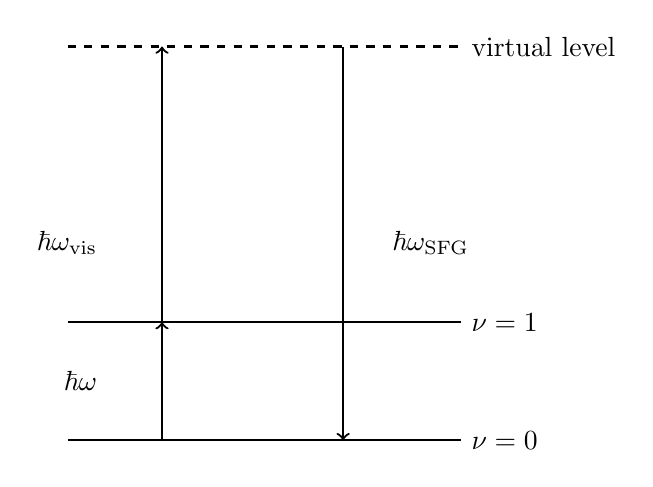
\begin{tikzpicture}[help lines/.style={thin,draw=black!50}]
%%\draw[help lines] (0,0) grid (4,4);
\draw [-, thick] (0,0) -- (5,0) node [anchor = west] {$\nu =0$};
\draw (0.5,0.75) node [anchor = east] {$\hbar\omega$};
\draw [-, thick] (0,1.5) -- (5,1.5) node [anchor = west] {$\nu = 1$};
\draw (0.5,2.5) node [anchor = east] {$\hbar\omega_{\text{vis}}$};
\draw [-, thick,dashed] (0,5) -- (5,5) node [anchor = west] {virtual level};
\draw (4.0,2.5) node [anchor = west] {$\hbar\omega_{\text{SFG}}$};
\draw [->, thick] (1.2,0) -- (1.2,1.5);
\draw [->, thick] (1.2,1.5) -- (1.2,5);
\draw [->, thick] (3.5,5) -- (3.5,0);
\end{tikzpicture}
\caption{The schematic diagram of the VSFG process which involves IR and Raman transitions. The $\nu =0$, $\nu=1$ levels denote the ground and the first excited state of the oscillator\cite{Gang202104}, respectively.
 The dashed line denotes a virtual electronic state in the Raman transition.
}\label{fig:sfg_1a} 
\end{figure}
%
Because experiments usually employed visible and the VSFG frequencies are far from resonant 
conditions, $\chi^{(2),\text{NR}}$ can be considered totally off-resonant and therefore 
insensitive to the laser beams' frequencies involved. Therefore, we can neglect the 
frequency dependence of the non-resonant term.
The molecular information is contained in the resonant signal. The resonant susceptibility $\chi^{(2),\text{R}}(\omega)$ is given by 
\begin{equation}
  \chi_{\eta\xi\kappa}^{(2),\text{R}}(\omega)=\frac{-i}{\hbar}\int_0^\infty dt e^{i\omega t} \text{Tr}{[\rho,\mu_\kappa]\alpha_{\eta\xi}(t)},
\label{eq:chi_R}
\end{equation}
where the index $\eta$, $\xi$ and $\kappa$ are one of $x, y$ and $z$ labels of the laboratory coordinate frame.
In Eq.\thinspace(\ref{eq:chi_R}) $\rho=e^{-\beta H}/Z$ for a system with Hamiltonian $H$ and partition function $Z$ at reciprocal temperature $\beta=1/k_BT$;
$\mu_\kappa$ is the $\kappa$-th component of the system electric dipole and ${\alpha_{\eta\xi}}$ is the $\eta\xi$-th component of the polarizabiltiy tensor\cite{1995SM}.
Besides the vibrational resonance, $\chi^{\text{(2),R}}$, which reflects the vibrational and orientational characteristics of the surface species, 
the VSFG signal also includes the contribution from the non-resonant signal background $\chi^{\text{(2),NR}}$, 
due to static hyperpolarizability of the interface itself\cite{Che2012}.  
For example, there are strong non-resonant second-order nonlinear responses\cite{Pradier11,Vanselow2012,Wieckowski99} of the interface in the case of some metal(-oxide). 
Generally, experiments employ visible light and VSFG frequencies far from resonant conditions, therefore, the non-resonant 
term $\chi^{\text{(2),NR}}$ is approximately off-resonant to the light frequencies involved\cite{Morita02}.
%Neglecting the frequency dependence of the nonresonant term $\chi^{\text{(2),NR}}$ is usually a good approximation. 

\paragraph{Microscopic expression of molecular hyperpolarizability} 
As the electric field is increased, the description of the induced dipole moment 
$\boldsymbol \mu$ should include the normally insignificant nonlinear terms. We can express the induced dipole moment as
\begin{equation}
  {\boldsymbol \mu} = {\boldsymbol \mu}_0 +\alpha {\bf E} + \beta {\bf E E}.
\label{eq:induced_mu}
\end{equation}
%or
%\begin{equation}
%  \mu_i = (\mu_0)_i +\alpha_i  E_i + \beta_{ijk}E_j E_k + \cdots.
%\label{eq:induced_mu}
%\end{equation}
The VSFG spectra are determined by the frequency-dependent hyperpolarizability in molecular level description. 
The frequency-dependent hyperpolarizability can be expressed as a sum of resonant and non-resonant terms:
\begin{equation}
\beta_{\eta\xi\kappa}(\omega_{\text{SFG}},\omega_{\text{vis}},\omega)=\beta_{\eta\xi\kappa}^{\text{R}}+\beta_{\eta\xi\kappa}^{\text{NR}},
\label{eq:beta}
\end{equation}
where $\eta$, $\xi$ and $\kappa$ are space-fixed axes.
The resonant term of the frequency-dependent hyperpolarizability is 
\begin{equation}
  \beta_{\eta\xi\kappa}^{\text{R}}(\omega_{\text{SFG}},\omega_{\text{vis}},\omega)=\sum_{v',v}\frac{\langle v|\alpha_{\eta\xi}|v'\rangle\langle v'|\mu_{\kappa}|v\rangle}{(\omega_{v'}-\omega_v)-\omega-i\gamma_{v'v}}\rho_v,
\label{eq:beta_R}
\end{equation}
where the subscripts $\eta$, $\xi$ and $\kappa$ denote body-fixed axes,
$\omega_{v'}-\omega_v$ is the vibrational energy gap, 
$\rho_v$ is the thermal distribution function of the initial vibrational states $v$,
$\alpha_{\eta\xi}$ is the $\eta\xi$-th component of the molecular dipole polarizability,
$\mu_{\kappa}$ is the $\kappa$-th component of the molecular dipole moment,
and $\gamma_{v'v}$ is the damping rate.
Since  
(see Appendix \ref{calculation_of_chi}) 
\begin{align}
\int_0^\infty dt e^{-it[(\omega_{v'}-\omega_v)-\omega-i\gamma_{v'v}]}=\frac{-i}{(\omega_{v'}-\omega_v)-\omega-i\gamma_{v'v}},
\label{integral_identity1a}
\end{align}
we can rewrite Eq.\thinspace(\ref{eq:beta_R}) as 
\begin{align}
  \beta_{\eta\xi\kappa}^{\text{R}}&=i\int_0^\infty dt \sum_{v'v}e^{-i[(\omega_{v'}-\omega_v)-\omega-i\gamma_{v'v}]t} \langle v|\alpha_{\eta\xi}|v'\rangle\langle v'|\mu_{\kappa}|v\rangle \rho_v \nonumber\\
   &=i\int_0^\infty dt \sum_{v'v}e^{i\omega t} \langle v|e^{iHt}\alpha_{\eta\xi}e^{-iHt}|v'\rangle\langle v'|\mu_{\kappa}|v\rangle \rho_v \nonumber\\
   &=i\int_0^\infty dt e^{i\omega t} \langle\alpha_{\eta\xi}(t)\mu_{\eta\xi}(0)\rangle,
\label{eq:beta_R_b}
\end{align}
where $H$ is the Hamiltonian of the system without external field. 
Eq.\thinspace(\ref{eq:beta_R_b}) indicates that the resonant term $\beta_{\eta\xi\kappa}^{(2),\text{R}}$ is the FT 
of the quantity $\langle\alpha_{\eta\xi}(t)\mu_{\kappa}(0)\rangle$, i.e., the ensemble average of the time correlation function $\alpha_{}(t)\mu_{r}(0)$.
The damping rate $\gamma_{v'v}$ is not explicitly included in Eq.\thinspace(\ref{eq:beta_R_b}), because the dephasing is incorporated in the time development of the off-diagonal matrix elements 
of $\alpha_{\eta\xi}(t)$ and $\mu_{\kappa}(0)$.

The tensor elements $\chi^{(2),R}_{\eta\xi\kappa}$ is microscopically represented as the average sum of first-order hyperpolarizability of the constituent molecules $\beta$ in the space-fixed frame
\begin{align}
  \chi^{(2),R}_{\eta\xi\kappa} = \langle \sum_i^N \sum_{pqr} D_{\eta p}(\Omega_i) D_{\xi q}(\Omega_i) D_{\kappa r}(\Omega_i) \beta_{pqr}\rangle
\label{average_sum}
\end{align}
where $D(\Omega_i)$ is the direction cosine matrix of the $i$-th molecule, projecting $\beta$ onto the space-fixed frame\cite{Morita2000}.

%and evaluate it with the static hyperpolarizability, which can be calculated by an \abinitio Molecular Orbital (MO) package\cite{Morita02}, 
%\begin{equation}
%        \beta_{\eta\xi\kappa}^{\text{NR}}=\sigma\beta_{\eta\xi\kappa}^{\text{static}},
%\label{eq:beta_NR}
%\end{equation}
%where $\sigma$ is the symmetry number among the indices $\eta$, $\xi$ and $\kappa$.
%\paragraph{Derive the value of $\sigma$}
%The frequency-dependent hyperpolarizability, $\beta(\omega_1,\omega_2,\omega_3)$, satisfies the following equation 
%\begin{equation}
%\label{eq:beta_condition}
%        P_p(\omega_1)=\sum_q\alpha_{pq}(\omega_1)E_q(\omega_1)+\sum_{qr}\beta_{pqr}(\omega_1,\omega_2,\omega_3)E_q(\omega_2)E_r(\omega_3)+\cdots
%\end{equation}
%where the suffices $p$, $q$ and $r$ range over $x$, $y$ and $z$, and $P_p(\omega_1)$ is the induced dipole moment at frequency $\omega_1$. The static polarizability and hyperpolarizability are defined as 
%\begin{equation}
%        \alpha_{pq}^{\text{static}}=(\frac{\partial P_p}{\partial E_q})_{E=0},\ \
%        \beta_{pqr}^{\text{static}}=(\frac{\partial^2 P_p}{\partial E_q \partial E_r})_{E=0}
%\label{eq:beta_condition}
%\end{equation}
%and thus the dipole moment in a static external electric field is expressed as 
%\begin{equation}
%        P_p^{\text{static}}=(P_p)_{E=0}+\sum_q\alpha_{pq}^{\text{static}}E_q+\frac{1}{2}\sum_{qr}\beta_{pqr}^{\text{static}}E_qE_r+\cdots,
%\label{eq:static_dipole_moment}
%\end{equation}
%where $(P_p)_{E=0}$ is the permanent dipole moment. From Eq. (\ref{eq:beta_condition}) and Eq. (\ref{eq:static_dipole_moment}), we obtain $\sigma=1/2$ in Eq. (\ref{eq:beta_NR}).

\paragraph{The Fresnel Factors}
Because of screening and dipole-dipole coupling, the local electric fields felt by molecules is different from the macroscopic fields\cite{Vanselow2012}. 
The VSFG signal depends on the magnitude of the local electric fields of the interacting optical beams at the interfaces. 
While the magnitude of the local electric fields is related to both the intensity of the incident beams and the linear refractive indices 
of the different layers (bulk) of the sample\cite{Khatib16}. The Fresnel coefficients define the magnitude of the electric fields at the interface. 
Therefore, to find out the magnitude of the local electric fields, we need to evaluate the Fresnel factors. 
The VSFG intensity $I_{\text{SFG}}$, is proportional to the intensities of the incident visible and infrared beams, $I_{\text{vis}}$, $I$, 
and to the square of the second-order nonlinear susceptibilities,
$\chi_{\eta\xi\kappa}^{(2)}(\omega_{\text{SFG}})$, of the interface:
\begin{equation}
        \chi_{\eta\xi\kappa}^{(2)}(\omega_{\text{SFG}})\propto|\sum_{\eta,\xi,\kappa}L_{\eta\eta}(\omega_{\text{SFG}})\chi_{\eta\xi\kappa}^{(2)}(\omega_{\text{SFG}})L_{\xi\xi}(\omega_{\text{vis}})L_{\kappa\kappa}(\omega)|^2\text{sec}^2(\theta_{\text{SFG}})I_{\text{vis}}I
\label{eq:chi}
\end{equation}
where $\eta$, $\xi$, $\kappa$ are the Descartes coordinates of the reference frame;
$\omega_{\text{SFG}}=\omega_{\text{vis}}+\omega$ is the frequency of VSFG beam; 
$L_{\eta\eta}$, $L_{\xi\xi}$ and $L_{\kappa\kappa}$ are the Fresnel coefficients; 
$\theta_{\text{SFG}}$ is the reflected angle of VSFG beam with respect to the normal 
direction in the medium.

\subsection{VSFG spectra from velocity auto-correlation functions}
%To construct SFG spectrum of O-H stretching at the water/vapor interface and to ascertain the molecular origin of SFG spectrum, 
%quantum corrected time correlation function \cite{Morita02,Morita04} and instantaneous normal mode (INM) methods are used 
%by Perry and coworkers.\cite{Perry03} 
%For  water/vapor interface, the INM SFG spectrum is in agreement with the time correlatin function SFG spectrum. 
%This implies that motional narrowing effects play little role  in the interfacial line shape. The Shen group suggests that 
%the motional narrowing effects may be significant in the SPS geometry, where the "free O-H" stretching peak is greatly diminished.\cite{WeiX02}
%========================
%\section{solutions}
%Here we discuss the calculation of nonlinear susceptibility of water molecules at liquid/vapor interfaces.
%The SFG spectrum is proportional to the square of the nonlinear susceptibility of water molecules at the water/vapor interface. \cite{QD94}  
%Details:
This paragraph gives the derivation an expression for the calculation of the sum frequency generation spectra of water interfaces that is
based on the projection of the atomic velocities on the local normal modes, such an approach permits one to obtain the VSFG signals from suitable
VACFs, reducing the computational cost to that of the accumulation of a molecular dynamics trajectory, and therefore cutting 
the overhead costs associated with the explicit calculation of the dipole and polarizability tensor. Moreover, the method permits to interpret 
the peaks in the spectrum in terms of local modes.
The components of the resonant term $\chi^{\text{(2),R}}_{\eta\xi\kappa}$ of the second order susceptibility can be calculated 
according to the classical formula\cite{Morita02,Morita2008,Nihonyanagi2011}
\begin{align}
  \chi^{\text{(2),R}}_{\eta\xi\kappa}&=\frac{-i}{k_{\text{B}}T \omega} \int_0^\infty dt e^{i\omega t}\left\langle \dot{A}_{\eta\xi}(t) \dot{M}_{\kappa}(0)\right\rangle 
 \label{eq:chi}
\end{align}
%\begin{align}
% \chi^{(2)}_{XXZ,R}&=\frac{i}{k_BT \omega} \sum\limits_j \int_0^\infty dt e^{i\omega t} \left \langle \frac{\partial A_{XX}}{\partial r_j} \frac{\partial M_Z}{\partial r_j}  \dot{r}_j(0) \dot{r}_j(t) \right\rangle
% \label{eq:chi2}
% \end{align}
where $k_{\text{B}}$ is the Boltzmann constant, $\omega$ is the frequency of the IR beam, ${\bf M}$ (${A}$) is the dipole 
moment (dipole polarizability) of the system, and $\left\langle\dots\right\rangle$ denotes the average over all starting time points. 
%The derivation of Eq.\thinspace(\ref{eq:chi}) is given in Appendix \ref{calculation_of_chi}.
 
 The total dipole moment and dipole polarizability derivatives for the system can be expressed in terms of the water and bond contributions:
\begin{align}
 \dot{A}&=\sum_{i=1}^N \sum_{\epsilon}\dot{\alpha}^{i,\text{l},\epsilon} \\ 
 \dot{{\bf M}}&=\sum_{i=1}^N \sum_{\epsilon}\dot{\mu}^{i,\text{l},\epsilon} 
 \label{eq:A-M}
\end{align}
where ${\mu}^{i,\text{l},\epsilon}$ (${\alpha}^{i,\text{l},\epsilon}$) is the dipole moment (polarizability)
of the bond $\epsilon$ of the $i$-th water molecule, the superscript (l) denote these quantities are measured in the 
lab frame, and $N$ is the total number of water molecules.
Therefore, the correlation function in Eq.\thinspace(\ref{eq:chi}) can be written as 
\begin{align}
  \langle\dot{A}_{\eta\xi}(t)\dot{M}_{\kappa}(0)\rangle 
    &=\sum_{i=1}^N \sum_{\epsilon}\left\langle\dot{\alpha}_{\eta\xi,i,\epsilon}^{\text{l}}(t)\dot{\mu}_{\kappa,i,\epsilon}^{\text{l}}(0)\right\rangle \nonumber \\ 
    &+\sum_{i=1}^N \sum_{\epsilon}\left\langle\dot{\alpha}_{\eta\xi,i,\epsilon}^{\text{l}}(t)\dot{\mu}_{\kappa,i,-\epsilon}^{\text{l}}(0)\right\rangle \nonumber \\
    &+\sum_{i,j=1;i\neq j}^N \sum_{\epsilon,\epsilon'}\left\langle\dot{\alpha}_{\eta\xi,i,\epsilon}^{\text{l}}(t)\dot{\mu}_{\kappa,i,\epsilon'}^{\text{l}}(0)\right\rangle.
 \label{eq:correl_AM}
 \end{align}
In Eq.\thinspace(\ref{eq:correl_AM}), the first term of the right-hand side is the bond auto-correlation, the second term accounts 
for the correlation between the two bonds in the same water molecule, and the third them for the correlation between 
bonds in two different water molecules.
 
We assume that the bond elongation are small compared to the total bond length and stretching frequencies of the bond are 
much larger than frequencies of bond reorientation, for example, the libration.
Therefore, we can approximately write ${\dot\mu}(0)$ by 
\begin{align}
    \dot\mu_{\kappa}(0)&=\sum_i^{x,y,z}{{D}}_{\kappa i}(0)\dot{\mu}_i(0) \nonumber \\
                       &=\sum_i^{x,y,z}{{D}}_{\kappa i}(0)\biggl(\sum_j^{x,y,z}\frac{d\mu_i}{d r_j}\frac{d{r}_j}{dt}|_{t=0}\biggr) \nonumber \\
                       &=\sum_{i}^{x,y,z}{{D}}_{\kappa i}(0)\frac{d\mu_i}{dr_z}v_z(0),
    \label{eq:dot_mu}
 \end{align}
where ${D}_{\kappa i}$ is the direction cosine between the laboratory-fixed $\kappa$ axis and the molecular-fixed $i$ axis,
and $v_z=\frac{d{r}_z}{dt}|_{t=0}$ is the projection of the velocity on the bond axis.

Similarly, for the dipole polarizability, we have
\begin{align}
  \dot\alpha_{\eta\xi}(t)&=\sum_{i,j}^{x,y,z} \biggl({D}_{\eta i}(t)\frac{\partial\alpha_{ij}}{\partial r_z}{D}_{\xi j}(t)\biggr)v_z(t). 
  \label{eq:dot_alpha}
 \end{align}
The Eq.\thinspace(\ref{eq:dot_mu}) and Eq.\thinspace(\ref{eq:dot_alpha}) simplify the calculation of the  
$\left\langle \dot{A}_{\eta\xi}(t) \dot{M}_{\kappa}(0)\right\rangle$ in Eq.\thinspace(\ref{eq:chi}), because $v_z(t)$
and ${D}(t)$ can be readily determined from the DFTMD
trajectory, and $\frac{d\mu_i}{dr_z}$ and $\frac{d\alpha_{ij}}{dr_z}$ can be parameterized\cite{Corcelli05,Khatib16}.
%
\begin{figure}
\centering
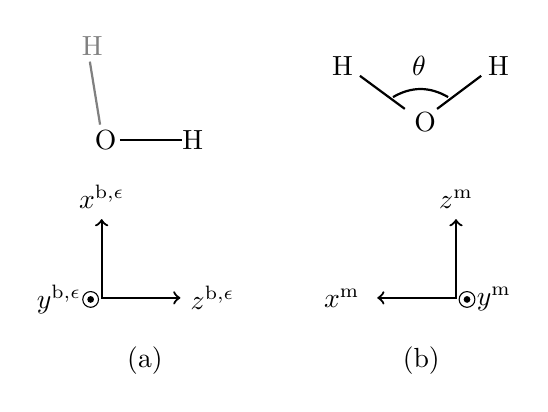
\begin{tikzpicture}[help lines/.style={thin,draw=black!50}]
%\draw[help lines] (0,0) grid (4,4);
%a
\draw [<->,thick] (0,1) node (xaxis) [above] {$x^{\text{b},\epsilon}$}
  |- (1,0) node (zaxis) [right] {$z^{\text{b},\epsilon}$};
  \filldraw[black] (-0.14,-0.02) circle (1pt) node [anchor=east] {$y^{\text{b},\epsilon}$};
\draw(-0.14,-0.02) circle (0.1);
\draw (0.2, -0.8) node [anchor=west] {(a)};
% H2O
\draw[gray,thick] (-0.02, 2.2) coordinate (a_1) -- (-0.15, 3) coordinate (a_2);
\draw[thick] (0.23, 2) coordinate (b_1) -- (1.02, 2) coordinate (b_2);
\draw (0.31, 2) node [anchor=east] {O};
\draw (0.9, 2) node [anchor=west] {H};
\draw[gray] (-0.12, 2.95) node [anchor=south] {H};
%\draw (0.56, 2.61) node {\chemfig{[:-84]H-O-[:0]H}};
%b
\draw [<->,thick] (3.5,0)--(4.5,0) node (xaxis){} 
  |- (4.5,0)--(4.5,1) node (zaxis) [above] {$z^{\text{m}}$};
  \filldraw[black] (4.64, -0.02) circle (1pt) node [anchor=west] {$y^{\text{m}}$};
\draw (2.7, 0) node [anchor=west] {$x^{\text{m}}$};
\draw(4.64,-0.02) circle (0.1);
\draw (3.7, -0.8) node [anchor=west] {(b)};
% H2O
\draw[thick] (3.85, 2.4) coordinate (a_1) -- (3.28, 2.82) coordinate (a_2);
\draw[thick] (4.26, 2.4) coordinate (b_1) -- (4.82, 2.82) coordinate (b_2);
\draw[thick] (3.7,2.55) to [out=30,in=150] (4.4,2.55);
\draw (4.03, 2.7) node [anchor=south] {$\theta$};
\draw (4.37, 2.23) node [anchor=east] {O};
\draw (5.04, 2.7) node [anchor=south] {H};
\draw (3.06, 2.7) node [anchor=south] {H};
%\draw (4.06, 2.61) node {\chemfig{[:-37]H-O-[:37]H}};
\end{tikzpicture}
  \caption{\label{fig:frameworks} The representation of the bond (a) and the molecular (b) frameworks. (from Ref. \cite{Khatib2017})}
\end{figure}

%
We used three different frameworks: the lab framework ($x^{\text{l}},y^{\text{l}},z^{\text{l}}$), the molecular framework 
($x^{\text{m}},y^{\text{m}},z^{\text{m}}$) and the bond framework ($x^{\text{b}},y^{\text{b}},z^{\text{b}}$) (see Fig.\thinspace\ref{fig:frameworks}).
In the lab framework, the $z^{\text{l}}$-axis is perpendicular to the interface. 
The molecular frame will be used to decompose the signal into normal modes of water monomers. 
For the $j$-th molecule, the $z^{\text m}$ axis is along the bisector of the H-O-H angle, the $x^{\text m}$ axis is in the molecular plane, 
and the $y^{\text m}$ axis is out of the molecular plane\cite{Khatib2017}. 

In the bond framework, $z^{\text{b},\epsilon}$ axis is along the bond $\epsilon$ of a molecule, $z^{\text{b},\epsilon}$
is in the molecular plane and $y^{\text{b},\epsilon}$ is out of the molecular plane.
\begin{align}
  \dot{\alpha}^{\text{l},\epsilon} &= {{D}}^{\text{m}}{{D}}^{\text{b},\epsilon}(\frac{\partial{\alpha}^{\text{b}}}{\partial r}\dot
    r^{\epsilon})({D}^{\text{b},\epsilon})^{\text{T}}({D}^{\text{m}})^{\text{T}}, \\ 
    \dot\mu^{\text{l},\epsilon} &= {{D}}^{\text{m}}{{D}}^{\text{b},\epsilon}(\frac{\partial \mu^{\text{b}}}{\partial r}\dot r^{\epsilon}).
    \label{eq:dot_mu-alpha}
 \end{align}
The direction cosine matrix ${{D}}^{\text{b},\epsilon=1}$ and ${{D}}^{\text{b},\epsilon=-1}$ can be expressed as 
\begin{equation}
    {{D}}^{\text{b},1}=\left(
                \begin{matrix}
                    \text{cos}\frac{\theta}{2} &  0  & -\text{sin}\frac{\theta}{2}\\
                    0 & 1 & 0\\
                    \text{sin}\frac{\theta}{2} & 0 & \text{cos}\frac{\theta}{2}
\end{matrix}
\right),\quad
    {{D}}^{\text{b},-1}=\left(
         \begin{matrix}
             -\text{cos}\frac{\theta}{2} & 0 & \text{sin}\frac{\theta}{2}\\
             0 & 1 & 0\\
             \text{sin}\frac{\theta}{2} & 0  & \text{cos}\frac{\theta}{2}
\end{matrix}
\right),
\label{eq:D_b}
\end{equation}
where $\theta$ is the H-O-H angle in a water molecule.
%The approximate value of the angle is 105.5$^\circ$.
We use ${{D}}^{\text{m}}$ to transform the coordinates in a molecular framework to coordinates in the lab framework. 
Because the orientation of water molecules is changing during the simulation, 
%the angle $\theta'_i$ between the water dipole moment and the $z$-axis is time dependent, therefore, 
${{D}}^{\text{m}}$ is time dependent. 
%It can be expressed as 
%\begin{equation}
%    {\bf{D}}^{\text{m}}=
%    \left(
%        \begin{matrix}
%            \text{cos}{\gamma} & \text{sin}{\gamma} & 0\\
%            -\text{sin}{\gamma} & \text{cos}{\gamma} & 0\\
%            0 & 0 & 1
%        \end{matrix}
%     \right)
%     \left(
%         \begin{matrix}
%             \text{cos}{\theta'} & 0 & -\text{sin}{\theta'}\\
%             0 & 1 & 0\\
%             \text{sin}{\theta'} & 0  & \text{cos}{\theta'}
%         \end{matrix}
%     \right) 
%     =
%     \left(
%         \begin{matrix}
%             \text{cos}{\gamma}\text{cos}{\theta'} & \text{sin}{\gamma} & -\text{cos}{\gamma}\text{sin}{\theta'}\\
%             -\text{sin}{\gamma}\text{cos}{\theta'} & \text{cos}{\gamma} & \text{sin}{\gamma}\text{sin}{\theta'}\\
%             \text{sin}{\theta'} & 0  & \text{cos}{\theta'}
%         \end{matrix}
%     \right),
%\label{eq:D_m}
%\end{equation}
%where $\gamma$ is the angle between the incident plane (x-z plane) and the molecular plane of a water molecule,
%and $\theta'$ is the angle of the dipole moment of the water molecule from the normal direction of the interface, 
%and both $\gamma$ and $\theta'$ are time dependent.

Based on DFTMD simulations, we can implement the parameterization of $\frac{\partial \mu_{k}}{\partial r_z}$ and $\frac{\partial\alpha_{ij}}{\partial r_z}$
and calculate the correlation function $\langle\dot{A}_{\eta\xi}(t)\dot{M}_{\kappa}(0)\rangle$ through the velocity auto-correlation function. 
This approximation for estimating the susceptibility retains the details of the interface, including the full electronic structure. 
And it reduces the computational cost for a total calculation with the instantaneous evaluation of the molecular dipoles and polarizabilities\cite{sulpizi2013}. 
The parametrization of $\frac{\partial \mu_{k}}{\partial r_z}$ and $\frac{\partial\alpha_{ij}}{\partial r_z}$ is based 
on the calculation of the MLWF\cite{Marzari97} 
 and can be done through the approach developed by Salanne \etal\cite{Salanne08} and Khatib \etal\cite{Khatib2017}.
The implementation of this parametrization is given in Appendix \ref{calculate_derivatives}.
%\paragraph{Calculation of $\chi^{(2)}$ (Method 2)}
%We now consider the velocities projection on the water normal modes, identified by the collective variables ${\bf{R}}_j$ in the molecular framework. 
%The single water molecule has nine normal modes. Six of them have the angular frequencies $\omega$ equal zero and three normal modes remains. 
%The three normal modes are the symmetric stretching (SS), the antisymmetric stretching (AS) and the bending (B).
%The dipole moment and the molecular polarizability of the $i$th water molecule can be rewritten as
%\begin{align}
%    \dot{\bf \alpha}_{i}^{\text{l}}(t)&={\bf{D}}_{\text{m},i}(\sum_{j=Q,SS,AS}\frac{\partial{\bf\alpha}_{i}^{\text{m}}}{\partial R_j}){\bf{D}}^{\text{T}}_{\text{m},i}, \\ 
%    \dot{\bf \mu}_{i}^{\text{l}}&={\bf{D}}_{\text{m},i}(\sum_{j=Q,SS,AS}\frac{\partial{\bf\mu}_i^{\text{m}}}{\partial R_j}\dot{R}_j).  
%    \label{eq:dot_mu_alpha}
%\end{align}
%where $i$ denote the $i$-th water molecule.
%To parametrize the derivatives $\frac{\partial \alpha_i^{\text{m}}}{\partial R_j}$ and $\frac{\partial {\bf{\mu}}_i^{\text{m}}}{\partial R_j}$,
%the Maximally Localized Wannier Functions (MLWF) were emplyed.\cite{Salanne08,Khatib2017}


\section{Definitions of HB population and correlation functions}\label{section:def_HBP}
Luzar and Chandler\cite{AL96} have pioneered the analysis of the HB dynamics of pure water, and
subsequently such analysis has been extended to more complex systems, e.g., electrolytes\cite{Chandra2000}, proteins\cite{Tarek02,Matthias13}, 
biomolecules\cite{Kolano06} and micellar surfaces\cite{SP05}.
There are geometric\cite{Kumar2007} and energetic\cite{Sciortino1989} criteria to define a HB.
Here we use the geometric one:
Two water molecules are H-bonded if their inter-oxygen distance between a specific tagged pair of water molecules 
is less than cutoff radius $r^{\text{c}}_{\text{OO}}$ and
the H-O$\cdots$O angle is less than cutoff angle $\phi^{\text{c}}$\cite{AKS86,JT90,SB02}. 
The value $r^{\text{c}}_{\text{OO}}$ corresponds to the first-minimum position of the O--O Radial Distribution Function (RDF) of water\cite{Sciortino1989}.   
The choice for $\phi^{\text{c}}$ for water-water molecules is obtained by studying the average number of H-bonds,
as a function of $\phi^{\text{c}}$\cite{Luzar1993}. We call this definition of HB the Acceptor-Donor-Hydrogen (ADH) criterion. 
To compare the impact of different HB definitions on HB dynamics, we also use another definition of HB in our analysis. 
When the distance between the oxygen atoms of two water molecules is less than $r^{\text{c}}_{\text{OO}}$, 
and the O-H$\cdots$O included angle is greater than cutoff angle $\theta^{\text{c}}$, then we say that there is a HB between the two molecules. 
We denote this definition as the Acceptor-Hydrogen-Donor (AHD) criterion.
In this thesis, we use $r^{\text{c}}_{\text{OO}}=3.5$ \AA both for the ADH and AHD criteria, $\phi^{\text{c}}=30^{\circ}$ for the ADH criterion, 
and $\theta^{\text{c}}=120^{\circ}$ for the AHD criterion.

% introduce h(t)
The configuration criterion above allows us to define a variable $h[r(t)] = h(t)$, the HB population. 
Here a configuration $r(t)$ denotes the positions of all the atoms in the system at time $t$\cite{AL96}.  
The $h(t)$ has a value 1 when the particular tagged pair of molecules are bonded, and 0 otherwise. 
%=================
% added 2020-5-27: to show that h(t) is actually the fluctuation of itself (\delta h).
The fluctuation or deviation in the dynamical variable $h(t)$ from its time-independent equilibrium average $\langle h\rangle$ , 
is defined by\cite{DC87} 
$$
\delta h = h(t) - \langle h\rangle.
$$
Since the probability that a specific pair of molecules is bonded in a large system is extremely small, i.e., 
the time average of $h$ is zero, or  
$\langle h \rangle = 0$,
then
$$
\delta h(t) = h(t).
$$
Therefore, $h(t)$ describe the fluctuation $\delta h(t)$  of the HB population.  
%=================

While the equilibrium average of $\delta h(t)$ is zero, we can obtain useful information by considering the equilibrium 
correlations between fluctuations at different times. The correlation between $\delta h(t)$ and $\delta h(0)$ can be written as 
$$
\langle \delta h(0) \delta h(t)\rangle = \langle h(0)h(t)\rangle-\langle h \rangle^2 = \langle h(0)h(t)\rangle,
$$
where the averaging $\langle\cdots\rangle$ is to be performed over the ensemble of initial conditions.% $(r^N, p^N)$.


In this paragraph, we use the following three correlation functions to describe the HB dynamics of the water/vapor interface:
the HB population auto-correlation function \CHB, the continuum HB population correlation function (also called survival probability) 
\SHB and the reactive flux $k(t)$\cite{Rapaport1983}.

\FloatBarrier
\paragraph{Hydrogen bond population auto-correlation function}
The auto-correlation function \CHB of the HB population is used to describe the structural relaxation of H-bonds. It is defined by 
\begin{eqnarray}
c(t)=\langle h(0)h(t) \rangle/\langle h\rangle
\label{eq:C_HB}.
\end{eqnarray}
With the aid of the ergodic principle, the ensemble average $\langle \cdots\rangle$ is implemented by time average.
The $\langle h\rangle$ is the probability that a pair of randomly chosen water molecules in the system is
H-bonded at any time $t$. 
As examples, the dynamics of the interoxygen distance $r_{\text{OO}}(t)$, 
the cosine of the H$-$O$\cdots$O angle (cos$\phi(t)$)  
and the HB population operator $h(t)$ for a HB in a DFTMD simulated water cluster (H$_2$O)$_n$ (n=5) 
at 300 K is displayed in Fig.\thinspace\ref{fig:Ex30ps_hb}, respectively.
%-------------------
\begin{figure}[hbtp]
\centering
\includegraphics [width=0.42\textwidth] {./diagrams/Ex30ps_hb}
\setlength{\abovecaptionskip}{0pt}
\caption{\label{fig:Ex30ps_hb}Dynamics of $r_{\text{OO}}(t)$ (top panel), cos$\phi(t)$ (middle panel), 
  and $h(t)$ (bottom panel) for a typical HB in a water cluster. The dashed lines show the interoxygen distance 
  boundary $r^{\text{c}}_{\text{OO}}$=3.5 \AA (top panel) and criterion of cosine of H$-$O$\cdots$O angle cos$\phi^{\text{c}}$ 
  with $\phi^{\text{c}}$=30$^{\circ}$ (middle panel), respectively.}
\end{figure} 

In a large system that consists of many water molecules, the probability that a specific pair of water molecules are H-bonded is extremely small. 
Therefore, the \CHB relaxes to zero when $t$ is large. 
The \CHB measures correlation in $h(t)$ independent of any possible bond breaking events. 
This function is one of the intermittent HB correlation functions, introduced by Stillinger, Rapaport 
and others\cite{Stillinger1975,Rapaport1983,Geiger1984,Zichi1986,Sciortino1989,Sciortino1990,Starr2000,vanderSpoel2006,Busch2021},
and can be studied by a continuous function, the probability density.
From \CHB, the HB relaxation time $\tau_{\text{R}}$ can be computed by
\begin{eqnarray}
  \tau_{\text{R}} &=& \frac{\int t c(t)\text{d}t}{\int c(t)\text{d}t}.
\label{eq:tau_relaxation}
\end{eqnarray}

The \CHB for the simulated bulk water is shown in Fig.\thinspace\ref{fig:pure_bk_c_from_2_methods} a 
(For computational details, see Appendix\thinspace\ref{DETAILS_NEAT_WATER}).
We can obtain the relaxation time from Eq.\thinspace\ref{eq:tau_relaxation}: $\tau_R = 14.01$ ps for the ADH definition, 
and $\tau_R = 14.16$ ps for the AHD definition. 
\begin{figure}[H]
\centering
\includegraphics [width=0.6\textwidth] {./diagrams/pure_bk_c_from_2_methods}
\setlength{\abovecaptionskip}{0pt}
\caption{\label{fig:pure_bk_c_from_2_methods}
The \CHB for bulk water, as computed from the ADH (solid line) and AHD (dashed line) criterion of H-bonds. 
(a) the interchange processes are included; (b) The interchange processes are neglected.}
%\caption{\label{fig:128w_c_itp_bk_ns40}Time dependence of \CHB for bulk water at 300 K with density $\rho =1.00$ g/cm$^3$.} 
%The length of the trajectory is 35 ps of physical time. Ref:\cite{Khaliullin2013}}
\end{figure} 

The method of HB population-based HB dynamics used in this section has been frequently used in previous literature\cite{Luzar1994,AL96,Chandra2000}. 
The basis is the population operator $h(t)$ of the HB formed between two water molecules. 
The function \CHB is interpreted as the probability that the HB is intact at time $t$, 
if the pair of water molecules are H-bonded at time zero. 

%Besides $h(t)$, here we also discuss another possible definition of the HB population operator ${h}'(t)$.
When a pair of water molecules $a$ and $b$ are H-bonded, 
there are 4 different forms of possible H-bonds . 
In other words, there are exchange processes, i.e., interchange tunneling and bifurcation tunneling, during the dynamics.
After an exchange process, a pair of bonded molecules still form H-bonds.
%we say that an old HB is broken and a new HB is formed.
In the above definition, we have not included this interexchange process, i.e., the H-bonds before and after the interexchange process are regarded as the same HB.
If we consider this interexchange process in the definition of HB population, the corresponding function $c(t)$ will be slightly differnt, 
see Fig.\thinspace\ref{fig:pure_bk_c_from_2_methods} b.   
In the next paragraphs, for the sake of simplicity, 
we will ignore this interchange process and simply regard the H-bonds before and after the exchange process as the same HB.
%Fig.\thinspace\ref{fig:pure_bk_c_from_2_methods} a shows the correlation function \CHB for bulk water over time. 
Comparing Fig.\thinspace\ref{fig:pure_bk_c_from_2_methods} a and b,  
we find that the relaxation in the latter is faster than that in the former,
because the bifurcation tunneling (hydrogen exchange) is considered.
%In the following, we will use the original HB population based on O--H bond, instead of water--water molecule pairs, unless otherwise specified.

%%
%\begin{figure} [htbp]
%\centering
%	\includegraphics [width=0.36\textwidth] {./diagrams/bk_water_c_two_population_operators_with_ADH}
%\setlength{\abovecaptionskip}{0pt}
%	\caption{\label{fig:bk_water_c_two_population_operators_with_ADH} The auto-correlation functions of $h(t)$ and ${h}'(t)$ for water molecules in bulk water (ADH criterion). 
%        The HB population is based on two different definitions: $h(t)$ is based on water molecule pair (solid line),\cite{Khaliullin2013} 
%and ${h}'(t)$ is based on O--H pairs (dashed line).}
%\end{figure} 
Besides, in Fig.s\thinspace\ref{fig:pure_bk_c_from_2_methods} a and \ref{fig:pure_bk_c_from_2_methods} b, 
we plotted \CHB for bulk water, using the ADH and AHD criteria of HB. We find that the relaxation tie of H-bonds is not affected by the HB criteria. 
%

Because the thermal motion can cause distortions of H-bonds from the perfectly tetrahedral configuration,
water molecules show a librational motion on a time scale of $\sim$ 0.1 ps superimposed to rotational and diffusional motions ($> 1$ ps), 
which causes a time variation of interaction parameters.
A new HB population $h^{(d)}(t)$ was also defined to obviate the distortion of real HB dynamics\cite{Sciortino1989,Chandra2000}.
The $h^{(d)}(t)$ is 1 when the interoxygen distance of a particular tagged pair of water molecules is less than $r^{\text{c}}_{\text{OO}}=3.5$ \AA at time $t$ and 0 otherwise. 
The difference between the operators $h^{(d)}(t)$ and $h(t)$ is that there is no restriction on the angle. Therefore, those molecular pairs that meet the condition of $h^{(d)}(t)=1$ may not meet the condition of $h(t)=1$.
That is, the H-bonds between the tagged molecular pairs that satisfy the condition $h^{(d)}(t)=1$ may have been broken, but they may more easily form H-bonds again.
The function 
\begin{eqnarray}
  c^{(d)}(t)=\langle h(0)h^{(d)}(t) \rangle/\langle h\rangle
\label{eq:C_HB_d}
\end{eqnarray}
is the probability that the specific two water molecules are located in reformable region ($r_{\text{OO}} < r^{\text{c}}_{\text{OO}}$) at time $t$,
if they were H-bonded at time zero. 
The time correlation function 
%
\begin{eqnarray}
n(t)=\langle h(0)[1-h(t)]h^{(d)}(t) \rangle/\langle h\rangle 
\label{eq:n_HB}
\end{eqnarray}
represents the probability at time $t$ 
that a tagged pair of initially H-bonded water molecules are not bonded but remain separated by less than $r_{\text{OO}}^{\text{c}}$,
$1-h(t)$ describes the breaking of a HB at time $t$ after its formation at time $t=0$.
The probability at time $t$ that a pair of water molecules bonded at the initial moment does not be bonded 
but the distance between their oxygen atoms is still less than $r_\text{OO}^c$ is calculated according to 
\begin{eqnarray}
n(t) = \int_0^t dt'k_\text{in}(t'),
\label{eq:n_from_k_in}
\end{eqnarray}
where $k_\text{in}(t) = -\langle \dot h(0)[1-h(t)]h^d(t) \rangle/\langle h\rangle$ is the restricted rate function. 
%===============================
\FloatBarrier
\paragraph{Continuum HB population correlation function \SHB}
%===============================
Another scheme to describe the HB dynamics is the continuum HB population correlation function \SHB, or survival probability\cite{Chandra2000} for a newly generated HB.
It is defined as
\begin{eqnarray}
s(t)=\langle h(0)H(t) \rangle/\langle h\rangle 
\label{eq:S_HB},
\end{eqnarray}
where $H(t)=1$ if the tagged pair of molecules, remains \emph{continuously} H-bonded till time $t$ 
and 0 otherwise.  It describes the probability that an initially H-bonded molecular pair 
remains bonded at all times up to $t$\cite{Chowdhuri2006}.
The \SHB for the simulated bulk water according to the formula \ref{eq:S_HB} is shown in Fig.\thinspace\ref{fig:128w_s_itp_bk_ns40}.
%
\begin{figure}[hbtp]
\centering
\includegraphics [width=0.36\textwidth] {./diagrams/128w_s_bk_ns40}
\setlength{\abovecaptionskip}{0pt}
\caption{\label{fig:128w_s_itp_bk_ns40} Time dependence of \SHB for bulk water.} 
%The length of the trajectory is 35 ps of physical time.
\end{figure} 

The average continuum HB lifetime $\langle \tau_{\mathrm{a}} \rangle$ is calculated by the integration of \SHB over $t$ (For detailed derivation, see Appendix \ref{diff_distr}.) :  
\begin{eqnarray}
  \langle\tau_{\mathrm{a}}\rangle = \int_0^\infty s(t) dt.
\label{eq:calculate_hb_lifetime_from_s}
\end{eqnarray}
%
The time derivative of \SHB
\begin{eqnarray}
P_a(t) = -\frac{\text{d}s(t)}{\text{d}t}
\label{eq:P_1}
\end{eqnarray}
represents the first passage time probability density of H bonds. $P_a(t)$ is also called probability distribution of HB lifetimes\cite{Sciortino1990prl,Krausche1992,FWS99,Voloshin2009}, or histogram of HB lifetimes\cite{Geiger1984,Stanley2000}.
It denotes the probability of the first HB breaking in time $t$ after it has been detected at $t=0$, i.e.,
\begin{eqnarray}
s(t)= \int_t^\infty P_a(t')dt'.
\label{eq:P_2}
\end{eqnarray}

\FloatBarrier
\paragraph{Reactive Flux $k(t)$} 
The rate of relaxation to equilibrium is characterized by the reactive flux correlation function, 
\begin{eqnarray}
k(t) = -\frac{\text{d}c(t)}{\text{d}t},
\label{eq:k}
\end{eqnarray}
i.e., $k(t)=\langle j(0)[1-h(t)]\rangle/\langle h\rangle$\cite{AL96,AL00},
where 
$j(0)=-\text{d}h/\text{d}t|_{t=0}$ 
is the integrated flux departing the HB configuration space at time $t=0$ (For detailed derivation, see Appendix \ref{calc_rf}.).
The $-k(t)$ is the average rate of change of HB population for the trajectories in which the HB is broken at a time $t$ later\cite{AL96}, 
independent of possible breaking and reforming events in the interval from 0 to $t$.
Therefore, $k(t)$ measures the effective decay rate of an initial set of H-bonds\cite{DC87,Starr2000}.


Assuming that each HB acts independently of other H-bonds\cite{AL96,AL00}, 
thanks to detailed balance condition, we obtain 
\begin{eqnarray}
  \tau_{\text{HB}} &=& \frac{1- \langle h\rangle}{k},
\label{eq:rate}
\end{eqnarray}
where $k$ is the rate constant of breaking a HB (forward rate constant)\cite{Chandler1986,Chandler1978}. 
For an aqueous interface, the probability that a given tagged molecule pair forms a HB is very low, that is, $\langle h\rangle \ll 1$. 
Therefore, $k$ is related to the average HB lifetime by $\tau_{\text{HB}}=1/k$.
Using $k'$ to represent the rate constant from the HB \emph{on} state to the HB \emph{off} state for a tagged pair of molecules (backward rate constant),
the reaction time constant $\tau_\text{re}$ is 
\begin{eqnarray}
  \tau_\text{re} &=& \frac{1}{k+k'}.
\label{eq:reaction_rate_tau}
\end{eqnarray}

 
\chapter{Experimental SFG spectra of salty interfaces}\label{CHAPTER_SFG_Exp}
In this chapter, we will give the experimental results obtained on salty solutions containing alkali cations and nitrate (iodide) anions. \cite{PS03,AJ12,HuaWei2014} 

%We will choose the interface of lithium nitrate solution as our research object, which is a typical example of the interface of alkali metal nitrate solution.
From the experimental data of surface tension dependence on solute concentration $\text{d}\gamma/\text{d}m_2$ 
at low electrolyte concentrations ($\leq$1.5 M ), \cite{Weissenborn95,Hey81,Jarvis68,Jarvis72} 
%and the assumption that \Na is the most excluded cation
the relation of the surface/bulk molar concentration ratio $K_{\text{p}}$ \cite{Pegram2006} among \li, \Na and \K is: 
\begin{equation}
0=K_{\text{p,Na}^+}< K_{\text{p,K}^+}< K_{\text{p,Li}^+}.
\label{eq:bscr}
\end{equation}
i.e., \Na is the most surface-excluded in the water solution RNO$_3$, \K is less excluded, 
and \Li is the least excluded cation. (See \ref{surface_tension_increment} and \ref{gibbs_surface_excess} for details.)
In modeling the interfaces of aqueous sulitons of alkali metal nitrates, we decided to start with LiNO$_3$, because the \Li ion is the least excluded of the vapor-liquid interface 
among the alkali metal ions. 
%
%The aim of our work here is to provide a molecular picture 
%for the water/vapor interface of the \ch{LiNO3}-containing solution 
%to interpret the experimental spectra. In particular a question raises if simple models 
%for the solvated ion clusters can already provide information
%on the ions-water complexes formed at the interface. 
%It is known that nitrate (\nitrate) is a naturally occurring ion which is part of the nitrogen cycle, 
%and it can reach both surface water and groundwater as a consequence of agricultural activity. 
%Nitrate also has effects on human health,  because of the toxicity caused by its reduction to nitrite (NO$_2^-$). \cite{WHO11}
%The biological effect of nitrite in humans is its involvement in the oxidation of
%normal Hb to metHb, which is unable to transport oxygen to the tissues.
%For example, infants who drink water with high levels of nitrate (more than 10 mg/L) may suffer 
%a serious health condition due to blue baby syndrome.\cite{Knobeloch00}
%

%The goal of this chapter is to find the origin of the main characteristics of the VSFG spectra of the \LiN solution,
%and provide a molecular picture to interpret the recorded spectra.
%In order to achieve this goal, we simulate water/vapor interface including \Li and \nitrate, 
%as shown in Fig.\thinspace\ref{fig:interface_chandler},
%and extract the vibrational spectroscopic properties of the water/vapor interface of LiNO$_3$ solution.
%=========
%
%\begin{figure}[htbp]
%\centering
%\includegraphics [width=0.5 \textwidth] {./diagrams/interface_chandler}
%\setlength{\abovecaptionskip}{0pt}
%\caption{\label{fig:interface_chandler} The water/vapor interfaces of \LiN solution and pure water. 
%The right panel shows that the \Li and the \nitrate ions are separated by a water molecule at the salty interface.}
%\end{figure}
%The water molecules below 4 \AA  of the instantaneous interfaces are shown opaquely. 

%
Hua \etal \cite{HuaWei2014} have recently measured the VSFG spectra of water/vapor interface of \LiN salt solutions in the OH stretching region
(3000--3800 \centimeter) using Heterodyne Detected VSFG spectroscopy. \cite{HuaWei2011,HuaWei2011b,ChenXiangKe2010} 
The experimental result of the VSFG intensity of the alkali nitrate interfaces is given by in Fig.\space\ref{fig:Allen12}. 
At a difference with the spectra for the water interface, in the spectra of 
\LiN solutions, a depletion of the 3200 \cm peak is observed, with an 
enhancement of the 3400 \cm peak.
A similar behaviour had been observed for the interface of NaNO$_3$ and 
Mg(NO$_3$)$_2$ solutions. \cite{AJ12,HuaWei2014} It has been 
suggested that this depletion of the 3200 \cm peak, and in some cases 
the enhancement of the 3400 \cm peak, is an indication that nitrate 
ions reside at the interface. On the other hand the small 
cations should have little surface propensity. 
It has also been argued that the positive electric field found at the interface of NaCl, NaI and 
NaNO$_3$ salt solutions is due to the formation of an ionic double layer 
between anions located near the surface and their counter-cations (e.g.
Na$^+$) located further below. In Phase-Sensitive (PS) VSFG experiments the 
magnitude of the induced change in the Im$\chi^{(2)}$ spectra comparatively
to that of the neat water suggested that \nitrate has a surface propensity 
just in between I$^-$ and Cl$^-$. \cite{Verreault2013,Verreault2009} 
% exp. results.
\begin{figure}[H] %[htbp]
\centering
  \includegraphics [width=0.6 \textwidth] {./diagrams/vsfg_alkali_nitrate}
\setlength{\abovecaptionskip}{0pt}
  \caption{\label{fig:Allen12}Experimental VSFG intensity of \LiN solutions, compared with that of neat water. \cite{HuaWei2014}}
\end{figure}

%\begin{figure}[htbp]
%    \centering
%    \begin{tikzpicture}
%        \begin{axis}[
%        scale=0.8, % scale the figure but the labels
%        /pgf/number format/.cd,
%        %use comma,
%        1000 sep={}, % separator of thousands
%        legend style={draw=none},
%        legend pos=north west,
%        %title=VSFG Intensity,
%        xlabel={Wave Number (cm$^{-1}$)},
%        every axis x label/.style={
%        at={(rel axis cs: 0.5, -0.20)},
%        anchor=center}, 
%        ylabel={Intensity (Arb. Unit)},
%        every axis y label/.style={    
%        at={(rel axis cs:-0.18, 0.5)},rotate=90,
%        anchor=center}, 
%        ymin=0,
%        ymax=0.3,
%        minor y tick num=1,
%        ]
%        \addplot[mark=x, black,domain=3000:3800,very thick]table{./chapters/chap4/data/Net_water.dat};
%        \addlegendentry{Neat Water}
%        \addplot[mark=*, blue,domain=3000:3800,very thick]table{./chapters/chap4/data/LiNO3.dat};
%        \addlegendentry{1M  \LiN}
%      \end{axis}
%   \end{tikzpicture}
% \setlength{\abovecaptionskip}{0pt}
%  \caption{\label{fig:Allen12}Experimental VSFG intensity of \LiN solutions, compared with that of neat water.\cite{HuaWei2014}}
% \end{figure}
 
\chapter{VSFG spectroscopy of the water/vapor and solution/vapor interfaces}\label{CHAPTER_SFG}
In Chapter \ref{CHAPTER_Clusters}, we investigated the VDOS for water clusters containing nitrate ions and alkali metal ions.
We found that small clusters cannot be directly used to model interfaces of aqueous solutions,
and we need to build more realistic ones to capture the main features of interfaces.
In this chapter, we will analyze the structure and dynamics of solutions containing an alkali cation and a nitrate (iodide) ion and to provide 
a microscopic interpretation of recent experimental results\cite{PS03,AJ12,HuaWei2014}. 

The goal of this chapter is to find the origin of the main characteristics of the VSFG spectra of the \LiN solution,
and provide a molecular picture to interpret the recorded spectra.
To achieve this goal, we simulate a solution/vapor interface including \Li and \nitrate, 
as shown in Fig.\thinspace\ref{fig:interface_chandler},
and extract the vibrational spectroscopic properties of the interface.
%=========
\begin{figure}[htbp]
\centering
\includegraphics [width=0.48 \textwidth] {./diagrams/interface_chandler}
\setlength{\abovecaptionskip}{0pt}
\caption{\label{fig:interface_chandler} The salty water interface of \LiN solution (top) and the water/vapor interface (bottom). 
The right panel shows that the \Li and the \nitrate ions are separated by a water molecule at the salty interface.}
\end{figure}

We consider a model for the interface where a slab of 256 water molecules containing one \Li and 
one \nitrate (LiNO$_3$(H$_2$O)$_{256}$) is included in a periodic simulation box of 19.70 $\times $ 19.70 $\times $ 40.00 \A$^3$ at 300 K.
The slab is 20 \AA thick and infinite in the \X and \Y direction, while the
separation between the periodic slabs in the \Z direction is 20 \A.
The  \LiN was inserted at one of the two interfaces, with the \nitrate residing in the topmost layer and 
the \Li residing somewhat deeper at about 5 \AA from the surface. In this way we have a model with one \emph{salty} interface
and one \emph{neat} interface which can be used as a reference.  
To provide the interpretation to the above experimental results, the following analysis tools are used:
(1) VDOS; 
(2) calculation of the nonlinear susceptibility; 
(3) reconcile of the interface and cluster picture.
In Paragraph \ref{sfg_ln}, the VSFG spectroscopy of the alkaline nitrate interfaces of  aqueous solutions is calculated,
to find the connection between these two kind of models: the interface and cluster picture.
Additionally, to study the effect of cations, the interfaces of alkaline iodide solutions are also studied in Paragraph \ref{sfg_alkali_iodide_interface}.

\section{VSFG spectra of the LiNO$_3$ solution/vapor interface}\label{sfg_ln}
% MAIN STATEMENT p1: LiNO3 forms a stable water separated ion pair at the interface.
% p1a: NO3- is on the surface.
It has been often put forward the idea that in nitrate solution anion and cation are paired 
at the interface and form a double layer. Based on the relatively high propensity of \nitrate for the interface\cite{XuM2009,DEO07}
we decided to start the simulations with the anion at the water surface and to investigate the possibility that  \LiN
forms a stable water-separated ion pair at the interface. The idea that nitrate anions form water-separated pair where
the Coulomb interaction is shielded was already suggested for divalent cation nitrate\cite{XuM2009}.
%An equilibration time of about 10 ps was considered before the trajectory analysis, and subsequently 40 ps have been considered for production. 
The first result is that
such model system is stable and the \nitrate remains within the topmost water layer during all the simulation time.
This result can be found in the probability distribution along $z$-axis of the simulation box, 
as shown in Fig.\thinspace\ref{fig:prob_LiNO3-wat--256_LiNO3_double_axis}.
This is in agreement with previous simulation results based on polarizable classical force field\cite{DJT13}
and also with some DFTMD work on nitric acid, which was also found stable at the interface\cite{ESS07}. 
Moreover, the \Li remains relatively close to the surface, in a water sub-layer forming a water separated ion pair 
with the \nitrate at the interface.
%
\begin{figure}[H]
\centering
\includegraphics [width=0.36\textwidth] {./diagrams/prob_LiNO3-wat--256_LiNO3_double_axis} 
\setlength{\abovecaptionskip}{0pt}
\caption{\label{fig:prob_LiNO3-wat--256_LiNO3_double_axis}Probability distributions of ions and water molecules for 
\LiN water interface along the normal direction.}
%During the simulation, the \Li is located in the middle layers of the system.  Thus, the effects of \Li on susceptibility of the water molecules is canceled. 
\end{figure}
%
% p2: The interface LiNO3 has depletion in 3200 cm-1 in SFG
% p1 => p2
We have calculated the nonlinear susceptibility for the two interfaces, namely the one containing the \LiN pair (salty interface) 
and the neat one which does not include any ion. 
%The SFG signal is calculated by Eq. ~(\ref{eq:chi}):
%\begin{align}
%  \chi^{(2)}_{SSP,\text{R}}&=\frac{i}{k_BT \omega} \sum\limits_j \int_0^\infty dt e^{i\omega t} \frac{\partial A_{XX}}{\partial r_j} \frac{\partial M_Z}{\partial r_j} \langle \dot{r}_j(0) \dot{r}_j(t) \rangle \nonumber
% \end{align}
%where $r_j$ is the length of the OH bond, %(i.e., the vibrational coordinate of the $j$th normal mode),
%$X, Y, Z$ denote the axes of Cartesian coordinates in space, $A$ is the polarizability,  and $M$ the transition dipole moment.
%
%This VDOS can be seen as the resonant second order susceptibility 
%($\chi^{(2)}_{SSP,\text{R}}$) of a system having an VSFG signal only based (1) on the bond stretching 
%(2) without any correlation between the different bonds and (3) with a fully isotropic polarizability. 
%These approximations are valid, since (1) we are focusing only on the stretching region of water, 
%(2) no splitting between the symmetric and antisymmetric stretching is expected, 
%(3) the total polarizability of water is nearly isotropic.\cite{Salanne08}.
%The main advantage of such approximation for $\chi^{(2)}_{\text{R}}$ is that it retain details of the
%water/vapor interfaces including the full electronic structure, but its computational
%cost is reduced with respect to a full calculation with the instantaneous evaluation of the 
%molecular dipoles and polarizabilities\cite{Sulpizi13}.
% p5: for the top 1 \AA, free OH region is less intense.
% p6: for the top 1\AA, Free OH is less than neat water surface
% p1a: NO3- is in the region of top 1\AA (or NO3- is on the surface). p5 => p6, p6 => p1a.
The calculated imaginary part is reported in panel a and the intensity in panel b of  
Fig.\thinspace\ref{fig:sfg_LiNO3_7A_20ps_gauss150}. The calculated intensity spectra show a depletion of 
the 3200 \cm region as in the experiments (see Fig.\thinspace\ref{fig:Allen12},
which is the experimental result of the VSFG intensity of the alkali nitrate interfaces) 
The same feature is also shown in the imaginary part. 
Also the calculated spectra show that the free OH region is less intense in the salty interface with respect to the water/vapor interface.
%
\begin{figure}[H]
\centering
\includegraphics [width=0.7\textwidth] {./diagrams/sfg_LiNO3_7A_20ps_gauss150}
\setlength{\abovecaptionskip}{0pt}
  \caption{\label{fig:sfg_LiNO3_7A_20ps_gauss150} (a) The $\Im\chi^{(2),\text{R}}_{SSP}$ and (b) $|\chi_{SSP}^{(2),\text{R}}|^2$ for water molecules 
at the interface of \LiN solution.} 
\end{figure}
% Exp. results.[MOVE THIS FIGURE TO CHAPTER 4]
\begin{figure}[H] %[htbp]
\centering
  \includegraphics [width=0.55 \textwidth] {./diagrams/vsfg_alkali_nitrate}
\setlength{\abovecaptionskip}{0pt}
  \caption{\label{fig:Allen12}Experimental VSFG intensity of \LiN solutions, compared with that of neat water\cite{HuaWei2014}.}
\end{figure}
%The simulation time is 40 ps and the $d$=9 \A. 
%Note:
%The simulation system is \Li ion, 1 \nitrate ion, and 256 water molecules in 19.7 $\times $ 19.7 $\times $ 40.0 \A$^3$ simulation box.

To find the microscopic origin of the depression of the lower frequency region,
we have also decomposed the salty water interface VDOS into the contributions coming from the different water molecules. 
%======================================================VDOS========================
%{Discuss the difference between the two interfaces using the VDOS--- Lore Sulpizi}
%To explore the ion-induecd effect in the interface, 
The VDOS $g_z(\nu)$ for the water molecules at the interface, which is calculated from the FT of the auto-correlation function 
of velocity of the atoms in the $z$-axis projection, gives a rough value of the thickness $d$ of the interface. 
Using 1, 2 and 5 \AA thicknesses, we have defined three different interfacial regions. 
For the LiNO$_3$ solution, $g_z(\nu)$ of the salty and neat water interfaces in the slab is reported in Fig.\thinspace\ref{fig:surf_x-vs-l_x_d1-5}.
When $d$ is equal to 1 \A, water molecules at the solution surface have lower free OH stretching frequency than that in pure water.
This means that there are less water molecules with free OH stretch at the interface of \LiN solution than at the water/vapor interface. 
It compares very well with the experimental result of the surface propensity of nitrate anions in water solution\cite{PS03}.
Meanwhile, compared to the result of the water/vapor interface, the H-bonded band of the VDOS for the salty interface has a blue shift of $\Delta\nu\approx 80$ \centimeter.
As we increase the value of $d$, the difference between the VDOS of the water/vapor and solution/vapor interface is gradually reduced. 
When $d$ is equal to 2 \A, the amount of blue shift $\Delta\nu$ reduces to 55 \centimeter (Fig.\thinspace\ref{fig:surf_x-vs-l_x_d1-5} b); 
when $d$ is 5 \A, the amount of blue shift is almost zero (Fig.\thinspace\ref{fig:surf_x-vs-l_x_d1-5} c).
This tendency indicates that the ions' (\li, \na, \K and \nit) effects 
can be found only on the water molecules in the top $\sim$5-\AA layer of the interface.
% p3: l=1A, peak of g_z for the interface is blue-shifted.
As the thickness of the interfacial water layer included in $g_z(\nu)$ increases, the free OH signal is depressed
and at the same time the H-bonded OH bands for the salty and neat water interfaces become more similar.
%To check the convergence of the dynamics of the system, $g_z(\nu)$ is calculated for the first half 10 ps 
%and the later half second 10 ps, respectively. (see Fig.\ref{fig:FT_all_w_in_interf})
\begin{figure}[H]
\centering
\includegraphics [width=0.36 \textwidth] {./diagrams/surf_x-vs-l_x_d1-5}
\setlength{\abovecaptionskip}{0pt}
\caption{\label{fig:surf_x-vs-l_x_d1-5}VDOS $g_z(\nu)$ of water molecules at the interface of LiNO$_3$ solution 
  (solid line) and at the water/vapor interface (dashed line). (a): $d=1$ \A; (b): $d=2$ \A; (c): $d=5$ \A.}
\end{figure}
%

To explore the reason for the blue shift of the H-bonded OH stretch at the interface,
we also calculated the VDOS $g(\nu)$ for the six water molecules in the subsystems NO$_3^-$(H$_2$O)$_6$
(the structure of this cluster is shown in Fig.\thinspace\ref{fig:interface_chandler}).
Compared to the VDOS for H-bonded water molecules at the water/vapor interface, a blue shift of $\Delta\nu' \approx 80$ \cm on the vibrational modes 
of water molecules is found at the interface (Fig.\thinspace\ref{fig:vdos_LiNO3-256w_w_near_nitrate}).
It indicates that a HB with nitrate acceptor (nitrate--water bond) is weaker than that with water acceptor (water--water bonds), 
since the amount of O--H frequency shift reflects the strength of the H-bonds\cite{Pimentel1960,Morita2000}. 
This feature agrees with experimental result obtained by Jubb \etal\cite{AJ12}.  
The OH stretching band at 3394 \cm(for $T=300$ K) also agrees with that of liquid pure water (3400 \centimeter\cite{Marechal11}).
Since the value of $\Delta\nu'$ is almost equal to the value of $\Delta\nu$ for the case of $d=1$ \A, we conclude that the blue shift of the VDOS 
at the salty water interface is mainly caused by the H-bonds between the uppermost nitrate and water molecules at the solution/vapor interface.
% Extra info
% In VDOS for water molecules bound to \nitrate in the water/vapor interface 
% and to water molecules in the interface system as shown in Fig. \ref{fig:vdos_LiNO3-256w_w_near_nitrate},
% there is no 3700 \centimeter-peak, all the water molecules considered are H-bonded either to  \nitrate or \wat. 
% Therefore, for the bonded water molecules, those bonded to \nitrate have higher OH stretching frequency (3455 \centimeter) 
% than that (3400 \centimeter) of water molecules H-bonded to \wat. 
%
\begin{figure}[htbp]
\centering
\includegraphics [width=0.36 \textwidth] {./diagrams/vdos_LiNO3-256w_w_near_nitrate}
\setlength{\abovecaptionskip}{0pt}
\caption{\label{fig:vdos_LiNO3-256w_w_near_nitrate}VDOS for the six water molecules bound to \nitrate at the \LiN solution/vapor (\LiN/vapor) interface (salty water) and
 that for 15 water molecules at the top layer ($d$=1 \A) of the neat water.}
\end{figure} 

% p1a => p6 => p5
First, there are two reasons to support the view that \nitrate is located at the top layer of the surface.
(1) The reduced intensity of the free OH peak can be explained by that \nitrate is at the surface.
The 3700 \centimeter-peak is the character of free OH stretch in water molecules with 
their dipole moment pointing to the vapor phase\cite{Du93,Baldelli1997}. 
\nitrate binds to water molecules from the water surfaces which have less free OH, therefore reduce the intensity of the free OH peak.
% p3 => p1a
%p3:
(2) Those water molecules directly H-bonded to the \nitrate ion show an higher frequency band with respect to the neat 
water at the interface, which explain the increased intensity of the 3400 \cm band.
%It is the water molecules H-bonded to \nitrate cause the blue shift in the VDOS $g_z$. 

% p1b: separated pair
Second, the statement that \Li and \nitrate are separated is confirmed by Ref. \cite{Pegram06,Pegram08},
which show that the alkali metal cations are of \emph{small}
composite partition coefficients ($k_{p,\text{K}^+} = 0.00\pm 0.03$, $k_{p,\text{Na}^+} = 0.05\pm 0.17$, $k_{p,\text{Li}^+} = 0.14\pm 0.18$), i.e., 
these cations are more surface-excluded than 
NO$_3^-$ ($k_{p,\text{NO}_3^-} \approx 1.0$).
How do we reconcile the interface picture and the cluster picture?
In the small clusters (with 3, 4 and 5 water molecules) the contact ion pair is the most stable configuration, 
while at the interface the water \emph{separated} configuration is the most stable.
This result suggests that a sufficiently large number of water molecules is required to stabilize a water separated ion pair where
\nitrate still reside at the surface. 
To verify this idea we extracted a relatively large cluster with 30 water molecules from the full interface, centered
around the \Li ion and we simulate it in the gas phase. 
For this medium size cluster we calculated the free energy difference between the
water separated and the contact ion pair. The details of the calculation is given in Appendix \ref{calculate_free_energy}. 
%[REMOVED: We find a very small free energy difference (0.3 kcal/mol) 
%in favor of the water separated ion pair. 
%In the interface system, the relation between free energies of different configurations 
%can give us the explain of the vibrational properties of water molecules. 
%Consider a cluster including an alkali metal cation, a nitrate anion and more water: LiNO$_3$(H$_2$O)$_{30}$.]
The blue-moon ensemble method \cite{CCHK89,Sprik98,Tuckerman10} is used to calculate the free energy as a function of  
the distance $r$ between alkali metal cation and the nitrogen of \nitrate in LiNO$_3$(H$_2$O)$_{30}$.
In Fig.\thinspace\ref{fig:Li-nitrate-32w_free-ener}, we find that there are two minima in the free energy
at $r=2.9$ \AA (configuration A)  and $r=4.3$ \AA(configuration B).
\Li and \nitrate are bonded in configuration A, but are water-separated in configuration B.
The free energy difference $\Delta{F}_{\text{AB}}=F_{\text{A}}-F_{\text{B}} = 0.3$ kcal/mol. 
%We use C denotes the transition state. 
The energy barrier between C and A (B) is:
$\Delta{F_{\text{CA}}} = 1.2$ kcal/mol ($\Delta F_{\text{CB}} = 1.5$ kcal/mol). Configuration B is more stable than A.
% [REMOVED: This result interprets the probability that the system is in configuration B is larger than in A.]
For the interface system, \nitrate resides on the surface and \Li in the layer below, separated from \nitrate by water molecules.
Therefore, no obvious red-shift induced by alkali metal cation and nitrate is obtained in the VSFG spectrum.
Our results show that as the number of waters increases, the first solvation shell around the \Li is stabilized and 
the water separated ion pair is equally stable as the contact ion.
%ALSO: In the medium size cluster, the \nitrate resides at the surface of the cluster as in the full interface.
%
\begin{figure}[h!]
\centering
\includegraphics [width=0.40 \textwidth] {./diagrams/Li-nitrate-32w_free-ener}
\setlength{\abovecaptionskip}{0pt}
\caption{\label{fig:Li-nitrate-32w_free-ener}Free energy profile with respect to the 
distance $r$ between Li$^+$ and the nitrogen in \nitrate in the cluster LiNO$_3$(H$_2$O)$_{30}$.  
\emph{A}: configuration A where $r$ is equal to 2.9 \A; \emph{B}: configuration B where $r$ is equal to 4.3 \AA;
\emph{C}: the transition states.}
\end{figure}

% p1c: one single water is constantly shared between the \Li and the \nitrate
% p8: The water (bound to both Li and \nitrate<0) shows a vibrational peak with a very pronounced red shift
Finally, at the salty interface, one single water is constantly shared between the \Li and the \nitrate and indeed 
this water shows a vibrational peak with a very pronounced red shift. This clearly reminds the water peak we already observed 
in the small clusters, however if the full interface is considered its signature do not emerge from the spectra, as it can be 
seen in Fig.\thinspace\ref{fig:sfg_LiNO3_7A_20ps_gauss150}.

From the three arguments above, our conclusion is thus that in the VSFG spectra we do only see the changes induced by the \nitrate at the interface.
This points to a clear 3400 \cm band in the vibrational spectra.
The \Li resides in the sub-layer forming a water separated ion pair at the interface.

Until now, we have analyzed the behaviour of a salty interface containing \LiN.
Both the measured and calculated VSFG spectra show a reduced intensity of the lower frequency portion of
the HB region, namely around 3200 \centimeter, when compared to the water/vapor interface. 
This reduction can be attributed to the H-bonds which are established between the \nitrate and the surrounding water molecules at the interface.
This effect is only related to the presence of \nitrate at the water surface and is not affected by the presence of \Li ions.
Indeed we have shown that although \Li can reside relative close to the water surface, also forming a water mediated
ion pair with \nit, its effect on the VSFG spectrum is not visible. The water which mediate the interaction 
between the \nitrate and \Li ions would produce a red-shifted peak in small water cluster, but its influence is not visible 
neither in the calculated or the measured VSFG spectra. We have also shown that the very simple models,
such as small clusters are not suitable to reproduce the experimental spectra and cannot provide a microscopic interpretation of the spectra. 
A realistic model of the interface is required to address the perturbation of the ion on the water surface.
%In summary, by the DFTMD simulation and analysing the VDOS for water molecules in alkali-nitrate-water clusters and alkali nitrate/vapor interface, 
%we explains the difference between SFG spectrum of water/vapor interface of water solution of alkali nitrate and that of pure water (Fig. ~\ref{fig:Allen12}). 
Besides, how do other ions, such as \li, \na, and K$^+$, etc., affect the VSFG spectra of the interface? 
To apply our method and explain the experimental observations, we constructed the interface of lithium iodide,
 sodium iodide, and potassium iodide solutions and calculated the VSFG spectra. 
Experiments have proved that iodide ions have similar properties to nitrate ions in many aspects. 
For example, they tend to the interface and are easily polarized. 
On the other hand, when we analyze the effects of cations, the model containing iodide ions is more simplified than the model containing nitrate ions.

\section{VSFG spectra of the alkaline iodide solution/vapor interfaces}\label{sfg_alkali_iodide_interface} %Solutions LiI, NaI, KI
Direct investigations of the dynamics of simple ions, such as \I and \br, at water interfaces, 
by the x-ray photoelectron spectroscopy\cite{ghosal2005} and MD simulations\cite{Jungwirth2001,Jungwirth2002} 
have shown that these ions could accumulate at the interface.
To provide a molecular interpretation of the recorded spectra we perform here AIMD simulations of salty solutions containing alkali cations
and iodine. % MS modified

A model for the electrolyte solution/vapor interface is built, in which a slab of 118 water molecules containing two \Li cations and 
two \I anions is included in a period simulation box of 15.60 $\times $ 15.60 $\times $ 31.00 \A$^3$. 
This model corresponds to a 0.9 M solution. % MS added
The slab is about 20 \AA thick and infinite in the \X and \Y direction, while the separation between the periodic slabs 
in the \Z direction is about 20 \AA. 
In the initial configuration, the LiI was inserted at one of the two interfaces, with the \I residing in the topmost 
layer and the \Li residing somewhat deeper at about 5 \AA from the surface. 
Using the same method, we also constructed interface models of NaI solution and KI solution for DFTMD simulations.
%For \Na, we use the Gaussian and Augmented-Plane-Wave (GAPW) method, where the electronic density is partitioned 
%in hard and soft contributions. The hard contributions are local terms naturally expanded in a Gaussian basis, whereas 
%the soft parts are expanded in plane-waves by using a low energy cutoff, without loss in accuracy. \cite{Iannuzzi05}  
%GAPW is a hybrid method.
In all the cases the systems were equilibrated for 30 ps and then a production time of 60 ps was considered for the analysis.
% MS moved it here.

%
\paragraph{Structural Properties} % LiI, NaI and KI solutions
\begin{figure}[h!]
\centering
\includegraphics [width=0.36 \textwidth] {./diagrams/prob_124_LiI_double_axis} 
\setlength{\abovecaptionskip}{0pt}
\caption{\label{fig:prob_124_LiI_double_axis}Probability distributions $P(z)$, along the normal direction ($z$-axis), 
  of \li, I$^-$ and O in LiI solution/vapor interface.}
%During the simulation, the \Li is located in the middle layers of the system.
\end{figure}
% Thus, the effects of \Li on susceptibility of the water molecules is canceled. 
%
First, we have calculated the probability distributions of \li, \I and O with respect to 
the normal direction ($z$-axis) of the LiI solution surface. 
The results are given in Fig.\thinspace\ref{fig:prob_124_LiI_double_axis}, where we see that \I anions prefer to be located at the surface of the 
solution, while the \Li cations prefer to stay below the surface. This result is consistent with the calculations by 
Ishiyama and Morita\cite{TI07,Ishiyama2014} on a similar system. 
%The ions distribution affects the orientation of water molecules in the interface system. % MS removed this sentence.

The effects of \Li and \I on the organization of water molecules are shown in Li--water (Fig.\thinspace\ref{fig:gdr_124_LiI} a) 
and I--water RDFs (Fig.\thinspace\ref{fig:gdr_124_LiI} b), respectively.  
In Fig.\thinspace\ref{fig:gdr_124_LiI} a, the first two peaks of $g_{\text{Li-O}}$ and $g_{\text{Li-H}}$ are located at 1.97 \AA and 4.12 \ \A,  
and, 2.61 \AA and 4.73 \ \A, respectively. 
Here we consider the \emph{difference} $\delta_1$ between the first peaks' positions of $g_{\text{X-O}}$ and $g_{\text{X-H}}$. 
Thus, one can determine the differences of the peaks' positions, which are shown in Table \ref{tab:gdr_Li-water}. 
The difference $\delta_1$ between the first peaks, 0.67 \A, is shorter than the OH bond length $R_{\text{OH}}$ in a water molecule which is about 0.98 \A, i.e.,
\begin{equation}
\delta_1 < R_{\text{OH}}.
\label{lt_OH}
\end{equation}
This relation reflects that all the water molecules around the \Li have their O atom facing \li. 
Similarly, we find from Fig.\thinspace\ref{fig:gdr_124_LiI} b that the distance $\delta_1$ between the first peaks of the 
two RDFs is $0.93$ \A, and it can be seen that $\delta_1$ is slightly equal to $R_{\text{OH}}$ (about 0.98 \A), i.e., 
\begin{equation}
\delta_1 \approx R_{\text{OH}}.
\label{almost_OH}
\end{equation}
This relation shows that for the water molecules around the I$^-$, only one H atom forms an I--H bond with the I$^-$. 
This relation also implies that \I is essentially at the outermost layer of the solution interface. 
This is consistent with many of the previous results from MD simulations\cite{Dang2002,Jungwirth2001} 
and experimental results for the increase in surface tension relative to neat water for aqueous solutions of sodium halide salts\cite{Jungwirth2002,Vrbka2004,Garrett2004,Bajaj2016}.
\begin{table}[htbp] %at 330 K.
\centering
\caption{\label{tab:gdr_Li-water} 
Peaks of $g_{\text{Li-O}}$ and $g_{\text{Li-H}}$ for the LiI solution. (unit: \A, the same for Tables\thinspace\ref{tab:gdr_Na-water} and\thinspace\ref{tab:gdr_K-water})}
\begin{tabular}{ccc} % 0.9 M
  $g_{\text{Li-O}}$& $g_{\text{Li-H}}$ & $\delta_1$  \\
\hline
 1.97 & 2.64 & 0.67 \\
 4.12&4.73  &0.61  \\
 6.13 &6.93 & 0.80 
\end{tabular}
\end{table}
\begin{table}[htbp] % at 330 K.
  \centering
  \caption{\label{tab:gdr_Na-water} 
  Peaks of $g_{\text{Na-O}}$ and $g_{\text{Na-H}}$ for the NaI solution.}
  \begin{tabular}{ccc} % 0.9 M
    $g_{\text{Na-O}}$& $g_{\text{Na-H}}$ & $\delta_1$  \\
  \hline
   2.41 & 3.02 & 0.61 \\
   4.55 & 4.96  &0.41  \\
   6.48 & 7.20 & 0.72 
  \end{tabular}
\end{table}
\begin{table}[htbp]
    \centering
    \caption{\label{tab:gdr_K-water} 
    Peaks of $g_{\text{K-O}}$ and $g_{\text{K-H}}$ for the KI solution.}
    \begin{tabular}{ccc} % 0.9 M
      $g_{\text{K-O}}$& $g_{\text{K-H}}$ & $\delta_1$  \\
    \hline
     2.84 & 3.40 & 0.56 \\
     4.71& 5.51  &0.80 \\
     6.78 & 7.49 & 0.71 
    \end{tabular}
\end{table}
%
\begin{figure}[h!]
\centering
\includegraphics [width=0.6\textwidth] {./diagrams/gdr_124_LiI} 
\setlength{\abovecaptionskip}{0pt}
  \caption{\label{fig:gdr_124_LiI} RDFs for the LiI solution/vapor interface:
  (a) $g_{\text{Li-O}}$ and $g_\text{{Li-H}}$. 
  The first two peaks of $g_{\text{Li-O}}$ and $g_{\text{Li-H}}$: 1.97 and 4.12 \A, and, 2.61 and 4.73 \A, respectively. 
  (b) $g_{\text{I-O}}$ and $g_{\text{I-H}}$. 
  The first two peaks of $g_{\text{I-O}}$ and $g_{\text{I-H}}$: 3.62 and 5.28 \A; and, 2.69 and 4.11 \A, respectively.
  }
\end{figure}
\begin{figure}[h!]
\centering
\includegraphics [width=0.6\textwidth] {./diagrams/gdr_124_NaI} 
\setlength{\abovecaptionskip}{0pt}
  \caption{\label{fig:gdr_124_NaI} RDFs for the NaI solution/vapor interface:
  (a) $g_{\text{Na-O}}$ and $g_\text{{Na-H}}$. 
  The first two peaks of $g_{\text{Na-O}}$ and $g_{\text{Na-H}}$: 2.41 and 4.55 \A, and, 3.02 and 4.96 \A, respectively. 
  (b) $g_{\text{I-O}}$  and $g_{\text{I-H}}$. 
  The first two peaks of $g_{\text{I-O}}$ and $g_{\text{I-H}}$: 3.59 and 5.04 \A; and, 2.63 and 4.15 \A, respectively.
  }
\end{figure}
\begin{figure}[h!]
\centering
\includegraphics [width=0.6\textwidth] {./diagrams/gdr_124_KI} 
\setlength{\abovecaptionskip}{0pt}
  \caption{\label{fig:gdr_124_KI} RDFs for the KI solution/vapor interface:
  (a) $g_{\text{K-O}}$ and $g_\text{{K-H}}$. 
  The first two peaks of $g_{\text{K-O}}$ and $g_{\text{K-H}}$: 2.84 and 4.71 \A, and, 3.40 and 5.51 \A, respectively. 
  (b) $g_{\text{I-O}}$  and $g_{\text{I-H}}$. 
  The first two peaks of $g_{\text{I-O}}$ and $g_{\text{I-H}}$: 3.59 and 5.43 \A; and, 2.65 and 4.10 \A, respectively.
  }
\end{figure}
%

For the NaI and the KI interfaces, the effects can be seen from Fig.s\thinspace\ref{fig:gdr_124_NaI} and \ref{fig:gdr_124_KI}. For \Na and K$^+$, 
the relation $\delta_1 < R_{\text{OH}}$ remains,
i.e., $\delta_1$ is equal to 0.61 \AA for \Na and $\delta_1$ is 0.56 \AA  for K$^+$.
For iodide ions, the relation $\delta_1 \approx R_{\text{OH}}$ still holds (See Fig.s\thinspace\ref{fig:gdr_124_NaI} a and \ref{fig:gdr_124_KI} a,
and Tables \ref{tab:gdr_Na-water} and \ref{tab:gdr_K-water}). For \I in the NaI interface, $\delta_1$ is equal to 0.96 \A; 
and for \I in the KI interface, $\delta_1$ is 0.94 \AA (See Fig.s\thinspace\ref{fig:gdr_124_NaI} b and \ref{fig:gdr_124_KI} b).
Therefore, these structural properties are similar to that in the LiI interface, except the larger solvation shells.

\paragraph{VSFG spectra}
%We have calculated the susceptibility for the two interfaces, the one containing the LiI pair 
%and the neat one which does not include any ion.
%As we assumed in chapter 3, there is no time dependence of the dipole/polarisability components, therefore, 
%only the value at $t=0$ is taken into account. 
%The expression for the VSFG spectrum is :
The calculated VSFG spectra for the LiI, NaI and KI interfaces, are shown in Fig.s\thinspace\ref{fig:sfg_118_2LiI_both_50ps_gauss150} to \ref{fig:sfg_118_2KI_both_50ps_gauss150}. 
In all the cases there is one free OH stretching band (3600--3800 \centimeter) and one bonded OH stretching band (3000--3600 \centimeter).
These features are the same as that of the water/vapor interface.
%For NaI solution surface, in the region 3600--3800 cm$^{-1}$, Im$\chi^{(2),\text{R}}_{SSP}>0$ is obtained, and it is in 
%agreement with experiments for NaI solutions.\cite{JiN08,CST11,Verreault2013}
%The LiI and KI solutions, exhibit similar characteristics, and in term of Im$\chi^{(2),\text{R}}_{SSP}$ and $|\chi^{(2),\text{R}}_{SSP}|^2$ spectra, they are not significantly different from the NaI 
%solution except for the above characteristics.
%[In the experimental results, NaI solution also exhibits an Im$\chi^{(2),\text{R}}_{SSP}$ spectrum in which the magnitude is positive over the frequency region 3000--3400 cm$^{-1}$. Which one is closer to the reality of the NaI interface?]
%This peak is usually regarded as the consequence of water molecules in the icelike region and it decreases as the temperature increases. \cite{Shen2006} 
%Our DFTMD simulations are done at 330 K, therefore the icelike peak is not visible in the Im$\chi^{(2),\text{R}}_{SSP}$ spectrum.
%This red shift suggests that the I--H bonds are apt to be located at the surface of the three aqueous solutions and thus the number of free OH stretching OH bonds is reduced.
%Our DFTMD simulations are done at 330 K, therefore the icelike peak is not visible in the Im$\chi^{(2),\text{R}}_{SSP}$ spectrum.
%This red shift suggests that the I--H bonds are apt to be located at the surface of the three aqueous solutions and thus the number of free OH stretching OH bonds is reduced.
The sign of $\Im\chi^{(2),\text{R}}$ is positive for the free OH peak while it is negative in the H-bonded region. % MS modified 
This result is consistent with the VSFG spectrum calculated in Paragraph \ref{sfg_ln}, i.e., 
(1) the anion--water bonds at interfaces decrease the amount of free stretching OH bonds 
(2) the free stretching peak in the intensity of VSFG decrease and the H-bonded stretching peak is shifted at the interfaces of LiNO$_3$ (or alkaline iodide) solution.
%
\begin{figure}[H]
\centering    
\includegraphics [width=0.6\textwidth] {./diagrams/sfg_118_2LiI_both_50ps_gauss150} % sfg_LiI_16_40ps_gauss150 is removed
\setlength{\abovecaptionskip}{0pt} 
\caption{\label{fig:sfg_118_2LiI_both_50ps_gauss150}
        (a) $\Im\chi^{(2),\text{R}}_{SSP}$ and 
        (b) $|\chi^{(2),\text{R}}_{SSP}|^2$ of the LiI solution/vapor (solid line) and the water/vapor (dashed line) interface.
        The data for the water/vapor interface is calculated from the DFTMD simulation for the water interface with the same thickness (5 \AA)
        (the same for Fig.s\thinspace\ref{fig:sfg_118_2NaI_50ps_gauss150} and \ref{fig:sfg_118_2KI_both_50ps_gauss150}).} 
\end{figure} % 0.9 M
% The data for pure water/vapor interface is calculated from the DFTMD simulation for the water interface with the same thickness (5 \AA).  and same temperature.
\begin{figure}[htbp]
\centering    
\includegraphics [width=0.6\textwidth] {./diagrams/sfg_118_2NaI_50ps_gauss150}
\setlength{\abovecaptionskip}{0pt}
\caption{\label{fig:sfg_118_2NaI_50ps_gauss150}
        (a) $\Im\chi^{(2),\text{R}}_{SSP}$ and 
        (b) $|\chi^{(2),\text{R}}_{SSP}|^2$ of the NaI solution/vapor (solid line) and the water/vapor (dashed line) interface. 
       } 
%There are two \Na cations and two \I anions in the solution part of the simulation box.i
%The simulation box is with the size of 15.60 \AA$ \times$15.60 \AA$ \times$31.00 \A. Half of the volume of the simulation box is vacuum. 
%For LiI and KI solutions, the simulation methods are the same as that used for the NaI solution. 
% The molar concentration of the solution is $c_{\text{LiI}}=0.9\times10^3 \text{ mol}/\text{m}^3$. 
\end{figure} % 0.9 M
%
\begin{figure}[H]
\centering    
\includegraphics [width= 0.6\textwidth] {./diagrams/sfg_118_2KI_both_50ps_gauss150}  %sfg_KI_16_40ps_gauss150
\setlength{\abovecaptionskip}{0pt}
\caption{\label{fig:sfg_118_2KI_both_50ps_gauss150} 
        (a) $\Im\chi^{(2),\text{R}}_{SSP}$ and 
        (b) $|\chi^{(2),\text{R}}_{SSP}|^2$ of the KI solution/vapor (solid line) and the water/vapor (dashed line) interface.}
\end{figure} % 0.9 M
%
%The spectra of the NaI solution interface are quite different compared to that of LiI and KI solutions. 
%Moreover, the spectrum of the NaI solution interface is closer to the VSFG spectrum of the interface of pure water, 
%that is, in addition to the influence of iodide ions, we verify the result by the calculation of the nonlinear polarizability, that is, 
%the effect of \Na on the spectrum at the aqueous solution interface is weaker than that of both lithium and potassium ions. 


Compared with the water/vapor interface, the H-bonded peak of $|\chi^{(2),\text{R}}_{SSP}|^2$ for the NaI solution is blue-shifted, 
which is consistent with experimental results on the NaI solution\cite{EAR04,CST11,LiuDingfang2004,AJ12}.
The H-bonded OH-stretching peak of $|\chi^{(2),\text{R}}_{SSP}|^2$ for the LiI and the KI solutions are also blue-shifted. 
These results support the idea that \I is a strong structure-breaking anion.   
Secondly, the bonded OH-stretching region of the NaI solution is narrower than that of pure water. 
This result has also been obtained for the interface of the LiNO$_3$ solution.
The retained high frequencies of these bonded OH-stretching peaks indicate that these molecules at the interfaces of these solutions are participating in weak H-bonding. 
The introduction of \I salts, caused a slight decrease in the strong H-bonding region at 3200 \cm and relatively an increase 
in the weak H-bonding region at 3400 \centimeter.  This result is consistent with experimental results in Ref.\cite{LiuDingfang2004,AJ12}. 

Because of surface isotropy of the solutions\cite{Shultz2010}, the $\chi^{(2),\text{R}}_{SSP}$ can be calculated either 
through $\chi^{(2),\text{R}}_{XXZ}$, or $\chi^{(2),\text{R}}_{YYZ}$. 
In our simulation, both of them give very similar results. Here we report the comparison between $\Im\chi^{(2),\text{R}}_{XXZ}$ and
$Im\chi^{(2),\text{R}}_{YYZ}$ for the KI solution in 
Fig.\thinspace\ref{fig:sfg_118_2KI_both_50ps_gauss150_330K_xxz_yyz}. 
They should be very close to each other, because the interfaces have rotational symmetry about the $z$-axis.
It can be seen that the calculated spectra are very close to each other.
From the results of the nonlinear susceptibilities, we conclude that water molecules at the interfaces of the LiI, NaI, and KI solutions are participating 
in weaker H-bonds, compared with those at the water/vapor interface. 
The simulation results permit to interpret the features present in the experimental spectra, 
which can be explained as consequence of the double layer formed by \I ions on
the topmost water layer and the alkali ion in the sublayer (bulk in our relatively small simulation box). % MS modified
Therefore, the VSFG experimental characteristics on alkaline nitrate and alkaline iodide solutions can be reproduced 
from our calculation method, which verifies the reliability of the method used in the current thesis to calculate VSFG spectra.

In view of the close relationship between the HB network and the VSFG spectra of the solution interface, 
we will continue to study the properties of the water/vapor interface and the solution/vapor interface from the perspectives of HB dynamics and reorientation of water molecules 
in Chapters \ref{CHAPTER_HBD} and \ref{CHAPTER_HBD_Solutions}.
\begin{figure}[H]
 \centering
 \includegraphics [width=0.36 \textwidth] {./diagrams/sfg_118_2KI_both_50ps_gauss150_330K_xxz_yyz} %
 \setlength{\abovecaptionskip}{0pt}
  \caption{\label{fig:sfg_118_2KI_both_50ps_gauss150_330K_xxz_yyz}$\Im\chi^{(2),R}_{XXZ}$ and $\Im\chi^{(2),R}_{YYZ}$ spectra for the KNO$_3$ solution/vapor interface.}
\end{figure} 

%\begin{figure}[htbp]
%\centering
%\includegraphics [width=0.5 \textwidth] {./diagrams/FT_vvaf_both_interf_0-20ps_zzx_Im_layer_150226_s} %
%\setlength{\abovecaptionskip}{0pt}
%\caption{\label{fig:FT_vvaf_both_interf_0-20ps_zzx_Im_layer_150226} Im$\chi^{(2)}$ spectra in the OH stretching region (2800--3800 \centimeter) of  the water/vapor interface of NaI solutions (molar concentration: 0.9 M) at 330 K. }
%\end{figure} 
%
%Fig.\space\ref{fig:FT_vvaf_pure_interf_0-20ps_zzx_cross_150226} shows that in auto-correlation functions (for the NaI solution),
%the interaction between the two OH stretching motions in one water molecule is neglected, while in auto-plus intra-correlation fuctions, it is considered. This figure shows that autocorrelation and auto- and intra-correlation function 
%give similar Im$\chi^{(2)}$ spectra, and the intermolecular interaction results in the crossing from positive to negative at 3000 \centimeter. 
 
%\begin{figure}[htbp]
%\centering
%\includegraphics [width=0.5 \textwidth] {./diagrams/FT_vvaf_pure_interf_0-20ps_zzx_cross_150226_s} % Here is how to import EPS art
%\setlength{\abovecaptionskip}{0pt}
%\caption{\label{fig:FT_vvaf_pure_interf_0-20ps_zzx_cross_150226} Im$\chi^{(2)}$ spectra in the OH stretching region (2800/3800 \centimeter) 
%of the water/vapor interface of NaI solutions at 330 K.}
%\end{figure} 
%
%\begin{figure}[htbp]
%\centering
%\includegraphics [width=0.5 \textwidth] {./diagrams/FT_comparison3_intra_vvaf_pure_interf_0-20ps_zzx_150209_s} 
%\setlength{\abovecaptionskip}{0pt}
%\caption{\label{fig:FT_comparison3_intra_vvaf_pure_interf_0-20ps_zzx_150209} Im$\chi^{(2)}$ spectra in the OH stretching region (2800--3800 \centimeter) of the water/vapor interface of LiI, NaI solutions and pure water at 330 K.}
%\end{figure} 
%
%\begin{figure}[htbp]
%\centering
%\caption{\label{fig:FT_vvaf_both_interf_0-20ps_zzx_cross_LiI_s}Comparison of Im$\chi^{(2)}$ spectrum in the OH stretching region (2800--3800 \centimeter) of the water/vapor interface of LiI at 330 K, among three different correlations: auto, intromolecular and intermolecular correlations. Like the case of NaI solution, the intermolecular interaction results in the crossing from positive to negative at about 3000 \cm in LiI solution.}
%\end{figure} 

%\section{Instantaneous Interfaces of  Water/Vapor Interfaces}
%We have tried a different layering method for the solution/vapor interfaces: plane layering and instantaneous layering.
%Based on the density distribution, we determined the surface of the solutions. 
%In the plane layering method, we assume that the surface is a plane, and we calculate the Im$\chi^{(2)}$ spectra for layers with different thicknesses. This is what we did in the above sections.
%This section, we use the second layering method to study water/vapor interfaces.
%\begin{figure}[H]
%\centering
%\includegraphics [width=0.6 \textwidth] {./diagrams/interface_chandler}
%\setlength{\abovecaptionskip}{0pt}
%\caption{\label{fig:interface_chandler} The water/vapor interfaces of  \LiN solution and pure water.
% The alkali cation and the nitrate ion are in the top interface (salty interface).
%Four water molecules are directly bonded to \Li (green) and there are  more than 6 water molecules bonded to \nitrate.}
%\end{figure}
%
%\begin{wrapfigure}{r}[0.05cm]{8.0cm}
%\centering
%\includegraphics[width=0.5\textwidth]{./diagrams/vdos_256_LiNO3_5w_bond_to_no3_roman_font35}
%\setlength{\abovecaptionskip}{0pt}
%\caption{\label{fig:vdos_256_LiNO3_5w_bond_to_no3_roman} The VDOS for \water bounded to \nitrate in LiNO$_3$ solution/vapor interface and to \water. Five water molecules are considered.} 
%\end{wrapfigure}
 
\chapter{VSFG spectroscopy of water/vapor interfaces}\label{chapter_sfg}
In Chapter \ref{CHAPTER_results_clusters}, we investigated the VDOS for water clusters containing nitrate ions and alkali metal ions.
We found that small clusters cannot be directly used to model interfaces of aqueous solutions,
and we need to build more realistic ones to capture the main features of interfaces.
In this chapter, we will analyze the structure and dynamics of salty solutions containing an alkali cation and a nitrate (iodide) ion and to provide 
a microscopic interpretation of recent experimental results. \cite{PS03,AJ12,HuaWei2014} 

The goal of this chapter is to find the origin of the main characteristics of the VSFG spectra of the \LiN solution,
and provide a molecular picture to interpret the recorded spectra.
To achieve this goal, we simulate a water/vapor interface including \Li and \nitrate, 
as shown in Fig.\thinspace\ref{fig:interface_chandler},
and extract the vibrational spectroscopic properties of the water/vapor interface of LiNO$_3$ solution.
%=========
%
\begin{figure}[htbp]
\centering
\includegraphics [width=0.48 \textwidth] {./diagrams/interface_chandler}
\setlength{\abovecaptionskip}{0pt}
\caption{\label{fig:interface_chandler} The salty water interface of \LiN solution (top) and the water/vapor interface (bottom). 
The right panel shows that the \Li and the \nitrate ions are separated by a water molecule at the salty interface.}
\end{figure}
%The water molecules below 4 \AA  of the instantaneous interfaces are shown opaquely. 

%\paragraph{The Interface Picture}
%In order to further progress in our analysis beyond the clusters RNO$_3$(H$_2$O)$_n$ (R=Li, Na or K),
We considered a model for the interface where a slab of 256 water molecules containing one \Li and 
one \nitrate (LiNO$_3$(H$_2$O)$_{256}$) is included in a periodic simulation box of 19.70 $\times $ 19.70 $\times $ 40.00 \A$^3$ at 300 K.
The slab is 20 \AA thick and infinite in the \X and \Y direction, while the
separation between the periodic slabs in the \Z direction is 20 \A.
The  \LiN was inserted at one of the two interfaces, with the \nitrate residing in the topmost layer and 
the \Li residing somewhat deeper at about 5 \AA from the surface. In this way we have a model with one \emph{salty} interface
and one \emph{neat} interface which can be used as a reference.  
To provide the interpretation to the above experimental results, the following analysis tools are used:
(1) VDOS; 
(2) calculation of the nonlinear susceptibility; 
(3) reconcile of the interface and cluster picture.
In paragraph \ref{sfg_lino3_interface}, the VSFG spectroscopy of the alkali nitrate interfaces of  aqueous solutions is calculated,
to find the connection between these two kind of models: the interface and cluster picture.
Additionally, to study the effect of cations, the interfaces of alkali-iodine solutions are also studied in paragraph \ref{sfg_alkali_iodide_interface}.
%To test the convergence of the dynamics of the system, $g_z(\nu)$ is calculated for the first half 10 ps and the later half second 10 ps, respectively. 

%=========
%Interface
%=========
%\section{Structure of the Interface of LiNO$_3$ Solutions}\label{stru_lino3_interface}
%In the model of the water/vapor interface of LiNO$_3$ solutions, stable clusters Li$^+$(H$_2$O)$_4$ and NO$_3^-$H$_2$O can be observed,
%and ions \Li and \nitrate are separated by one water molecule.
%We can see both clusters in the right panel of Fig.\thinspace\ref{fig:interface_chandler}.
%This water-separated structure (named as LiNO$_3$H$_2$O) is more stable than the structure in which \Li and \nitrate is bonded directly.
%In the subsystem NO$_3^-$(H$_2$O)$_6$ at the interface of the \LiN solution, the water molecules are bonded to the O atoms of \nitrate.

\section{VSFG spectra of the interface of LiNO$_3$ aqueous solutions} \label{sfg_lino3_interface}
%By using DFTMD simulation and analysing the VDOS for water molecules in alkali-nitrate-water clusters,  red-shift of H-bonded OH stretching band is induced by alkali cations and nitrate anions in these clusters, compared with the cluster including only water molecules and nitrate anions.This result explains the difference between SFG spectrum of water/vapor interface of water solution of alkali nitrate and that of pure water (Fig. \ref{fig:Allen12}). 
%We estimated the scale of the interface of the alkali nitrate solution 
%by calculation of the nonlinear susceptibility of water/vapor interfaces of aqueous alkali nitrate solutions. 
%

% MAIN STATEMENT p1: LiNO3 forms a stable water separated ion pair at the interface.
% p1a: NO3- is on the surface.
It has been often put forward the idea that in nitrate solution anion and cation are paired 
at the interface and form a double layer. Based on the relatively high propensity of \nitrate for the interface \cite{XuM2009,DEO07}
we decided to start the simulations with the anion at the water surface and to investigate the possibility that  \LiN
forms a stable water-separated ion pair at the interface. The idea that nitrate anions form water-separated pair where
the Coulomb interaction is shielded was already suggested for divalent cation nitrate. \cite{XuM2009}
%An equilibration time of about 10 ps was considered before the trajectory analysis, and subsequently 40 ps have been considered for production. 
The first result is that
such model system is stable and the \nitrate remains within the topmost water layer during all the simulation time.
This result can be found in the probability distribution along $z$-axis of the simulation box, 
as shown in Fig.\space\ref{fig:prob_LiNO3-wat--256_LiNO3_double_axis}.
This is in agreement with previous simulation results based on polarizable classical force field \cite{DJT13}
and also with some DFTMD work on nitric acid, which was also found stable at the interface. \cite{ESS07} 
Moreover, the \Li remains relatively close to the surface, in a water sub-layer forming a water separated ion pair 
with the \nitrate at the interface.
%
\begin{figure}[H]
\centering
\includegraphics [width=0.36\textwidth] {./diagrams/prob_LiNO3-wat--256_LiNO3_double_axis} 
\setlength{\abovecaptionskip}{0pt}
\caption{\label{fig:prob_LiNO3-wat--256_LiNO3_double_axis}Probability distributions of ions and water molecules for 
\LiN water interface along the normal direction.}
%During the simulation, the \Li is located in the middle layers of the system.  Thus, the effects of \Li on susceptibility of the water molecules is canceled. 
\end{figure}
%
% p2: The interface LiNO3 has depletion in 3200 cm-1 in SFG
% p1 => p2
We have calculated the susceptibility for the two interfaces, namely the one containing the \LiN pair(salty interface) 
and the neat one which does not include any ion. 
%The SFG signal is calculated by Eq. ~(\ref{eq:chi}):
%\begin{align}
%  \chi^{(2)}_{SSP,\text{R}}&=\frac{i}{k_BT \omega} \sum\limits_j \int_0^\infty dt e^{i\omega t} \frac{\partial A_{XX}}{\partial r_j} \frac{\partial M_Z}{\partial r_j} \langle \dot{r}_j(0) \dot{r}_j(t) \rangle \nonumber
% \end{align}
%where $r_j$ is the length of the OH bond, %(i.e., the vibrational coordinate of the $j$th normal mode),
%$X, Y, Z$ denote the axes of Cartesian coordinates in space, $A$ is the polarizability,  and $M$ the transition dipole moment.
%
%This VDOS can be seen as the resonant second order susceptibility 
%($\chi^{(2)}_{SSP,\text{R}}$) of a system having an VSFG signal only based (1) on the bond stretching 
%(2) without any correlation between the different bonds and (3) with a fully isotropic polarizability. 
%These approximations are valid, since (1) we are focusing only on the stretching region of water, 
%(2) no splitting between the symmetric and antisymmetric stretching is expected, 
%(3) the total polarizability of water is nearly isotropic.\cite{Salanne08}.
%The main advantage of such approximation for $\chi^{(2)}_{\text{R}}$ is that it retain details of the
%water/vapor interfaces including the full electronic structure, but its computational
%cost is reduced with respect to a full calculation with the instantaneous evaluation of the 
%molecular dipoles and polarizabilities\cite{Sulpizi13}.
% p5: for the top 1 \AA, free OH region is less intense.
% p6: for the top 1\AA, Free OH is less than neat water surface
% p1a: NO3- is in the region of top 1\AA (or NO3- is on the surface). p5 => p6, p6 => p1a.
The calculated imaginary part is reported in panel (a) and the intensity in panel (b) of  
Fig.\space\ref{fig:sfg_LiNO3_7A_20ps_gauss150}. The calculated intensity spectra show a depletion of the 3200 \cm region as in the experiments.
The same feature is also shown in the imaginary part. 
Also the calculated spectra show that the free OH region is less intense in the salty interface with respect to the water/vapor interface.
%
\begin{figure}[htbp]
\centering
\includegraphics [width=0.6\textwidth] {./diagrams/sfg_LiNO3_7A_20ps_gauss150}
\setlength{\abovecaptionskip}{0pt}
  \caption{\label{fig:sfg_LiNO3_7A_20ps_gauss150} (a) The Im$\chi^{(2),\text{R}}_{SSP}$ and (b) $|\chi_{SSP}^{(2),\text{R}}|^2$ for water molecules 
at the interface of \LiN solution.} 
%The simulation time is 40 ps and the $d$=9 \A. 
%Note:
%The simulation system is \Li ion, 1 \nitrate ion, and 256 water molecules in 19.7 $\times $ 19.7 $\times $ 40.0 \A$^3$ simulation box.
\end{figure}

To find the microscopic origin of the depression of the lower frequency region,
we have also decomposed the salty water interface VDOS into the contributions coming from the different water molecules. 
%======================================================VDOS========================

\begin{figure}[H]
\centering
\includegraphics [width=0.36 \textwidth] {./diagrams/surf_x-vs-l_x_d1-5}
\setlength{\abovecaptionskip}{0pt}
\caption{\label{fig:surf_x-vs-l_x_d1-5}VDOS $g_z(\nu)$ of water molecules at the interface of LiNO$_3$ solution 
  (solid line) and at the water/vapor interface (dashed line). (a): $d=1$ \A; (b): $d=2$ \A; (c): $d=5$ \A.}
\end{figure}

%{Discuss the difference between the two interfaces using the VDOS--- Lore Sulpizi}
%To explore the ion-induecd effect in the interface, 
The VDOS $g_z(\nu)$ for the water molecules at the interface, which is calculated from the Fourier Transform (FT) of the auto-correlation function 
of velocity of the atoms in the z-axis projection, gives a rough value of the thickness of the interface $d$. 
Using 1, 2 and 5 \AA thicknesses, we have defined three different interfacial regions. 
For the LiNO$_3$ solution, $g_z(\nu)$ of the salty and neat water interfaces in the slab is reported in Fig.\space\ref{fig:surf_x-vs-l_x_d1-5}.
When $d=$1 \A, water molecules at the solution surface have lower free OH stretching frequency than that in pure water.
This means that there are less water molecules with free OH stretch at the interface of \LiN solution than at the water-vapor interface. 
It compares very well with the experimental result of the surface propensity of nitrate anions in water solution. \cite{PS03}
Meanwhile, compared to the result of pure water, the H-bonded band of the VDOS for the salty interface has a blue shift of $\Delta\nu\approx 80$ \centimeter.
As we increase the value of $d$, the difference between pure water and salt water VDOS is gradually reduced. For example, when $d=2$ \A, 
the amount of blue shift $\Delta\nu$ is reduced to 55 \centimeter (Fig.\thinspace\ref{fig:surf_x-vs-l_x_d1-5} (b)); 
when $d=5$ \A, the amount of blue shift is almost zero (Fig.\thinspace\ref{fig:surf_x-vs-l_x_d1-5} (c)).
This indicates that the ions' (\li, \na, \K and \nit) effects 
can be found only on the water molecules in the top $\sim$5-\AA layer of the interface.
% p3: l=1A, peak of g_z for the interface is blue-shifted.
As the thickness of the interfacial water layer included in $g_z(\nu)$ increases, the free OH signal is depressed
and at the same time the H-bonded OH bands for the salty and neat water interfaces become more similar.
%To check the convergence of the dynamics of the system, $g_z(\nu)$ is calculated for the first half 10 ps 
%and the later half second 10 ps, respectively. (see Fig.\ref{fig:FT_all_w_in_interf})
%

To explore the reason for the blue shift of the H-bonded OH stretch in the interface system,
we also calculated the VDOS $g(\nu)$ for the 6 water molecules in the subsystems NO$_3^-$(H$_2$O)$_6$
(The structure of this cluster is shown in Fig.\thinspace\ref{fig:interface_chandler}).
Compared to the VDOS for H-bonded water molecules at the water-vapor interface, a blue shift of $\Delta\nu' \approx 80$ \cm on the vibrational modes 
of water molecules is found at the interface (Fig.\thinspace\ref{fig:vdos_LiNO3-256w_w_near_nitrate}).
It indicates that a HB with nitrate acceptor is weaker than that with water acceptor. 
This feature agrees with experimental result obtained by Jubb et.al. \cite{AJ12}  
The OH stretching band at 3394 \cm(300 K) also agrees with that of liquid pure water (3400 \centimeter. \cite{Marechal11})
Since the value of $\Delta\nu'$ is almost equal to the value of $\Delta\nu$ at $d=1$ \A, we conclude that the blue shift of the VDOS 
at the salty water interface is mainly caused by the H-bonds between the uppermost nitrate and water molecules at the salty interface.
% Extra info
% In VDOS for water molecules bound to \nitrate in the water/vapor interface 
% and to water molecules in the interface system as shown in Fig. \ref{fig:vdos_LiNO3-256w_w_near_nitrate},
% there is no 3700 \centimeter-peak, all the water molecules considered are H-bonded either to  \nitrate or \wat. 
% Therefore, for the bonded water molecules, those bonded to \nitrate have higher OH stretching frequency (3455 \centimeter) 
% than that (3400 \centimeter) of water molecules H-bonded to \wat. 
%
\begin{figure}[htbp]
\centering
\includegraphics [width=0.36 \textwidth] {./diagrams/vdos_LiNO3-256w_w_near_nitrate}
\setlength{\abovecaptionskip}{0pt}
\caption{\label{fig:vdos_LiNO3-256w_w_near_nitrate}VDOS for 6 water molecules bound to \nitrate in the \LiN solution interface (salty water) and
 that for 15 water molecules at the top layer ($d$=1 \A) of the neat water.}
\end{figure} 
%
%\paragraph{Radial Distribution Functions}

%In addition, we studied two radial distribution functions at the interface of lithium nitrate solution.
%From the RDFs for the interface of the \LiN solution shown in Fig. \ref{fig:gdr_Li-wat--117_LiNO3_Sans}, we find that
%the water orientation is strongly affected by the \Li ions in the water/vapor interface. 
%There are two layers (6 \AA ) of water molecules with dipole pointing outwards respect to \Li, in the solvation shell.
%
%\begin{figure}[ht!]
%\centering
%\includegraphics [width=0.5 \textwidth] {./diagrams/gdr_Li-wat--117_LiNO3_Sans} 
%\setlength{\abovecaptionskip}{0pt}
%\caption{\label{fig:gdr_Li-wat--117_LiNO3_Sans} The Li--water O (black) 
%and Li--water H (red) RDFs for \LiN/vapor interface. 
%The peaks of Li--water O and Li--water H RDFs are 2.02, 4.10, 6.20 \AA ; and 2.64, 4.80, 6.90 \AA , respectively.}
%\end{figure}
%
%\begin{figure}[h!]
%\centering
%\includegraphics [width=0.5 \textwidth] {./diagrams/gdr_NitrateO-wat--117_LiNO3_Sans} 
%\setlength{\abovecaptionskip}{0pt}
%\caption{\label{fig:gdr_NitrateO-wat--117_LiNO3_Sans } The nitrate O--water O (${\text O}_{\text n}-{\text O}_{\text w}$) 
%and nitrate O--water H (${\text O}_{\text n}-{\text H}_{\text w}$) RDFs for  \LiN water interface. 
%The peaks of nitrate O--water O and nitrate O--water H RDFs are: 2.88, 4.72 and 6.70 \AA ; and 1.88, (3.32 and 3.90 \AA .) }
%\end{figure}
%
%
%The VDOS for water molecules bound to \Li at the interface, in the cluster Li$^+$(H$_2$O)$_4$,
%and in the interface system  LiNO$_3$(H$_2$O)$_{256}$ are compared in Fig. \ref{fig:vdos_Li-4w_gauss150_font35}.
%The alkali cation's effect on the bending modes of interfacial water is trivial.
% (For the bending modes, VDOS for bulk water peaks at 1630 \centimeter. 
% The VDOS for  water molecules in the cluster Li$^+$(H$_2$O)$_4$ is red-shifted with $\Delta\nu=$-20 \cm, 
% and that of water molecules bounded to \Li in the LiNO$_3$(H$_2$O)$_{256}$ interface system  are blue-shifted ($\Delta\nu=$30 \centimeter).)
%What is the microscopic structure at the water/vapor interface for solutions? 
%======================================================VDOS========================

% p1a => p6 => p5
First, there are two reasons to support the view that \nitrate is located at the top layer of the surface.
(1) The reduced intensity of the free OH peak can be explained by that \nitrate is at the surface.
The 3700 \centimeter-peak is the character of free OH stretch in water molecules with 
their dipole moment pointing to the vapor phase. \cite{Du93,Baldelli1997} 
\nitrate binds to water molecules from the water surfaces which have less free OH, therefore reduce the intensity of the free OH peak.
% p3 => p1a
%p3:
(2) Those water molecules directly H-bonded to the \nitrate ion show an higher frequency band with respect to the neat 
water at the interface, which explain the increased intensity of the 3400 \cm band.
%It is the water molecules H-bonded to \nitrate cause the blue shift in the VDOS $g_z$. 

% p1b: separated pair
Second, the statement that \Li and \nitrate are separated is confirmed by Ref. \cite{Pegram06,Pegram08},
which show that the alkali metal cations are of \emph{small}
composite partition coefficients ($k_{p,\text{K}^+} = 0.00\pm 0.03$, $k_{p,\text{Na}^+} = 0.05\pm 0.17$, $k_{p,\text{Li}^+} = 0.14\pm 0.18$), i.e., 
these cations are more surface-excluded than 
NO$_3^-$ ($k_{p,\text{NO}_3^-} \approx 1.0$).
How do we reconcile the interface picture and the cluster picture?
In the small clusters (with 3, 4 and 5 water molecules) the contact ion pair is the most stable configuration, 
while at the interface the water \emph{separated} configuration is the most stable.
This suggests that a sufficiently large number of water molecules is required to stabilize a water separated ion pair where
the \nitrate anion still reside at the surface. 
To verify this idea we extracted a relatively large cluster with 30 water molecules from the full interface, centered
around the \Li ion and we simulate it in the gas phase. 
For this medium size cluster we calculated the free energy difference between the
water separated and the contact ion pair. The details of the calculation is given in Appendix \ref{calculate_free_energy}. 
%[REMOVED: We find a very small free energy difference (0.3 kcal/mol) 
%in favor of the water separated ion pair. 
%In the interface system, the relation between free energies of different configurations 
%can give us the explain of the vibrational properties of water molecules. 
%Consider a cluster including an alkali metal cation, a nitrate anion and more water: LiNO$_3$(H$_2$O)$_{30}$.]
The blue-moon ensemble method \cite{CCHK89,Sprik98,Tuckerman10} is used to calculate the free energy as a function of a parameter: 
the distance $r$ between alkali metal cation and the nitrogen of \nitrate in LiNO$_3$(H$_2$O)$_{30}$.
In Fig.\thinspace\ref{fig:Li-nitrate-32w_free-ener}, we find that there are two minima in the free energy
at $r=2.9$ \AA (configuration A)  and $r=4.3$ \AA(configuration B).
\Li and \nitrate are bonded in configuration A, but are water-separated in configuration B.
The free energy difference $\Delta{F}_{\text{AB}}=F_{\text{A}}-F_{\text{B}} = 0.3$ kcal/mol. 
%We use C denotes the transition state. 
The energy barrier between C and A (B) is:
$\Delta{F_{\text{CA}}} = 1.2$ kcal/mol ($\Delta F_{\text{CB}} = 1.5$ kcal/mol). Configuration B is more stable than A.
% [REMOVED: This result interprets the probability that the system is in configuration B is larger than in A.]
For the water molecules in interface system, \nitrate resides on the surface and \Li in the layer below, separated from \nitrate by water molecules.
Therefore, no obvious red-shift induced by alkali metal cation and nitrate is obtained in the VSFG spectrum.
Our results show that as the number of waters increases, the first solvation shell around the \Li is stabilized and 
the water separated ion pair is equally stable as the contact ion.
%ALSO: In the medium size cluster, the \nitrate resides at the surface of the cluster as in the full interface.
%
\begin{figure}[h!]
\centering
\includegraphics [width=0.40 \textwidth] {./diagrams/Li-nitrate-32w_free-ener}
\setlength{\abovecaptionskip}{0pt}
\caption{\label{fig:Li-nitrate-32w_free-ener}Free energy profile with respect to the 
distance $r$ between Li$^+$ and the nitrogen in \nitrate in the cluster LiNO$_3$(H$_2$O)$_{30}$.  
\emph{A}: configuration A where $r=2.9$ \A; \emph{B}: configuration B where $r=4.3$ \AA;
\emph{C}: the transition states.}
\end{figure}

% p1c: one single water is constantly shared between the \Li and the \nitrate
% p8: The water (bound to both Li and \nitrate<0) shows a vibrational peak with a very pronounced red shift
Finally, in the salty interface, one single water is constantly shared between the \Li and the \nitrate and indeed 
this water shows a vibrational peak with a very pronounced red shift. This clearly reminds the water peak we already observed 
in the small clusters, however if the full interface is considered its signature do not emerge from the spectra, as it can be 
seen in Fig.\space\ref{fig:sfg_LiNO3_7A_20ps_gauss150}.

From the three arguments above, our conclusion is thus that in the VSFG spectra we do only see the changes induced by the \nitrate at the interface.
This points to a clear 3400 \cm band in the vibrational spectra.
The \Li resides in the sub-layer forming a water separated ion pair at the interface.

Until now, we have analyzed the behaviour of a salty interface containing \LiN.
Both the measured and calculated VSFG spectra show a reduced intensity of the lower frequency portion of
the HB region, namely around 3200 \centimeter, when compared to the water/vapor interface. 
This reduction can be attributed to the H-bonds which are established between the \nitrate and the surrounding water molecules at the interface.
This effect is only related to the presence of \nitrate at the water surface and is not affected by the presence of \Li ions.
Indeed we have shown that although \Li can reside relative close to the water surface, also forming a water mediated
ion pair with \nit, its effect on the VSFG spectrum is not visible. The water which mediate the interaction 
between the \nitrate and \Li would produce a red-shifted peak in small water cluster, but its influence is not visible 
neither in the calculated or the measured VSFG spectra. We have also shown that the very simple models,
such as small clusters are not suitable to reproduce the experimental spectra and cannot provide a microscopic interpretation of the spectra. 
A realistic model of the interface is required to address the perturbation of the ion on the water surface.
%In summary, by the DFTMD simulation and analysing the VDOS for water molecules in alkali-nitrate-water clusters and alkali nitrate/vapor interface, 
%we explains the difference between SFG spectrum of water/vapor interface of water solution of alkali nitrate and that of pure water (Fig. ~\ref{fig:Allen12}). 
Besides, how do other ions, such as \li, \na, and K$^+$, etc., affect the VSFG spectra of the interface? 
To test our method and explain the experimental observations, we constructed the interface of lithium iodide,
 sodium iodide, and potassium iodide solutions and calculated the VSFG spectra. 
Experiments have proved that iodide ions have similar properties to nitrate ions in many aspects. 
For example, they tend to interface and are easily polarized. 
On the other hand, when we analyze the effects of cations, the model containing iodide ions is more simplified than the model containing nitrate ions.

\section{VSFG spectra of the interface of alkali iodine aqueous solutions}\label{sfg_alkali_iodide_interface} %Solutions LiI, NaI, KI
Direct investigations of the dynamics of simple ions, such as \I and \br, at water interfaces, 
by the x-ray photoelectron spectroscopy \cite{ghosal2005} and MD simulations \cite{PJ01,PJ02} 
have shown that these ions could accumulate at the interface.
To provide a molecular interpretation of the recorded spectra we perform here \emph{ab initio} molecular dynamics simulation of salty solutions containing alkali cations
and iodine. % MS modified

A model for the electrolyte solution/vapor interface is built, in which a slab of 118 water molecules containing two \Li cations and 
two \I anions is included in a period simulation box of 15.60 $\times $ 15.60 $\times $ 31.00 \A$^3$ at 330 K. 
This model corresponds to a 0.9 M solution. % MS added
The slab is about 20 \AA thick and infinite in the \X and \Y direction, while the separation between the periodic slabs 
in the \Z direction is about 20 \AA. 
In the initial configuration, the LiI was inserted at one of the two interfaces, with the \I residing in the topmost 
layer and the \Li residing somewhat deeper at about 5 \AA from the surface. 
Using the same method, we also constructed interface models of NaI solution and KI solution for DFT simulations.
%For \Na, we use the Gaussian and Augmented-Plane-Wave (GAPW) method, where the electronic density is partitioned 
%in hard and soft contributions. The hard contributions are local terms naturally expanded in a Gaussian basis, whereas 
%the soft parts are expanded in plane-waves by using a low energy cutoff, without loss in accuracy. \cite{Iannuzzi05}  
%GAPW is a hybrid method.
In all the cases the systems were equilibrated for 30 ps and then a production time of 60 ps was considered for the analysis.
% MS moved it here.

%
\paragraph{Structural Properties} % LiI, NaI and KI solutions
\begin{figure}[h!]
\centering
\includegraphics [width=0.36 \textwidth] {./diagrams/prob_124_LiI_double_axis} 
\setlength{\abovecaptionskip}{0pt}
\caption{\label{fig:prob_124_LiI_double_axis}Probability distributions $P(z)$, along the normal direction ($z$-axis), 
  of \li, I$^-$ and O in LiI solution/vapor interface.}
%During the simulation, the \Li is located in the middle layers of the system.
\end{figure}
% Thus, the effects of \Li on susceptibility of the water molecules is canceled. 
%
First, we have calculated the probability distributions of \li, \I and O with respect to 
the normal direction ($z$-axis) of the LiI solution surface. 
The results are given by Fig.\thinspace\ref{fig:prob_124_LiI_double_axis}, where we see that \I anions prefer to be located at the surface of the 
solution, while the \Li cations prefer to stay below the surface. This result is consistent with the calculations from 
Ishiyama and Morita \cite{TI07,Ishiyama2014} on a similar system. 
%The ions distribution affects the orientation of water molecules in the interface system. % MS removed this sentence.

The effects of \Li and \I on the organization of water molecules are shown in Li--water (Fig.\thinspace\ref{fig:gdr_124_LiI} (a)) 
and I--water RDFs (Fig.\thinspace\ref{fig:gdr_124_LiI} (b)), respectively.  
In Fig.\thinspace\ref{fig:gdr_124_LiI}, the first two peaks of $g_{\text{Li-Ow}}$ and $g_{\text{Li-Hw}}$ are located at 1.97 \AA and 4.12 \ \A,  
and, 2.61 \AA and 4.73 \ \A, respectively. 
Here we consider the \emph{difference} $\delta_1$ between the first peaks' positions of $g_{\text{X-O}}$ and $g_{\text{X-H}}$. 
Thus, one can determine the differences of the peaks' positions, which are shown in Table \ref{tab:gdr_Li-water}. 
The difference $\delta_1$ between the first peaks, 0.67 \A, is shorter than the OH group length $R_{\text{OH}}$ in a water molecule which is about 0.98 \A, i.e.,
\begin{equation}
\delta_1 < R_{\text{OH}}.
\label{lt_OH}
\end{equation}
This relation reflects that all the water molecules around the \Li have their O atom facing \li. 
Similarly, we find from Fig.\thinspace\ref{fig:gdr_124_LiI} (b) that the distance $\delta_1$ between the first peaks of the 
two RDFs is $0.93$ \A, and it can be seen that $\delta_1$ is slightly equal to $R_{\text{OH}}$, i.e., 
\begin{equation}
\delta_1 \approx R_{\text{OH}}.
\label{almost_OH}
\end{equation}
This shows that for the water molecules around the I$^-$, only one H atom forms an I--H bond with the I$^-$. 
This relation also implies that \I is essentially at the outermost layer of the solution interface. 
This is consistent with many of the previous results from MD simulations \cite{Dang2002,Jungwirth2001} 
and experimental results for the increase in surface tension relative to neat water for aqueous solutions of sodium halide salts.\cite{Jungwirth2002,Vrbka2004,Garrett2004,Bajaj2016}
\begin{table}[htbp] %at 330 K.
\centering
\caption{\label{tab:gdr_Li-water} 
Peaks of $g_{\text{Li-O}}$ and $g_{\text{Li-H}}$ for the LiI solution. (unit:\A, the same below)}
\begin{tabular}{ccc} % 0.9 M
  $g_{\text{Li-O}}$& $g_{\text{Li-H}}$ & $\delta_1$  \\
\hline
 1.97 & 2.64 & 0.67 \\
 4.12&4.73  &0.61  \\
 6.13 &6.93 & 0.80 
\end{tabular}
\end{table}
\begin{table}[htbp] % at 330 K.
  \centering
  \caption{\label{tab:gdr_Na-water} 
  Peaks of $g_{\text{Na-O}}$ and $g_{\text{Na-H}}$ for the NaI solution.}
  \begin{tabular}{ccc} % 0.9 M
    $g_{\text{Na-O}}$& $g_{\text{Na-H}}$ & $\delta_1$  \\
  \hline
   2.41 & 3.02 & 0.61 \\
   4.55 & 4.96  &0.41  \\
   6.48 & 7.20 & 0.72 
  \end{tabular}
\end{table}
\begin{table}[htbp]
    \centering
    \caption{\label{tab:gdr_K-water} 
    Peaks of $g_{\text{K-O}}$ and $g_{\text{K-H}}$ for the KI solution.}
    \begin{tabular}{ccc} % 0.9 M
      $g_{\text{K-O}}$& $g_{\text{K-H}}$ & $\delta_1$  \\
    \hline
     2.84 & 3.40 & 0.56 \\
     4.71& 5.51  &0.80 \\
     6.78 & 7.49 & 0.71 
    \end{tabular}
\end{table}
%
\begin{figure}[h!]
\centering
\includegraphics [width=0.6\textwidth] {./diagrams/gdr_124_LiI} 
\setlength{\abovecaptionskip}{0pt}
  \caption{\label{fig:gdr_124_LiI} 
  (a) RDF $g_{\text{Li-O}}$ and $g_\text{{Li-H}}$ for LiI--water interface. 
  The first two peaks of $g_{\text{Li-O}}$ and $g_{\text{Li-H}}$: 1.97 and 4.12 \A, and, 2.61 and 4.73 \A, respectively. 
  (b) RDF $g_{\text{I-O}}$  and $g_{\text{I-H}}$ for LiI-water interface. 
  The first two peaks of $g_{\text{I-O}}$ and $g_{\text{I-H}}$: 3.62 and 5.28 \A; and, 2.69 and 4.11 \A, respectively.
  }
\end{figure}
\begin{figure}[h!]
\centering
\includegraphics [width=0.6\textwidth] {./diagrams/gdr_124_NaI} 
\setlength{\abovecaptionskip}{0pt}
  \caption{\label{fig:gdr_124_NaI} 
  (a) RDF $g_{\text{Na-O}}$ and $g_\text{{Na-H}}$ for NaI--water interface. 
  The first two peaks of $g_{\text{Na-O}}$ and $g_{\text{Na-H}}$: 2.41 and 4.55 \A, and, 3.02 and 4.96 \A, respectively. 
  (b) RDF $g_{\text{I-O}}$  and $g_{\text{I-H}}$ for NaI-water interface. 
  The first two peaks of $g_{\text{I-O}}$ and $g_{\text{I-H}}$: 3.59 and 5.04 \A; and, 2.63 and 4.15 \A, respectively.
  }
\end{figure}
\begin{figure}[h!]
\centering
\includegraphics [width=0.6\textwidth] {./diagrams/gdr_124_KI} 
\setlength{\abovecaptionskip}{0pt}
  \caption{\label{fig:gdr_124_KI} 
  (a) RDF $g_{\text{K-O}}$ and $g_\text{{K-H}}$ for KI--water interface. 
  The first two peaks of $g_{\text{K-O}}$ and $g_{\text{K-H}}$: 2.84 and 4.71 \A, and, 3.40 and 5.51 \A, respectively. 
  (b) RDF $g_{\text{I-O}}$  and $g_{\text{I-H}}$ for KI-water interface. 
  The first two peaks of $g_{\text{I-O}}$ and $g_{\text{I-H}}$: 3.59 and 5.43 \A; and, 2.65 and 4.10 \A, respectively.
  }
\end{figure}
%

For NaI and KI interfaces, the effects can be seen from Fig.\thinspace\ref{fig:gdr_124_NaI} and \ref{fig:gdr_124_KI}. For \Na and K$^+$, 
the relation $\delta_1 < R_{\text{OH}}$ remains,
i.e., $\delta_1 = 0.61$ \AA for \Na and $\delta_1 = 0.56$ \AA  for K$^+$.
For iodide ions, the relation $\delta_1 \approx R_{\text{OH}}$ still holds (See Fig.\thinspace\ref{fig:gdr_124_NaI} (a) and \ref{fig:gdr_124_KI} (a),
and Table \ref{tab:gdr_Na-water} and \ref{tab:gdr_K-water}). For \I in NaI interface, $\delta_1 = 0.96$ \A; 
and for \I in KI interface, $\delta_1 = 0.94$ \AA (See Fig.\thinspace\ref{fig:gdr_124_NaI} (b) and \ref{fig:gdr_124_KI} (b)).
Therefore, these structural properties are similar to that in LiI interface, except the larger solvation shells.

\paragraph{VSFG spectra}
%We have calculated the susceptibility for the two interfaces, the one containing the LiI pair 
%and the neat one which does not include any ion.
%As we assumed in chapter 3, there is no time dependence of the dipole/polarisability components, therefore, 
%only the value at $t=0$ is taken into account. 
%The expression for the VSFG spectrum is :
The calculated VSFG spectra for LiI, NaI and KI interfaces, are shown in Fig.\thinspace\ref{fig:sfg_118_2LiI_both_50ps_gauss150} to \ref{fig:sfg_118_2KI_both_50ps_gauss150}. 
In all the cases there is one free OH stretching band (3600--3800 \centimeter) and one bonded OH stretching band (3000--3600 \centimeter).
%For NaI solution surface, in the region 3600--3800 cm$^{-1}$, Im$\chi^{(2),\text{R}}_{SSP}>0$ is obtained, and it is in 
%agreement with experiments for NaI solutions.\cite{JiN08,CST11,Verreault2013}
%The LiI and KI solutions, exhibit similar characteristics, and in term of Im$\chi^{(2),\text{R}}_{SSP}$ and $|\chi^{(2),\text{R}}_{SSP}|^2$ spectra, they are not significantly different from the NaI 
%solution except for the above characteristics.
For all the three cations the sign of Im$\chi^{(2),\text{R}}$ is positive for the free OH peak while it is negative in the hydrogen bonded region. % MS modified 
%[In the experimental results, NaI solution also exhibits an Im$\chi^{(2),\text{R}}_{SSP}$ spectrum in which the magnitude is positive over the frequency region 3000--3400 cm$^{-1}$. Which one is closer to the reality of the NaI interface?]
%This peak is usually regarded as the consequence of water molecules in the icelike region and it decreases as the temperature increases. \cite{Shen2006} 
%Our DFTMD simulations are done at 330 K, therefore the icelike peak is not visible in the Im$\chi^{(2),\text{R}}_{SSP}$ spectrum.
%This red shift suggests that the I--H bonds are apt to be located at the surface of the three aqueous solutions and thus the number of free OH stretching OH bonds is reduced.
%Our DFTMD simulations are done at 330 K, therefore the icelike peak is not visible in the Im$\chi^{(2),\text{R}}_{SSP}$ spectrum.
%This red shift suggests that the I--H bonds are apt to be located at the surface of the three aqueous solutions and thus the number of free OH stretching OH bonds is reduced.
This result is consistent with the VSFG spectrum calculated in paragraph \ref{sfg_lino3_interface}, i.e., 
(1) the anion--water H-bonds at interfaces decrease the amount of free stretching OH bonds 
(2) the free stretching peak in the intensity of VSFG decrease and the H-bonded stretching peak is shifted at the interfaces of LiNO$_3$ (or alkali-iodine) solution.
%
\begin{figure}[H]
\centering    
\includegraphics [width=0.6\textwidth] {./diagrams/sfg_118_2LiI_both_50ps_gauss150} % sfg_LiI_16_40ps_gauss150 is removed
\setlength{\abovecaptionskip}{0pt} 
\caption{\label{fig:sfg_118_2LiI_both_50ps_gauss150}
        (a) Im$\chi^{(2),R}_{SSP}$ and 
        (b) $|\chi^{(2),\text{R}}_{SSP}|^2$ of the interface of the LiI solution (solid line) and the water/vapor interface (dashed line).
        The data for the water/vapor interface is calculated from the DFTMD simulation for the water interface with the same thickness (5 \AA)
        (the same below).} 
\end{figure} % 0.9 M
% The data for pure water/vapor interface is calculated from the DFTMD simulation for the water interface with the same thickness (5 \AA).  and same temperature.
\begin{figure}[htbp]
\centering    
\includegraphics [width=0.6\textwidth] {./diagrams/sfg_118_2NaI_50ps_gauss150}
\setlength{\abovecaptionskip}{0pt}
\caption{\label{fig:sfg_118_2NaI_50ps_gauss150}
        (a) Im$\chi^{(2),\text{R}}_{SSP}$ and 
        (b) $|\chi^{(2),\text{R}}_{SSP}|^2$ of the interface of the NaI solution (solid line) and the water/vapor (dashed line) interface. 
       } 
%There are two \Na cations and two \I anions in the solution part of the simulation box.i
%The simulation box is with the size of 15.60 \AA$ \times$15.60 \AA$ \times$31.00 \A. Half of the volume of the simulation box is vacuum. 
%For LiI and KI solutions, the simulation methods are the same as that used for the NaI solution. 
% The molar concentration of the solution is $c_{\text{LiI}}=0.9\times10^3 \text{ mol}/\text{m}^3$. 
\end{figure} % 0.9 M
%
\begin{figure}[H]
\centering    
\includegraphics [width= 0.6\textwidth] {./diagrams/sfg_118_2KI_both_50ps_gauss150}  %sfg_KI_16_40ps_gauss150
\setlength{\abovecaptionskip}{0pt}
\caption{\label{fig:sfg_118_2KI_both_50ps_gauss150} 
        (a) Im$\chi^{(2),R}_{SSP}$ and 
        (b) $|\chi^{(2),\text{R}}_{SSP}|^2$ of the interface of the KI solution (solid line) and the water/vapor interface (dashed line).}
\end{figure} % 0.9 M
%
%The spectra of the NaI solution interface are quite different compared to that of LiI and KI solutions. 
%Moreover, the spectrum of the NaI solution interface is closer to the VSFG spectrum of the interface of pure water, 
%that is, in addition to the influence of iodide ions, we verify the result by the calculation of the nonlinear polarizability, that is, 
%the effect of \Na on the spectrum at the aqueous solution interface is weaker than that of both lithium and potassium ions. 

%In contrast to calculating surface tension as a function of concentration\cite{vrbka2004,Pegram06,Pegram08}, 
%we further illustrate from the VSFG spectroscopy that  
%among the lithium ions, sodium ions and potassium ions, sodium ions are the ions that are most repelled the water/vapor interface of solutions.

Compared with the water/vapor interface, the OH-bonded peak of $|\chi^{(2),\text{R}}_{SSP}|^2$ for the NaI solution is blue-shifted, 
which is consistent with experimental results on the NaI solution. \cite{EAR04,CST11,LiuDingfang2004,AJ12}
The H-bonded OH-stretching peak of $|\chi^{(2),\text{R}}_{SSP}|^2$ for LiI and KI solutions are also blue-shifted. 
These results support the idea that \I is a strong structure-breaking anion.   
Secondly, the bonded OH-stretching region of the NaI solution is narrower than that of pure water. 
This result has also been obtained for the interface of LiNO$_3$ solution.
The retained high frequencies of these bonded OH-stretching peaks indicate that these molecules at the interfaces of these solutions are participating in weak H-bonding. 
The introduction of \I salts, caused a slight decrease in the strong H-bonding region at 3200 \cm and relatively an increase 
in the weak H-bonding region at 3400 \centimeter.  This result is consistent with experimental results in Ref. \cite{LiuDingfang2004,AJ12}. 

Because of surface isotropy of the solutions, \cite{Shultz2010} the $\chi^{(2),\text{R}}_{SSP}$ can be calculated either 
through $\chi^{(2),\text{R}}_{XXZ}$, or $\chi^{(2),\text{R}}_{YYZ}$. 
In our simulation, both of them give very similar results. Here we report the comparison between Im$\chi^{(2),\text{R}}_{XXZ}$ and
Im$\chi^{(2),\text{R}}_{YYZ}$ for the KI solution in 
Fig. \ref{fig:sfg_118_2KI_both_50ps_gauss150_330K_xxz_yyz}. 
They should be very close to each other, because the interfaces have rotational symmetry about the z-axis.
It can be seen that indeed the calculated spectra are very close to each other.
From the results of the nonlinear susceptibilities, we conclude that water molecules at the interfaces of the LiI, NaI, and KI solutions are participating 
in weaker H-bonds, compared with those at the water/vapor interface. 
The simulation results permit to interpret the features present in the experimental spectra, 
which can be explained as consequence of the double layer formed by \I ions on
the topmost water layer and the alkali in the sublayer (bulk in our relatively small simulation box). % MS modified
\begin{figure}[htbp]
 \centering
 \includegraphics [width=0.36 \textwidth] {./diagrams/sfg_118_2KI_both_50ps_gauss150_330K_xxz_yyz} %
 \setlength{\abovecaptionskip}{0pt}
  \caption{\label{fig:sfg_118_2KI_both_50ps_gauss150_330K_xxz_yyz}Im$\chi^{(2),R}_{XXZ}$ and Im$\chi^{(2),R}_{YYZ}$ spectra for the whole KNO$_3$ interface of aqueous solution.}
\end{figure} 

In view of the close relationship between the HB network and the VSFG spectra of the solution interface, 
we will continue to study the properties of the water/vapor interface and the solution/vapor interface from the perspectives of HB dynamics and reorientation of water molecules 
in Chapters \ref{CHAPTER_HB} and \ref{CHAPTER_HB_SOLUTIONS}.

%\begin{figure}[htbp]
%\centering
%\includegraphics [width=0.5 \textwidth] {./diagrams/FT_vvaf_both_interf_0-20ps_zzx_Im_layer_150226_s} %
%\setlength{\abovecaptionskip}{0pt}
%\caption{\label{fig:FT_vvaf_both_interf_0-20ps_zzx_Im_layer_150226} Im$\chi^{(2)}$ spectra in the OH stretching region (2800--3800 \centimeter) of  the water/vapor interface of NaI solutions (molar concentration: 0.9 M) at 330 K. }
%\end{figure} 
%
%Fig.\space\ref{fig:FT_vvaf_pure_interf_0-20ps_zzx_cross_150226} shows that in auto-correlation functions (for the NaI solution),
%the interaction between the two OH stretching motions in one water molecule is neglected, while in auto-plus intra-correlation fuctions, it is considered. This figure shows that autocorrelation and auto- and intra-correlation function 
%give similar Im$\chi^{(2)}$ spectra, and the intermolecular interaction results in the crossing from positive to negative at 3000 \centimeter. 
 
%\begin{figure}[htbp]
%\centering
%\includegraphics [width=0.5 \textwidth] {./diagrams/FT_vvaf_pure_interf_0-20ps_zzx_cross_150226_s} % Here is how to import EPS art
%\setlength{\abovecaptionskip}{0pt}
%\caption{\label{fig:FT_vvaf_pure_interf_0-20ps_zzx_cross_150226} Im$\chi^{(2)}$ spectra in the OH stretching region (2800/3800 \centimeter) 
%of the water/vapor interface of NaI solutions at 330 K.}
%\end{figure} 
%
%\begin{figure}[htbp]
%\centering
%\includegraphics [width=0.5 \textwidth] {./diagrams/FT_comparison3_intra_vvaf_pure_interf_0-20ps_zzx_150209_s} 
%\setlength{\abovecaptionskip}{0pt}
%\caption{\label{fig:FT_comparison3_intra_vvaf_pure_interf_0-20ps_zzx_150209} Im$\chi^{(2)}$ spectra in the OH stretching region (2800--3800 \centimeter) of the water/vapor interface of LiI, NaI solutions and pure water at 330 K.}
%\end{figure} 
%
%\begin{figure}[htbp]
%\centering
%\caption{\label{fig:FT_vvaf_both_interf_0-20ps_zzx_cross_LiI_s}Comparison of Im$\chi^{(2)}$ spectrum in the OH stretching region (2800--3800 \centimeter) of the water/vapor interface of LiI at 330 K, among three different correlations: auto, intromolecular and intermolecular correlations. Like the case of NaI solution, the intermolecular interaction results in the crossing from positive to negative at about 3000 \cm in LiI solution.}
%\end{figure} 

%\section{Instantaneous Interfaces of  Water/Vapor Interfaces}
%We have tried a different layering method for the solution/vapor interfaces: plane layering and instantaneous layering.
%Based on the density distribution, we determined the surface of the solutions. 
%In the plane layering method, we assume that the surface is a plane, and we calculate the Im$\chi^{(2)}$ spectra for layers with different thicknesses. This is what we did in the above sections.
%This section, we use the second layering method to study water/vapor interfaces.
%\begin{figure}[H]
%\centering
%\includegraphics [width=0.6 \textwidth] {./diagrams/interface_chandler}
%\setlength{\abovecaptionskip}{0pt}
%\caption{\label{fig:interface_chandler} The water/vapor interfaces of  \LiN solution and pure water.
% The alkali cation and the nitrate ion are in the top interface (salty interface).
%Four water molecules are directly bonded to \Li (green) and there are  more than 6 water molecules bonded to \nitrate.}
%\end{figure}
%
%\begin{wrapfigure}{r}[0.05cm]{8.0cm}
%\centering
%\includegraphics[width=0.5\textwidth]{./diagrams/vdos_256_LiNO3_5w_bond_to_no3_roman_font35}
%\setlength{\abovecaptionskip}{0pt}
%\caption{\label{fig:vdos_256_LiNO3_5w_bond_to_no3_roman} The VDOS for \water bounded to \nitrate in LiNO$_3$ solution/vapor interface and to \water. Five water molecules are considered.} 
%\end{wrapfigure}
 
\chapter{Hydrogen bond dynamics at water/vapor interfaces}\label{CHAPTER_HB}
Hydrogen (H-) bonds play a critical role in the behaviour of bulk water,\cite{Eisenberg1969,Luzar1996,Cabane2005} 
water near interfaces,\cite{Chowdhary2008} and aqueous solutions. \cite{Naslund2005} 
There are many methods to study the hydrogen bond (HB) dynamics in water, solutions or interfaces, 
such as molecular dynamics simulation,\cite{Tongraar2006,Chanda2006,Tongraar2010,Chowdhary2008,Banerjee2016} neutron scattering, 
Infrared (IR) spectroscopy,\cite{Werhahn2011,Fournier2016} etc.
In this chapter, we will introduce the general concepts and methods of HB dynamics \cite{AL96,Luzar1996,DC87} used to analyze the structure 
and dynamic properties of bulk water and water-air interfaces. 

\section{Definitions of HB population and correlation functions}
Luzar and Chandler \cite{AL96} have pioneered the analysis of the HB dynamics of pure water, and
subsequently such analysis has been also extended to more complex systems, e.g., electrolytes, \cite{AC00} protein and  micellar surfaces. \cite{SP05}
There are temporal, geometric\cite{Kumar2007} and energetic criteria \cite{Sciortino1989}to define HB.
Here we use the geometric one.
Two water molecules are H-bonded if their interoxygen distance between of specific tagged pair of water molecules 
is less than cutoff radius $r^{\text{c}}_{\text{OO}}$ and
the O-H$\cdots$O angle is less than cutoff angle $\phi^{\text{c}}$. \cite{AKS86,JT90,SB02} 
The value $r^{\text{c}}_{\text{OO}}$ corresponds to the first-minimum position of the O--O Radial Distribution Function (RDF) of water. \cite{Sciortino1989}   
The choice for the cutoff angle $\phi^{\text{c}}$ for water-water molecules is obtained by studying the average number of H-bonds,
as a function of $\phi^{\text{c}}$. \cite{Luzar1993} We call this definition of HB the Acceptor-Donor-Hydrogen (ADH) criterion. 
To compare the impact of different HB definitions on HB dynamics, we also use another definition of HB in our analysis. 
When the distance between the oxygen atoms of two water molecules is less than $r^{\text{c}}_{\text{OO}}$, 
and the oxygen-hydrogen-oxygen included angle is greater than cutoff angle $\theta^{\text{c}}$, then we say that there is a HB between the two molecules. 
We denote this definition as the Acceptor-Hydrogen-Donor (AHD) criterion.
In this thesis, we use $r^{\text{c}}_{\text{OO}}=3.5\AA$ both for ADH and AHD criteria, $\phi^{\text{c}}=30^{\circ}$ for ADH criterion, 
and $\theta^{\text{c}}=120^{\circ}$ for AHD criterion.

% introduce h(t)
The configuration criterion above allows us to define a variable $h[r(t)] = h(t)$, the HB population. 
Here an instantaneous configuration $r(t)$ denotes the positions of all the atoms in the system at time $t$.\cite{AL96}  
The $h(t)$ has a value 1 when the particular tagged pair of molecules are bonded, and 0 otherwise. 
%=================
% added 2020-5-27: to show that h(t) is actually the fluctuation of itself (\delta h).
The fluctuation or deviation in a dynamical variable $A(t)$ from its time-independent equilibrium average $\langle A\rangle$ , 
is defined by \cite{DC87} 
$$
\delta A = A(t) - \langle A\rangle.
$$
Since the probability that a specific pair of molecules is bonded in a large system is extremely small, i.e., 
the time average of $h$ is zero, or  
$\langle h \rangle = 0$,
then
$$
\delta h(t) = h(t).
$$
Therefore, $h(t)$ describe the fluctuation $\delta h(t)$  of the HB population.  
%=================

While the equilibrium average of $\delta h(t)$ is zero, we can obtain useful information by considering the equilibrium 
correlations between fluctuations at different times. The correlation between $\delta h(t)$ and $\delta h(0)$ can be written as 
$$
\langle \delta h(0) \delta h(t)\rangle = \langle h(0)h(t)\rangle-\langle h \rangle^2 = \langle h(0)h(t)\rangle,
$$
where the averaging $\langle\cdots\rangle$ is to be performed over the ensemble of initial conditions.% $(r^N, p^N)$.


In this paragraph, we will use three different correlation functions to describe the HB dynamics of the water/vapor interface:
the HB population auto-correlation function \CHB, the continuum HB population correlation function (survival probability) \SHB and the reactive flux $k(t)$. \cite{Rapaport1983}

\FloatBarrier
\paragraph{HB population auto-correlation function \CHB}
We use the auto-correlation function \CHB ($c(t)$ for short) of the HB population to describe the structural relaxation of H-bonds: 
\begin{eqnarray}
C_{\text{HB}}(t)=\langle h(0)h(t) \rangle/\langle h\rangle
\label{eq:C_HB}.
\end{eqnarray}
With the aid of the ergodic principle, the ensemble average $\langle \cdots\rangle$ is implemented by time average.
The $\langle h\rangle$ is the probability that a pair of randomly chosen water molecules in the system is
H-bonded at any time $t$. 
As examples, the dynamics of the interoxygen distance $r_{\text{OO}}(t)$, 
the cosine of H$-$O$\cdots$O angle cos$\phi(t)$  
and the $h(t)$ for a HB in a DFTMD simulated water cluster (H$_2$O)$_n$ (n=5) at 300 K is displayed in Fig.\thinspace\ref{fig:Ex30ps_hb}, respectively.
%-------------------
\begin{figure}[hbtp]
\centering
\includegraphics [width=0.42\textwidth] {./diagrams/Ex30ps_hb}
\setlength{\abovecaptionskip}{0pt}
\caption{\label{fig:Ex30ps_hb}Dynamics of $r_{\text{OO}}(t)$ (top panel), cos$\phi(t)$ (middle panel), 
  and $h(t)$ (bottom panel) for a HB in a water cluster. The dashed lines show the interoxygen distance 
  boundary $r^{\text{c}}_{\text{OO}}$=3.5 \AA (top panel) and criterion of cosine of H$-$O$\cdots$O angle cos$\phi^{\text{c}}$ 
  with $\phi^{\text{c}}$=30$^{\circ}$ (middle panel), respectively.}
\end{figure} 

In a large system that consist of many water molecules, the probability that a specific pair of water molecules are H-bonded is extremely small. 
Therefore, the \CHB relaxes to zero, when $t$ is large enough. 
The \CHB measures correlation in $h(t)$ independent of any possible bond breaking events. 
This function is similar to one of the intermittent HB correlation functions, introduced by Rapaport,\cite{Rapaport1983}
and can be studied by a continuous function, probability densities.
From \CHB, the HB relaxation time can be computed by
\begin{eqnarray}
  \tau_{\text{R}} &=& \frac{\int t C_{\text{HB}}(t)\text{d}t}{\int C_{\text{HB}}(t)\text{d}t}.
\label{eq:tau_relaxation}
\end{eqnarray}
The \CHB for the simulated bulk water is shown in Fig.\thinspace\ref{fig:128w_bk_2delta_t_60ps_water_pair_c_ns40}
(For computational details, see Appendix\thinspace\ref{DETAILS_NEAT_WATER}).
We can obtain the relaxation time from Eq.\thinspace\ref{eq:tau_relaxation}: $\tau_R = 14.01$ ps for ADH definition, 
and $\tau_R = 14.16$ ps for AHD definition. 
%/home/gang/Data/bulk_pure/__bulk_pure/__hbacf/128w_c_bk_ns40.eps
\begin{figure}[hbtp]
\centering
\includegraphics [width=0.36\textwidth] {./diagrams/128w_c_bk_ns40}
\setlength{\abovecaptionskip}{0pt}
\caption{\label{fig:128w_c_itp_bk_ns40}Time dependence of \CHB for the simulated bulk water at 300 K with density $\rho =1.00$ g/cm$^3$.} 
%The length of the trajectory is 35 ps of physical time. Ref:\cite{Khaliullin2013}}
\end{figure} 

The method of water-water pair based HB dynamics used in this section has been frequently used in previous literature.\cite{Luzar1994,AL96,AC00} 
The basis is the population operator $h(t)$ of the HB formed between two water molecules. 
The function \CHB is interpreted as the probability that the HB between a certain pair of water molecules is intact at time  $t$, 
if the pair of water molecules are H-bonded at time zero. 

Besides $h(t)$, here we also discuss the definition of another possible HB population operator $\tilde{h}(t)$ besides $h(t)$ introduced in the text.
When a pair of water molecules $a$ and $b$ are H-bonded, 
the oxygen atom in each water molecule can act both as a donor and an acceptor. 
In particular, a pair of water molecules can form 4 different forms of H-bonds. 
In other words, if the role of H atoms between the pair of water molecules changes, but they still form H-bonds, 
we think that an old HB is broken and a new HB is formed.

The calculated results of the correlation functions of $h(t)$ ($\tilde{h}(t)$) of water molecules in bulk water is shown in Fig. \ref{fig:bk_water_c_two_population_operators_with_ADH}.
They indicate that there are some differences in the correlation functions of the two definitions $h(t)$ and $\tilde{h}(t)$,
because hydrogen exchange is considered in the O--H pair-based HB population $\tilde{h}(t)$, but not in the water--water pair-based HB population $h(t)$.
%
\begin{figure} [htbp]
\centering
	\includegraphics [width=0.36\textwidth] {./diagrams/bk_water_c_two_population_operators_with_ADH}
\setlength{\abovecaptionskip}{0pt}
	\caption{\label{fig:bk_water_c_two_population_operators_with_ADH} The auto-correlation functions of $h(t)$ and $\tilde{h}(t)$ for water molecules in bulk water (ADH criterion). 
        The HB population is based on two different definitions: $h(t)$ is based on water molecule pair (solid line),\cite{Khaliullin2013} 
and $\tilde{h}(t)$ is based on O--H pairs (dashed line).}
\end{figure} 

Fig.\thinspace\ref{fig:128w_bk_2delta_t_60ps_water_pair_c_ns40} shows the correlation function \CHB 
for bulk water over time. 
Comparing Fig.\thinspace\ref{fig:128w_c_itp_bk_ns40} and Fig.\thinspace\ref{fig:128w_bk_2delta_t_60ps_water_pair_c_ns40}, 
we find that although the trend of change of \CHB is the same: as time increases, it gradually decays from 1; 
but the latter decays more slowly. This difference comes from our definition 
of the HB population operator, and does not depend on the HB criterion. 
From Fig.\thinspace\ref{fig:128w_bk_2delta_t_60ps_water_pair_c_ns40}, 
we see that the above conclusions are correct regardless of ADH or AHD criteria. 
In the following, we will use the HB population operator based on molecular pairs, i.e., water-water molecule pairs, 
or ion-water molecule pairs, unless otherwise specified.
\begin{figure}[H]
%Location: /home/gang/Github/water_pair_HB_dynamics/plot/plot_c/
\centering
\includegraphics [width=0.360\textwidth] {./diagrams/128w_bk_2delta_t_60ps_water_pair_c_ns40}
\setlength{\abovecaptionskip}{0pt}
\caption{\label{fig:128w_bk_2delta_t_60ps_water_pair_c_ns40} 
The $C_\text{HB}(t)$ for bulk water, 
as computed from the ADH (solid line) and AHD (dashed line) criterion of H-bonds. Ref:\cite{Khaliullin2013}} 
\end{figure}
%

Because the thermal motion can cause distortions of H-bonds from the perfectly tetrahedral configuration,
water molecules show a librational motion on a time scale of $\sim$ 0.1 ps superimposed to rotational and diffusional motions ($> 1$ ps), 
which causes a time variation of interaction parameters.
A new HB population $h^{(d)}(t)$ was also defined to obviate the distortion of real HB dynamics
due to the above geometric definition. \cite{Sciortino1989,AC00}
The $h^{(d)}(t)$ is 1 when the interoxygen distance of a particular tagged pair of water molecules is less than $r^{\text{c}}_{\text{OO}}=3.5$ \AA at time $t$ and 0 otherwise. 
The difference between the operators $h^{(d)}(t)$ and $h(t)$ is that those molecular pairs that meet the condition of $h^{(d)}(t)=1$ may not meet the condition of $h(t)=1$.
That is, the H-bonds between the tagged molecular pairs that satisfy the condition $h^{(d)}(t)=1$ may have been broken, but they may more easily form H-bonds again.
The function 
\begin{eqnarray}
  C^{(d)}_{\text{HB}}(t)=\langle h(0)h^{(d)}(t) \rangle/\langle h\rangle
\label{eq:C_HB_d}
\end{eqnarray}
is the probability that the specific two water molecules are located in reformable region ($r_{\text{OO}} < r^{\text{c}}_{\text{OO}}$) at time $t$,
if they were H-bonded at time zero. 
The correlation function 
%
\begin{eqnarray}
n(t)=\langle h(0)[1-h(t)]h^{(d)}(t) \rangle/\langle h\rangle 
\label{eq:n_HB}
\end{eqnarray}
represents the probability at time $t$ 
that a tagged pair of initially H-bonded water molecules are unbonded but remain separated by less than $r_{\text{OO}}^{\text{c}}$.
In the above formula, $1-h(t)$ describes the breaking of a HB at time $t$ after its formation at time $t=0$.

The probability at time $t$ that a pair of water molecules bonded by H-bonds at the initial moment does not be bonded 
but the distance between their oxygen atoms is still less than $r_\text{OO}^c$ is calculated according to 
\begin{eqnarray}
n(t) = \int_0^t dt'k_\text{in}(t'),
\label{eq:n_from_k_in}
\end{eqnarray}
where $k_\text{in}(t) = -\langle \dot h(0)[1-h(t)]h^d(t) \rangle/\langle h\rangle$ is the restricted rate function. 
%===============================
\FloatBarrier
\paragraph{Survival Probability}
%===============================
Another scheme to describe the HB dynamics is the continuum HB population correlation function \SHB ($s(t)$ for short), or survival probability \cite{AC00} for a newly generated HB.
It is defined as
\begin{eqnarray}
S_{\text{HB}}(t)=\langle h(0)H(t) \rangle/\langle h\rangle 
\label{eq:S_HB},
\end{eqnarray}
where $H(t)=1$ if the tagged pair of molecules, remains \emph{continuously} H-bonded till time $t$ 
and 0 otherwise.  It describes the probability that an initially H-bonded molecular pair 
remains bonded at all times up to $t$. \cite{Chowdhuri2006}
The \SHB for the simulated bulk water according to the formula \ref{eq:S_HB} is shown in Fig.\thinspace\ref{fig:128w_s_itp_bk_ns40}.
%
\begin{figure}[hbtp]
\centering
\includegraphics [width=0.36\textwidth] {./diagrams/128w_s_bk_ns40}
\setlength{\abovecaptionskip}{0pt}
\caption{\label{fig:128w_s_itp_bk_ns40}Time dependence of \SHB for the simulated bulk water at 300 K with density $\rho =1.00$ g/cm$^3$.} 
%The length of the trajectory is 35 ps of physical time.
\end{figure} 

The average continuum HB lifetime $\langle \tau_{\mathrm{a}} \rangle$ is calculated by the integration of \SHB over $t$ (For detailed derivation, see Appendix \ref{diff_distr}.) :  
\begin{eqnarray}
  \langle\tau_{\mathrm{a}}\rangle = \int_0^\infty dt S_{\text{HB}}(t).
\label{eq:calculate_hb_lifetime_from_s}
\end{eqnarray}
%
The time derivative of \SHB
\begin{eqnarray}
P_a(t) = -\frac{\text{d}S_{\text{HB}}(t)}{\text{d}t}
\label{eq:P_1}
\end{eqnarray}
represents the first passage time probability density of H bonds. $P_a(t)$ is also called probability distribution of HB lifetimes, \cite{Sciortino1990prl,Krausche1992,FWS99,Voloshin2009} or histogram of HB lifetimes.\cite{Geiger1984,Stanley2000}
It denotes the probability of the first HB breaking in time $t$ after it has been detected at $t=0$, i.e.,
\begin{eqnarray}
S_{\text{HB}}(t)= \int_t^\infty P_a(t')dt'.
\label{eq:P_2}
\end{eqnarray}

\FloatBarrier
\paragraph{Reactive Flux $k(t)$} 
The rate of relaxation to equilibrium is characterized by the reactive flux correlation function, 
\begin{eqnarray}
k(t) = -\frac{\text{d}C_{\text{HB}}(t)}{\text{d}t},
\label{eq:k}
\end{eqnarray}
i.e., $\langle j(0)[1-h(t)]\rangle/\langle h\rangle$,
where 
$j(0)=-\text{d}h/\text{d}t|_{t=0}$ 
is the integrated flux departing the HB configuration space at time $t=0$ (For detailed derivation, see Appendix \ref{calc_rf}.).
The reactive flux $k(t)$ quantifies the rate that an initially present HB breaks at time $t$, 
independent of possible breaking and reforming events in the interval from 0 to $t$.
Therefore, $k(t)$ measures the effective decay rate of an 
initial set of H-bonds. \cite{DC87,FWS00}


We assume that each HB acts independently of other H-bonds, \cite{AL96,AL00} 
and due to detailed balance condition, we can obtain 
\begin{eqnarray}
  \tau_{\text{HB}} &=& \frac{1- \langle h\rangle}{k},
\label{eq:rate}
\end{eqnarray}
where $k$ is the rate constant of breaking a HB (forward rate constant). \cite{Chandler1986,Chandler1978} 
For an aqueous interface, the probability of exactly a tagged molecule pair forming a HB is very low, that is, $\langle h\rangle \ll 1$. 
Therefore, $k$ is related to the average HB lifetime by $\tau_{\text{HB}}=1/k$.
We use $k'$ to represent the rate constant from the HB \emph{on} state to the HB \emph{off} state for a tagged pair of molecules (backward rate constant).
Therefore, the reaction time constant $\tau_\text{re}$ is 
\begin{eqnarray}
  \tau_\text{re} &=& \frac{1}{k+k'}.
\label{eq:reaction_rate_tau}
\end{eqnarray}

%
\FloatBarrier
\section{Dynamical properties of H-bonds in bulk water and at the water-vapor interfaces}
The bulk water system and the interface between pure water and vacuum, i.e., the water-vapor interface, 
are ideal model systems for testing our algorithms.
For bulk water, we can compare the results of the current method with the results of 
previous works.\cite{AL96,Kessler2015} After the validation for bulk water, we will show in this paragraphs the results of the HB dynamics of the water-vapor interface.

%[all the data on the simulation]
All simulations in this chapter were performed at 300 K within the canonical NVT ensemble.
The length of the trajectory is 60 ps of physical time.
%The definition of $h(t)$ is based on specific H--O bond, instead of water-water pairs.
The simulated bulk water consisted of 128 water molecules in a periodic cubic box of length L = 15.64 \A, which corresponds to a density of 1.00 g cm$^{-3}$.
The simulated water-vapor interface consisted of 128 water molecules in a periodic box with size 15.64 $\times$ 15.64 $\times$ 31.28 \A$^3$.

\paragraph{Correlation functions $c(t)$,$n(t)$ and $k(t)$}
First, we calculated the basic structural properties of the simulated bulk water.
The RDFs $g_\text{OO}(r)$ and $g_\text{OH}(r)$ for the bulk water system are 
shown in Fig.\thinspace\ref{fig:rdf_bk_pure_pbc}.
\begin{figure}[htb]
\centering                                          
%\includegraphics [width=0.6 \textwidth] {./diagrams/rdf_bk_pure_and_interf_pure_normed} 
\includegraphics [width=0.4 \textwidth] {./diagrams/rdf_bk_pure_pbc} 
\setlength{\abovecaptionskip}{0pt}
  \caption{\label{fig:rdf_bk_pure_pbc}Partial RDFs of the simulated bulk water.}
\end{figure}
\begin{figure}[htb]
\centering
\includegraphics [width=0.6 \textwidth] {./diagrams/pure_bk_c_n_k} 
\setlength{\abovecaptionskip}{0pt}
  \caption{\label{fig:pure_bk_c_n_k}Time dependence of (a) $n(t)$, $c(t)$ and (b) $k(t)$ 
of water--water H-bonds for \emph{bulk} water.}
\end{figure}
The correlation functions \CHB from the trajectory of a simulation calculated according to formula \ref{eq:C_HB} with ADH (solid line) and AHD (dashed line) definition of H-bonds are 
shown in Fig.\thinspace\ref{fig:pure_bk_c_n_k} a. 
The reactive flux $k(t)$ calculated according to formula \ref{eq:k} (see Fig.\thinspace\ref{fig:pure_bk_c_n_k}b) is very consistent with the result in \cite{AL96b}.
For bulk water, there exists a $\sim 0.2$-ps transient period,
during which $k(t)$ quickly changes from its initial value. \cite{FWS00}
However, at longer times, the $k(t)$ is independent of the HB definitions.
%[we performed a DFTMD simulation of the bulk water system with a total time of 60 ps, and used the two different HB definitions (ADH and AHD) to calculate $k(t)$. ]
The calculation results in Fig.\thinspace\ref{fig:pure_bk_c_n_k} b show that when $t$ is large enough, 
the difference in $k(t)$ caused by different HB definitions is relatively small.
Therefore, the long time decay of $k(t)$ reflects the general properties of H-bonds, and
calculating the reactive flux HB correlation functions is a more rigorous way to obtain the nature of H-bonds. \cite{AL00}

\begin{figure}[H] %htb
\centering
\includegraphics [width=0.6 \textwidth] {./diagrams/128w_itp_c_n_k} 
\setlength{\abovecaptionskip}{0pt}
  \caption{\label{fig:128w_itp_c_n_k}Time dependence of (a) $n(t)$, $c(t)$ and (b) $k(t)$ 
of water--water H-bonds for the water-vapor \emph{interface}.}
\end{figure}

Let's now discuss the result for the water-vapor interface.
We reported the result of the correlation function  $c(t)$, $n(t)$
in Fig.\thinspace\ref{fig:128w_itp_c_n_k} a and the reactive flux $k(t)$ in Fig.\thinspace\ref{fig:128w_itp_c_n_k} b.
%
In both bulk and interface cases, $k(t)$ quickly changes from its initial value on a time scale of less than 0.2 ps. 
This value can be seen from Fig.\thinspace\ref{fig:pure_bk_and_itp_k}, which redraws the $k(t)$ in Fig.\thinspace\ref{fig:pure_bk_c_n_k} and 
Fig.\thinspace\ref{fig:128w_itp_c_n_k} in double logarithmic coordinates and compares them.
%
\begin{figure}[H]
\centering
\includegraphics [width=0.6 \textwidth] {./diagrams/pure_bk_and_itp_k} 
\setlength{\abovecaptionskip}{0pt}
  \caption{\label{fig:pure_bk_and_itp_k}Time dependence of $k(t)$ 
of water--water H-bonds for (a) bulk water and (b) water-vapor interface.}
\end{figure}
%
For the water/vapor interface, we focus on the reactive flux $k(t)$, 
which had been used in the study of HB dynamics of liquid water. \cite{AL96,Khaliullin2013}
The $k(t)$ calculated from the trajectory of water molecules in simulations, is reported in Fig.\thinspace\ref{fig:121}. 
In the case of water/vapor interface, $k(t)$ quickly changes from its initial value in transient period ($\sim 0.2$ ps, see the inset of Fig.\thinspace\ref{fig:121}). 
Beyond this transient period, $k(t)$ decays to zero monotonically, and the slope of the $\ln{k(t)}$ increases monotonically with $t$ (see Fig.\thinspace\ref{fig:121}). 
These two properties have been found for bulk water using the SPC water model by Luzar and Chandler. \cite{AL96} 
This log-log plot of the $k(t)$ shows that, as in the case of liquid water, this decay behaviour does not coincide with a power-law decay for the water-vapor interface.
This result is also the same as that of the classical molecular simulation of pure water. \cite{AL96b,Luzar1996}
%

The functions $n(t)$ calculated according to Eq.\thinspace\ref{eq:n_from_k_in} for bulk water and water/vapor interface are shown in 
Fig.\thinspace\ref{fig:128w_bk_itp_50ps_n_from_k_in_with_2_hb_def_type2}. 
It shows that the overall trend of $n(t)$ does not depend on the choice of HB definition.
i.e., as $t$ increases, $n(t)$ increases rapidly from 0, and it reaches a maximum value at $t \approx 10$ ps, and then gradually decreases. %[EXPLAIN THE RESULTs]
We also find that the maximum value of $n(t)$ for the water/vapor interface is slightly higher than that in bulk water.
It can be seen that $n(t)$ for the water/vapor interface
is always greater than that in bulk water, whether we take the definition of ADH or AHD.
We interpret this result as the fact that at time $t$, there is a greater probability that H-bonds at the interface are broken 
compared to H-bonds in bulk water.
\begin{figure}[htpb]
\centering
\includegraphics [width=0.42\textwidth] {./diagrams/121}
\setlength{\abovecaptionskip}{0pt}
  \caption{\label{fig:121}Time dependence of $k(t)$ for the water-vapor interface, according to Eq.\thinspace\ref{eq:k}.
  The inset shows the log-log plot of $k(t)$.}
\end{figure}
\begin{figure}[H]
\centering
\includegraphics [width=0.6\textwidth] {./diagrams/128w_bk_itp_50ps_n_from_k_in_with_2_hb_def_type2}
\setlength{\abovecaptionskip}{0pt}
\caption{\label{fig:128w_bk_itp_50ps_n_from_k_in_with_2_hb_def_type2} 
Time dependence of $n(t)$ for bulk water and the water/vapor interface from (a) ADH (b) AHD criteria.} 
\end{figure}

\paragraph{Reaction rate constants $k$ and $k'$}
Khaliullin and K\"uhne have studied the H-bonding kinetics of bulk water using the AIMD simulations.\cite{Khaliullin2013}
Based on the HB population operators $h(t)$ and $h^{(d)}(t)$, and correlation functions $n(t)$ and $k(t)$, they have used the simulation data 
to obtain the ratio $k/k'$ in the bulk water, and then the lifetime and relaxation time 
of the HB.  Here, we use the DFTMD simulations to study the HB dynamics at the air-water interface.
We can obtain the optimal solution range of $k$ and $k'$ from the relationship between the reactive flux 
and the HB population correlation function $c(t)$ and $n(t)$, and the two rate constants $k$ and $k'$, i.e.,
\begin{eqnarray}
  k(t) = kc(t)-k'n(t).
\label{eq:fitting_k_rates}
\end{eqnarray}
%[Answer Q3]
We found the optimal value of the rate constants, $k$ and $k'$, 
by a least squares fit of the calculated data $k(t)$, $c(t)$ and $n(t)$ beyond the transition phase.  
The function $c(t)$ was regarded as a $P$-dimensional column vector composed by $(c(1),c(2),\cdots,c(P))^T$, and denoted as ${\bf c}$,
with $c(i)$ representing the value of the correlation $c(t)$ at $t=i$.
Similarly, the functions $n(t)$ and $k(t)$ were also viewed as $P$-dimensional column vectors and can be denoted as ${\bf n}$ and ${\bf k}$, respectively.
Therefore, $k$ and $k'$ were determined from the matrix ${\bf A} = \begin{bmatrix} {\bf c} & {\bf n} \end{bmatrix}$, i.e., 
\begin{equation}
\begin{bmatrix} k\\ -k' \end{bmatrix} = ({\bf A}^T {\bf A})^{-1} {\bf A}^T {\bf k}. 
\end{equation}
For bulk water and the water/vapor interface, the optimal $k$ and $k'$ are reported in Table 
\ref{tab:k_k_prime_128w_pure_1} and \ref{tab:k_k_prime_128w_pure_2}. 
% 
\begin{table}[htb]
\centering
\caption{\label{tab:k_k_prime_128w_pure_1} 
    The $k$ and $k'$ for bulk water (bulk) and the water/vapor interface (intrf.). We carried on the short time region 0.2 ps $< t <$ 2 ps. 
    The unit for $k$ ($k'$) is ps$^{-1}$, and that for $\tau_{\text{HB}}$ ($=1/k$) is ps. (Same below.)
} 
\begin{tabular}{ccccccc}
 Criterion & $k$  (bulk) & $k'$ (bulk) & $\tau_{\text{HB}}$ (bulk) & $k$  (intrf.) & $k'$ (intrf.) & $\tau_{\text{HB}}$ (intrf.)\\
\hline
  % With 4 digital!(Keep it)
  %ADH & 0.3345 & 0.8591 & 2.9895 & 0.3587 & 0.6730 & 2.7881  \\
  %ADH(from $k_{in}$) & 0.2959  & 0.9883 & 3.3795  & 0.3225 & 0.7652 & 3.1012 \\
  %AHD & 0.3334 & 1.0414 & 2.9991 & 0.3520  & 0.7847  &  2.8405\\
  %AHD(from $k_{in}$) & 0.2882 & 1.1490 & 3.4699 & 0.3140 & 0.8867 & 3.1836 \\
  ADH & 0.30  & 0.99 & 3.38  & 0.32 & 0.77 & 3.10 \\
  AHD & 0.29 & 1.15 & 3.47 & 0.31 & 0.89 & 3.18 \\
\end{tabular}
\end{table}
%
\begin{table}[htb]
\centering
\caption{\label{tab:k_k_prime_128w_pure_2} 
    The $k$ and $k'$ for bulk water (bulk) and the water/vapor interface (intrf.). We carried on the long time region 2 ps $< t <$ 12 ps.
} 
\begin{tabular}{ccccccc}
 Criterion & $k$  (bulk) & $k'$ (bulk) & $\tau_{\text{HB}}$ (bulk) & $k$  (intrf.) & $k'$ (intrf.) & $\tau_{\text{HB}}$ (intrf.)\\
\hline
  %ADH & 0.1151 & 0.0311 & 8.6872 & 0.1593 & 0.0580 & 6.2786 \\
  %ADH(from $k_{in}$) & 0.1147  & 0.0391 & 8.7184 & 0.1569  & 0.0678 & 6.3723\\
  %AHD & 0.1071 & 0.0424 & 9.3450  & 0.1572 & 0.0763 & 6.3626 \\
  %AHD(from $k_{in}$) & 0.1053  & 0.0472 & 9.4963 & 0.1545  & 0.0884 & 6.4715 \\
  ADH & 0.12  & 0.04 & 8.72 & 0.16  & 0.07 & 6.37\\
  AHD & 0.11  & 0.05 & 9.50 & 0.16  & 0.09 & 6.47 \\
\end{tabular}
\end{table}
% 

To obtain the forward and backward rate constants ($k$ and $k'$),
we performed the fitting in different time region $0.2 < t < 2$ ps and $2 < t < 12$ ps, respectively.
We note that in the larger time region, i.e., $2 < t < 12$ ps, the value of HB lifetime $\tau_\text{HB}$ is larger than that in shorter time region, $0.2 < t < 2$ ps,
no matter for the bulk water or for the interface. A larger $\tau_\text{re}$ value means that the distance between a water molecule and another water molecule 
stays within $r_\text{OO}^c= 3.5$ \AA for a longer time. 
For the long time region, these values of the $k$ are comparable in magnitude to that obtained by Ref.\thinspace{\cite{Khaliullin2013}} 

%For AHD definition:The bulk water: 14.1572 ps; the water/vapor iterface: 12.7806 ps.
%For the water/vapor interface of pure water, we also calculated the constants $k$ and $k'$ by least square fit. 

\section{Instantaneous interfacial HB dynamics}

To study the interface HB dynamics, we first determine the instantaneous interface and then define the interfacial HB population operator. 
Based on these two definitions, we can derive the correlation functions and reaction rate constants, in the interfacial layer. 
Using these quantities we can discuss the change in the HB dynamics at the interface with the interface layer's thickness.

% One can uncomment if remove PERCENT
%====================================
%Based on the HB definition of water molecule pairs, we can also use least squares fitting to obtain the rate constant $k$, $k'$, 
%and the average lifetime $\tau_{HB}$ of the H-bonds. The results are shown in the Table \ref{tab:k_k_prime_128w_pure_2s}  to \ref{tab:k_k_prime_128w_pure_2u}.
%\begin{table}[htb]
%\centering
%\caption{\label{tab:k_k_prime_128w_pure_2s} 
%    The $k$ and $k'$ for the bulk water and the water/vapor interface. We carried on the long time region 0.2 ps $< t <$ 8 ps. 
%The unit for $k$ ($k'$) is ps$^{-1}$, and that for $\tau_{\text{HB}}$ ($=1/k$) is ps.} 
%\begin{tabular}{ccccccc}
% Criterion & $k$  (bulk) & $k'$ (bulk) & $\tau_{\text{HB}}$ (bulk) & $k$  (interf.) & $k'$ (interf.) & $\tau_{\text{HB}}$ (interf.)\\
%\hline
%  ADH & 0.14 & 0.28 & 7.16 & - & - & -  \\
%  AHD & 0.11 & 0.18 & 9.08 & - & -  &  -\\
%\end{tabular}
%\end{table}
%%
%\begin{table}[htb]
%\centering
%\caption{\label{tab:k_k_prime_128w_pure_2t} 
%    The $k$ and $k'$ for the bulk water and the water/vapor interface. We carried on the longer time region 0.2 ps $< t <$ 12 ps. 
%The unit for $k$ ($k'$) is ps$^{-1}$, and that for $\tau_{\text{HB}}$ ($=1/k$) is ps.} 
%\begin{tabular}{ccccccc}
% Criterion & $k$  (bulk) & $k'$ (bulk) & $\tau_{\text{HB}}$ (bulk) & $k$  (interf.) & $k'$ (interf.) & $\tau_{\text{HB}}$ (interf.)\\
%\hline
%  ADH & 0.10 & 0.17 & 9.59 & - & - & -  \\
%  AHD & 0.09 & 0.11 & 11.62 & - & -  &  -\\
%\end{tabular}
%\end{table}
%%
%\begin{table}[htb]
%\centering
%\caption{\label{tab:k_k_prime_128w_pure_2u} 
%    The $k$ and $k'$ for the bulk water and the water/vapor interface. We carried on the longer time region 1 ps $< t <$ 12 ps. 
%The unit for $k$ ($k'$) is ps$^{-1}$, and that for $\tau_{\text{HB}}$ ($=1/k$) is ps.} 
%\begin{tabular}{ccccccc}
% Criterion & $k$  (bulk) & $k'$ (bulk) & $\tau_{\text{HB}}$ (bulk) & $k$  (interf.) & $k'$ (interf.) & $\tau_{\text{HB}}$ (interf.)\\
%\hline
%  ADH & 0.06 & 0.06 & 17.96  & - & - & -  \\
%  AHD & 0.06 & 0.05 & 18.17 & - & -  & -\\
%\end{tabular}
%\end{table}

\FloatBarrier
\paragraph{Instantaneous Interfaces}
As Willard and Chandler mentioned, due to molecular motions, interfacial configurations
change with time, and the identity of molecules that lie at the interface also change with time, generally useful procedures for
identifying interfaces must take into account these motions. \cite{Willard2010} 
To determine the instantaneous interface of the water/vapor system, we here adopted their proposed method based on spatial density.
The coarse-grained density at space-time point $\mathbf{r},t$ can be expressed as polynomial
\begin{eqnarray}
\bar{\rho}(\mathbf{r}, t)=\sum_{i} \phi(|\mathbf{r}-\mathbf{r}_{i}(t)|; \xi) 
\end{eqnarray}
where ${\mathbf{r}}_i(t)$ is the position of the $i$th particle at time $t$ and the sum is over all such particles, and 
\begin{eqnarray}
\phi(\mathbf{r};\xi)=(2 \pi \xi^{2})^{-3/ 2} \exp (-r^{2} / 2 \xi^{2}) 
\label{eq:gaussian_coarse_graining}
\end{eqnarray} 
is a normalized Gaussian functions for a 3-dimensional system, where $r$ is the magnitude of ${\mathbf r}$, and $\xi$ is the coarse-graining length.
Equation \ref{eq:gaussian_coarse_graining} is introduced to improve the accuracy of the interface, such that we can extend the domain and make it a single unicom,
i.e., no cavity exists in the domain.
With the parameter $\xi$ set, the interfaces can be defined to be the 2-dimensional manifold ${\mathbf r} = {\mathbf s}$ such that
\begin{eqnarray}
\bar\rho(\mathbf{s};t)= \rho_c 
\label{eq:rho_c}
\end{eqnarray} 
where $\rho_c$ is a reference density. This interface is a function of time as molecular configurations changes with time, that is 
${\mathbf s}(t) = {\mathbf s}(\{{\mathbf r}_i(t)\})$. 

%{Instantaneous Layering of the water/vapor interface} DELETED THE PARAGRAPH NAME
After the instantaneous surface is defined, we can define an interface layer for any non-uniform fluid system. 
Specifically, for the simulated water/vapor interface system in the cuboid simulation box, 
we can get another two-dimensional manifold ${\mathbf s}_0(t)$ by moving the surface ${\mathbf s}(t)$ determined above 
along the system's normal coordinate to a certain distance $d$ (two grey surfaces are shown in Fig.\thinspace\ref{fig:128w_itp_add_z_d_trimed_with_inner_layers}).
We use these two surfaces as the two boundaries of the interface. In other words, at any time point $t$, the volume between the two surfaces 
${\mathbf s}(t)$ and ${\mathbf s}_0(t)$ is defined as the instantaneous interface. 
Here, we use $d$ to denote the thickness of the interface. As we change the value of $d$, we can get interfaces with different thicknesses. 
Different values of $d$ give us different layering strategies for the interface system. 
See Fig.\thinspace\ref{fig:128w_itp_add_z_d_trimed_with_inner_layers} as an example.
\begin{figure}
\centering
\includegraphics [width=0.32\textwidth] {./diagrams/128w_itp_add_z_d_trimed_with_inner_layers}
\setlength{\abovecaptionskip}{0pt}
\caption{\label{fig:128w_itp_add_z_d_trimed_with_inner_layers}
A slab of water (128 water molecules are included) with the instantaneous interface represented as a blue mesh on the upper and lower phase boundary.
The normal is along the $z$-axis and the parameter $d$ is the thickness of the interfacial layer.
The grey surfaces are obtained by translating the interfaces to the interior of the slab along the $z$-axis (or the opposite direction) by $d$.
} 
%The box dimensions are $15.64 \times 15.64 \times 31.28$ \AA$^3$, and the slab is periodically replicated in the $x$, $y$ and $z$ directions. 
\end{figure}

Below we will combine the instantaneous interface and Luzar-Chandler's HB population operator \cite{AL96} to select the H-bonds 
at the interface. The dynamics of these H-bonds will vary with the thickness $d$ of the interface. By investigating the characteristics of HB dynamics
in these interfaces, we can obtain the dynamical characteristics of various solution interfaces. 
%As we will see later, this method can be extended to HB dynamics 
%in various environments, such as H-bonds around certain ions, in bulk water, etc.
%These different environments have a common feature: because the molecular configuration changes over time, the usual method first selects these molecules or molecular pairs, 
%and then determines the H-bonds in this special environment based on a HB criterion, and finally calculate the HB lifetimes or autocorrelation functions of 
%the HB population operators. 

\FloatBarrier
\paragraph{Interfacial hydrogen bond population} \label{IHBP}
Once we have determined the surface ${\mathbf s}(t)={\mathbf s}(\{{r}_i(t)\})$, we can define interfacial H-bonds.
Now we define the interface HB population operator $h^{(\text{s})}[{r}(t)]$ as follows:
It has a value 1 when the particular tagged molecular pair are H-bonded, \emph{and} both molecules are inside the instantaneous interface 
with a thickness $d$, and zero otherwise. 
The definition of  $h^{(\text{s})}[{r}(t)]$ is critical to help us to efficiently obtain the H-bonds' dynamic characteristics of 
the interfacial layer with a given thickness $d$. %Note that the definition of HB here is based on water molecule pairs or O-H pairs. 
In this paragraph, we discuss H-bonds based on water molecule pairs. 
%Starting from the H-bonds based on O-H pairs, the same analysis can also be done. 

Similar to the correlation function \CHB in Eq. \ref{eq:C_HB}, which describes the fluctuation of the general H-bonds,
we define the correlation function \CSHB that describes the fluctuation of the interfacial H-bonds: 
\begin{eqnarray}
C^\text{(s)}_{\text{HB}}(t)=\langle h^\text{(s)}(0)h^\text{(s)}(t) \rangle/\langle h^\text{(s)}\rangle
\label{eq:C_s_HB}.
\end{eqnarray}
%
Similarly, we define correlation functions 
\begin{eqnarray}
n^\text{(s)}(t)=\langle h^\text{(s)}(0)[1-h^s(t)]h^{\text{(d,s)}} \rangle/\langle h^\text{(s)}\rangle
\label{eq:n_s_HB},
\end{eqnarray}
and 
\begin{eqnarray}
k^\text{(s)}(t)= -\frac{dC^\text{(s)}_\text{HB}}{dt}
\label{eq:k_s_HB}.
\end{eqnarray}
Therefore, using these new correlation functions, we can determine the reaction rate constant of breaking and reforming and the lifetimes of interfacial H-bonding.
We will discuss the dependence of the correlation functions \CHB, \CSHB, and the reaction rates $k$ and $k'$ on the interface thickness $d$ in the next two paragraphs.
%
\FloatBarrier
\paragraph{$d$-dependence of \CSHB}
\begin{figure}[htb]
\centering
\includegraphics [width=0.60\textwidth] {./diagrams/128w_itp_pure_water_pair_c_ihb}
\setlength{\abovecaptionskip}{0pt}
\caption{\label{fig:128w_itp_pure_water_pair_c_ihb} 
The \CSHB for the instantaneous interfacial H-bonds with different thickness ($d$), 
as computed from the (a) ADH and (b) AHD criteria of H-bonds.} 
\end{figure}
For the water/vapor interface, we used two geometric criteria of H-bonds to calculate the \hbos and therefore correlation function \CSHB. 
The calculation results of the \CSHB are shown in Fig.\thinspace\ref{fig:128w_itp_pure_water_pair_c_ihb}.
%We find that the greater the thickness $d$ of the instantaneous interface is selected, 
%the slower the relaxation of the interface H-bonds. 
%When the thickness is greater than a certain thickness $d^c$ ( $\sim$ 3 \AA),
%the relaxation of H-bonds at the interface hardly changes.
We find that the HB dynamics is faster at the water/vapor interface when compared to bulk.
As $d$ increases, we get slower and slower HB dynamics. 
%When $d$ exceeds 3 \A, the interface's HB dynamics no longer changes with $d$. 
This feature means that as $d$ increases, the interface's HB dynamics will converge and eventually tend to the bulk water's hydrogen bond dynamics.
This behavior is independent of the HB definition as shown by the comparison of the results in panel a and b of Fig.\thinspace\ref{fig:128w_itp_pure_water_pair_c_ihb}.
%

For comparison, we also calculate the HB dynamics of water molecules at the interface obtained by selecting molecules 
located at the interface. We call this method Molecule Sampling (MS) (See Appendix \ref{ihb_and_selection} for details). 
In this method, we first select the molecules at the interface at each moment and then make a statistical
average of the calculated correlation functions.
Specifically, to determine which water molecules are located at the interface layer, 
we sample at regular intervals, and then calculate the correlation function \CHB for the water molecules located at the interface and their a statistical average.
As the thickness $d$ changes, the \CHB for the interface will also change. 
Figure \ref{fig:128w_itp_pure_water_pair_c_ihb_scheme1} shows how the function \CHB changes with the thickness $d$.
The panel a and b use HB definition criterion ADH, and AHD, respectively.
Comparing Fig.\thinspace\ref{fig:128w_itp_pure_water_pair_c_ihb} and Fig.\thinspace\ref{fig:128w_itp_pure_water_pair_c_ihb_scheme1}, we see that
when we use the method of MS at the interface, the dependence of the correlation function \CHB
on the interface thickness is consistent with that of \CSHB for large $d$. 
Moreover, regardless of the AHD definition or the ADH definition of the HB, this conclusion is basically valid.
 
Beside the correlation functions \CHB or \CSHB for the interface, we will further examine the correlation 
functions \CHB, $n(t)$, $k(t)$ (\CSHB, $n^\text{(s)}(t)$, $k^\text{(s)}(t)$), and the rate constants $k$, $k'$ determined by them.
\begin{figure}[H]
\centering                                         
\includegraphics [width=0.6\textwidth] {./diagrams/128w_itp_pure_water_pair_c_ihb_scheme1}
\setlength{\abovecaptionskip}{0pt}
\caption{\label{fig:128w_itp_pure_water_pair_c_ihb_scheme1} 
The \CHB for the instantaneous interfacial H-bonds with different thickness $d$,  
as computed from the (a) ADH and (b) AHD criteria of H-bonds. 
These results are based on MS method. The sampling is performed every 4 ps.} 
%These results are based on selecting the water molecules in the instantaneous interface and averaging 
%the correlation functions of these water molecules. The sampling is performed every 4 ps.
\end{figure}

%[Plot the $k$ and $k'$ as functions of thickness $d$.]
\FloatBarrier
\paragraph{$d$-dependence of $k$ and $k'$} 
To find the reaction rate constants $k$ and $k'$, we also have two choices. we can start from the correlation functions \CSHB, $n^\text{(s)}(t)$ and $k^\text{(s)}(t)$;
We can also first select the water molecules at the instantaneous interface at each time point $t$, and start from the corresponding 
correlation functions \CHB, $n(t)$ and $k(t)$ of the H-bonds of these selected water molecules.
Figure \ref{fig:128w_itp_pure_water_pair_k_k_prime_ihb_both_schemes} compares the rate constants ($k$ and $k'$) 
and the lifetime $\tau_\text{HB}$ obtained by the two different methods, i.e., the Instantaneous Interfacial Hydrogen Bond (IHB) and MS methods. 
We see that, whether it is $k$, $k'$ or $\tau_\text{HB}$, their changing \emph{trend} with the thickness $d$ of the interface is only slightly affected by the calculation methods. 
To illustrate this point more clearly, we compare the $k$, $k'$ and $\tau_\text{HB}$ obtained under the two methods.
We listed more detailed data in Table\thinspace\ref{tab:k_k_prime_tau_128w_pure_ihb_ADH} to \ref{tab:k_k_prime_tau_128w_pure_ihb_AHD}.
%

As we can see from Fig.\thinspace\ref{fig:128w_itp_pure_water_pair_k_k_prime_ihb_both_schemes}, 
when the thickness is large enough ($d_0 \sim 4$ \AA), these two constants agree well quantitatively. 
This result shows that the two extreme statistical methods (see Appendix \ref{ihb_and_selection}) 
for the HB dynamics of the interface did not produce much difference for the time scale (10$^2$ ps) 
and the scale ( 10$^2$ \AA ) of the simulation box.
\begin{figure}[H]
\centering
\includegraphics [width=0.6\textwidth] {./diagrams/128w_itp_pure_water_pair_k_k_prime_ihb_both_schemes}
\setlength{\abovecaptionskip}{0pt}
\caption{\label{fig:128w_itp_pure_water_pair_k_k_prime_ihb_both_schemes}Dependence of (a) the reaction rate constants $k$ and $k'$ 
and (b) the HB lifetime $\tau_\text{HB}$ on the interface thickness $d$, obtained by the IHB and MS methods, respectively.
The corresponding $k$, $k'$ and $\tau_\text{HB}$ in the bulk water are also drawn with dashed lines as a reference.
In panel a, the $k$ of bulk water is represented by a \emph{black dashed} line, and the $k'$ is represented by a \emph{blue dashed} line;
in panel b, the $\tau_\text{HB}$ of bulk water is represented by a \emph{black dashed} line.
The ADH criterion of H-bonds is used and the least square fits are carried on the time 
region 0.2 ps $< t <$ 12 ps.}
\end{figure}

We also found that when we focus on the molecules at the interface whose thickness is less than $d_0$, 
the values of the reaction rate constants slightly depend on the method we use. 
That is, the $k$ obtained by the IHB method is relatively larger than by the MS method, and $k'$ is smaller. 
Since $\tau_\text{HB} = 1/k$, large $k$ directly leads to a relatively shorter HB lifetime using the IHB method. 
This result is related to our definition of IHB, and it is the same as our expectations: 
The definition of interfacial H-bonds (or \hbos) makes the HB break rate 
on the interface artificially increased. At the same time, the MS method retains the original rate constant of H-bonds, 
but it may include the contribution of bulk water molecules to the rate constant. 
That is why the MS method slightly underestimate the $k$. 

In Fig.\thinspace\ref{fig:128w_itp_pure_water_pair_k_k_prime_ihb_both_schemes}, the $k$, $k'$ and $\tau_\text{HB}$ for the \emph{bulk} water 
are also drawn with dashed lines as a reference.
Comparing the above-mentioned physical quantities in the pure water interface and bulk water, 
we found that when the interface thickness $d>d_0$, 
no matter which statistical method is used, the value of the calculated reaction rate constants of the interface water is \emph{greater} than that in the bulk water. 
Therefore, since the HB lifetime can be calculated by $\tau_\text{HB} = 1/k$, the value of $\tau_\text{HB}$ in interface water is smaller than that in bulk water.

Furthermore, we find from Fig.\thinspace\ref{fig:128w_itp_pure_water_pair_k_k_prime_ihb_both_schemes} that as the interface thickness $d$ increases, 
the values of $k$ and $k'$ also tend to the values of rates in the bulk water at the same condition.
These results are obtained by the least squares method in the same interval (0.2--12 ps). This verifies that the IHB method 
can get as good results as the method of molecule selection  when $d>d_0$. 
Because the IHB is easier to operate, this method can calculate the HB dynamics and thus HB lifetime on the interface 
when the $d>d_0$ (in this case, $d_0 \sim 4$ \A \ or the size of 2--3 water molecules).
We also noticed that the selection of water molecules and the statistical averaging depend on our sampling rate on the trajectory of the simulated system, 
and the IHB method does not require such sampling. Therefore, the IHB method is more convenient method to determine the HBD at the water-vapor interface.

Finally, because the real HB dynamical properties of interface molecules are between the results of the above two methods, 
we can approximate the interfacial HB dynamics, by either the IHB and the MS method if the thickness of the interface is large enough. 

%In summary, if we study the dynamics of H-bonds in a very thin interface, we can use the method of molecular selection, 
%because the H-bonds obtained in this way are not artificially broken, and if the interface is thick enough  
%(see Fig.\thinspace\ref{fig:128w_itp_pure_water_pair_k_k_prime_ihb_both_schemes}a), then we can use the IHB method, because it can automatically define which H-bonds come 
%from the interface without the need to select the molecules at the interface layer.

%
\begin{table}[H]%[htb]
\centering
\caption{\label{tab:k_k_prime_tau_128w_pure_ihb_ADH} 
    The $k$ and $k'$ for the interfacial HB dynamics of the water/vapor interface, through the IHB method, with ADH criteria. 
We carried on the longer time region 0.2 ps $< t <$ 12 ps (same below). 
}
%The unit for $k$ ($k'$) is ps$^{-1}$, and for $\tau_{\text{HB}}$ ($=1/k$) is ps. 
\begin{tabular}{cccc}
 Thickness & $k$ (ps$^{-1}$) & $k'$ (ps$^{-1}$)& $\tau_{\text{HB}} (=1/k)$ (ps) \\
\hline
  1.0 & 0.653 & 0.080 & 1.53  \\
  2.0 & 0.261 & 0.133 & 3.83  \\
  3.0 & 0.168 & 0.104 & 5.94  \\
  4.0 & 0.148 & 0.092 & 6.76  \\
  5.0 & 0.147 & 0.087 & 6.81  \\
  6.0 & 0.139 & 0.087 & 7.17  \\
\end{tabular}
\end{table}
\begin{table}[htb]
\centering
\caption{\label{tab:k_k_prime_tau_128w_pure_ihb_AHD} 
    The $k$ and $k'$ for the interfacial HB dynamics of the water/vapor interface through the IHB method, with AHD criteria.} 
\begin{tabular}{cccc}
 Thickness & $k$ (ps$^{-1}$) & $k'$ (ps$^{-1}$) & $\tau_{\text{HB}} (=1/k)$ (ps) \\
\hline
  1.0 & 0.661 & 0.080 & 1.51  \\
  2.0 & 0.265 & 0.133 & 3.77  \\
  3.0 & 0.172 & 0.102 & 5.82  \\
  4.0 & 0.148 & 0.090 & 6.74  \\
  5.0 & 0.149 & 0.084 & 6.72  \\
  6.0 & 0.144 & 0.078 & 6.93  \\
\end{tabular}
\end{table}

\begin{table}[H]
\centering
\caption{\label{tab:k_k_prime_tau_128w_pure_ihb_scheme1_ADH} 
    The $k$ and $k'$ for the interfacial HB dynamics of the water/vapor interface through the MS method, with ADH criteria.} 
\begin{tabular}{cccc}
 Thickness & $k$ (ps$^{-1}$) & $k'$ (ps$^{-1}$) & $\tau_{\text{HB}} (=1/k)$ (ps) \\
\hline
  1.0 & 0.526 & 0.072 & 1.90  \\
  2.0 & 0.246 & 0.158 & 4.07  \\
  3.0 & 0.160 & 0.114 & 6.26  \\
  4.0 & 0.140 & 0.097 & 7.15  \\
  5.0 & 0.138 & 0.090 & 7.24  \\
  6.0 & 0.133 & 0.085 & 7.49  \\
\end{tabular}
\end{table}
%  6.0 & 0.125 & 0.080 & 8.00  \\
%  7.0 & 0.133 & 0.085 & 7.49  \\
\begin{table}[H]
\centering
\caption{\label{tab:k_k_prime_tau_128w_pure_ihb_AHD} 
    The $k$ and $k'$ for the interfacial HB dynamics of the water/vapor interface through the MS method, with AHD criteria.} 
\begin{tabular}{cccc}
 Thickness & $k$ (ps$^{-1}$) & $k'$ (ps$^{-1}$) & $\tau_{\text{HB}} (=1/k)$ (ps) \\
\hline
  1.0 & 0.610 & 0.083 & 1.64  \\
  2.0 & 0.235 & 0.142 & 4.62  \\
  3.0 & 0.138 & 0.102 & 7.22  \\
  4.0 & 0.141 & 0.098 & 7.07  \\
  5.0 & 0.120 & 0.078 & 8.40  \\
  6.0 & 0.119 & 0.071 & 8.39  \\
\end{tabular}
\end{table}
%  6.0 & 0.117 & 0.072 & 8.58  \\
%  7.0 & 0.119 & 0.071 & 8.39  \\

%\paragraph{Experiments on HB dynamics}
%An important  structural characteristic of the H-bonded network is the average number of H-bonds per molecule, $\langle h_{i,j}\rangle$. \cite{Chowdhary2008} 
%For bulk water systems, we find that in the DFTMD simulations the average number of H-bonds in the bulk phase is $\sim$ 4.35 which is slightly
%(higher) than the usual estimate of 3.4 (interface system) for SPC/E water.

%TODO
%For interfacial systems of neat water, we find the average number
%of hydrogen bonds is 3.XX which is slightly
%(lower/higher) than the usual estimate of 3.4 for SPC/E water. \cite{Chowdhary2008}

%%===============================================
%\section{Rotational Anisotropy Decay of Water at the Interface of Alkali-Iodine Solutions}\label{CHAPETR_AD}
%%===============================================
%Using the transition dipole auto-correlation function, 
%we determined the rotational anisotropy decay and therefore the OH-stretch relaxation at water/vapor interface of alkali iodide solutions.
%%The effects of ion environment on structure and dynamics of water are obtained by comparing the second-order Legendre polynomial, i.e.,  $P_2(x)=\frac{1}{2}(3x^2-1)$,  orientational correlation function of the transition dipole.
%The anisotropy decay can be determined from experimental signal in two different polarization configurations---parallel and perpendicular polarizations, by 
%\begin{equation}
%        R(t)=\frac{S_{\parallel}(t)-S_{\perp}(t)}{S_{\parallel}(t)+2S_{\perp}(t)}
%\label{eq:ad}
%\end{equation}
%where $t$ is the time between pump and probe laser pulses.  The anisotropy decay can also be obtained by simulations, 
%and calculated by the third-order response functions $R(t)$. \cite{Jansen10,Jansen06}
%%
%%In the first shell with a radius 3 \A, the entropy difference betweem the \Li shell and \Na shell,
%%$\Delta S=k_B\text{ln}\frac{\Omega_\text{Na}}{\Omega_\text{Li}}=k_B\text{ln}\frac{n_\text{Na}/V_\text{Na}}{n_\text{Li}/V_\text{Li}} =k_B\text{ln}1.05$.
%%
%%\paragraph{Probability Distribution of Ions}
%%The probability distribution, shown in Fig.~\ref{fig: prob_124_LiI_Sans_double_axis}, of the ions in the water/vapor interface of LiI and NaI solutions with repect to the depth of the ions in the solutions 
%%indicates that the \I ions prefer to staying at the topmost layer of surface of solutions.
%%(molar concentration: 0.9 M, temperature: 330 K) 
%%It shows that \I ions tend to the surface of the solutions, while \Na and \Li tend to stay in the bulk. This result is consistent with the calculations from Ishiyama and Morita\cite{TI07,TI14}.
%The orientational anisotropy $C_2(t)$ is given by the rotational time-correlation function 
%\begin{equation}
%C_2(t)=\langle P_2(\hat{u}(0)\cdot\hat{u}(t)) \rangle,
%\label{eq:tcf2}
%\end{equation}
%where $\hat{u}(t)$ is the time dependent unit vector of the transition dipole, $P_2(x)$ is the second Legendre polynomial, and $\langle \cdots \rangle$ indicate 
%equilibrium ensemble average. \cite{Corcelli05,LinYS2010} %\cite{2010Lin} % angular brackets
%
%The anisotropy decay $C_2(t)$ for the water/vapor interface of LiI solution is shown in Fig.\thinspace\ref{fig:c2_2LiI_16_inset}.
%This function decays faster than that of neat water, indicating that H-bonds
%at the interfaces of alkali-iodine solutions reorient faster than in neat water. The inset shows the first 0.4 ps of $C_2(t)$, from which we see a 
%quick change during the first $\sim 0.1$ ps primarily due to librations.
%%
%\begin{figure}[h]
%\centering
%\includegraphics [width=0.36\textwidth] {./diagrams/c2_2LiI_16_inset} 
%\setlength{\abovecaptionskip}{0pt}
%  \caption{\label{fig:c2_2LiI_16_inset} The time dependence of the $C_2(t)$ of OH bonds at the water/vapor interfaces of 0.9 M LiI solution 
%    and of neat water (dashed line) at 330 K, calculated by DFTMD simulations.} 
%    %The water/vapor interface of neat water is modeled 
%    %with a slab made of 121 water molecules in a simulation box of size $15.6 \times 15.6 \times 31.0$ \A$^3$.
%\end{figure}
%%
%We also calculated the $C_2(t)$ for the interface of other alkali-iodine solutions LiI and KI. 
%The results of $C_2(t)$ for the water/vapor interfaces of these solutions are shown in Fig.\thinspace\ref{fig:c2_2KI_2NaI_2LiI_16}.
%In all the cases $C_2(t)$ decays faster than in neat water, indicating that H-bonds
%at the interfaces of the three alkali-iodine solutions are orientated faster than that of neat water.
%They show that \I ions can accelerate the dynamics of molecular reorientation of water molecules at interfaces.   
%
%%
%\begin{figure}[htbp]
%\centering
%\includegraphics [width=0.36\textwidth] {./diagrams/c2_2KI_2NaI_2LiI_16} 
%\setlength{\abovecaptionskip}{0pt}
%  \caption{\label{fig:c2_2KI_2NaI_2LiI_16} The time dependence of the $C_2(t)$ of OH bonds in water molecules at the water/vapor 
%  interface of 0.9 M alkali-iodine solutions and of neat water (dashed line) at 330 K, calculated by DFTMD simulations.}
%\end{figure} 
%
%We have obtained non-single-exponential kinetics for the rotation of water molecules both at the surface 
%and in bulk water (Appendix \ref{single_exp}).
%%This result is true for water molecules bound to ions. 
%Therefore, the rotational motion of water molecules are not simply characterized by well-defined rate constants. 
%%Then the problem is to understand the kinetics.
%Similar non-single-exponential kinetics is also obtained in the HB kinetics
%in liquid water \cite{AL96,Dirama05} and in the time variation of the average frequency shifts of the 
%remaining modes after excitation in hole burning technique \cite{Rey2002,Moller2004} and using BLYP functional. \cite{Bankura2014}
%Luzar and Chandler interpreted 
%the non-single-exponential kinetics as the result of an interplay between 
%diffusion and HB dynamics. \cite{AL96} 
%We can understand the non-single-exponential kinetics of rotational 
%anisotropy decay by fitting the rotational anisotropy decay by a 
%biexponential function.
%
%To obtain the effects of diffusion and HB decay of water molecules
%in solutions respectively, we assume that there are two independent 
%decays in the process of an anisotropy decay. 
%Therefore, the $C_2(t)$ has the form \cite{TanHS05}
%\begin{equation}
%C_2(t)=A_1e^{-\kappa_1 t} +A_2e^{-\kappa_2 t},
%\label{eq:tcf3}
%\end{equation}
%where $A_i$ are constants and $\kappa_i$ are decay rates ($i=1, 2$). 
%The time constants and amplitudes of the biexponentials fits for 
%the $C_2(t)$ are listed in Table ~\ref{tab:2LiI_c2_biexp} and Table ~\ref{tab:2NaI_c2_biexp}.
%The biexponential fit is very close to the calculated $C_2(t)$, which can be seen in Fig.\thinspace\ref{fig:2LiI-124w_c2_fit_5ps_biexp} (compare Fig.\thinspace\ref{fig:2LiI-124w_c2_fit_5_single-exp}).
%%
%\begin{table}[hbt]
%\centering
%\caption{\label{tab:2LiI_c2_biexp}%
%	Biexponential fitting (5 ps) of the $C_2(t)$ for water molecules in 0.9 M LiI solution.}
%%\begin{ruledtabular}
%\begin{tabular}{lccccc}
%water molecules & $A_1$  & $\kappa_1$ (THz) & $A_2$ & $\kappa_2$ (THz) \\
%\hline
%I$^-$-shell & 0.44 & 0.25 & 0.39 & 0.26\\
%Li$^+$-shell & 0.88 & 0.07 & 0.07 & 8.24\\
%bulk & 0.84 & 0.11 & 0.09 & 4.88 \\
%surface & 0.73 & 0.27 & 0.22 & 13.47 \\
%\end{tabular}
%%\end{ruledtabular}
%\end{table}
%%--
%
%\begin{table}
%\centering
%  \caption{\label{tab:2NaI_c2_biexp}%
%	Biexponential fitting (5 ps) of the $C_2(t)$ for water molecules in 0.9 M NaI solution.}
%  \begin{tabular}{lccccc}
%  water molecules & $A_1$  & $\kappa_1$ (THz) & $A_2$ & $\kappa_2$ (THz) \\
%  \hline
%  I$^-$-shell & 0.86 & 0.14 & 0.08 &9.86 \\
%  Na$^+$-shell & 0.71 & 0.06 & 0.18 &0.79 \\
%  bulk & 0.81 & 0.06 & 0.10 & 1.25 \\
%  surface & 0.77 & 0.11 & 0.13 & 2.31 \\
%  \end{tabular}
%\end{table}
%%
%%图
%\begin{figure}[htbp]
%\centering
%\includegraphics [width=0.60\textwidth] {./diagrams/2LiI-124w_c2_fit_5_biexp} 
%  \caption{\label{fig:2LiI-124w_c2_fit_5ps_biexp} The time dependence of the $C_2(t)$ of OH bonds 
%  in water molecules at the water/vapor interface of LiI solution.}
%\end{figure} 
%%
%%[Notes: The 63-water-slab models is listed here as a reference. The number of water molecules is small; The data for KI/vapor and LiI/vapor interfaces come from  KI\_16 and LiI\_16 systems.  
%%Water(63) &0.831$\pm(1\times10^{-4})$ &  0.08760 $\pm(2\times 10^{-5})$&0.100$\pm(2\times10^{-4})$ & 1.029 $\pm(4\times10^{-3})$  \\ ]
%%
%%\begin{figure}[htbp]
%%\centering
%%\includegraphics [width=0.4 \textwidth] {./diagrams/c2_121-pure_2KI_2LiI_16_inset_fit_biexp} 
%%\setlength{\abovecaptionskip}{10pt}
%%\caption{\label{fig:c2_121-pure_2KI_2LiI_16_inset_fit_biexp} The fitted and calculated anisotropy decay of OH bonds in water molecules in LiI solution/vapor interface (red), LiI solution/vapor interface (blue) and neat water/vapor interface (black). The corresponding fitted functions are denoted by dashed lines. The concentration of LiI and KI solution is 0.9 M.}
%%\end{figure} 
%
%Then we considered the effect of ion species in solutions on the anisotropy decay of water molecules.
%From Table \ref{tab:2LiI_c2_biexp} and Table \ref{tab:2NaI_c2_biexp}, we find that 
%for both LiI and NaI solutions, there are two decay processes in the dynamics --- amplitude $\sim 1$,
%decay constant $\sim$ 0.1 THz, and for the other describe the initial fast decay 
%of the anisotropy, with amplitude $\sim 0.1$, decay constant $\sim$ (1--10) THz, 
%due to the inertial-librational motion preceding the orientational diffusion.
%That is, two decay processes exist in the dynamics of water molecules 
%at the water/vapor interfaces of alkali-iodine solutions. 
%%The one describe the initial fast decay of the anisotropy, 
%%with amplitude $\sim$ 0.1, decay constant $\sim$ (1--10) THz,
%%results from the inertial-librational motion preceding the orientational diffusion.
%%%
%%\begin{table}[H]
%%\centering
%%\caption{\label{tab:fitting_c2_for_each_type_of_water}%
%%  Biexponentially fitting (2 ps) of the $C_2(t)$ for different types of water molecules at the water/vapor interface of LiI solutions.}
%%\begin{tabular}{lccccc}
%%water molecules & $A_1$  & $\kappa_1$ (THz) & $A_2$ & $\kappa_2$ (THz) \\
%%\hline
%%$DDAA$ & 0.85 & 0.25   & 0.10 & 16.0\\
%%$DD'AA$ & 0.89 & 0.14  & 0.06 & 14.1 \\
%%$D'AA$ & 0.38 & 0.99 & 0.38 & 0.99 \\
%%\end{tabular}
%%\end{table}
%%%
%%\begin{table}[H] %[!hbtp]
%%\centering
%%\caption{\label{tab:table_CoordNo}%
%%The coordination number of the atoms in LiI (NaI) solutions.}
%%\begin{tabular}{lccc}
%%name & radius of the first shell (\AA) & coordination number \\
%%\hline
%%$n_\text{I-H}(\text{LiI})$ & 3.3 & 5.5 \\
%%$n_\text{I-H}(\text{NaI)}$ & 3.3 & 5.1 \\
%%$n_\text{I-O}(\text{LiI)}$ & 4.3 & 5.8 \\
%%$n_\text{I-O}(\text{NaI)}$ & 4.3 & 6.0 \\
%%$n_\text{Li-O}(\text{LiI)}$ & 3.0 & 4.0 \\
%%$n_\text{Na-O}(\text{NaI)}$ & 3.5 & 6.0 
%%\end{tabular}
%%\end{table}

\section{Summary}
In this chapter, we have introduced the HB population operator and various correlation functions \CHB, \SHB, $n(t)$, and $k(t)$ based on this operator. 
The HB dynamics calculations for the bulk water and the interface are based on these correlation functions. 
The \CHB describes the relaxation of the H-bonds. The \SHB gives the average lifetime $\langle \tau_a \rangle$ of the continuous H-bonds. 
The $n(r)$ describes the probability that the HB is broken but still separated by cutoff radius $r_\text{OO}^\text{c}$. 
Based on DFTMD simulations, starting from the functions \CHB, $n(t)$, and $k(t)$, 
we have calculated the reaction rate constants $k$ and $k'$ for HB rupture and regeneration for bulk water and the water/vapor interface.

We have studied the HB dynamics for instantaneous interfaces using two different statistical methods, the IHB and MS.
We find that as the interface thickness increases, 
the HB reaction rate constants tend to the rate constants in the bulk water.
From the above results for water/vapor interface, we conclude that from the perspective of HB dynamics,
the thickness of the air-water interface of water is about 3 \A. This value is smaller than that obtained from the SFG spectra 
(Ref. paragraph \thinspace\ref{sfg_lino3_interface}), and this result has reference significance for our study of the influence of ions on the H-bonds 
outside the solvation shell of ions. 
As the presence of ions in the solution affects the HB network, we will analyze these effects in the next chapter.

 
\chapter{Hydrogen Bond Dynamics in Solution Systems}\label{CHAPTER_HB_SOLUTIONS}
%The influence of ions propensity for the aqueous surface on the water's HB network are also of special interest to the atmospheric chemistry community.
In this chapter, we explore the effects of nitrate ions, iodide ions and alkali metal cations 
on the HB dynamics and water reorientation dynamics at the water/vapor interface of alkali nitrate solutions and alkali
iodine solutions, by DFTMD simulations. %We will also provide microscopic interpretations of recent experimental results. \cite{HuaWei2014}
In paragraph \ref{HBD_ITP}, we discuss the influence of ions on the HB dynamics in the whole interface system; 
in paragraph \ref{SHB_dynamics}, we study the HB dynamics and HB lifetime in the solvation shells of the ions;
and in paragraph \ref{RAD}, we focus on the reorientation dynamics of water molecules in the solvation shells in the solutiona and the interfacial system; 

\section{HB Dynamics for the whole water/vapor interface}\label{HBD_ITP}
In this paragraph, we consider all water molecules in the air-water interface as a whole to calculate the HB dynamics. 
When it comes to the HB dynamics in the ion solvation shell, 
we determine the water molecules to be considered by whether the water molecules are in the ion solvation shell
at the sampling time.
\paragraph{Lithium Nitrate Solutions} \label{PARAGRAPH_LINO3}
%Fig.\thinspace\ref{fig:lino3_interface_all_add_z_trimed}
%illustrates the obtained instantaneous interfaces for one configuration of a slab of 
%LiNO$_3$ solution at 300 K. 
%\begin{figure}[H]
%\centering
%\includegraphics [width=0.32\textwidth] {./diagrams/lino3_interface_all_add_z_trimed}
%\setlength{\abovecaptionskip}{0pt}
%\caption{\label{fig:lino3_interface_all_add_z_trimed}
%A slab of LiNO$_{3}$ solution with the instantaneous
%interface $\mathbf{s}$ represented as a blue mesh on the upper and lower phase
%boundary. The initial position of each ion in the solution is random.
%The slab is periodically replicated in the horizontal directions.} 
%\end{figure}
%
To investigate the HB dynamics in the interface of lithium nitrate solutions, 
a DFTMD simulation of a bulk phase of LiNO$_3$ solution at 300 K is performed. 
The simulated system consisted of 127 water molecules and a Li$^+$--NO$_3^-$ ion pair
in a periodic cubic box of length $L=15.79$ \AA, which corresponds to a density of 0.997 g cm$^{-3}$. 
The probability distribution of O and H atoms in the model of LiNO$_3$ interface is showed in Fig.\thinspace\ref{fig:prob_wat--ln_itp}. 
\begin{figure}[H]
\centering
\includegraphics [width=0.36 \textwidth] {./diagrams/prob_wat--ln_itp}
\setlength{\abovecaptionskip}{0pt}
\caption{\label{fig:prob_wat--ln_itp}Probability distributions $P(z)$, along the normal direction,
  of O and H atoms in LiNO$_3$ solution-air interface, through the trajectory of 20 ps.}
%$15.7787 \times 15.7787 \times 31.5574$ \AA$^3$
\end{figure}
%
\begin{figure}[H]
\centering
\includegraphics [width=0.6\textwidth] {./diagrams/c_and_s_ln_bk_pbc}
\setlength{\abovecaptionskip}{0pt}
\caption{\label{fig:c_and_s_ln_bk_pbc} 
Time dependence of (a) $C_\text{HB}(t)$ and (b) ln$S_\text{HB}(t)$ of all water--water and nitrate--water H-bonds
for the slab of LiNO$_3$ solution, as computed from the ADH (solid line) and AHD (dashed line) criterion of H-bonds. 
The definition of the correlation function is based on the specific O-H pairs between molecules.} 
\end{figure}
The results of the correlation functions $C_\text{HB}(t)$ and $S_\text{HB}(t)$ for both nitrate--water (N--W) and water--water (W--W) H-bonds 
are shown in Fig.\thinspace\ref{fig:c_and_s_ln_bk_pbc}a and \ref{fig:c_and_s_ln_bk_pbc}b, respectively.
For both HB definitions, it is found that the decay of the $C_\text{HB}(t)$ and $S_\text{HB}(t)$ for nitrate--water H-bonds is much faster 
than that for water--water H-bonds. From the relation \ref{eq:calculate_hb_lifetime_from_s}, the faster relaxation of $S_\text{HB}(t)$ implies that 
the nitrate--water H-bonds have shorter lifetime than the water--water H-bonds in the bulk phase. 
The calculation results obtained from the simulations are in good agreement with numerous experimental results and simulation results. \cite{Tongraar2006} 
It means that nitrate has structure-breaking ability, or compared with W--W interaction, N--W HB interaction is rather weak.
%Actual value of the length for LiNO3 solution at 300 K : 15.7797 \AA
%Project location: /home/gang/Proj--LiNO3_Interface/Prepare_LiNO3_2020
%
\begin{figure}[H]
\centering
\includegraphics [width=0.32\textwidth] {./diagrams/distance_ions2surf_lino3_trimed}
\setlength{\abovecaptionskip}{0pt}
\caption{\label{fig:distance_ions2surf_lino3_trimed}
Distances between ions and one of the instantaneous surfaces (blue meshes) for a slab of aqueous LiNO$_3$ solution.}
\end{figure}
For the AIMD trajectory of a solution interface, we can now get instantaneous surface.
For any molecule or ion $\alpha$ in such a solution interface system, we can get its distance from the instantaneous surface.
We assume that the $z$-axis is the normal direction, then the distances between the particle and the instantaneou surfaces are:
%
\begin{eqnarray}
    d_{\alpha,1}(t)=  z^{surf}_{\alpha,1}(t) - z_{\alpha}(t),\label{eq:distance_particle2surf_1}\\
    d_{\alpha,2}(t)= z_{\alpha}(t) - z^{surf}_{\alpha,2}(t), 
\label{eq:distance_particle2surf_2}
\end{eqnarray}
%
where $z_{\alpha}(t)$ is the coordinate of the particle $\alpha$ in the normal direction at time $t$, 
$z^{surf}_{\alpha,i}(t)$ is the $z$ coordinate of the surface position corresponding to particle $\alpha$ at time $t$, 
and the subscripts $i=1$ and 2 respectively identify the lower and upper instantaneous surfaces.
As an example, Fig.\thinspace\ref{fig:distance_ions2surf_lino3_trimed} shows the distances, 
$d_{\text{Li}^+,1}$ and $d_{\text{NO}_3^-,1}$, between ions and one of the instantaneous surfaces at a certain moment.
%
\begin{figure}[H]
\centering
\includegraphics [width=0.36 \textwidth] {./diagrams/prob_dist_li_surf_no3_surf} 
\setlength{\abovecaptionskip}{0pt}
  \caption{\label{fig:prob_dist_li_surf_no3_surf}Probability distribution the Li$^+$--surface and nitrate--surface distances in the 
water/vapor interface of LiNO$_3$ solution. 
The horizontal axis represents the distance between the ion and the instantaneous surface, which is defined in 
Eq.\thinspace\ref{eq:distance_particle2surf_1}. The \emph{distance} here refers specifically to $d_{\alpha,1}$, the distance between the ion 
$\alpha$ and one of the instantaneous surfaces. Distance=0 denotes the instantaneous surface of the interfacial system of LiNO$_3$ solution.}
\end{figure}

Figure \ref{fig:prob_dist_li_surf_no3_surf} shows the probability density of the distance between the anion (cation) 
and the instantanous surface in the LiNO$_3$ solution. We found that when the system reaches an equilibrium state, 
the \Li ion is stably within a few angstroms below the interface, while the NO$^-_3$ ion is more willing to be near the surface. 
When the system is in equilibrium ($t>10$ ps), the distance $d_{\text{NO}_3^-,1}$ is around 2 \A, 
which indicates that the nitrate ion is in the top layer the instantanous interface. 
Therefore, the conclusion obtained from the HB dynamics in the instantaneous interface are consistent with that from the 
SFG spectra of the LiNO$_3$ solution. 
(See Fig.\thinspace\ref{fig:sfg_LiNO3_7A_20ps_gauss150} and Fig.\thinspace\ref{fig:surf_x-vs-l_x_d1-5}.)
%
%
\paragraph{Effects of Alkali Metal Ions and \I on HB Dynamics}
%\begin{figure}[!ht]
%\centering
%\includegraphics [width=\textwidth] {./diagrams/C_S_HB_124_2LiI-2NaI-2KI} %fig5.15
%\setlength{\abovecaptionskip}{0pt}
%  \caption{\label{fig:C_S_HB_124_2LiI-2NaI-2KI} The time dependence of functions (a) \CHB and (b) \SHB of water--water H-bonds at water/vapor interfaces of 0.9 M alkali-iodine solutions.} 
%\end{figure}
%[hbtp]
[Calculation Details TO BE ADDED!]
\begin{table}[H]
\centering
\caption{\label{tab:tau_hb_alkali_iodine} 
Continuum HB lifetime $\tau_{\text{HB}}=\int_0^\infty S_\text{HB}(t) dt$ (unit: ps) in the first hydration shell of I$^-$ ion 
and of alkali metal ion at the water/vapor interface of 0.9 M LiI (NaI, KI) solution.}
\begin{tabular}{cccc}
  &\I-shell &cation-shell& interface \\
\hline
 LiI & 0.22 & 0.24 & 0.23\\
 NaI & 0.24 & 0.28 & 0.26\\
 KI  & 0.20 & 0.23 & 0.20\\
\end{tabular}
\end{table} 
%Water/Vapor & -&-&
Table \ref{tab:tau_hb_alkali_iodine} lists the continuum HB lifetime in the first hydration shell of I$^-$ ion and of alkali metal ion
at the interfaces of three alkali-iodine solutions: LiI, NaI and KI. It shows that, the continuum HB lifetime $\tau_{\text{HB}}$ in the 
solvation shell of alkali metal (iodine) ions is larger (smaller) than 
that of H-bonds at the water/vapor interfaces of the same solutions, 
respectively. For LiI solution, the water molecules bound to the cation ion
\Li, on average, have a continuum HB lifetime $\tau_{\text{HB}} \sim 0.24$ ps,
which is longer than that of molecules bound to \I or at the interface of the LiI solution. 
There are similar results for NaI and KI solutions.
%
\begin{figure}[H]
\centering
\includegraphics [width=0.6\textwidth] {./diagrams/hbacf_C_sh2_2p}
\setlength{\abovecaptionskip}{0pt}
\caption{\label{fig:hbacf_C_sh2_2p}The \CHB of water--water H-bonds in the solvation shell 
  of (a) cations and (b) I$^-$ at the interfaces of 0.9 M LiI, NaI and KI solutions, respectively.
  The dashed line is for the interface (the thickness $d = 8$ \A) of the LiI solution.}  
\end{figure}
%Fecko and co-workers' study of liquid D$_2$O by IR spectroscopy reveals that the vibrational dynamics observed are dominated by underdamped displacement of the hydrogen-bond coordinate at very short times ( less than 200 fs).\cite{CJF03,CJF05} 
Fig.\thinspace\ref{fig:hbacf_C_sh2_2p} a and b show that the \CHB of H-bonds within the alkali cations and \I decay faster 
than those in bulk water and at the surface of LiI solution. [HOW TO EXPLAIN (a)?]
[(WHAT DOES THIS SENTANCE FOR?)The interface of LiI solution contains H-bonds between water molecules similar to those in bulk water, i.e.,
water molecules participating in these H-bonds are not in the solvation shell of ions.] 
From Fig.\thinspace\ref{fig:hbacf_C_sh2_2p}b, we find that, for all three alkali-iodine solutions, the \CHB for hydration shell water molecules 
of \I decays faster than that for molecules at the water/vapor interface.
%The simulation produces similar result as Omta and coworker's experiments of femtosecond pump-probe spectroscopy, which demonstrate that anions ( $\text{SO}^{2-}_4$, $\text{ClO}^-_4$, etc) have no influence on the dynamics of bulk water, even at high concentration up to 6 M.\cite{AWO03} 
%Here, we find that the cations \Li and \Na does not alter the H-bonding network outside the first hydration shell of cations. It is concluded that no long-range structural-changing effects for alkali metal cations.
The radii of hydration shells are 5.0 \AA for \li, 5.38 \AA for \na,
and 6.0 \AA for \I ions, which are obtained from the RDFs.
The RDFs $g_{\text{ion-O}}$ (ion=\li, \na) for the interfaces 
of LiI (NaI) solutions are shown in Fig.\thinspace\ref{fig:124_2NaI-2LiI_gdr_Li-O_Na-O_1501}a,
and the coordination numbers are in Fig.\thinspace\ref{fig:124_2NaI-2LiI_gdr_Li-O_Na-O_1501}b.

From Fig.\thinspace\ref{fig:124_2NaI-2LiI_gdr_Li-O_Na-O_1501}, we can see that the radius of the solvation shells of \Li ions, \Na ions, 
and \K ions increase sequentially, and the number of coordination molecules also increase sequentially. 
However, this order is not true for the relaxation time of HB dynamics between water molecules in the first solvation shell of the ion 
and other water molecules. As can be seen from Fig.\thinspace\ref{fig:hbacf_C_sh2_2p}, the effects of the alkali metal ions and iodide ions are very similar, 
that is, the relaxation time of the HB dynamics in the outer layer is smaller than that in bulk pure water.
To see the characteristics of hydrogen bonds in different solutions, we studied the dynamics of I$^-$-H hydrogen bonds in the next paragraph.
%从图中我们看出,锂离子,钠离子,钾离子的溶解壳的半径依次增大,其配位分子数也依次增大。但这种有序性对于离子第一溶解壳内的水分子与其他水分子之间的氢键的弛豫时间却不成立。因为从7.5图可以看出,R离子和碘离子的效应很类似,即,其外层的HBD的弛豫时间都比体相纯水中的更小。
%为了看清不同溶液中的氢键的差别,我们在下一段研究了I-H氢键的动力学.
\begin{figure}[H]
\centering
\includegraphics [width=0.42\textwidth]{./diagrams/124_2NaI-2LiI_gdr_Li-O_Na-O_1501}%fig.6.1 
\setlength{\abovecaptionskip}{0pt}
\caption{\label{fig:124_2NaI-2LiI_gdr_Li-O_Na-O_1501}
 (a) RDFs $g_{\text{ion-O}}(r)$(ion=\li, \na) and (b) the coordination number of \Li (\na) ions at the interfaces of LiI (NaI) solution. 
 For \Na, the coordination number $n_\text{Na}$=5; while for \Li, $n_\text{Li}$=4. (NEED the NORMED VERSION)} 
\end{figure} % There is a first shell exist for both \Li and \Na cations.
%
\FloatBarrier
\paragraph{Effects of the Ion Concentration}
Effects of ions' concentration on HB dynamics have been studied extensively by Chandra. \cite{AC00}
%Pal and coworkers provided details on the structure of water around the micellar surface.\cite{SP05} 
We calculated the \CHB for the water/vapor interfaces of the alkali-iodine solutions, 
and the relaxation time $\tau_{\text{R}}$ for each of them can be determined by 
$C_{\text{HB}}(\tau_\text{{R}})=1/e$.
Here, the \emph{interface} means \emph{all} the water molecules in each model. 
The $\tau_{\text{R}}$ for the water/vapor interfaces of the LiI (NaI) solutions are given in 
Table \ref{tab:tau_hb}. Generally, they are in the range 1--10 ps. 
The values of $\tau_{\text{R}}$ decrease as the concentration of the solutions increases.
\begin{table}[htbp]
\centering
\caption{\label{tab:tau_hb} 
  The relaxation time $\tau_{\text{R}}$ (unit: ps) of the \CHB  for the water/vapor interface of the LiI (NaI) solutions, calculated by DFTMD simulations.}
\begin{tabular}{ccc}
  concentration  & $\tau_{\text{R}}$ (LiI) & $\tau_{\text{R}}$ (NaI) \\
\hline
  0 & 11.50 & 11.50 \\
  0.9 M & 7.04 & 10.60 \\
  1.8 M & 4.40 & 1.96 
\end{tabular}
\end{table}

The concentration dependence of the HB dynamics can be also found in the \SHB. 
Figure \thinspace\ref{fig:124_2LiI-2NaI_hbacf_S}a gives the \SHB 
for the water/vapor interfaces of 0.9 M and 1.8 M LiI solutions.
The same quantity for NaI solutions is given in Fig.\thinspace\ref{fig:124_2LiI-2NaI_hbacf_S}b.
This result indicates that, for the interface of alkali-iodine solution, the continuum HB lifetime  
decrease as the concentration of LiI (or NaI) solution increase.
\begin{figure}[H]
\centering
\includegraphics [width=0.6\textwidth, center] {./diagrams/124_2LiI-2NaI_hbacf_S} 
\setlength{\abovecaptionskip}{0pt}
  \caption{\label{fig:124_2LiI-2NaI_hbacf_S} Time dependence of the \SHB  of 
  H-bonds at the water/vapor interfaces of (a) LiI and (b) NaI solutions at 330 K.
	The insets show the plots of ln$S_{\text{HB}}(t)$.} 
\end{figure}

To summarize, we have investigated the effect of alkali-nitrate and alkali-iodide on the HB dynamics
of water molecules in water/vapor interfaces, obtained from \emph{ab inito} simulations. 

%我们视气液界面中的所有水分子作为一个整体,来计算其氢键动力学。涉及到离子溶解壳层内的氢键动力学时,我们通过在采样时间点水分子是否处于离子溶解壳内来确定需要考虑的水分子。
We use \CHB, \SHB, to find the HBD in the interface, N-W's \CHB and \SHB decay faster than W-W's, 
which proves again that the N-W hydrogen bond is weaker than W-W HB. 
The result we obtained from SFG above is that the blue shift of the HB band in the Im$\chi^{(2)}$, or, the nitrate ion in the solution tends to be distributed on the surface, 
which is also consistent with the smaller relaxation time given by the hydrogen bond population correlation functions \CHB and \SHB.

Compared with the pure water interface, the characteristic relaxation time of the H-bonds between the water molecules 
in the interface of the alkali metal salt solution as a whole becomes smaller and increases with the increase of the solute concentration.
%与纯水界面相比,作为一个整体的卤化碱金属盐溶液界面中的水分子之间的氢键特征弛豫时间变小,且随着溶质浓度的增加而增大。
\section{Ion--Water Hydrogen Bonds}
%
%For the water/vapor interface of alkali-iodine solutions, the $k(t)$ is also calculated.  The result for the interface of 0.9 M LiI solution is shown in Fig.\thinspace\ref{fig:hbrf_4pl} (b). The log-log plot of $k(t)$ is not a straight line, indicating that, for water/vapor interface of the LiI solution, this decay does not coincide with a power-law decay, neither.


%{As can be seen from Fig. \ref{fig:hbrf_4pl}, the fluctuations of the $k (t)$ for $d = 2$ \AA (blue solid line) are significantly larger 
%than that of other cases with larger $d$. 
%This phenomenon is due to the relatively small number of water molecules in the thin layer 
%and the insufficient sampling, resulting in large fluctuations in $k(t)$.
%For these four models, as the thickness $d$ of the interface increases, the $k(t)$ gradually converges to a function with smaller fluctuations.
%%
%This conclusion is consistent with the two conclusions we obtained earlier (see Section \ref{sfg_alkali_iodide_interface}): 
%(1) \I is a strong structure-breaking anion; %[\cite{Trevani2000}] 
%(2) compared to pure water, the OH stretching peak at the interface of a solution containing iodide ions will blue shift. [\cite{Tongraar2010}] 
%Comparing these black solid curves, we can see that the interface of the solution containing ions has lower $k(t)$.
%In other words, compared to the pure water interface, 
%the ratio of H-bonds that were initially bonded at the solution interface and broken at time $t$ is lower.
%Because the effect of iodide ions is to increase the $k(t)$ of the interface, the decrease of $k (t)$ of the interface with a larger thickness
%may only be due to the contribution of cations located under the first layer of water molecules at the interface. 
%Therefore, although the iodide ion increases the HB rupture rate at the top layer of the interface, 
%in general, the HB rupture rate of the entire solution interface is reduced due to the presence of cations under the first layer of water molecules. 
%To verify this conclusion, we calculated the $k(t)$ at the interface of NaI (Fig. \ref{fig:hbrf_4pl} (c)) and KI (Fig. \ref{fig:hbrf_4pl} (d)) aqueous solution. 
%The results for both interface systems support our conclusions above.
%}
%\stkout{ What is the differences between bulk and interface? 
%Let us examine the difference in the $k(t)$ between interface water and bulk water. 
%No matter from pure water (Fig. \ref{fig:hbrf_4pl} (a)) 
%or solution (Fig. \ref{fig:hbrf_4pl} (b), (c) or (d)), we find that when the interface thickness is thin, the fluctuation of $k(t)$ is larger.
%Because the thinner the interface, the fewer pairs of water molecules that can form hydrogen bonds. 
%In our calculations, the fewer samples are used to average, so the fluctuation of $k (t)$ is greater. 
%We can find that at the interface of pure water, when $t> 0.2$ ps, the $k(t)$ value of the interface with different thickness is almost equal 
%at any time period $\Delta t$. For example, $\Delta t$ is selected as $\sim$ 2 ps, 
%and its average value is shown in Table \ref{tab:hbrf_neat}. In each time period of 2 ps, the values of $k(t)$ for different layers are approximately equal
%($\pm 0.004$ ps$^{-1}$). Therefore, as far as the nature of HB reactive flux is concerned, the difference between interface and bulk phase of neat water is not obvious. 
%}

%To show the effect of water molecule diffusion on the HB dynamics, we can calculate the sum of the functions $c(t)$ and $n(t)$, i.e., $c(t)+n(t)$.
%Here, we take the LiI solution as an example.
%Fig.\space\ref{fig:124_2LiI_ns20_c_plus_n} shows the time dependence of the correlation functions $c(t)$, $n(t)$ and $c(t)+n(t)$ of the interface of 
%the LiI solution at a concentration of 0.9 M in the AIMD simulation.
%As can be seen, although the change in the total population, $c(t)+n(t)$, is very small in the range of 0--10 ps, it is not a constant.
%Therefore, the $n(t)$ relaxes not only by conversion back to HB \emph{on} state, 
%but is also depleted due to the diffusion process. We can estimate the time scale of water molecule diffusion at the interface of the aqueous solution by $c(t)+n(t) = 1/e$, 
%which is much larger than 10 ps. Therefore, when we analyze the HB dynamics of the solution interfaces, we do not consider the effect of water molecule diffusion.
%
%\begin{figure}[H]
%\centering
%\includegraphics [width=0.36\textwidth] {./diagrams/124_2LiI_ns20_c_plus_n}
%\setlength{\abovecaptionskip}{0pt}
%\caption{\label{fig:124_2LiI_ns20_c_plus_n} 
%The time dependence of the functions $c(t)$, $n(t)$ and $c(t)+n(t)$, where $c(t)$ represents the $C_{\text{HB}}(t)$, 
%for the interfaces of 0.9 M LiI solution.} 
%\end{figure}
%
%\begin{figure}[H]
%\centering
%\includegraphics [width=0.5\textwidth] {./diagrams/128w_bk_2delta_t_60ps_n}
%\setlength{\abovecaptionskip}{0pt}
%\caption{\label{fig:128w_bk_2delta_t_60ps_n} 
%The time dependence of the population functions $n(t)$ for bulk water, as computed from the ADH (solid line) and AHD (dashed line) criterion of H-bonds.} 
%\end{figure}
% 
%

To study the HB dynamics after the transition phase, which is roughly at 0.1 ps (see Fig.\thinspace\ref{fig:121}) and lasts for hundreds of picoseconds, 
we set $t_1 = 1$ ps and $t_2 = 10$ ps in the fitting.
For water/vpaor interfaces of neat water and the aqueous solution interfaces, 
the optimal values of $k$ and $k'$ given by these results have been listed in Table \ref{tab:k_k_prime_pure_and_solutions}. 
These values are comparable in magnitude to those obtained by Ref.\thinspace{\cite{Khaliullin2013}}. 
It can be seen from Table \ref{tab:k_k_prime_pure_and_solutions} that the HB breaking reaction rate ($k$) at the interface of pure water is basically equivalent to 
that at the solution interface, but the HB reforming rate ($k'$) is smaller than that at the solution interface by 30\% to 50\%.
Correspondingly, we can find the HB relaxation times of the three solution interfaces are: $\tau=\frac{1}{k+k'} \sim $2.0--2.5 ps. 
For pure water interface, the relaxation time is $\tau \sim $ 3.3 ps. 
Our conclusion is that the difference between the relaxation time of H-bonds at the interface of solutions such as LiI, NaI, KI 
and the interface of pure water is mainly due to the difference in the reforming rate $k'$ of H-bonds caused by the presence of ions,
rather than the difference in the breaking rate $k$ of H-bonds.
%
\begin{table}[htbp]
\centering
\caption{\label{tab:k_k_prime_pure_and_solutions} 
    The $k$ and $k'$ for the water/vapor interface of the aqueous solution interfaces.} 
\begin{tabular}{cccc}
 Interface & $k$ (ps$^{-1}$) & $k'$ (ps$^{-1}$) & $\tau_{\text{R}}$ (ps) \\
\hline
  Neat Water & 0.10 $\pm$ 0.02 & 0.20 $\pm$ 0.02 & 11.50 \\
  LiI & 0.10 $\pm$ 0.04 & 0.30 $\pm$ 0.05 & 5.33 \\
  NaI & 0.20 $\pm$ 0.10 & 0.30 $\pm$ 0.05 & 5.77 \\
  KI  & 0.10 $\pm$ 0.04 & 0.40 $\pm$ 0.10 & 6.96 
\end{tabular}
\end{table}
As for the effect of water/vapor interface on the HB dynamics in alkali-iodine solutions,
we also calculate the survival probability for interfaces with different sizes of thickness. 
The result for the interface of the LiI solution exhibits that H-bonds at water/vapor interface decay faster than that in bulk water.
The result for the logarithm of \SHB is given in Fig.\space\ref{fig:2LiI-124w_S_layers} in Appendix \ref{thickness_interface}, 
in which the thickness of the alkali-iodine solutions can be determined.
Therefore, as the interface thickness increases, the \SHB converges to a fixed curve, 
which characterizes the HB dynamics of bulk solutions. 
In particular, it gives the average continuum HB lifetime in bulk solutions.
\paragraph{Nitrate--Water H-Bonds}
First, let us take a look at the changes in the hydrogen bond of water by nitrate ions in the bulk solution. 
To achieve this goal, we performed a DFTMD simulation on a system containing one \Li ion, one nitrate ion 
and 127 water molecules, that is, LiNO$_3$ solution. During the simulation, the temperature of the system is 
300 K and the volume is a constant, and periodic boundary conditions are used.
The $\ln{S_{HB}(t)}$ for the water--water H-bonds and nitrate--water H-bonds at the water/vapor interface of the \LiN solution is shown in 
\ref{fig:256_LiNO3_hbacf_sh_no3}. 
The correlation $\ln{S_{\text{HB}}(t)}$ show that
the nitrate--water bonds are weaker than water--water bonds, i.e.,nitrate ions accelerate the dynamical process of H-bonds in water.
%
%\begin{figure}[htbp] % or \begin{SCfigure}
%\centering
%\includegraphics [width=0.6\textwidth] {./diagrams/shb_c_and_s_ln_bk_NShell_pbc}
%\setlength{\abovecaptionskip}{0pt}
%\caption{\label{fig:shb_c_and_s_ln_bk_NShell_pbc} The $C_{SHB}(t)$ and $S_{SHB}(t)$ of water--water H-bonds at the solvation shell 
%  of nitrate ion in the \LiN solution. These results are calculated for the temporal resolution $t_t=0.4$ ps. For the definition 
%  of $t_t$, see Appendix \ref{thickness_interface}. }
%\end{figure}
%
%I simulate the alkali nitrate solution/vapor interface to find how the nitrate affect the structure of the interface.
\begin{figure}[htbp] % or \begin{SCfigure}
\centering
\includegraphics [width=0.36\textwidth] {./diagrams/256_LiNO3_hbacf_sh_no3} %fig.5.10
\setlength{\abovecaptionskip}{0pt}
\caption{\label{fig:256_LiNO3_hbacf_sh_no3} The \SHB of water--water (W--W) and nitrate--water (N--W) H-bonds at the water/vapor
  interface of the \LiN solution. The inset is the plot of ln\SHB. 
  These results are calculated for the temporal resolution $t_t=1$ fs. For the definition of $t_t$, see Appendix \ref{thickness_interface}. }
\end{figure}
%
%\begin{figure}[H]
%\centering
%\includegraphics [width=0.4\textwidth] {./diagrams/256_LiNO3_hbacf_hh_all_traj_sh_no3}
%\setlength{\abovecaptionskip}{20pt}
%\caption{\label{fig:256_LiNO3_hbacf_hh_all_traj_sh_no3}The functions ln\SHB of water--water H-bonds (black) and Nitrate -water H-bonds (red) in the the \LiN solution-vapor interface at 300 K. The lifetime of H-bonds $\tau_{\text{HB}}$ is calculated by the integration of \SHB over t$\in$(0,$\infty$), which give 0.42  and 0.20 ps, for water--water H-bonds and Nitrate -water H-bonds, respectively.}
%\end{figure}
%The density profile is a indicator of a table interfacial system (see Fig.\space\ref{fig:density_4MPlus_alkali-I}).
%\begin{figure}[htbp]
%\centering
% \includegraphics [width=0.6\textwidth] {./diagrams/density_4MPlus_alkali-I} %fig5.11
%\setlength{\abovecaptionskip}{20pt}
%\caption{\label{fig:density_4MPlus_alkali-I}The density as a function of the slab coordinate \Z. The result is calculated by MD with SPC water model.}
%\end{figure}
Next, how does the nitrate ion affect the H-bonds in the interface?
As shown in Fig.\space\ref{fig:vdos_LiNO3-256w_w_near_nitrate} in chapter ~\ref{CHAPTER_SFG_Calculation}, 
from the VDOS, the water molecules bound to \nitrate have higher OH stretching frequency (55 cm$^{-1}$ larger) 
than those H-bonded to other water molecules. 
%
The difference between nitrate--water and water--water H-bonds 
can be also analyzed in terms of the survival probability $S_{\text{HB}}(t)$, \cite{AKS86,JT90,AL96} 
reported in Fig.\thinspace\ref {fig:256_LiNO3_hbacf_sh_no3}.
The integration of \SHB from 0 to $t_{\max}=5.0$ ps, \cite{Steinel2004} gives the relaxation time $\tau_\text{HB}$, which can be interpreted as 
the average HB lifetime. \cite{SC02} 
The values of $\tau_{\text{HB}}$ is dependent on a temporal resolution $t_t$, during which the H-bonds that break and reform are treated as intact. \cite{AL00} 
%
Here, we choose the temporal resolution as $t_t=1$ fs. 
Then, Fig.\thinspace\ref {fig:256_LiNO3_hbacf_sh_no3} gives $\tau_\text{HB}=0.20$ ps for nitrate--water H-bonds at interfaces, and $\tau_\text{HB}=0.42$ ps for water--water H-bonds.
This result of $\tau_\text{HB}$ is consistent with the experimental result of Kropman and Bakker ($\tau_\text{HB}=0.5\pm0.2$ ps). \cite{MFK01}
The smaller value of $\tau_\text{HB}$ for nitrate--water H-bonds implies that the nitrate--water H-bonds are weaker than bonds between water molecules. 
This is also consistent with the VDOS analysis and the blue-shifted frequency of the OH stretching in the nitrate-water HB. 
%[DELETED From both the VDOS and HB dynamics calculations, we conclude that it is the weak HBs between nitrate and water make the higher surface propensity 
%of nitrate anions, and then induce the depletion of SFG intensity at 3200 \cm for the alkali nitrate salty interfaces.]

%Fig. ~\ref{fig:256_LiNO3_hbacf_Nitrate_effect} shows that the nitrate ions accelerate the HB dynamics at the vapor/water interface of alkali nitrate solution.
%\begin{figure}[H]
%\centering 
% \includegraphics [width=0.6\textwidth] {./diagrams/256_LiNO3_hbacf_Nitrate_effect} %fig5.12
%\setlength{\abovecaptionskip}{20pt}
%\caption{\label{fig:256_LiNO3_hbacf_Nitrate_effect}The functions \CHB of bulk water--water H-bonds (W-W (Bulk)) and nitrate--water H-bonds (N-W) 
%at interfaces of alkali nitrate solution  (LiNO$_3$(H$_2$O$_{256}$)  at 300 K. }
%\end{figure} 
%NOT CLEAR, TO EXPLAIN BETTER The HB relaxation time is about $2.5$ ps, which is the same as that
%for nitrate--water H-bonds at interfaces of alkali nitrate solution.
%[NOT CLEAR: For bulk water, the HB relaxation time $\tau$ is $3.7$ ps. The difference between the HB dynamics of H-bonds outside the first shell of \Li and HB dynamics for nitrate--water H-bonds at interfaces
%is not visible from the values of the HB relaxation time. They reflect the difference between HB
%dynamics between bulk water and water/vapor interfaces.]
\FloatBarrier
\paragraph{I$^-$--Water Hydrogen Bonds in Aqueous Solutions}\label{PARAGRAPH_I--W}
Hydrogen bonds between water molecules and other species also play decisive role in chemical and biological systems. 
For the research of this type of H-bond, some results obtained by molecular simulations have been published. For example,
the HB dynamics of surfactant--water and water--water H-bonds at the air/water interface has been analyzed by Chanda 
and Bandyopadhyay with atomistic molecular dynamics.\cite{Chanda2006} 
Similar analyse for nitrate--water is also done by Yadav, Choudhary and Chandra by first-principles MD simulations.\cite{Yadav2017} 
In the case of water--water H-bonds, the critical distance of $r_\text{OO}^c=3.5$ \AA are the position of the first minimum of the oxygen--oxygen RDF.
For the anion--oxygen H-bonds, we can use the similar criteria. The cutoff values for X--oxygen distance are obtained from the positions of the first
minimum of the X--oxygen RDF, i.e., $R_\text{XO}^c$=4.1, 3.7 \A, for X = I$^-$ (see Fig.\thinspace\ref{fig:gdr_124_LiI}b) and nitrate O 
(see Fig.\thinspace\ref{fig:gdr_127_LiNO3}b). We have still used $30^{\circ}$ for the anglar cutoff.\cite{Chowdhuri2006}
The function $C_\text{HB}$ of I$^-$--water and water--water H-bonds describes the structural relaxation of these H- bonds. 
The $C_\text{HB}(t)$ are shown in Fig.\thinspace\ref{fig:X-O_c_lii_xlogscale}. 
\begin{figure}[htbp]
\centering
\includegraphics [width=0.6 \textwidth] {./diagrams/gdr_127_LiNO3} 
\setlength{\abovecaptionskip}{0pt}
  \caption{\label{fig:gdr_127_LiNO3} (a)Li--water O, Li--water H RDFs; (b) Nitrate O--water O, nitrate O--water H RDFs for LiNO$_3$ 
solutions.} % 300 K
%The RDFs were computed from DFTMD.
\end{figure}
%\begin{figure}[htbp]
%\centering
%\includegraphics [width=0.6 \textwidth] {./diagrams/X-O_c_lii} 
%\setlength{\abovecaptionskip}{0pt}
%  \caption{\label{fig:X-O_c_lii}Time dependence of the intermittent correlation functions $C_\text{HB}(t)$ of I$^-$--water (I$^-$--W) and water--water H-bonds at 300 K.}
%\end{figure}
\begin{figure}[H]
\centering
\includegraphics [width=0.6 \textwidth] {./diagrams/X-O_c_lii_xlogscale} 
\setlength{\abovecaptionskip}{0pt}
  \caption{\label{fig:X-O_c_lii_xlogscale}Time dependence of the intermittent correlation functions $C_\text{HB}(t)$ of I$^-$--water (I$^-$--W) and water--water H-bonds. 
A base-10 log scale is used for the $x$-axis.
}
\end{figure} %(300 K)
The results of the continuous correlation functions for both definitions (ADH and AHD criterions) for the H-bonds are shown in Fig.\thinspace\ref{fig:wat-wat_s_lii} 
for I$^-$--water H-bonds. The results of water--water H-bonds are also included for comparison in both Fig.\thinspace\ref{fig:wat-wat_s_lii} a and b.
For both definitions of the H-bonds, it is found that the I$^-$--water H-bonds show much faster dynamics than water--water H-bonds. 
(consistent to the previous MD results.)[REF] 
\begin{figure}[H]
\centering
\includegraphics [width=0.6 \textwidth] {./diagrams/wat-wat_s_lii} 
\setlength{\abovecaptionskip}{0pt}
  \caption{\label{fig:wat-wat_s_lii}Time dependence of the continuous correlation functions $S_\text{HB}(t)$ of I$^-$--water (I$^-$--W) and water--water H-bonds.}
\end{figure} % 300 K
%

The time scales of the relaxation of these I$^-$--water H-bonds can be obtained for both definitions. 
In Table \ref{tab:properties_anion-water_hbs}, we have included the average lifetimes $\langle\tau_{a}\rangle$ for I$^-$--water and nitrate--water H-bonds. 
We have performed the fitting in the time region 0.2 ps < $t$ < 12 ps to calculate the forward and backward rate constants for HB breaking.
No matter from ADH or AHD criteria, the average lifetime $\langle\tau_a\rangle$ of I$^-$--water H-bonds is much shorter than that of NO$_3$--water H-bonds.
In addition, based on the HB population operator of ion--molecule pairs, we also calculated the HB lifetimes $1/k$ of these two hydrogen bonds. 
The results show that the lifetime of the I$^-$--water bonds is only half of lifetime of NO$_3^-$--water bonds. Therefore, from the perspective of HB dynamics,
we can draw the following conclusion: I$^-$--water H-bonds and NO$_3^-$--water H-bonds are both weaker than water--water Hbonds. In particular, 
the I$^-$--water bonds is weaker than the NO$_3^-$--water ones.
\begin{table}[htbp]
\centering
\caption{ 
    The Dynamical properties of I$^-$--water and nitrate--water H-bonds. Data are from DFTMD for the aqueous solutions. The values are expressed in ps.} 
\begin{tabular}{cccc}
\label{tab:properties_anion-water_hbs}
 Quantity & Criterion & I$^-$--water & NO$_3^-$--water \\
\hline
  $\langle\tau_a\rangle$  & ADH & 0.10 & 4.35 \\
  $\langle\tau_a\rangle$ & AHD & 0.11 & 7.91 \\
  $1/k$ & ADH & 2.80 & 4.15 \\
  $1/k$ & AHD & 2.40 & 6.02\\
\end{tabular} % 300 K
% Data from: LiI solution:  gang@XPS /home/gang/Github/water_pair_HB_dynamics/src/least_square_fit
% Data from: LiNO3 solution:  /home/gang/Github/water_pair_HB_dynamics/src/least_square_fit/LiNO3 
\end{table}
%
%\begin{figure}[H] % htbp
%\centering
%\includegraphics [width=0.6 \textwidth] {./diagrams/I--wat_n_lii} 
%\setlength{\abovecaptionskip}{0pt}
%  \caption{\label{fig:I--wat_n_lii} Time dependence of the correlation functions $n_\text{HB}(t)$ of I$^-$--water (I$^-$--W) and water--water H-bonds at 300 K.}
%\end{figure}
%
%\begin{figure}[H]
%\centering
%\includegraphics [width=0.6 \textwidth] {./diagrams/I--wat_n_lii_xlogscale} 
%\setlength{\abovecaptionskip}{0pt}
%  \caption{\label{fig:I--wat_n_lii_xlogscale} Time dependence of the correlation functions $n_\text{HB}(t)$ of I$^-$--water (I$^-$--W) and water--water H-bonds at 300 K.
%A base-10 log scale is used for the $x$-axis.}
%\end{figure}

\FloatBarrier
\section{Solvation Shell HB Dynamics} \label{SHB_dynamics}
We will extend the IHB dynamics to H-bonds around certain ions, so that we can study the H-bonds in aqueous solutions. 
Similar to the determination of the instantaneous surface, we can define an interface for each molecules in aqueous solutions, that is, 
the first solvation shell of the molecule. Here, we use the word molecule to denote ions, and water molecules.  
Below we will combine the interface defined by the first solvation shell of the ion, 
and Luzar-Chandler's HB population operator \cite{AL96} to calculate the HB
dynamics for the H-bonds between water molecules in the solvation shell of the ion and those outside the shell. 
The dynamics of these H-bonds may vary with the shell radius $r_{shell}$ we had chosen.
From the characteristics of HB dynamics in the solvation shells, we can obtain the effects of various ions on structure and dynamics of aqueous solutions. 

\paragraph{Solvation Shell Hydrogen Bond Population}
Given the solvation shell ${\mathbf k}(t)={\mathbf k}(\{{\mathbf r}_i(t)\})$, we can define the Solvation shell H-Bonds (SHBs).
We use the parameter $r_{shell}$ to denote the radius of the solvation shell.
Now we define the solvation shell HB population operator $h^{k}(t) = h^{k}[{\mathbf r}(t)]$ as follows:
It has a value 1 when the particular tagged molecular pair are H-bonded \emph{and} one of the molecules are inside the solvation shell
with a radius $r_{shell}$, and zero otherwise. 
The definition of $h^{k}(t)$ is very similar to $h^{s}[{\mathbf r}(t)]$, which is defined in \ref{IHBP} for studying the interfacial H-bonds.
Similarly, $h^{k}(t)$ can be uesed efficiently to obtain the dynamic characteristics of H-bonds in solvation shells of any radius. 
The definition of HB here can be based on water molecule pairs or O-H pairs. 
Like in the IHB case, in this paragraph, we just discuss water molecule pair-based H-bonds. 
For the hydrogen bond defined based on the O-H pairs, similar analysis can be done.

Similar to the $C^s_\text{HB}(t)$ for the H-bonds in instantaneous interfaces,
we define the correlation function $C^{k,X}_\text{HB}(t)$ that describes the fluctuation of the solvation shell H-bonds for ion $X$: 
\begin{eqnarray}
C^{k,X}_{\text{HB}}(t)=\langle h^{k,X}(0)h^{k,X}(t) \rangle/\langle h^{k,X}\rangle
\label{eq:C_k_HB}.
\end{eqnarray}
When not considering specific ions, we denote it $C^{k}_\text{HB}(t)$ for short.
%
Similarly, we can define correlation functions 
\begin{eqnarray}
n^{k,X}(t)=\langle h^{k,X}(0)[1-h^{k,X}(t)]h^{(d),k,X} \rangle/\langle h^{k,X}\rangle
\label{eq:n_k_HB},
\end{eqnarray}
and 
\begin{eqnarray}
k^\text{k,X}(t)= -\frac{dC_\text{HB}^\text{k,X}}{dt}
\label{eq:k_k_HB}.
\end{eqnarray}
Then, using these correlation functions, we can determine the reaction rate constants of breaking and reforming and the lifetimes of solvation shell H-bonding.
%
\paragraph{Alkali-Nitrate Solution}
%{Probability Distribution of Ions}
The probability distribution of the ions in the aqueous-vapor interface of  LiI and NaI solutions with repect to the depth of the ions in the solutions (molar concentration: 0.9 M, temperature: 330 K). The distribution indicates that the \I ions prefer to staying at the topmost layer of surface of solutions.
 The probability distribution shows that \I ions tend to the surface of the solutions, while \Na and \Li tend to stay in the bulk. This result is consistent with the calculations from Ishiyama and Morita\cite{TI07,TI14}.

\begin{figure}[H] 
\centering
\includegraphics [width=0.60\textwidth] {./diagrams/shb_c_ln_bk_Shell_pbc}
\setlength{\abovecaptionskip}{0pt}
\caption{\label{fig:shb_c_ln_bk_Shell_pbc}
Correlation function $C^\text{k}_\text{HB}(t)$ for the H-bonds in the solvation shells, based on %(water-water pair based) 
the HB population $h^\text{k}(t)$, as computed from the (a) ADH and (b) AHD criteria of H-bonds.} 
\end{figure}
%The results are obtained from the DFTMD simulation for the bulk LiNO$_3$ solution at $T=300$ K. 
We calculated the HB dynamics of the H-bonds between water molecules in the first solvation shell and other water molecules outside the sphere. 
The choice of the shell radius comes from the RDFs (see Fig.\ref{fig:gdr_NW_WW_127_LiNO3}). Comparing Fig.\ref{fig:256_LiNO3_hbacf_sh_no3} 
and Fig.\thinspace\ref{fig:shb_c_ln_bk_Shell_pbc}, we conclude that: Although the HB between nitrate and water molecule is significantly 
weaker than the bond between \Li ion and water molecule under the same conditions,
the HB strength between water molecules in the ions' hydration shells and those outside the shells are not affected by the nature of the ions evidently.
Specificly, Fig.\thinspace\ref{fig:shb_c_ln_bk_Shell_pbc} shows that the relaxation process of the H-bonds between the water molecules in NO$^-_3$-shell and 
those outside the shell is \emph{not} faster than the relaxation process of H-bonds between the water molecules in the \Li-shell and those outside the \Li-shell. 

Like $C^s_\text{HB}(t)$, $C^k_\text{HB}(t)$ also accelerates the hydrogen bond kinetics to a certain extent. 
%Therefore, the two are not comparable. 
For example, it can be seen from Fig.\thinspace\ref{fig:shb_c_ln_bk_Shell_bulk_wat_pbc_r5} 
that for NO$^-_3$ ion, the $C^{k}_\text{HB}(t)$ decays faster than $C_\text{HB}(t)$ in pure water.
\begin{figure}[H] 
\centering
\includegraphics [width=0.60\textwidth] {./diagrams/shb_c_ln_bk_Shell_bulk_wat_pbc_r5}
\setlength{\abovecaptionskip}{0pt}
\caption{\label{fig:shb_c_ln_bk_Shell_bulk_wat_pbc_r5}
The $C^\text{k}_\text{HB}(t)$ for the H-bonds in the solvation shell of NO$^-_3$ ion, based on water-water 
pair HB population operator $h^\text{k}(t)$, as computed from the (a) ADH and (b) AHD criteria of H-bonds.
The $C_\text{HB}(t)$ (dashed line) in the bulk water defined by two different HB criterion 
ADH and AHD are also plotted in sub-figure a and b respectively. } 
\end{figure}
%
%\begin{figure}[h]
%\centering
%\includegraphics [width=0.60\textwidth] {./diagrams/shb_log_s_lii_bk_new_LiShell_pbc}
%\setlength{\abovecaptionskip}{0pt}
%\caption{\label{fig:shb_log_s_lii_bk_new_LiShell_pbc}
%The logarithm of the correlation function $S^\text{k,Li}_\text{HB}(t)$ for the solvation shell H-bonds with differnt radius ($r_\text{shell}$), based on water-water 
%pair HB population operator $h^\text{k}(t)$, as computed from the (a) ADH and (b) AHD criteria of H-bonds.} 
%\end{figure}
%%
%\section{Hydrogen Bond Dynamics by Classical Molecular Dynamics Simulations}
%\begin{figure}[H]
%\centering
% \includegraphics [width=0.5\textwidth] {./diagrams/4MPlus-alkali-I_hbacf_C1603}
%\setlength{\abovecaptionskip}{20pt}
%\caption{\label{fig:4MPlus-alkali-I_hbacf_C1603}The function \CHB of water--water H-bonds at interfaces with different alkali metal ions in 4.0 M water solution at 300 K.}
%\end{figure}
%The HB dynamics obtained from classical MD simulations can not catch the fast HB relaxation, and it give a totally different HB dynamics for the water molecules in these alkali halide solution/vapor interfaces.
%
\FloatBarrier
\paragraph{Alkali-Iodine Solutions}
%To make the results clearer, we only added one cation and one anion to the simulated aqueous system. 
We have done DFTMD simulations for LiI, NaI, KI bulk system and interface system respectively.
%\begin{figure}[h]
%\centering
%\includegraphics [width=0.60\textwidth] {./diagrams/shb_c_lii_itp_Shell_pbc}
%\setlength{\abovecaptionskip}{0pt}
%\caption{\label{fig:shb_c_lii_itp_Shell_pbc}
%The correlation function $C^{k}_{HB}(t)$ for the solvation shell H-bonds (in water/vapor interface) , based on water-water 
%pair HB population operator $h^{k}(t)$, as computed from the (a) ADH and (b) AHD criteria of H-bonds.} 
%\end{figure}
% 
Further, we choose LiI solution to calculate its HB correlation function $C^k_\text{HB}(t)$,
and the results are shown in Fig.\ref{fig:shb_c_lii_bk_new_Shell_pbc_r5}. 
Like the LiNO$_3$ solution, the relaxation functions $C^\text{k,Li}_\text{HB}(t)$ and 
$C^\text{k,I}_\text{HB}(t)$ are very close to each other, 
and this result shows that the presence of ions has no significant effect on the relaxation of H-bonds outside the first solvation shell.
\begin{figure}[h]
\centering
\includegraphics [width=0.60\textwidth] {./diagrams/shb_c_lii_bk_new_Shell_pbc_r5}
\setlength{\abovecaptionskip}{0pt}
\caption{\label{fig:shb_c_lii_bk_new_Shell_pbc_r5} 
The $C^\text{k}_\text{HB}(t)$ for the solvation shell H-bonds with radius ($r_\text{shell}=5.0$ \AA), based on water-water 
pair HB population operator $h^\text{k}(t)$, as computed from the (a) ADH and (b) AHD criteria of H-bonds. }
%The results are calculated from the simulated bulk LiI solution (new) at $T=300$ K.
\end{figure}
%
\begin{figure}[h]
\centering
\includegraphics [width=0.60\textwidth] {./diagrams/shb_s_lii_itp_Shell_pbc}
\setlength{\abovecaptionskip}{0pt}
\caption{\label{fig:shb_s_lii_itp_Shell_pbc}
The $\ln S^\text{k}_\text{HB}(t)$ for H-bonds in the solvation shells of \Li and \I ions (in water--vapor interface)  based on water-water 
pair HB population operator $h^\text{k}(t)$, as computed from the (a) ADH and (b) AHD criteria of H-bonds.} 
%The results are calculated from the simulated interface system of LiI solution at $T=300$ K.
\end{figure}
%
%The $\ln S^\text{k,I}_\text{HB}(t)$ (see Fig.\thinspace\ref{fig:shb_log_s_lii_bk_new_IShell_pbc}). 
%\begin{figure}[h]
%\centering
%\includegraphics [width=0.60\textwidth] {./diagrams/shb_log_s_lii_bk_new_IShell_pbc}
%\setlength{\abovecaptionskip}{0pt}
%\caption{\label{fig:shb_log_s_lii_bk_new_IShell_pbc}
%The logarithm of the correlation function $S^\text{k,I}_\text{HB}(t)$ for the solvation shell H-bonds with differnt radius ($r_\text{shell}$), based on water-water 
%pair HB population operator $h^\text{k}(t)$, as computed from the (a) ADH and (b) AHD criteria of H-bonds. The results are calculated from the simulated bulk LiI solution.
%WHICH RESULT IS CORRECT? WE HAVE TO CHECK THE SAME CALCULATION IN INTERFACE, AND IN DIFFERENT TEMPERATURE, AND IN DIFFERENT SOLUTIONS LIKE LiI,NaI,and KI solutions,
%before we obtain the conclusion.} 
%\end{figure}
%
\section{Rotational Anisotropy Decay of Water at the Interface}\label{RAD}
Using the transition dipole auto-correlation function, 
we determined the rotational anisotropy decay and therefore the OH-stretch relaxation at water/vapor interface of alkali iodide solutions.
The effects of ion environment on structure and dynamics of water are obtained by comparing the second-order Legendre polynomial, 
i.e.,  $P_2(x)=\frac{1}{2}(3x^2-1)$,  orientational correlation function of the transition dipole.
The anisotropy decay can be determined from experimental signal in two different polarization configurations---parallel and perpendicular polarizations, by 
\begin{equation}
        R(t)=\frac{S_{\parallel}(t)-S_{\perp}(t)}{S_{\parallel}(t)+2S_{\perp}(t)}
\label{eq:ad}
\end{equation}
where $t$ is the time between pump and probe laser pulses.  The anisotropy decay can also be obtained by simulations, and calculated by the third-order response functions $R(t)$. \cite{Jansen10,Jansen06}
The orientational anisotropy $C_2(t)$ is given by the rotational time-correlation function 
\begin{equation}
C_2(t)=\langle P_2(\hat{u}(0)\cdot\hat{u}(t)) \rangle,
\label{eq:tcf2}
\end{equation}
where $\hat{u}(t)$ is the time dependent unit vector of the transition dipole, $P_2(x)$ is the second Legendre polynomial, and 
$\langle \rangle$ indicate equilibrium ensemble average.\cite{Corcelli05,LinYS2010} %\cite{2010Lin} % angular brackets
The anisotropy decay $C_2(t)$ for the water/vapor interface of neat water is shown in Fig.\space\ref{fig:c2_pure_water_inset}.
The inset shows the first 1 ps of $C_2(t)$, from which we see a quick change during the first $\sim 0.1$ ps primarily due to librations.
\begin{figure}[h]
\centering
\includegraphics [width=0.36\textwidth] {./diagrams/c2_pure_water_inset} 
\setlength{\abovecaptionskip}{0pt}
  \caption{\label{fig:c2_pure_water_inset} Time dependence of the $C_2(t)$ of OH bonds at the water/vapor interfaces of pure water 
  at 330 K, calculated by DFTMD simulations. The water/vapor interface of neat water is modeled with a slab 
  made of 121 water molecules in a simulation box of size $15.60 \times 15.60 \times 31.00$ \A$^3$.}
\end{figure}

\paragraph{\LiN Solution/Vapor Interface}
In the model of the interface, there is one \Li and one \nitrate in the 15.6 \AA$\times$15.6 \AA$\times$31.0 \AA simulation box. 
The aniostropy decay of OH chromophores in water molecules in 0.4 M LiNO3 solution/vapor interface is shown in Fig.~\ref{fig:c2_LiNO3_inset}.  
The larger decay rate consistent to the conclusion infered from the VDOS of the interfaces, although the concentration of \LiN is lower. 
This result obtained from another DFTMD trajectory consistent with the previous one, and it reflects that the \nitrate on the surface of the alkali nitrate solution weaken the H-bonds and  accelerate the anisotropy decay of water molecules at the interfaces.
\begin{figure}[H]
\centering
\includegraphics [width=0.36\textwidth] {./diagrams/c2_LiNO3_inset} 
\setlength{\abovecaptionskip}{10pt}
\caption{\label{fig:c2_LiNO3_inset} (2828)Aniostropy decay of OH chromophores in water molecules in LiNO$_3$ solution/vapor interface.}
\end{figure} 


\paragraph{Alkali-Iodine Solutions}
The anisotropy decay $C_2(t)$ for the whole LiI interface of aqueous solution is shown in Fig.\space\ref{fig:c2_2LiI_16_inset}.
This function decays faster than that of neat water, indicating that H-bonds
at the interfaces of alkali-iodine solutions reorient faster than in neat water. 
%
\begin{figure}[h]
\centering
\includegraphics [width=0.36\textwidth] {./diagrams/c2_2LiI_16_inset} 
\setlength{\abovecaptionskip}{0pt}
  \caption{\label{fig:c2_2LiI_16_inset} Time dependence of the $C_2(t)$ of OH bonds at the water/vapor interfaces of 0.9 M LiI solution 
and of neat water (dashed line) at 330 K, calculated by DFTMD simulations.} 
\end{figure}
%

We also calculated the $C_2(t)$ for the interface of other alkali-iodine solutions NaI and KI. 
The results of $C_2(t)$ for the water/vapor interfaces of these solutions are shown in Fig.\thinspace\ref{fig:c2_2KI_2NaI_2LiI_16}.
In all the cases $C_2(t)$ decays faster than in neat water, indicating that H-bonds
at the interfaces of the three alkali-iodine solutions are orientated faster than that of neat water.
They show that \I ions might accelerate the dynamics of molecular reorientation of water molecules at interfaces. 
Here, we have taken the water molecules in the entire interface as the research object, 
and the calculation results are relatively rough. Therefore, we need careful inspection to verify the above conclusions. 
In other words, we need to investigate the dynamic behavior of water molecules located in the solvation shells of ions.   
%Just from Fig.\thinspace\ref{fig:c2_2KI_2NaI_2LiI_16}, we can not infer that the solution with \I ions 
%affect the rotational anisotropy decay of water molecules at interfaces.
\begin{figure}[H] %[htbp]
\centering
\includegraphics [width=0.4 \textwidth] {./diagrams/c2_2KI_2NaI_2LiI_16} 
\setlength{\abovecaptionskip}{0pt}
  \caption{\label{fig:c2_2KI_2NaI_2LiI_16} (1023)Time dependence of the $C_2(t)$ of OH bonds in water molecules at the water/vapor 
  interface of 0.9 M alkali-iodine solutions and of neat water (dashed line) at 330 K, calculated by DFTMD simulations.
The water/vapor interface is modeled with a slab made of 121 water 
molecules in a simulation box of size 15.60\AA$\times$15.60\AA$\times$31.00\A. 
}
\end{figure} 
%

We have obtained non-single-exponential kinetics for the rotation of water molecules both at the surface 
and in bulk water (Appendix \ref{single_exp}).
%This result is true for water molecules bound to ions. 
Therefore, the rotational motion of water molecules are not simply characterized by well-defined rate constants. 
Similar non-single-exponential kinetics is also obtained in the HB kinetics
in liquid water \cite{AL96,Dirama2005} and in the time variation of the average frequency shifts of the 
remaining modes after excitation in hole burning technique \cite{Rey2002,Moller2004} and using BLYP functional. \cite{Bankura2014}
Luzar and Chandler interpreted 
the non-single-exponential kinetics as the result of an interplay between 
diffusion and HB dynamics. \cite{AL96} 
We can understand the non-single-exponential kinetics of rotational 
anisotropy decay by fitting the rotational anisotropy decay by a 
biexponential function.


To obtain the effects of diffusion and HB decay of water molecules
in solutions respectively, we assume that there are two independent 
decays in the process of an anisotropy decay. 
Therefore, the correlation function $C_2(t)$ has the form \cite{TanHS05}
\begin{equation}
C_2(t)=A_1e^{-t/\tau_{2,1}} +A_2e^{-t/\tau_{2,2}},
\label{eq:tcf3}
\end{equation}
where $A_i$ are amplitudes and $1/\tau_{2,i}$ are decay rates ($i=1, 2$) of $C_2(t)$. 
Then, the $\tau_{2,i}$ represent the relaxation times of the $C_2(t)$. 
For alkali-iodine solutions (LiI and NaI), the $A_i$ and $\tau_{2,i}$ of the biexponentials fits for 
the $C_2(t)$ are listed in Table ~\ref{tab:2LiI_c2_biexp} and Table ~\ref{tab:2NaI_c2_biexp}.
The biexponential fit is very close to the calculated $C_2(t)$. 
As an example, for the interface system of LiI solution, we made a comparison between $C_2(t)$ 
and the function fitted according to Eq.\thinspace\ref{eq:tcf3},
as shown in Fig.\thinspace\ref{fig:2LiI-124w_c2_fit_5ps_biexp}. 
It can be seen that Eq.\thinspace\ref{eq:tcf3}, the biexponential kinetics is sufficiently accurate to 
describe the attenuation characteristics of $C_2(t)$.                        
%(compare Fig.\space\ref{fig:2LiI-124w_c2_fit_5_single-exp}).
\begin{table}[H]%[hbt]
\centering
\caption{\label{tab:2LiI_c2_biexp}%
	Biexponential fitting (5 ps) of the $C_2(t)$ for water molecules in 0.9 M LiI solution.}
\begin{tabular}{lccccc}
water molecules & $A_1$  & $\tau_{2,1}$ (ps) & $A_2$ & $\tau_{2,2}$ (ps) \\
\hline
I$^-$-shell & 0.44 & 4.00 & 0.39 & 3.85\\
Li$^+$-shell & 0.88 & 14.29 & 0.07 & 0.12\\
bulk & 0.84 & 9.09 & 0.09 & 0.20 \\
surface & 0.73 & 3.70 & 0.22 & 0.07 \\
\end{tabular}
\end{table}
%--

\begin{table}[H]
\centering
  \caption{\label{tab:2NaI_c2_biexp}%
	Biexponential fitting (5 ps) of the $C_2(t)$ for water molecules in 0.9 M NaI solution.}
  \begin{tabular}{lccccc}
  water molecules & $A_1$  & $\tau_{2,1}$ (ps) & $A_2$ & $\tau_{2,2}$ (ps) \\
  \hline
  I$^-$-shell & 0.86 & 7.14 & 0.08 & 0.10 \\
  Na$^+$-shell & 0.71 & 16.67 & 0.18 & 1.27 \\
  bulk & 0.81 & 16.67 & 0.10 & 0.80 \\
  surface & 0.77 & 9.09 & 0.13 & 0.43 \\
  \end{tabular}
\end{table}
%
%
\begin{figure}[H]%[htbp]
\centering
\includegraphics [width= 0.6\textwidth] {./diagrams/2LiI-124w_c2_fit_5_biexp} 
  \caption{\label{fig:2LiI-124w_c2_fit_5ps_biexp} Time dependence of the $C_2(t)$ of OH bonds 
  in water molecules at the water/vapor interface of LiI solution.}
\end{figure} 
%[Notes: The 63-water-slab models is listed here as a reference. The number of water molecules is small; The data for KI/vapor and LiI/vapor interfaces come from  KI\_16 and LiI\_16 systems.  
%Water(63) &0.831$\pm(1\times10^{-4})$ &  0.08760 $\pm(2\times 10^{-5})$&0.100$\pm(2\times10^{-4})$ & 1.029 $\pm(4\times10^{-3})$  \\ ]
%
%\begin{figure}[htbp]
%\centering
%\includegraphics [width=0.4 \textwidth] {./diagrams/c2_121-pure_2KI_2LiI_16_inset_fit_biexp} 
%\setlength{\abovecaptionskip}{10pt}
%\caption{\label{fig:c2_121-pure_2KI_2LiI_16_inset_fit_biexp} The fitted and calculated anisotropy decay of OH bonds in water molecules in LiI solution/vapor interface (red), LiI solution/vapor interface (blue) and neat water/vapor interface (black). The corresponding fitted functions are denoted by dashed lines. The concentration of LiI and KI solution is 0.9 M.}
%\end{figure} 

Then we considered the effect of ion species in solutions on the anisotropy decay of water molecules.
From Table \ref{tab:2LiI_c2_biexp} and Table \ref{tab:2NaI_c2_biexp}, we find that 
for both LiI and NaI solutions, there are two decay processes in the dynamics --- amplitude $\sim 1$,
decay constant $\sim$ 0.1 THz, and for the other describe the initial fast decay 
of the anisotropy, with amplitude $\sim 0.1$, decay constant $\sim$ (1--10) THz, 
due to the inertial-librational motion preceding the orientational diffusion.
That is, two decay processes exist in the dynamics of water molecules 
at the water/vapor interfaces of alkali-iodine solutions. 
%The one describe the initial fast decay of the anisotropy, 
%with amplitude $\sim$ 0.1, decay constant $\sim$ (1--10) THz,
%results from the inertial-librational motion preceding the orientational diffusion.
%
%
\begin{table}[H] %[!hbtp]
\centering
\caption{\label{tab:table_CoordNo}%
The coordination number of the atoms in LiI (NaI) solutions.}
\begin{tabular}{lccc}
name & $r_\text{shell}$ (\AA) & coordination number \\
\hline
$n_\text{I-H}(\text{LiI})$ & 3.3 & 5.5 \\
$n_\text{I-H}(\text{NaI)}$ & 3.3 & 5.1 \\
$n_\text{I-O}(\text{LiI)}$ & 4.3 & 5.8 \\
$n_\text{I-O}(\text{NaI)}$ & 4.3 & 6.0 \\
$n_\text{Li-O}(\text{LiI)}$ & 3.0 & 4.0 \\
$n_\text{Na-O}(\text{NaI)}$ & 3.5 & 6.0 
\end{tabular}
\end{table}

%{Fitting by a biexponential}
The relaxation time constants and amplitudes of the biexponentials fits (10 ps) for the $C_2(t)$ are listed in table ~\ref{tab:table8}
\begin{table}[H]  % or [!htbp]
\centering
\caption{\label{tab:table8}%
The fitted parameters of aniostropy decay of water moelcules in LiI (NaI, KI) solutions. The constants and amplitudes comes from fitting ([0,10] ps).}
\begin{tabular}{lccccc}
Water molecules & $A_1$  & $\tau_{2,1}$ (ps) & $A_2$ & $\tau_{2,2}$ (ps) \\
\hline
%\I-shell (LiI)  &0.45 & 3.23  & 0.45 & 3.23\\
\Li-shell (LiI) & 0.56 & 8.33 & 0.33 & 50.00  \\
%bulk (LiI) &0.43  & 9.09 & 0.43 & 8.33 \\
%surface (LiI) & 0.41 & 2.86 & 0.40  & 2.78 \\
\I-shell (NaI) &0.86 & 7.14 & 0.08 & 0.10 \\
\Na-shell (NaI) & 0.71 & 16.67 & 0.185 & 1.27 \\
Water & 0.595 & 13.51 & 0.310  & 3.45 \\
%bulk (NaI) & 0.81 & 16.67 & 0.099  & 0.80  \\
LiI/Vapor & 0.836 & 4.89 & 0.091 & 0.57 \\ 
surface (NaI) & 0.77 & 9.09 & 0.126 & 0.43 \\
KI/Vapor & 0.797 & 6.06 & 0.122 & 1.13 \\
\end{tabular}
\label{tab:biexponential1}
\end{table}

In conclusion, two decay processes exist in the dynamics of water molecules in the alkali halide solution/vapor interface.
The amplitude $\sim$ 1, decay constant $\sim$ 0.1 THz, and for the other describe the initial fast decay of the anisotropy, 
with amplitude $\sim$ 0.1, decay constant $\sim$ (1 $\sim$ 10) THz, due to the inertial-librational motion preceding the orientational diffusion.

%\begin{table} [H] %[h!]
%\centering
%\caption{\label{tab:table_2KI_2LiI_anisotropy_decay}%
%The fitted parameters of aniostropy decay of water moelcules in LiI (KI) solution/vapor interfaces and neat water/vapor interface. 
%The constants and amplitudes comes from fitting ([0,20]ps).}
%% Notes: The 63-water-slab models is listed here as a reference. The number of water molecules is small; The data for KI/vapor and LiI/vapor interfaces come from  KI\_16 and LiI\_16 systems.  
%\begin{tabular}{lcccc}
%Interfaces & $A_1$  & $\tau_{2,1}$ (ps) & $A_2$ & $\tau_{2,2}$ (ps) \\
%\hline
%Water(63) & 0.831 & 12.03 & 0.100 & 0.97 \\
%Water & 0.595 & 13.51 & 0.310  & 3.45 \\
%KI/Vapor & 0.797 & 6.06 & 0.122 & 1.13 \\
%LiI/Vapor & 0.836 & 4.89 & 0.091 & 0.57 \\ 
%\end{tabular}
%\label{tab:biexponential2}
%\end{table}

\FloatBarrier
\section{Anisotropy Decay in Hydration Shells of Ions}
In this paragraph, we try to verify whether the water molecules in the hydration shell of different ions have different orientation dynamics. 
In addition to the calculation for the alkali-nitrate solution, we also calculated the anisotropic decay in the ion solvation shell of the alkali-iodide solution.
\paragraph{Alkali-Nitrate Solution}
We calculated the anisotropy decay of water molecules in \Li and nitrate ions' hydration shells in the LiNO$_3$ interface. 
The average results of the $C_2(t)$ is shown in Fig.\thinspace\ref{fig:C2_ln_itp_pbc}.
The radius of the hydration shell of nitrate O, \Li, and water molecules are taken as 4.0, 2.8 and 3.5 \AA, respectively. 
These values come from the radial distribution functions $g_{\text{N-OW}}(r)$, $g_{\text{Li-OW}}(r)$ and $g_{\text{OW-OW}}(r)$,
for bulk alkali nitrate solution, as shown in Fig.\thinspace\ref{fig:gdr_127_LiNO3}a and Fig.\thinspace\ref{fig:gdr_NW_WW_127_LiNO3}.
In view of the diffusion of molecules, we only counts trajectories with a duration of 10 ps. The total number of trajectories is 6.
\begin{figure}[H]
\centering
\includegraphics [width=0.42\textwidth] {./diagrams/C2_ln_itp_pbc} 
\setlength{\abovecaptionskip}{0pt}
\caption{\label{fig:C2_ln_itp_pbc}The $C_2(t)$ for water in the solvation shell of water, \Li and nitrate ions in the interface system of \LiN solution.
The size of periodic box is $(a,b,c)=(15.7787, 15.7787, 31.5574)$ (\AA). } 
\end{figure} % 300 K
\begin{figure}[H]
\centering
\includegraphics [width=0.8\textwidth] {./diagrams/gdr_NW_WW_127_LiNO3} 
\setlength{\abovecaptionskip}{0pt}
\caption{\label{fig:gdr_NW_WW_127_LiNO3}RDFs for the \LiN solution.}% at $T=300$ K.
\end{figure}

In the interface of the NaNO$_3$ solution, the average value of the $C_2(t)$ functions are shown in 
Fig.\thinspace\ref{fig:C2_nn_itp_pbc}. 
The radius of the hydration shell of nitrate O, \Na, and water molecules are taken as 4.0, 3.2 and 3.5 \AA, respectively. 
(These values come from the radial distribution functions $g_{\text{N-OW}}(r)$, $g_{\text{Na-OW}}(r)$ and $g_{\text{OW-OW}}(r)$,
for bulk alkali nitrate solution, as shown in Fig.\thinspace\ref{fig:gdr_127_LiNO3}a and Fig.\thinspace\ref{fig:gdr_NW_WW_127_NaNO3}.)
\begin{figure}[H]
\centering
\includegraphics [width=0.42\textwidth] {./diagrams/C2_nn_itp_pbc} 
\setlength{\abovecaptionskip}{0pt}
\caption{\label{fig:C2_nn_itp_pbc}The $C_2(t)$ for water in the solvation shell of water, Na$^+$ and nitrate ions in the interface system of NaNO$_3$ solution.
The size of periodic box is $(a,b,c)=(15.6530, 15.6530, 31.3060)$ (\AA). } % at T = 300 K
\end{figure}
\begin{figure}[H]
\centering
\includegraphics [width=0.8\textwidth] {./diagrams/gdr_NW_WW_127_NaNO3} 
\setlength{\abovecaptionskip}{0pt}
\caption{\label{fig:gdr_NW_WW_127_NaNO3}RDFs for the NaNO$_3$ solution.}
\end{figure} % 300 K

For the interface of the KNO$_3$ solution, we also did the same calculation of $C_2(t)$. 
The average value of the $C_2(t)$ functions are shown in Fig.\thinspace\ref{fig:C2_kn_itp_pbc}.
The radius of the hydration shell of nitrate O, K$^+$, and water molecules are taken as 4.0, 3.6 and 3.5 \AA, respectively. 
(These values come from the radial distribution functions $g_{\text{N-OW}}(r)$, $g_{\text{K-OW}}(r)$ and $g_{\text{OW-OW}}(r)$,
for bulk alkali nitrate solution, as shown in Fig.\thinspace\ref{fig:gdr_127_LiNO3}a and Fig.\thinspace\ref{fig:gdr_NW_WW_127_KNO3}.)
\begin{figure}[H]
\centering
\includegraphics [width=0.42\textwidth] {./diagrams/C2_kn_itp_pbc} 
\setlength{\abovecaptionskip}{0pt}
\caption{\label{fig:C2_kn_itp_pbc}The $C_2(t)$ for water in the solvation shell of water, K$^+$ and nitrate ions in the interface system of KNO$_3$ solution.
The size of periodic box is $(a,b,c)=(15.7160, 15.7160, 31.4320)$ (\AA). } 
\end{figure} % 300 K
\begin{figure}[H]
\centering
\includegraphics [width=0.8\textwidth] {./diagrams/gdr_NW_WW_127_KNO3} 
\setlength{\abovecaptionskip}{0pt}
\caption{\label{fig:gdr_NW_WW_127_KNO3}RDFs for the KNO$_3$ solution.} % 300 K
\end{figure}

It can be found that in the interfacial systems alkali metal nitrate solution, 
nitrate ions always accelerate the reorientation dynamics of water molecules in the hydration shells of nitrate ions.
However, the reorientation dynamics of water molecules in the hydration shells of alkali metal ions may slowed down 
(for the cases of LiNO$_3$ and NaNO$_3$ solutions, respectively) or accelerated (for the case of KNO$_3$ solution), 
due to the presence of alkali metal ions. 

We find an interesting relation between the reorientation relaxation time and the radius of hydration shell.
For the interface systems of the above three nitrate solutions, the decay rate of the orientation correlation function 
is positively correlated with the radius of the particle's dissolved sphere. For simplicity, 
we assume that the anisotropy decay is a single exponential given by 
\begin{equation}
C_2(t)=e^{-t/\tau_2},
\label{eq:tcf2}
\end{equation}
where $\tau_2$ is a characteristic relaxation time for the anisotropy decay.
We use this exponential decay function to fit the $C_2(t)$ 
and to calculate the $\tau_2$ value corresponding to the solvation shell of different particles. 
We list the calculated values of $\tau_2$ in Table \ref{tab:relaxation_tau_vs_radius_ln}--\ref{tab:relaxation_tau_vs_radius_kn}. 
It can be seen that the reorientaion relaxation time $\tau_2$ of the water molecules in the hydration shell increases with 
the increase of the radius of the hydration shell, and their relationship is shown in Fig.\thinspace\ref{fig:LR_ln_nn_kn_tau2_vs_shell_radius}.
It also gives a linear regression model (dashed line), obtained from the data from alkali nitrate solutions.
\begin{table}[H]
\centering
\caption{\label{tab:relaxation_tau_vs_radius_ln} 
    The radius $r$ of hydration shells and corresponding relaxation times $\tau_2$ in the interface system of LiNO$_3$ solution.} 
\begin{tabular}{ccc}
 ion (molecule) & $r$ (\AA) & $\tau_2$ (ps)  \\
\hline
  Water & 3.5 & 6.48 $\pm$ 0.02  \\
  \Li & 2.8 & 9.26 $\pm$ 0.02 \\
  NO$^-_3$ & 4.0 & 5.30 $\pm$ 0.02 \\
\end{tabular}
\end{table} % 300 K
\begin{table}[H]
\centering
\caption{\label{tab:relaxation_tau_vs_radius_nn} 
    The radius $r$ of hydration shells and corresponding relaxation times $\tau_2$ in the interface system of NaNO$_3$ solution.} 
\begin{tabular}{ccc}
 ion (molecule) & $r$ (\AA) & $\tau_2$ (ps)  \\
\hline
  Water & 3.5 & 7.12 $\pm$ 0.02  \\
  \Na & 3.2 & 9.24 $\pm$ 0.02 \\
  NO$^-_3$ & 4.0 & 5.66 $\pm$ 0.01 \\
\end{tabular}
\end{table} % 300 K
\begin{table}[H]
\centering
\caption{\label{tab:relaxation_tau_vs_radius_kn} 
    The radius $r$ of hydration shells and corresponding relaxation times $\tau_2$ in the interface system of KNO$_3$ solution.} 
\begin{tabular}{ccc}
 ion (molecule) & $r$ (\AA) & $\tau_2$ (ps)  \\
\hline
  Water & 3.5 & 7.04 $\pm$ 0.02  \\
  \K & 3.6 & 6.49 $\pm$ 0.02 \\
  NO$^-_3$ & 4.0 & 5.30 $\pm$ 0.01 \\
\end{tabular}
\end{table} % 300 K
\begin{figure}[H]
\centering
\includegraphics [width=0.42\textwidth] {./diagrams/LR_ln_nn_kn_tau2_vs_shell_radius} 
\setlength{\abovecaptionskip}{0pt}
\caption{\label{fig:LR_ln_nn_kn_tau2_vs_shell_radius}Dependence of $\tau_2(t)$ on the radius of the solvation shell of molecules 
(water, \Li, \Na, \K and nitrate ions) in the interface system of alkali nitrate solutions.
 The linear regression line (dashed line) obtained by the data in Table 
\ref{tab:relaxation_tau_vs_radius_ln}--\ref{tab:relaxation_tau_vs_radius_kn} is
 $\tau_2 = -2.15 r + 14.76$. 
}
\end{figure} % 300 K

\paragraph{Alkali-Iodine Solutions}
The time correlation functions for water molecules bound to specific ions, for selected frequency windows up to 10 ps, are shown in Fig.~\ref{fig:2NaI-124w_c2_fit_150223}.
It shows that water molecules bound to \I anions decay fastest,while those bound to \Na slowest. (time range: 0-10 ps).
\begin{figure}[H]
\centering
\includegraphics [width=0.6 \textwidth] {./diagrams/2NaI-124w_c2_fit_150223} 
\setlength{\abovecaptionskip}{10pt}
\caption{\label{fig:2NaI-124w_c2_fit_150223} Aniostropy decay of OH chromophores in water molecules in NaI water solutions.}
\end{figure} 
We obtain non single-exponential kinetics for the rotation of water molecules in both surface and bulk water (and this is true for water molecules bound to ions).
Therefore, the rotational motion of water molecules are not simply characterized by a well-defined rate constant. % or "by well-defined rate constants".
%Then the problem is how to understand the kinetics.
The similar non-exponential kinetics is also obtain in the HB kinetcs in liquid water.\cite{AL96,AL96b,Dirama2005} 
Luzar and Chandler interpreted the non-exponential kinetics as the result of an interplay between diffusion and HB dynamics \cite{AL96}. 
Here, we try to undertand the non-exponential kinetics of rotational anistropy decay by the model in Eq.\thinspace\ref{eq:tcf3}.
%
%\begin{table}
%\caption{\label{tab:table_alkali_halide_2}%
%The fitted parameters of aniostropy decay of water moelcules in LiI (NaI) solutions. The decay rate $\kappa$ comes from fitting. }
%\begin{tabular}{lccc}
%Water molecules& $\tau_2$ (ps) \\
%\hline
%bulk (LiI solution, or LiI) & 6.9 \\
%surface (LiI) & 2.3 \\
%bulk (NaI solution, or NaI) & 11.8 \\
%surface (NaI) & 5.6 \\
%\end{tabular}
%\end{table}
%
\begin{table}[h!]
\centering
\caption{\label{tab:table_expfit}%
The fitted parameters of aniostropy decay of water moelcules in LiI (NaI) solutions. The decay rate $\kappa$ comes from fitting ([0,10] ps).}
\begin{tabular}{lccc}
Water molecules & $c$  & $\tau_2$ (ps) \\
\hline
\I-shell (LiI) & 0.82 & 4.2 \\
\Li-shell (LiI) & 0.88 & 14.3 \\
%bulk (LiI) & 0.85 & 8.4\\
%surface (LiI) & 0.81 & 2.9  \\
\I-shell (NaI) & 0.86 & 7.1 \\
\Na-shell (NaI) & 0.79 & 14.3 \\
%bulk (NaI) & 0.83 & 16.7 \\
%surface (NaI) & 0.78 & 8.4 \\
\end{tabular}
\end{table}

%
%\begin{figure}
%\centering
%\includegraphics [width=0.4 \textwidth] {./diagrams/c2_hal_sh1_s} 
%\setlength{\abovecaptionskip}{10pt}
%\caption{\label{fig:c2_hal_sh1_s}
%The aniostropy decay of OH chromophores in water molecules localized in the first hydration shell of \I ions in LiI water solutions (0.9 M; 20 ps).}
%\end{figure} 
%\begin{figure}[H]
%\centering
%\includegraphics [width=0.4 \textwidth] {./diagrams/124_2NaI_c2_comp_na_bulk} 
%\setlength{\abovecaptionskip}{10pt}
%\caption{\label{fig:124_2NaI_c2_comp_na_bulk}
%The aniostropy decay of OH chromophores in water molecules localized in the first hydration shell of \Na ions in NaI water solutions (0.9 M);} 
%\end{figure}
%
%
%\paragraph{Aqueous/Vapor Interface of LiI(NaI) Solution}
%Here shows the simulated SFG spectrum of the aqueous-vapor interface of LiI solutions at 330 K.
%The spectrum are calculated from the average of two LiI solution-vapor interfaces, which are under the same condition.
%The simulation box is with the size of 15.6 \AA$ \times$15.6 \AA$ \times$31.0 \A. Half of the volume of the simulation box is vacuum. 
%There are two \Li cations and two \I anions in the solution part of the simulation box.
%The molar concentration of the solution is $c_{\text{LiI}}=0.9\times10^3 \text{ mol}/\text{m}^3$.
%For both LiI and NaI solutions, the Im$\chi^{(2)}$ spectrum shows a sharp peek around 3700 cm$^{-1}$, which aassociated the free OH stretch (or dangling OH stretch).
%
%\begin{figure}
%\includegraphics [width=1.0 \textwidth] {./diagrams/2LiI-2NaI-124w_gdr_OH_150122} % Here is how to import EPS art
%\caption{\label{fig:rdf_OH_different_layers} The RDF $g_{\text{O-H}}(r)$ in the surfaces of the aqueous-vapor interfaces of solutions (molar concentration: 0.9 M) at 330 K. Solid and dashed lines
%are corresponding to the two interface in our simulation, respectively. The simulation time is 22.5ps. 
%The result for two interface consistent to each other when the interface is large enough, i.e., the thickness is 6 \A.
%(a) LiI solution; (b) NaI solution. }
%\end{figure} 
%Fig.~\ref{fig:rdf_OH_different_layers} shows that when the thickness of the layer is 8 \A, the structure of the surface does not change. 
%This result is the same for both aqueous-vapor interface of NaI solutions (molar concentration: 0.9 M) at 330 K. 
%As the thickness increases, the coordination number of water O atoms is increasing from about 3 to 5.
%
%\begin{figure}
%\includegraphics [width=0.6 \textwidth] {./diagrams/2LiI-124w_c2_fit_150223} 
%\caption{\label{fig:2LiI-124w_c2_fit_150223} The aniostropy decay of OH chromophores in water molecules in LiI water solutions (time range: 0-10ps)(fit in [0, 10] ps).}
%\end{figure} 
\begin{figure}[H]
\centering
\includegraphics [width=0.4 \textwidth] {./diagrams/2LiI-124w_0-25ps_c2_150222b_s2} 
\caption{\label{fig:2LiI-124w_0-25ps_c2_150222b_s2} Aniostropy decay of OH chromophores in water molecules in NaI and LiI water solutions.
The slower correlation time indicates that the water molecules are held more rigidly within the 1st hydration shell of \Li ions. 
In other words, the order of the rigidity of the solvation shell is: \Li > \Na > \I}
\end{figure} 
%\begin{table}
%%\caption{\label{tab:table6}%
%\caption{\label{tab:table_alkali_halide_1}%
%The fitted parameters of aniostropy decay of water moelcules in LiI (NaI) solutions. 
%The decay rate $\kappa$ comes from fitting.}
%\begin{tabular}{lccc}
%Water molecules& Period $T$ (ps) & Decay rate $\kappa$ (THz) \\
%\hline
%\I-shell (LiI) & 3.5 & 0.29 \\
%\Li-shell (LiI) & 12.3 & 0.08 \\
%\I-shell (NaI) &10.7 & 0.09 \\
%\Na-shell (NaI) & 14.8 & 0.07 \\
%\end{tabular}
%\end{table}
%---------------------------------------------------
%\paragraph{Fitting by a biexponential}
\begin{table}[H]
\centering
\caption{\label{tab:table_center_ion}%
Fitted parameters of aniostropy decay of water moelcules in LiI (NaI) solutions. The constants and amplitudes comes from fitting ([0,10] ps).}
%\begin{ruledtabular}
\begin{tabular}{lccccc}
centeral ions & $A_1$  & $\kappa_1$ (THz) & $A_2$ & $\kappa_2$ (THz) \\
\hline
\I (LiI) & 0.45 & 0.31 & 0.45 & 0.31\\
\Li (LiI) & 0.56 & 0.12 & 0.33 & 0.02  \\
\I (NaI) & 0.86 & 0.14 & 0.08 & 9.86 \\
\Na (NaI) & 0.71 & 0.06 & 0.185 & 0.79 \\
\end{tabular}
\label{biexponential}
%\end{ruledtabular}
\end{table}
%--------------------
%\begin{table}[H]
%\centering
%\caption{\label{tab:table_surf-bulk}%
%[MAY DELETE]The fitted parameters of aniostropy decay of bulk and surfacal water moelcules in LiI (NaI) solutions. The constants and amplitudes comes from fitting ([0,10]ps).}
%%\begin{ruledtabular}
%\begin{tabular}{lccccc}
%Water molecules & $A_1$  & $\kappa_1$ (THz) & $A_2$ & $\kappa_2$ (THz) \\
%\hline
%bulk (LiI) & 0.43 & 0.11 & 0.43 & 0.12 \\
%surface (LiI) & 0.41 & 0.35 & 0.40 & 0.36 \\
%bulk (NaI) & 0.81 & 0.06 & 0.099 & 1.25 \\
%surface (NaI) & 0.77 & 0.11 & 0.126 & 2.31 \\
%\end{tabular}
%\label{biexponential}
%%\end{ruledtabular}
%\end{table}
\begin{figure}[H]%[!htbp]
\centering
\includegraphics [width=0.6 \textwidth] {./diagrams/2NaI-124w_c2_fit_biexp_150310} 
\caption{\label{fig:2NaI-124w_c2_fit_biexp_150310} The aniostropy decay of OH groups in water molecules in NaI water solutions can be fit (dashed lines) very well by a biexponential in [0, 10]ps).
Biexponential fits better than single exponential does (see fig.~\ref{fig:2NaI-124w_c2_fit_150223}). Two decay processes exist in the dynamics: amplitude $\sim$ 1,
decay constant $\sim$ 0.1 THz, and for the other describe the initial fast decay of the anisotropy, with amplitude $\sim$ 0.1, decay constant $\sim$ (1 $\sim$ 10) THz, 
due to the inertial-librational motion preceding the orientational diffusion.}
\end{figure} 

\FloatBarrier
\paragraph{Classification of Water Molecules Based on H-Bonds}
We also studied the relation between the anisotropy decay of water molecules and their environment. 
Following the definition used in Ref.\cite{TianCS08}, we use the following labels to denote water molecules in solution: 
$D$ denotes that the water molecule donates a HB, $D'$ donates a H-I bond, and $A$ accepts a H-Bond. \cite{TianCS08} 
$DDAA$ represents a water molecule with two H-Bonds donated to water molecules and two H-Bonds accepted from water molecules (see Fig.\thinspace\ref{fig:Multiple_figs}a);
$DD'AA$ represents a water molecule with two HBs donated to a water molecule and \I, and with two H-Bonds accepted from other water molecules 
(see Fig.\thinspace\ref{fig:Multiple_figs}c), 
$D'AA$ represents a water molecule bonded to \I at the water/vapor interface and other H-Bonds to water molecules (see Fig.\thinspace\ref{fig:Multiple_figs}(d)).
Clearly, we can see that $D'AA$ molecules are of free OH stretching during the dynamics. All four types of water molecules are displayed in Fig.\thinspace\ref{fig:Multiple_figs}. 
% 
\begin{figure}[ht]%[!htbp]
\centering
\includegraphics [width=0.4 \textwidth] {./diagrams/Multiple_figs} 
\caption{\label{fig:Multiple_figs} Four types of water molecules at the water/vapor interfaces of LiI solution, regarding the HB environments: (a) $DDAA$; (b) $DDA$; (c) $DD'AA$; (d) $D'AA$. The cyan balls denote \I ions. }
\end{figure} 

It is evident, from our calculations (Fig.\space\ref{fig:2LiI-124w_c2_fit_biexp_7wat_2ps_class_150324}), that the $C_2(t)$ for $DDAA$ and $DD'AA$ molecules do not decay exponentially (Table \ref{tab:fitting_c2_for_each_type_of_water}).
%[BUT Table \ref{tab:fitting_c2_for_each_type_of_water} CAN NOT GIVE THE EVIDENCE. STH. IS MISSING!] 
This result is similar to the reactive flux function $k(t)$, i.e., 
the escaping rate kinetics of H-bonds in bulk water. \cite{Luzar1996} 
The relaxation of H-bonds in water appears complicated, with no simple characterization in terms of a few relaxation rate constants. 
Most of the authors believe that the cooperativity between neighbouring H-bonds, \cite{Sciortino1989, Ohmine1995} or 
self evident coupling between translational diffusion and HB dynamics is the source of the complexity. \cite{Luzar1996} 
However, for $D'AA$ molecules at the interface of the LiI solution,
the $C_2(t)$ decays exponentially, i.e.
\begin{eqnarray}
  C_2(t) &=& C e^{-t/{\tau_2}},\nonumber
\end{eqnarray}
where the amplitude is $C=0.76$, and the reorientation rate is $1/\tau_2 = 7.14$ ps$^{-1}$.
The single exponential decay of $C_2(t)$ for $D'AA$ molecules, indicates that each $D'AA$  molecule reorientate independently to each other. 

Furthermore, the $C_2(t)$ for $D'AA$ molecules decays much faster than that for $DDAA$ or $DD'AA$ molecules.
From the definitions, the $D'AA$ water molecule accepts two H-bonds and donates only one H-bond, 
while both $DDAA$ and $DD'AA$ water molecules own four H-bonds.
Therefore, the correlation between H-bonds around the $D'AA$ molecule is weaker than those around the $DDAA$ or $DD'AA$ molecule. 
Faster decay of $C_2(t)$ for $D'AA$ molecules shows that the reorientation process of $D'AA$
molecules is much faster than those water molecules in bulk phase, e.g., the $DDAA$, and $DD'AA$ molecules.

Additionally, $D'AA$ water molecule has a free OH chemical bond, which can stretch and vibrate freely. 
This feature is not available in other types of molecules such as DDAA, DD$'$A, DD$'$AA, etc. 
Therefore, on the surface of the solution, the most closely related feature of the molecular orientation relaxation process is 
the number of H-bonds donated by water molecules. Secondly, the type of HB (water--water, or ion--water HB) 
also affects the orientation relaxation process. The number of H-bonds accepted by water molecules has no major effect on the orientation relaxation 
of the water molecules at the interface.
%D'AA 水分子有一个自由的OH化学键,它可以自由地伸缩振动。这个特征是其他类型的分子如DDAA,DD'A, DD'AA等所没有的。因此在溶液表面,与分子取向弛豫过程的快慢关系最密切的特征就是水分子贡献氢键的个数。其次氢键的类型(水与水之氢键,水与离子的氢键等)也影响水分子的取向弛豫过程。水分子所接受的氢键的个数则对界面水分子的取向弛豫不起主要作用。

Finally, for $D'AA$ molecules, the inertial-librational motion can not be seen (Fig.\thinspace\ref{fig:2LiI-124w_c2_fit_biexp_7wat_2ps_class_150324} 
and Fig.\thinspace\ref{fig:2LiI-124w_c2_fit_biexp_7wat_2ps_2021}). 
This result implies that the rotational anisotropy decay of $D'AA$ molecules
are of the same time scale of the inertial libration, i.e., $\sim$ 0.2 ps. 
This conclusion can be verified from the value of $\tau_{2,1}$ in Table \ref{tab:fitting_c2_for_each_type_of_water}: $\tau_{2,1}=0.14$ for D$'$AA, 
which is smaller than the $\tau_{2,1}$ for DDAA, DD$'$A, and DD$'$AA.

Rotational anisotropy decay of water molecules is found at the interface of LiI solution. 
The result comes from a different HB types from the usual $DDAA$ HB type in pure bulk water.
The faster anisotropy decay for $D'AA$ molecules reflects the less correlation between different H-bonds for $D'AA$ molecules, 
which comes from Hydrogen--Iodide bond at the interfaces, the existence of free OH stretching.
From Fig.\space\ref{fig:prob_124_LiI_double_axis}, we have known that in the LiI solution, 
\I ions prefer to locate at the water/vapor interface.  
Therefore, we infer that the reduction of the inter-correlations between H-bonds occurs at the water/vapor interfaces. 

[RIGHT?]Slower rotational anisotropy decay exists for water molecules  at the water/vapor interface of the alkali-iodide solutions, 
which is the result of a different H-Bond types ($D'AA$) from $DDAA$-type molecules in pure bulk water. 
The slowing down of anisotropy decay is the effects of Hydrogen-Iodide bond at the interface. 
Since the iodide's surface perpensity is high, this difference of H-Bond structure from pure water/vapor interface changed 
the Im$\chi^{(2)}$ spectrum and the total H-Bond dynamics of the interface of alkali-iodide solutions.  
The effects of Hydrogen-Iodide bond on the H-Bond dynamics at the interfaces, 
and the relation between the interfacial H-Bond dynamics and rotational anisotropy decay can also be studied in the future.

%
In conclusion, single exponential type rotational anisotropy decay exists for water molecules at the water/vapor interface of the alkali-iodine solutions,
and this faster anisotropy decay of water molecules at the water/vapor interface is the effects of free OH strech and Hydrogen--Iodide (H--I) bond at the interface, i.e., 
the D$'$AA molecules. 
Since the iodide's surface propensity is high, this difference of HB structure 
from neat water/vapor interface is the source of 
the HB dynamics as well as the Im$\chi^{(2)}$ spectrum of the interface of alkali-iodine solutions.  
We believe that using similar classification method for water molecules, on the basis of AIMD simulations, 
the orientation correlation function $C_2(t)$ of water molecules in other kinds of solution interfaces can also be analyzed.
%我们相信,利用这种对水分子的的分类方法,在AIMD模拟的基础上,也可其他种类的溶液界面中的水分子取向关联函数作分析。
%图
\begin{figure}[H] %[!htbp]
\centering
\includegraphics [width=0.36 \textwidth] {./diagrams/2LiI-124w_c2_fit_biexp_7wat_2ps_class_150324} 
\caption{\label{fig:2LiI-124w_c2_fit_biexp_7wat_2ps_class_150324} Time dependence of the $C_2(t)$ for water molecules in different HB environments at the water/vapor interface of LiI solution.}
\end{figure}  
\begin{figure}[H] %[!htbp]
\centering
\includegraphics [width=0.36 \textwidth] {./diagrams/2LiI-124w_c2_fit_biexp_7wat_2ps_2021} 
\caption{\label{fig:2LiI-124w_c2_fit_biexp_7wat_2ps_2021} Time dependence of the $C_2(t)$ for DD$'$A, DD$'$AA, and D$'$AA water molecules at water/vapor interface of LiI solution.}
\end{figure}  
\begin{table}[H]
\centering
\caption{\label{tab:fitting_c2_for_each_type_of_water}%
	Biexponential fitting (2 ps) of the $C_2(t)$ for water molecules in 0.9 M LiI solution. 
The relative standard errors: $\Delta A_i/A_i \le 10^{-2}$, $\Delta \tau_{2,i}/\tau_{2,i} \le 3\times 10^{-2}$.}
%\begin{ruledtabular}
\begin{tabular}{lccccc}
water molecules & $A_1$  & $\tau_{2,1}$ (ps) & $A_2$ & $\tau_{2,2}$ (ps) \\
\hline
DD$'$A & 0.90 & 16.5 & 0.12 & 0.01 \\
DD$'$AA & 0.89 & 6.90 & 0.09 & 0.07 \\
DD$'$AA & 0.88 & 6.90 & 0.06 & 0.07 \\
DD$'$AA & 0.86 & 4.47 & 0.09 & 0.07 \\
DDAA & 0.85 & 3.98 & 0.10 & 0.06 \\
D$'$AA & 0.38 & 0.14 & 0.38 & 0.14 \\
\end{tabular}
%\end{ruledtabular}
\end{table}
%
%\subsection{\LiN Solution/vapor Interface}
%The anisotropy decay of OH bonds in water molecules in 0.4 M LiNO3 solution/vapor interface is shown in Fig.\space\ref{fig:c2_LiNO3_inset}.  In the model of the interface, there is one \Li and one \nitrate in the 15.6 \AA$\times$15.6 \AA$\times$31.0 \AA simulation box. 
%The larger decay rate consistent to the conclusion infered from the VDOS for the interfaces, although the concentration of \LiN is lower. This result obtained from another DFTMD trajectory consistent with the previous one, and it reflects that the \nitrate on the surface of the alkali nitrate solution weaken the H-bonds and  accelerate the anisotropy decay of water molecules at the interfaces.
%\begin{figure}[htbp]
%\centering
%\includegraphics [width=0.4\textwidth] {./diagrams/c2_LiNO3_inset} 
%\setlength{\abovecaptionskip}{10pt}
%\caption{\label{fig:c2_LiNO3_inset} The anisotropy decay of OH chromophores in water molecules in LiNO3 solution/vapor interface.}
%\end{figure} 

%{Rotational Anisotropy Decay of Water at Aqueous/vapor Interfaces of Alkali Halide Solutions}\label{RAD}
%\paragraph{Aqueous vapor interface of LiI(NaI) solution}
%We use the following procedures to calculate the molar concentration of ions in the solutions we study.
%\begin{align}
%&n_j=N_j\times[1/(6.02\times10^{23})] {\text{ mol}} \nonumber \\
%&V_{\text{liquid}}=15.6\times15.6\times15.6 \text{\AA}^3=3796\times10^{-30}\text{ m}^3 \nonumber
%\label{eq:concen}
%\end{align}
%where $n_j$, $N_j$ and $V_{\text{liquid}}$  is the amount of substance $j$, the number of substance $j$, and the volume of the liquid part of the liquid/vapor interface.  
%For the LiI solution/vapor interface system. The simulation box is with the size of 31.0 \AA$ \times$15.6 \AA$ \times$15.6 \AA. Half of the volume of the simulation box is vacuum. In the liquid part of the simulation box, there are two \Li cations and two \I anions.
%Therefore, the molar concentration of the solution LiI is $c_{\text{LiI}}={n_{\text{LiI}}}/{V_\text{liquid}}=0.9\times10^3  \text{ mol}/\text{m}^3$.

 

%----------------------------------------------------------------------------------------
%	THESIS CONTENT - APPENDICES
%----------------------------------------------------------------------------------------

\appendix % Cue to tell LaTeX that the following "chapters" are Appendices

% Include the appendices of the thesis as separate files from the Appendices folder
% Uncomment the lines as you write the Appendices

%% Appendix A

\chapter{Frequently Asked Questions} % Main appendix title

\label{AppendixA} % For referencing this appendix elsewhere, use \ref{AppendixA}

\section{How do I change the colors of links?}

The color of links can be changed to your liking using:

{\small\verb!\hypersetup{urlcolor=red}!}, or

{\small\verb!\hypersetup{citecolor=green}!}, or

{\small\verb!\hypersetup{allcolor=blue}!}.

\noindent If you want to completely hide the links, you can use:

{\small\verb!\hypersetup{allcolors=.}!}, or even better: 

{\small\verb!\hypersetup{hidelinks}!}.

\noindent If you want to have obvious links in the PDF but not the printed text, use:

{\small\verb!\hypersetup{colorlinks=false}!}.

\include{chapters/chap_susceptibility/chap_susceptibility}
\include{chapters/chap_simulations/chap_simulations}
\include{chapters/chap_structure/chap_structure}
\chapter{Propensities of ions}\label{propensities_of_ions} 
\section{Free energy of the water separated and the contact ion pair}\label{calculate_free_energy} 
From the blue-moon ensemble method\cite{Carter1989,Sprik1998}, we can obtain the constraint force (unit: a.u.force) acting on the atoms. 
If the distance between the ion pair (unit: \A) is chosen as the reaction coordinate, the formula for calculating the free energy (unit: kcal/mol) is given as follows.
%First, note that
%\begin{equation}
%  1\ \text{a.u.force} =8.2387\times 10^{-8}\ \text{N}\nonumber;
%\label{eq:au2n}
%\end{equation}
%\begin{equation}
%  1\ \text{\A} = 10^{-10}\ \text{m} \nonumber;
%\label{eq:aa}
%\end{equation}
%\begin{equation}
%  1\ \text{J} = 1.44\times 10^{20}\ \text{ kcal/mol}.\nonumber
%\label{eq:j2kcpm}
%\end{equation}
The relative free energy is given by
%\begin{equation}
%  F = \sum_{i}^{N}f_i{\Delta{r}} \ \text{ a.u.energy},
%  \label{eq:f-e}
%\end{equation}
\begin{equation}
  F = \sum_{i}^{N}f_i{\Delta{r}},\nonumber
  \label{eq:f-e}
\end{equation}
where $i$ denote a point on the one-dimensional reaction coordinate, 
$N$ is the number of the sampling points of the reaction coordinates,
and $f_i$ denotes the average force on atoms over the trajectory when $i$ is fixed. 
%Furthermore,
%\begin{equation}
%  \begin{split}
%  &F = \sum_{i}^{N}f_i{\Delta{r}}\times 8.2387\times10^{-18}\text{ J}\\
%  &= \sum_{i}^{N}f_i{\Delta{r}}\times 8.2387\times10^{-18}\times1.44\times10^{20}\text{ kcal/mol}.
%  \end{split}
%\label{eq:f-e2}
%\end{equation}
Now we estimate the error of the free energy $\delta{F}$ from the summation approximation. It reads
\begin{equation}
  \delta{F} = \frac{1}{N}\sum_{i}^{N}\delta{f_i}{\Delta{r}}.
  \label{eq:dleta_f}
\end{equation}
Usually, $\delta{f_i}\approx\delta{f}$, thus
\begin{equation}
  \delta{F} = \frac{1}{N}\delta{f}\sum_{i}^{N}{\Delta{r}}.
\label{eq:dleta_f-2}
\end{equation}
Particularly, if $\Delta{r}= 0.2$ \AA, $\delta{f}=0.0075\ \text{a.u.force}$, we get 
%\begin{equation}
%\begin{split}
%  &\delta{F} = \frac{0.0075\times\sum_{i}^{N}237}{N}\ \text{kcal/mol}\\
%  &          \approx 1.78\ \text{kcal/mol}.
%\end{split}
%\label{eq:dleta_f-3}
%\end{equation}
\begin{equation}
\begin{split}
  &\delta{F} \approx 1.78\ \text{kcal/mol}.\nonumber
\end{split}
\label{eq:dleta_f-3}
\end{equation}
%  &= 0.0075\times237\ \text{kcal/mol}\\

\section{Surface tension increment}\label{surface_tension_increment}
The surface tension increment $d\gamma/{dm_2}$ is derived as follows.
At constant temperature $T$ and constant pressure $p$, the Gibbs-Duhem equation is: \cite{Pegram2006}
\begin{equation}
Ad\gamma+n_1^{\sigma}d\mu_1 + {n_+^{\sigma}d\mu_+} + {n_-^{\sigma}d\mu_-} =0,
\label{eq:GD}
\end{equation}
where water is component 1, and the chemical potential for the ionic species $i(i=+,-)$ is defined as 
\begin{equation}
\mu_i =\mu_i^0+RT\ln{a}_i+z_iF\phi,
\label{eq:GDb}
\end{equation}
where $F$ is Farady constant, $\phi$ is the electrical potential of this region (surface or bulk), and $z_i$ is the valence of species $i$, with ionic 
activity $a_i=f_im_i$ in that region, where $f_i$ is the activity coefficient, and $m_i$ is the surface or bulk molality of the ion.

Differentiate Eq.\thinspace\ref{eq:GD} with respect to $m_2$, then
the surface tension increment is
\begin{equation}
\frac{d\gamma}{dm_2} = -\frac{1}{m_1^*}\frac{n_1^{\sigma}}{A} [(m_+^{\sigma} -m_+^{b})\frac{d\mu_+}{dm_2} + (m_-^{\sigma} -m_-^b)\frac{d\mu_-}{dm_2}],
\label{eq:h}
\end{equation}
where $m_1^*$ is the solvent molality. 

For species $i$, distribution coefficient $K_{p,i}$, is defined as
\begin{equation}
K_{p,i}= \frac{m_i^{\sigma}}{m_i^b} \approx \frac{m_i^{\sigma}}{\nu_i m_2}.
\label{eq:i}
\end{equation}

\begin{equation}
\frac{d\mu_{\pm}}{dm_2} =\frac{RT}{m_2} (1+\epsilon_{\pm}^b) + z_{\pm}F\frac{d\phi^{b}}{dm_2} \approx \frac{RT}{m_2} (1+\epsilon_{\pm}^b) ,
\label{eq:i1}
\end{equation}
where $\epsilon_{\pm}^b=d($ln$f_{\pm}^b)/d($ln$m_2)$. 

The ion partition coefficients $K_{p,2}$ is defined:
\begin{equation}
\nu K_{p,2}= \nu_+ K_{p,+} + \nu_- K_{p,-},
\label{eq:j}
\end{equation}
where $\nu_i$ is ions' stoichiometry.

%I can obtain eq.(~\ref{eq:p}) 

In general, from Eq.\thinspace\ref{eq:h}, Eq.\thinspace\ref{eq:i} and Eq.\thinspace\ref{eq:i1}, for solutions at sufficient low electrolyte concentrations, the surface tension increment is 
\begin{equation}
\frac{d\gamma}{dm_2} = -\frac{1}{m_1^*}\frac{n_1^{\sigma}}{A}\sum_{i=\pm}(m_i^{\sigma} -m_{i}^{b})\frac{d\mu_i}{dm_2} \nonumber
\label{eq:gamma_m2}
\end{equation}\
\begin{equation}
= -\frac{RT\nu}{m_1^*}\frac{n_1^{\sigma}}{A}\sum_{i=\pm} \frac{{\nu_i}(K_{p,i}-1)(1+\epsilon_i^b)}{\nu} \nonumber
\label{eq:l}
\end{equation}\
\begin{equation}
= -\frac{RT\nu}{m_1^*}\frac{n_1^{\sigma}}{A}[(K_{p,2}-1)+\sum_{i=\pm} \frac{(K_{p,i}-1)\nu_i\epsilon_i^b}{\nu}]
\label{eq:n}
\end{equation}\
Under the condition $\epsilon_{\pm}^b << 1$ or $\epsilon_{+}^b \approx \epsilon_{-}^b$
%$1+\epsilon_{\pm}^b$ can be extracted as a common factor,
the surface tension increment is 
\begin{equation}
\frac{d\gamma}{dm_2} 
= -\frac{RT\nu}{m_1^*}\frac{n_1^{\sigma}}{A} (1+\epsilon_i^b)^0 [\frac{\nu_+ K_{p,+} + \nu_- K_{p,-}}{\nu}-1].
\label{eq:p}
\end{equation}
The approximations in Eq.\thinspace\ref{eq:p} regarding the self-interaction {nonideality terms} $\epsilon$ for the salt component, 
for the single ions, and as a geometric mean of the single ion terms, are given in Ref.\cite{Pegram2006}.  
Typically the mean ionic version of $\epsilon$ is of order $\sim$ 0.1, so smaller in magnitude than 1. (Thomas Record)
Here, \emph{nonideality} means the activity coefficient $f_i$ is not much smaller than 1.
%
%TODO: answer this quesntion 1
%\paragraph{Question 1}
%Is there an approximation required to obtain eq.(~\ref{eq:i1}) from Eq. \ref{eq:GDb}? 
%Since expression $\nu_{\pm}+\epsilon_{\pm}^b$ or $\frac{d (lnm_i^{\sigma})}{d (ln m_2)}+\epsilon_{\pm}^b$ rather than $1+\epsilon_{\pm}^b$ included eq.(~\ref{eq:i1}) is obtained.
%
%Since $\frac{d\mu_i^0}{dm_2} = 0$ and ln$(m_if_i) =$ln$f_i +$ln$m_i$. From eq.(~\ref{eq:GDb}),
%for bulk,  $m_i= \nu_i m_2$, then
%\begin{equation}
%\frac{d\mu_{\pm}}{dm_2} = \frac{RT}{m_2} (\nu_{\pm}+\epsilon_{\pm}^b) + z_{\pm}F\frac{d\phi^{b}}{dm_2} \approx \frac{RT}{m_2} (\nu_{\pm}+\epsilon_{\pm}^b) \nonumber,
%\label{eq:i4}
%\end{equation}
%where $\epsilon_{\pm}^b=: d($ln$f_{\pm}^b)/d($ln$m_2)$. 
%
%For surface, $m_i= m_i^{\sigma}$, then
%\begin{equation}
%\frac{d\mu_{\pm}}{dm_2}=\frac{RT}{m_2}[\frac{d(\ln{m}_i^{\sigma})}{d (\ln{m}_2)}+\epsilon_{\pm}^b] + z_{\pm}F\frac{d\phi^{b}}{dm_2} \approx\frac{RT}{m_2}[\frac{d (\ln{m}_i^{\sigma})}{d (\ln{m}_2)}+\epsilon_{\pm}^b].\nonumber
%\label{eq:i3}
%\end{equation}
%


%\section{Gibbs surface excess}\label{gibbs_surface_excess}
%\paragraph{Gibbs isotherm}
%The Gibbs adsorption isotherm for multicomponent systems is an equation used to relate the changes in concentration 
%of a component in contact with a surface with changes in the surface tension. For a binary system containing two components, 
%the Gibbs adsorption equation (\emph{adsorption isotherm}) in terms of surface excess is:
%\begin{eqnarray}
%\label{1}
%-\mathrm{d}\gamma\ = \Gamma_1\mathrm{d}\mu_1\, + \Gamma_2\mathrm{d}\mu_2\,
%\end{eqnarray}
%where
%$\gamma$ is the surface tension,
%$\Gamma_i$ is the surface excess of component $i$,
%$\mu_i$ is the chemical potential of component $i$.
%%The $T$ is a constant here, this equation has the name \emph{adsorption isotherm}.
%
%\emph{Remark 1}:
%%There is an important metaphor. 
%%Since pressure, temperature, surface tension, chemical potential are all intensive variables, 
%%we can make analogies between $\mathrm{d}\gamma/\mathrm{d}\mu_i$  and $\mathrm{d}P/\mathrm{d}T$. 
%For a general chemical equilibrium
%\begin{eqnarray}
%\label{c1}
%\alpha A +\beta B \cdots \rightleftharpoons \rho R+\sigma S \cdots
%\end{eqnarray}
%the thermodynamic equilibrium constant can be defined such that, at equilibrium,
%\begin{eqnarray}
%\label{c2}
%K^\ominus =\frac{{\{R\}} ^\rho {\{S\}}^\sigma \cdots } {{\{A\}}^\alpha {\{B\}}^\beta \cdots}
%\end{eqnarray}
%where curly brackets denote the thermodynamic activities of the chemical species and 
%${\{R\}}^i= \{R\}\cdot\{R\}\cdot \cdots$. This expression can be derived by considering the Gibbs free energy 
%change for the reaction. If deviations from ideal behavior are neglected, the activities may be replaced by concentrations,
%[A](or $m_\text{A}$), and a concentration quotient
%\begin{eqnarray}
%\label{c3}
%K_\text{c}=\frac{{[R]} ^\rho {[S]}^\sigma \cdots } {{[A]}^\alpha {[B]}^\beta \cdots}.
%\end{eqnarray}
%But $K_\text{c}$ is a little different quantity which describe the \emph{distribution} of products and reactants in a chemical reaction, 
%neglecting distribution of different products or different reactants.
%
%\emph{Remark 2}: The thermodynamic activities of a chemical species is a more general concept than the concept of concentration:
%\begin{eqnarray}
%\label{c4}
%a_i= f_im_i.
%\end{eqnarray}
%
%\emph{Remark 3}: Notice that $f(x)=\ln x$ is a monotonically increasing function, thus $\epsilon_i^b=\mathrm{d}\ln f_i^{b}/\mathrm{d}\ln m_2$ 
%describe the same thing as $\mathrm{d}f_i^{b}/\mathrm{d}m_2$, i.e., the dependence of the activity coefficient on the 
%concentration for the chemical species $i$. However, using $\ln f_i^{b}$ and $\ln m_2$ is more convenient.
%
%Different influences at the interface may cause changes in the composition of the near-surface layer. 
%Substances may either accumulate near the surface or, conversely, move into the bulk. The movement of the molecules 
%characterizes the phenomena of adsorption. Adsorption influences changes in surface tension and colloid stability. 
%Adsorption layers at the surface of a liquid dispersion medium may affect the interactions of the dispersed particles 
%in the media and consequently these layers may play crucial role in colloid stability The adsorption of molecules of 
%liquid phase at an interface occurs when this liquid phase is in contact with other immiscible phases that may be gas, liquid, or solid.
%
%Surface tension describes how difficult it is to extend the area of a surface (by stretching or distorting it).
%If surface tension is high, there is a large free energy required to increase the surface area,
%so the surface will tend to contract and hold together like a rubber sheet.
%There are various factors affecting surface tension, one of which is that the composition of the surface may
%be different from the bulk. For example, if water is mixed with a tiny amount of surfactants (eg., hand soap, or C$_{17}$H$_{35}$COONa),
%the bulk water may be 99\% water molecules and 1\% soap molecules, but the topmost surface of the water may be 50\% water molecules
%and 50\% soap molecules.(C$_{17}$H$_{35}$COONa is floating on the surface.) In this case, the soap has a large and positive {surface excess}.
%In other examples, the surface excess may be negative. For example, if water is mixed with an inorganic salt like sodium chloride, 
%the surface of the water is on average less salty and more pure than the bulk average.
%
%Consider again the example of water with a bit of soap. Since the water surface needs to have higher concentration of soap than the bulk,
%whenever the water's surface area is increased, it is necessary to remove soap molecules from the bulk and add them to the new surface. 
%If the concentration of soap is increased a bit, the soap molecules are more readily available (they have higher chemical potential), 
%so it is easier to pull them from the bulk in order to create the new surface. Since it is easier to create new surface, the surface tension is lowered. 
%The general principle is: When the surface excess of a component is \emph{positive}, \emph{increasing} the chemical potential of that component 
%\emph{reduces} the surface tension:
%\begin{eqnarray}
%\frac{\mathrm{d}\gamma}{\mathrm{d}\mu_i} < 0, (\Gamma_i > 0).
%\label{2}
%\end{eqnarray}
%
%Next consider the example of water with salt. The water surface is less salty than bulk, so whenever the water's surface area is increased, 
%it is necessary to remove ions from the new surface and push them into bulk. If the concentration of salt is increased a bit 
%(raising the salt's chemical potential), it becomes harder to push away the ions. Since it is now harder to create the new surface, 
%the surface tension is higher. The general principle is:
%When the surface excess of a component is negative, increasing the chemical potential of that component increases the surface tension
%\begin{eqnarray}
%\frac{\mathrm{d}\gamma}{\mathrm{d}\mu_i} > 0, (\Gamma_i < 0).
%\label{3}
%\end{eqnarray}
%The Gibbs isotherm equation gives the exact quantitative relationship for these trends.
%
%In the presence of two phases ($\alpha$ and $\beta$, the surface (surface phase) is located in between the phase $\alpha$ and phase $\beta$.
%Experimentally, it is difficult to determine the exact structure of an inhomogeneous surface phase that is in contact with a bulk liquid phase 
%containing more than one solute. Inhomogeneity of the surface phase is a result of variation of mole ratios. A model proposed by Josiah W. Gibbs 
%proposed that the surface phase as an idealized model that had zero thickness. In reality, although the bulk regions of $\alpha$ and $\beta$ phases 
%are constant, the concentrations of components in the interfacial region will gradually vary from the bulk concentration of $\alpha$ to the bulk 
%concentration of $\beta$ over the distance $x$. This is in contrast to the idealized Gibbs model where the distance $x$ takes on the value of zero.
%
%\paragraph{Definition of surface excess}
%In the idealized model, the chemical components of the $\alpha$ and $\beta$ bulk phases remain unchanged except when approaching the dividing surface.
%The total moles of any component (examples include water, ethylene glycol, etc.) remains constant in the bulk phases but varies in the surface phase
%for the real system model.
%
%In the real system, however, the total moles of a component varies depending on the arbitrary placement of the dividing surface. 
%The quantitative measure of adsorption of the $i$-th component is captured by the surface excess quantity. 
%The surface excess represents the difference between the total moles of the $i$-th component in a system and the moles of the $i$-th 
%component in a particular phase (either $\alpha$ and $\beta$ ) and is represented by:
%\begin{eqnarray}
%\Gamma_i = \frac{{n_i}^{\text{TOTAL}} - {n_i}^{\alpha}\, - {n_i}^{\beta}\,}{A},
%\label{4}
%\end{eqnarray}
%where $\Gamma_i$ is the surface excess of the $i$-th component, $n$ are the moles,  $\alpha$ and $\beta$ are the phases, and $A$ is the area of the dividing surface.
%$\Gamma$ represents excess of solute per unit area of the surface over what would be present if the bulk concentration prevailed all the way to the surface, 
%it can be positive, negative or zero. It has units of mol/m$^2$.
%
%%Relation between surface tension and the surface excess concentration
%
%The chemical potential of species i in solution depends on the activity $a$ using the following equation:\cite{Hiemenz1997}
%\begin{eqnarray}
%\mu_i = {\mu_i}^o + RT \ln a_i,
%\label{5}
%\end{eqnarray}
%where $\mu_i$ is the chemical potential of the $i$-th component, $\mu_i^o$ is the chemical potential of the $i$-th component at a reference state, 
%$R= 8.3144$J/mol$\cdot$K is the gas constant, $T$ is the temperature, and $a_i$ is the activity of the $i$-th component.
%Differentiation of the chemical potential equation results in:
%\begin{eqnarray}
%\mathrm{d}\mu_i  = RT \frac{\mathrm{d}a_i}{a_i} = RT \mathrm{d}\ln fm_i\,
%\label{5}
%\end{eqnarray}
%where $f$ is the activity coefficient of component i, and $m_i$ is the concentration of species i in the bulk phase.
%
%If the solutions in the $\alpha$ and $\beta$ phases are dilute (rich in one particular component $i$) then activity coefficient 
%of the component $i$ approaches unity and the Gibbs isotherm becomes:
%\begin{eqnarray}
%\Gamma_i = - \frac{1}{RT} \left( \frac{\partial \gamma}{\partial \ln m_i} \right)_{T,p}.
%\label{6}
%\end{eqnarray}
%In the derivation of the equation it is assumed that the solution is ideal, (so $\mu = \mu^o + RT \ln m$) and surface concentration of the solvent is zero, so it is only valid under these assumptions.
%
%The $a_i$ changes too fast, so we use $\ln a_i$ to describe a solution system. In an ideal solution, we just borrow $\ln m$ to describe the system, since $\mu = \mu^o + RT \ln m$. But in the nonideal case, $\mu = \mu^o + RT \ln f_im_i$, more "symmetry-breaking" exists, thus we have to use a more sophisticated quantity $\ln f_im_i$ to do so.
%
%\paragraph{measurement}
%%How to measure the activity coefficient?
%The most direct way of measuring an activity of a species is {to measure its partial vapor pressure} in equilibrium 
%with a number of solutions of different strength. For some solutes this is not practical, say sucrose or salt (NaCl) 
%do not have a measurable vapor pressure at ordinary temperatures. However, in such cases it is possible to measure 
%the vapor pressure of the solvent instead. Using the Gibbs-Duhem relation it is possible to translate the change in 
%solvent vapor pressures with concentration into activities for the solute.
%
%Another way to determine the activity of a species is through the manipulation of colligative properties, 
%specifically freezing point depression. Using freezing point depression techniques, it is possible to calculate the activity of a weak acid from the relation,
%$m^{\prime} = m(1 + a)$,
%where $m'$ is the total molal equilibrium concentration of solute determined by any colligative property measurement 
%(in this case $\Delta{T_\text{fus}}$, $b$ is the nominal molality obtained from titration and a is the activity of the species.
%
%There are also electrochemical methods that allow the determination of activity and its coefficient.
%The value of the mean ionic activity coefficient of ions in solution can also be estimated with the Debye-Duekel equation, the Davies equation or the Pitzer equations.

\chapter{Thickness of the interface of aqueous solutions} \label{thickness_interface}
\section{Interfacial hydrogen bond dynamics} \label{ihb_and_selection}
\paragraph{Instantaneous Surfaces}
Let us consider the interfacial system of pure water.  At a certain time $t$, the instantaneous surface ${\mathbf s}^0(x(t),y(t))$ can be determined by calculating 
the coarse-graining density field: we can specify that the coarse-grained density is the reference density $\rho_\text{ref} = 0.016 $ \A$^{-3}$,
and those grid points constitute the surface ${\mathbf s}^0(x,y)$ of pure water. In our simulated pure water system, there are two such surfaces.
The code for calculating the instantaneous surfaces of interfacial systems can be found on \url{https://github.com/hg08/interface}. 
%===================
\paragraph{Griding and layering}
Wee assume that the normal is along the $z$-axis direction. 
First, we  discretize the coordinates of the $xy$ plane. 
We divide the edges along the $x$-axis direction and the edges along the $y$-axis direction of the simulated box into $N$ parts uniformly, 
and the $xy$ plane can be approximated by $N\times N$ discrete points. 
Then $N\times N$ ordinates of the surface ${\mathbf s}^0(x(t_0),y(t_0))$ at the initial time $t_0$ can be represented as components of an $N\times N$-vector ${\mathbf z}^0(t_0$). 
The surface ${\mathbf s}^0(x(t_0),y(t_0))$ is also the upper boundary of the interface.
Secondly, we define a layering strategy, or define the thickness $d$ of the interface layer. 
In this way, we then determine the lower boundary ${\mathbf s}^1(x(t_0),y(t_0))$ of the interface. 
It can be expressed as a $N\times N$-vector ${\mathbf z}^1(t_0)={\mathbf z}^0(t_0)-{\mathbf d}$, and ${\mathbf d}$ is a $N\times N$-dimensional constant 
vector in which all the entries are $d$. The superscripts 0 and 1 respectively identify the upper and lower boundaries of the interface. 
Similarly, the other interface can also be determined.

So far, our interfaces are still static, because we only considered the initial moment. 
But the instantaneous interfaces can be defined for different moments naturally. 
Therefore, according to the same method, for the molecular motion trajectory of an interface system, 
we can obtain the dynamically changing interface layer, i.e., ${\mathbf z}^1(t)={\mathbf z}^0(t)-{\mathbf d}$. 
When the interfaces are determined, we can answer the question: For an atom with coordinates $(x, y, z)$ at any time $t$, whether it is in the interface?
To answer this question, we map the atom's coordinates $(x, y)$ to an ordered integer pair $(i, j)$, $i,j \in  \{0,\cdots,N\}$, 
where $i = \text{int}(x /\Delta x), j = \text{int}(y/\Delta y)$, $\Delta x = a/N$, and $\Delta y = b/N$.
 
At a certain time $t$, the ordinate $z$ of an atom can be approximately represented as a function defined on point $(i, j)$, $z=z(i,j)$. 
Then we compare $z(i,j)$ and $z^l_{i,j}$, $l=0,1$ to determine if the atom is in the interface. 
That is, if $z^0_{i,j}(t)<z(i,j)<z^1_{ij}(t)$, then the atom at $(x,y,z)$ is located in the interface at time $t$.

\paragraph{Molecule Sampling (MS) from instantaneous interface}
The method of Molecule Sampling used to extract the interfacial molecules is as follows. 
1) Determine the instantaneous surface of the water/vapor interface system;
2) Define a interfacial layer with a fixed thickness $d$ below the surface; 
3) Select the atoms which are near the instantaneous surface;
4) Calculate the HB dynamics for molecules in interface at different time $t$.
Given the thickness of layer $d$, at any sampling time $t_0$, $t_1$, $t_2$, $\cdots$, $t_n$, the set of molecules in the interface can be determined. 
Since the molecules are always in motion, generally, the set $S^0(t_i)$ of the molecules in the interface at time $t_i$ 
and the set $S^0(t_j)$ of the molecules in the interface at a different time $t_j$ is different. 
Therefore, to calculate the HB dynamics of molecules in the interface, we calculate the correlation functions of 
the HB population $h(t)$ of the molecules in the interface at different times, 
and calculate the \emph{average} of the obtained correlation functions 
over the $n$ functions, e.g., $C_{\text{HB},j}(t), j=1,\cdots,n$.
 
\paragraph{Interfacial hydrogen bond population operator $h^s(t)$}
The IHB method to extract the interfacial molecules is as follows. 
1) Determine the instantaneous surface of a system;
2) Define a interface system with a fixed thickness below the instantaneous surface; 
3) Define the interfacial hydrogen bond population operator $h^s(t)$.
4) Calculate the autocorrelation function of $h^s(t)$ and then the related observations. 

If we want to calculate only the dynamic characteristics of molecules located in the interface, 
the MS method will have a error in select correct molecules in interface. 
In chapter \ref{CHAPTER_HB}, we had combined the recognition technology of the instantaneous liquid interfaces \cite{Willard2010} 
with the definition of H-bonds \cite{AL96b,Luzar1996} to define H-bonds that depend on the environment. 
With this method, we can have more understanding of the differences and commonalities in the kinetics of the breaking and reconstruction of the hydrogen bonds 
of the water molecules in the interface system. At the same time, we can compare the HB dynamics in the interface of different thicknesses 
with the HB dynamics in bulk water to obtain the thickness of the interface from the perspective of HB dynamics. 
In addition, for the interface system of different solutions, we can also use the layering technique to study the HB dynamics,
so that we can understand the particularity of the interface of various solutions relative to pure water. 
%These results may help us have a better understanding of the physical and chemical processes related to interfaces.

In fact, none of the above-mentioned two methods for obtaining the HB dynamics of the interface water molecules 
can give the true interface HB dynamics completely and accurately. But they respectively give an extreme case of interface HB dynamics. 
In the MS method, the formation and breaking of intermolecular H-bonds can be truly described, 
but the selection of interface water molecules is not accurate enough. Since the configuration of the molecule will change over time, 
the contribution of the H-bonds in the bulk phase will be included. 
In the IHB method, we are very accurate in choosing the interface water molecules and the H-bonds in the interface, 
but we may artificially destroy some H-bonds in the interface that were not broken. 
To a certain extent, the HB dynamics obtained by the IHB method is \emph{accelerated}. 
Therefore, the comparison of the results obtained by these two methods may give a true picture of the interface HB dynamics.
In particular, as the interface thickness increases, the two methods can achieve the same results.
%特别地,随着界面厚度的增大,两种方法可以得到相同的结果。
The code for calculating the HB dynamics for instantaneous interfaces can be found on \url{https://github.com/hg08/hb_in_interface}. 
%===================
\section{Thickness of the aqueous/vapor interfaces}
To determine the thickness of the water/vapor interface of alkali solutions,
we chose several different thickness values of slab of the interface and calculate 
the corresponding susceptibility for these slabs, respectively.
Take the water/vapor interface of LiNO$_3$ solution as an example. We chose several different thickness 
values---from 2 to 8 \A, and calculate VSFG intensities $I_{SSP} \propto |\chi^{(2),\text{R}}_{SSP}|^2$ 
for the water/vapor interface with a thickness of each of these values. 
The result is given in Fig.\thinspace\ref{fig:117_2LiNO3_30ps_2-6A_150_Im_150720} a and b.
It shows that $|\chi^{(2),\text{R}}_{SSP}|^2$ converges as the thickness increases. 
%
\begin{figure}[H]
%\begin{figure}[!ht]
\centering
\includegraphics [width= 0.6\textwidth] {./diagrams/117_2LiNO3_30ps_2-6A_150_Im_150720}
\setlength{\abovecaptionskip}{0pt}
\caption{\label{fig:117_2LiNO3_30ps_2-6A_150_Im_150720} The calculated $|\chi^{(2),\text{R}}_{SSP}|^2$, 
of water molecules at the aqueous/vapor interfaces with different thickness.
} 
\end{figure}
%
%\begin{figure}[H]
%\centering
%  \includegraphics [width=0.6 \textwidth] {./diagrams/124_2LiI_30ps_2-5A_150_Im_150720}
%\setlength{\abovecaptionskip}{0pt}
%\caption{\label{fig:124_2LiI_30ps_2-5A_150_Im_150720} The calculated $|\chi^{(2),R}_{SSP}|^2$, 
%  of water molecules at water/vapor interfaces (LiI solution) with different thickness. This calculation is done for a model 
%  for water/vapor interface where a slab of 118 water molecules containing one \Li and one \I is included 
%  in a period simulation box of 15.60 \AA $\times$ 15.60 \AA $\times$ 31.00 \AA.}
%\end{figure}
\begin{figure}[H]
%\begin{figure}[!h]
\centering
  \includegraphics [width=0.6 \textwidth] {./diagrams/2LiI-124w_0-30ps_2-8A_150_Im_150720}
\setlength{\abovecaptionskip}{0pt}
\caption{\label{fig:2LiI-124w_0-30ps_2-8A_150_Im_150720} The calculated $|\chi^{(2),R}_{SSP}|^2$, 
  of water molecules at the interfaces of the LiI solution with different thickness.}
\end{figure}
%
The VSFG intensities $I_{SSP} \propto |\chi^{(2),R}_{SSP}|^2$ for the water/vapor interface of the LiI solution 
are given in Fig.\thinspace\ref{fig:2LiI-124w_0-30ps_2-8A_150_Im_150720} a and b. The results show that $|\chi^{(2),R}_{SSP}|^2$ 
increases as the thickness increase from 0 to 8 \A. 
%

%The thickness of the water/vapor interface of solutions can also be seen from the calculated RDF. 
%For example, the RDFs of interface of the NaI solution is shown in Fig. \ref{fig:2NaI-124w_gdr_OH_s2_150122}.
%It indicates that the thickness of the water/vapor interface is $\sim$ 8 \A.
%\begin{figure}[H] %[!hb]
%\centering
%\includegraphics [width=0.46\textwidth] {./diagrams/2NaI-124w_gdr_OH_s2_150122}
%\setlength{\abovecaptionskip}{0pt}
%\caption{\label{fig:2NaI-124w_gdr_OH_s2_150122} The RDF $g_{\text{OH}}(r)$ in the NaI solution/vapor interface. 
%The simulation system includes one \Na ion, one \I ion, and 124 water molecules in 15.60 \AA $\times$ 15.60 \AA $\times$ 31.00 \AA 
%  simulation box. The solid and dashed lines are corresponding to one of the two interfaces in our simulation, respectively. 
%  The simulation time is 22.5 ps.}
%\end{figure}
%
Furthermore, we also estimated the thickness of a water/vapor interface by calculating the HB dynamics for it. 
Fig.\thinspace\ref{fig:2LiI-124w_S_layers} shows the dependence of the logarithm of survival probability on the thickness of the water/vapor interface 
of the LiI solution. We found that when $d = 8$ \AA the correlation function $\ln S_{\text{HB}}(t)$ of the interface 
converges as the thickness increases, indicating the thickness of the interface. 
\begin{figure}[H]%[!ht]
\centering
\includegraphics [width=0.38\textwidth] {./diagrams/2LiI-124w_S_layers} %fig.5.9
\setlength{\abovecaptionskip}{0pt}
\caption{\label{fig:2LiI-124w_S_layers}The logarithms of the function \SHB for water-water H-bonds at interfaces with different thickness
in 0.9 M LiI solution.}
\end{figure}

In addition, the survival probability \SHB is dependent on the temporal resolution \rt,
which is the time interval between two adjacent states in time used to calculate the survival probability.
As an example, the \rt dependence of the $\tau_{\text{HB}}$ of the three alkali-iodine solution interfaces in AIMD simulations is 
reported in Fig.\thinspace\ref{fig:hb_lifetime_124_2LiI-2NaI-2KI}. 
It shows that, if one take the \rt as small as possible, the number of times that H-bonds break and form again in this period of time (\rt) will be reduced.
As shown in Fig.\thinspace\ref{fig:hb_lifetime_124_2LiI-2NaI-2KI}, 
The value of $\tau_{\text{HB}}$ corresponding to the intersections of the $\tau_{\text{HB}}(t_\text{t})$ functions and the line \rt = 5 fs approximately give the continuum HB lifetimes.
For \rt = 5 fs, the calculated continuum HB lifetime is 0.30, 0.31 and 0.23 ps, for the interface of LiI, NaI and KI solution, respectively.
Then, the estimated value of $\tau_\text{a}$ is $\sim 0.2$ ps.
Moreover, we can obtain the continuum HB lifetime independent of the \rt: $\tau_\text{HB} = \lim_{t_\text{t} \to 0} \tau_\text{HB}(t_\text{t})$. 

\begin{figure}[H]
 \centering
 \includegraphics [width=0.36\textwidth] {./diagrams/hb_lifetime_124_2LiI-2NaI-2KI} %fig5.16
 \setlength{\abovecaptionskip}{0pt}
 \caption{\label{fig:hb_lifetime_124_2LiI-2NaI-2KI} The resolution dependence of the continuum lifetime $\tau_{\text{HB}}$ of water--water H-bonds at interfaces of
 different 0.9 M alkali-iodine solutions at 330 K, calculated for six temporal resolutions (\rt). \cite{Ferrario1990,Mountain1995,Root1997}
 }
\end{figure} 

\include{chapters/chap_hbd/chap_hbd}
%
%%\include{chapters/chap_hkt/chap_hkt}

%----------------------------------------------------------------------------------------
%	BIBLIOGRAPHY
%----------------------------------------------------------------------------------------

\printbibliography[heading=bibintoc]

%----------------------------------------------------------------------------------------

\end{document}  

